\documentclass[a4paper]{article}
\usepackage[ngerman]{babel}
\usepackage[utf8]{inputenc}
\usepackage{multicol}
\usepackage{calc}
\usepackage{ifthen}
\usepackage[landscape]{geometry}
\usepackage{amsmath,amsthm,amsfonts,amssymb}
\usepackage{color,graphicx,overpic}
\usepackage{xcolor, listings}
\usepackage[compact]{titlesec} %less space for headers
\usepackage{mdwlist} %less space for lists
\usepackage{pdflscape}
\usepackage{verbatim}
\usepackage[most]{tcolorbox}
\usepackage[hidelinks,pdfencoding=auto]{hyperref}
\usepackage{bussproofs}
\usepackage{fancyhdr}
\usepackage{lastpage}
\pagestyle{fancy}
\fancyhf{}
\fancyhead[L]{Network Security}
\fancyfoot[L]{\thepage/\pageref{LastPage}}
\renewcommand{\headrulewidth}{0pt} %obere Trennlinie
\renewcommand{\footrulewidth}{0pt} %untere Trennlinie

\pdfinfo{
 /Title (Network Security - Cheatsheet)
 /Creator (TeX)
 /Producer (pdfTeX 1.40.0)
 /Author (Robert Jeutter)
 /Subject ()
}

%%% Code Listings
\definecolor{codegreen}{rgb}{0,0.6,0}
\definecolor{codegray}{rgb}{0.5,0.5,0.5}
\definecolor{codepurple}{rgb}{0.58,0,0.82}
\definecolor{backcolour}{rgb}{0.95,0.95,0.92}
\lstdefinestyle{mystyle}{
 backgroundcolor=\color{backcolour}, 
 commentstyle=\color{codegreen},
 keywordstyle=\color{magenta},
 numberstyle=\tiny\color{codegray},
 stringstyle=\color{codepurple},
 basicstyle=\ttfamily,
 breakatwhitespace=false, 
}
\lstset{style=mystyle, upquote=true}

%textmarker style from colorbox doc
\tcbset{textmarker/.style={%
 enhanced,
 parbox=false,boxrule=0mm,boxsep=0mm,arc=0mm,
 outer arc=0mm,left=2mm,right=2mm,top=3pt,bottom=3pt,
 toptitle=1mm,bottomtitle=1mm,oversize}}

% define new colorboxes
\newtcolorbox{hintBox}{textmarker,
 borderline west={6pt}{0pt}{yellow},
 colback=yellow!10!white}
\newtcolorbox{importantBox}{textmarker,
 borderline west={6pt}{0pt}{red},
 colback=red!10!white}
\newtcolorbox{noteBox}{textmarker,
 borderline west={3pt}{0pt}{green},
 colback=green!10!white}

% define commands for easy access
\renewcommand{\note}[2]{\begin{noteBox} \textbf{#1} #2 \end{noteBox}}
\newcommand{\warning}[1]{\begin{hintBox} \textbf{Warning:} #1 \end{hintBox}}
\newcommand{\important}[1]{\begin{importantBox} \textbf{Important:} #1 \end{importantBox}}

% This sets page margins to .5 inch if using letter paper, and to 1cm
% if using A4 paper. (This probably isn't strictly necessary.)
% If using another size paper, use default 1cm margins.
\ifthenelse{\lengthtest { \paperwidth = 11in}}
 { \geometry{top=.5in,left=.5in,right=.5in,bottom=.5in} }
 {\ifthenelse{ \lengthtest{ \paperwidth = 297mm}}
 {\geometry{top=1.3cm,left=1cm,right=1cm,bottom=1.2cm} }
 {\geometry{top=1.3cm,left=1cm,right=1cm,bottom=1.2cm} }
 }

% Redefine section commands to use less space
\makeatletter
\renewcommand{\section}{\@startsection{section}{1}{0mm}%
 {-1ex plus -.5ex minus -.2ex}%
 {0.5ex plus .2ex}%x
 {\normalfont\large\bfseries}}
\renewcommand{\subsection}{\@startsection{subsection}{2}{0mm}%
 {-1explus -.5ex minus -.2ex}%
 {0.5ex plus .2ex}%
 {\normalfont\normalsize\bfseries}}
\renewcommand{\subsubsection}{\@startsection{subsubsection}{3}{0mm}%
 {-1ex plus -.5ex minus -.2ex}%
 {1ex plus .2ex}%
 {\normalfont\small\bfseries}}
\makeatother

% Don't print section numbers
\setcounter{secnumdepth}{0}

\setlength{\parindent}{0pt}
\setlength{\parskip}{0pt plus 0.5ex} 
% compress space
\setlength\abovedisplayskip{0pt}
\setlength{\parskip}{0pt}
\setlength{\parsep}{0pt}
\setlength{\topskip}{0pt}
\setlength{\topsep}{0pt}
\setlength{\partopsep}{0pt}
\linespread{0.5}
\titlespacing{\section}{0pt}{*0}{*0}
\titlespacing{\subsection}{0pt}{*0}{*0}
\titlespacing{\subsubsection}{0pt}{*0}{*0}

\begin{document}

\raggedright
\begin{multicols}{3}\scriptsize
      % multicol parameters
      % These lengths are set only within the two main columns
      %\setlength{\columnseprule}{0.25pt}
      \setlength{\premulticols}{1pt}
      \setlength{\postmulticols}{1pt}
      \setlength{\multicolsep}{1pt}
      \setlength{\columnsep}{2pt}

      \subsection{Sicherheitsziele}
      \begin{description*}
            \item[Vertraulichkeit] Confidentiality, Anonymität
            \begin{itemize*}
                  \item nur bestimmtem Personenkreis zugänglich
                  %\item Die Vertraulichkeit von Entitäten wird auch als Anonymität bezeichnet
            \end{itemize*}
            \item[Integrität der Daten] Data Integrity
            \begin{itemize*}
                  \item jede Veränderung von Daten zu erkennen
                  %\item Dies setzt voraus, dass der Ersteller bestimmter Daten identifiziert werden kann
            \end{itemize*}
            \item[Rechenschaftspflicht] Accountability
            \begin{itemize*}
                  \item für Kommunikationsereignis verantwortliche Stelle identifizieren
            \end{itemize*}
            \item[Verfügbarkeit] Availability
            \begin{itemize*}
                  \item Dienste sollten verfügbar sein und korrekt funktionieren
            \end{itemize*}
            \item[Kontrollierter Zugang] Controlled Access
            \begin{itemize*}
                  \item nur autorisierte Stellen erhalten Zugriff
            \end{itemize*}
      \end{description*}

      \subsection{Bedrohungen}
      \begin{description*}
            \item[Maskerade] oder Man-in-the-Middle-Angriff
            \begin{itemize*}
                  \item Entität gibt sich als eine andere Entität aus
            \end{itemize*}
            \item[Lauschangriff] Eavesdropping
            \begin{itemize*}
                  \item Entität liest Informationen, die sie nicht lesen soll
            \end{itemize*}
            \item[Verletzung der Berechtigung] Authorization Violation
            \begin{itemize*}
                  \item Entität nutzt Dienst, für die sie nicht vorgesehen ist
            \end{itemize*}
            \item[Verlust oder Veränderung] von (übertragenen) Informationen
            \begin{itemize*}
                  \item Daten werden verändert oder zerstört
            \end{itemize*}
            \item[Verweigerung von Kommunikationsakten] Denial of Communication Acts, Repudiation
            \begin{itemize*}
                  \item Enität leugnet fälschlicherweise seine Teilnahme %an einer Kommunikationshandlung
            \end{itemize*}
            \item[Fälschung von Informationen] Forgery of Information
            \begin{itemize*}
                  \item Entität erstellt neue Informationen im Namen anderer Entität
            \end{itemize*}
            \item[Sabotage] oder Denial-of-Service-Angriffe
            \begin{itemize*}
                  \item Verfügbarkeit und ordnungsgemäße Funktionieren beeinträchtigen
            \end{itemize*}
      \end{description*}

      \subsection{Analyse der Netzwerksicherheit}
      \begin{itemize*}
            \item Risikopotenzial der allgemeinen Bedrohungen für nutzenden Einheiten
            \item Aufwand (Zeit...) zur Durchführung bekannter Angriffe
            \item im Allgemeinen unmöglich, unbekannte Angriffe zu bewerten
            %\item kann besser nach den feinkörnigeren Angriffen auf der Nachrichtenebene strukturiert werden
      \end{itemize*}

      \subsection{Angriffe auf Nachrichtenebene}
      \begin{itemize*}
            \item Passive Angriffe: Lauschangriff
            \item Aktive Angriffe: Verzögerung/Löschen/Einfügen/Modifizieren von PDUs (Protocol Data Units)
            \item erfolgreiche Durchführung erfordert
            \begin{itemize*}
                  \item keine erkennbaren Nebeneffekte auf andere Kommunikationen% (Verbindungen/verbindungslose Übertragungen)
                  \item keine Nebenwirkungen auf andere PDUs der gleichen Verbindung %verbindungslosen Datenübertragung zwischen den gleichen Entitäten
            \end{itemize*}
            %\item Eine Sicherheitsanalyse einer Protokollarchitektur muss diese Angriffe entsprechend den Schichten der Architektur analysieren
      \end{itemize*}

      \columnbreak

      \subsection{Schutzmaßnahmen der Informationssicherheit}
      \begin{itemize*}
            \item Physische Sicherheit
            \begin{itemize*}
                  \item Schlösser oder andere physische Zugangskontrollen
                  \item Manipulationssicherung empfindlicher Geräte
                  \item Umweltkontrollen
            \end{itemize*}
            \item Personelle Sicherheit
            \begin{itemize*}
                  \item Identifizierung von sensiblen Positionen
                  \item Verfahren zur Überprüfung der Mitarbeiter
                  \item Sicherheitsschulung und -bewusstsein
            \end{itemize*}
            \item Administrative Sicherheit
            \begin{itemize*}
                  \item Kontrolle des Imports von Fremdsoftware
                  \item Verfahren zur Untersuchung von Sicherheitsverstößen
                  \item Überprüfung von Prüfpfaden
                  \item Überprüfung von Kontrollen der Rechenschaftspflicht
            \end{itemize*}
            \item Strahlungssicherheit
            \begin{itemize*}
                  \item Kontrolle von Funkfrequenzen und anderen elektromagnetischen Abstrahlungen
                  \item Bezeichnet als TEMPEST-Schutz
            \end{itemize*}
            \item Mediensicherheit
            \begin{itemize*}
                  \item Absicherung der Speicherung von Informationen
                  \item Kontrolle der Kennzeichnung, Vervielfältigung und Vernichtung von sensiblen Informationen
                  \item Sicherstellen, dass Medien mit sensiblen Informationen sicher vernichtet werden
                  \item Scannen von Medien auf Viren
            \end{itemize*}
            \item Lebenszyklus-Kontrollen
            \begin{itemize*}
                  \item Vertrauenswürdiger Systementwurf, -implementierung, -bewertung und -übernahme
                  \item Programmierstandards und -kontrollen
                  \item Kontrollen der Dokumentation
            \end{itemize*}
            \item Computer-Sicherheit
            \begin{itemize*}
                  \item Schutz von Informationen während der Speicherung/Verarbeitung in einem Computersystem
                  \item Schutz der Datenverarbeitungsgeräte selbst
            \end{itemize*}
            \item Sicherheit der Kommunikation
            \begin{itemize*}
                  \item Schutz von Informationen während des Transports von einem System zu einem anderen
                  \item Schutz der Kommunikationsinfrastruktur selbst
            \end{itemize*}
      \end{itemize*}

      \subsection{Sicherheitsdienste}
      \begin{itemize*}
            \item abstrakter Dienst, der bestimmte Sicherheitseigenschaft gewährleisten soll
            \item realisiert mit Hilfe von kryptografischen Algorithmen und Protokollen oder herkömmlichen Mitteln
            \item Dokument auf USB-Stick vertraulich, indem es verschlüsselt gespeichert und Datenträger in Tresor verschlossen
            \item Kombination aus kryptografischen und anderen Mitteln am effektivsten
            \item Kryptographischer Algorithmus: mathematische Umwandlung von Eingabedaten in Ausgabedaten
            \item Kryptografisches Protokoll: Reihe von Schritten und Austausch von Nachrichten %zwischen mehreren Einheiten, um ein bestimmtes Sicherheitsziel zu erreichen
      \end{itemize*}
      \begin{description*}
            \item[Authentifizierung] Authentication
            \begin{itemize*}
                  \item grundlegendste Sicherheitsdienst,
                  \item Entität besitzt Identität, die sie vorgibt zu haben
            \end{itemize*}
            \item[Integrität] Integrity
            \begin{itemize*}
                  \item Daten nicht unentdeckt verändern können
            \end{itemize*}
            \item[Vertraulichkeit] Confidentiality
            \begin{itemize*}
                  \item Geheimhaltung geschützter Daten
            \end{itemize*}
            \item[Zugriffskontrolle] Access Control
            \begin{itemize*}
                  \item Zugriff auf Dienste/Information nur mit Berechtigung %Kontrolliert, dass jede Identität nur auf die Dienste und Informationen zugreift, zu denen sie berechtigt ist
            \end{itemize*}
            \item[Nicht-Abstreitbarkeit] Non Repudiation %Schützt davor, dass an einem Kommunikationsaustausch beteiligte Entitäten später fälschlicherweise abstreiten können, dass der Austausch stattgefunden hat
      \end{description*}

      \subsection{Sicherheitsunterstützende Mechanismen}
      \begin{description*}
            \item[Schlüsselverwaltung] alle Aspekte des Lebenszyklus von kryptografischen Schlüsseln
            \item[Zufallszahlengenerierung] Generierung von kryptographisch sicheren Zufallszahlen
            \item[Ereigniserkennung/Sicherheitsprüfpfad] Erkennung und Aufzeichnung von Ereignissen, zur Erkennung von Angriffen oder Bedingungen, die von Angriffen ausgenutzt werden könnten
            \item[Erkennung von Eindringlingen] Analyse der aufgezeichneten Sicherheitsdaten, um erfolgreiche Einbrüche oder Angriffe zu erkennen
            \item[Beglaubigung] Registrierung durch vertrauenswürdige Partei, die bestimmte Eigenschaften der Daten bestätigen kann
            \item[Traffic Padding \& Cover Traffic] Erzeugung von gefälschtem Verkehr, um die Analyse des Verkehrsflusses zu verhindern
            \item[Routing-Kontrolle] Beeinflussung des Routings von PDUs in Netzwerk
      \end{description*}

      \subsection{Kryptologie}
      \begin{description*}
            \item[Kryptologie] Wissenschaft, die sich mit sicherer und meist geheimer Kommunikation beschäftigt
            \item[Kryptographie] die Lehre, mit der Informationen in verschlüsseltem Text verborgen und später von legitimen Nutzern mit Hilfe eines geheimen Schlüssels offengelegt werden können
            \item[Kryptoanalyse] die Wissenschaft der Wiedergewinnung von Informationen aus Chiffren ohne Kenntnis des Schlüssels
            \item[Chiffre] Methode zur Umwandlung einer Nachricht (Klartext), um ihre Bedeutung zu verschleiern
            \item[Verschlüsselung] von Daten: Umwandlung von Klartextdaten in Chiffretext, um deren Bedeutung zu verbergen
            \item[Signierung] von Daten: Berechnung eines Prüfwerts oder digitalen Signatur für gegebenen Klartext oder Geheimtext, der anderen Stellen, die auf die signierten Daten zugreifen können, überprüft werden kann
            \item[Symmetrische] Kryptografie, die 1 Schlüssel für die Ver-/Entschlüsselung oder die Signierung/Prüfung verwendet
            \item[Asymmetrische] Kryptografie mit 2 verschiedenen Schlüsseln für die Ver-/Entschlüsselung oder die Unterzeichnung/Prüfung
            \item[Kryptografische Hash-Funktionen] mit 0 Schlüsseln (,,Schlüssel'' wird an Daten ,,angehängt'' oder ,,vermischt'')
      \end{description*}

      \subsection{Kryptoanalyse}
      \begin{itemize*}
            \item Arten der Kryptoanalyse
            \begin{itemize*}
                  \item Nur Chiffretext: bestimmte Muster können erhalten bleiben
                  \item Bekannte Chiffretext-Klartext-Paare
                  \item Gewählter Klartext oder gewählter Chiffretext
                  \item Differentielle Kryptoanalyse und lineare Kryptoanalyse
                  \item Neuer: verwandte Schlüsselanalyse
            \end{itemize*}
            \item Kryptoanalyse der Public-Key-Kryptographie
            \begin{itemize*}
                  \item Schlüssel öffentlich zugänglich, kann ausgenutzt werden
                  \item zielt eher darauf ab, das Kryptosystem selbst zu knacken
                  \item näher an reinen mathematischen Forschung %als klassische Kryptoanalyse
                  \item Berechnung von diskreten Logarithmen
                  \item Faktorisierung von großen ganzen Zahlen
            \end{itemize*}
      \end{itemize*}

      \subsubsection{Brute-Force-Angriff}
      \begin{itemize*}
            \item probiert alle möglichen Schlüssel aus, bis er verständlichen Klartext findet
            \item Jeder kryptog. Algorithmus kann mit BF angegriffen werden
            \item Im Durchschnitt Hälfte aller möglichen Schlüssel ausprobieren
      \end{itemize*}

      \subsubsection{Wie groß ist groß?}
      \begin{tabular}{l|l}
            Referenz                              & Größe                         \\\hline
            Sekunden in einem Jahr                & ca. $3 *10^7$                 \\
            Taktzyklen pro Jahr (50 MHz Computer) & ca. $1,6 *10^{15}$            \\
            Binäre Zeichenketten der Länge 64     & $2^{64}$ ca. $1,8 * 10^{19}$  \\
            Binäre Zeichenfolgen der Länge 128    & $2^{128}$ ca. $3,4 * 10^{38}$ \\
            Binäre Zeichenfolgen der Länge 256    & $2^{256}$ ca. $1,2 * 10^{77}$ \\
            Elektronen im Universum               & $8,37 * 10^{77}$
      \end{tabular}

      \subsubsection{Eigenschaften von Verschlüsselungsalgorithmen}
      \begin{itemize*}
            \item \textbf{Fehlerfortpflanzung} charakterisiert Auswirkungen von Bit-Fehlern bei Übertragung von Chiffretext zu rekonstruiertem Klartext
            \item Je nach Verschlüsselungsalgorithmus können pro fehlerhaftem Chiffretext-Bit ein oder mehrere fehlerhafte Bits im rekonstruierten Klartext vorhanden sein
            \item \textbf{Synchronisierung} charakterisiert die Auswirkungen verlorener Chiffretext-Dateneinheiten auf den rekonstruierten Klartext
            \item Einige Verschlüsselungsalgorithmen können sich nicht von verlorenem Chiffretext erholen und benötigen daher eine explizite Neusynchronisierung im Falle verlorener Nachrichten
            \item Andere Algorithmen führen eine automatische Neusynchronisierung nach 0 bis n (je nach Algorithmus) Chiffretextbits durch
      \end{itemize*}

      \subsection{Klassifizierung von Verschlüsselungsalgorithmen}
      \begin{itemize*}
            \item Art der Operationen
            \begin{description*}
                  \item[Substitution] jedes Element des Klartextes in anderes Element umwandeln
                  \item[Transposition] Elemente des Klartextes neu anordnen
            \end{description*}
            \item Anzahl der verwendeten Schlüssel
            \begin{description*}
                  \item[Symmetrisch] denselben Schlüssel
                  \item[Asymmetrisch] unterschiedliche Schlüssel
            \end{description*}
            \item Art und Weise, in der Klartext verarbeitet wird
            \begin{description*}
                  \item[Stromchiffren] arbeiten mit Bitströmen und verschlüsseln ein Bit nach dem anderen
                  \begin{itemize*}
                        \item Idee lineare rückgekoppelter Schieberegister
                        \item meiste Stromchiffren verbreiten keine Fehler
                        \item anfällig für den Verlust der Synchronisation
                  \end{itemize*}
                  \item[Blockchiffren] arbeiten mit Blöcken der Breite b, wobei b vom jeweiligen Algorithmus abhängt
            \end{description*}
      \end{itemize*}

      \section{Symmetrische Kryptographie}
      \subsection{Symmetrische Verschlüsselung}
      \begin{itemize*}
            \item Derselbe Schlüssel $K_{A,B}$ wird für die Verschlüsselung und Entschlüsselung von Nachrichten verwendet
            \item Wenn P die Klartextnachricht bezeichnet, bezeichnet $E(K_{A,B}, P)$ den Chiffretext und es gilt $D(K_{A,B}, E(K_{A,B}, P)) = P$
            \item Alternativ schreibt man manchmal $P_{K_{A,B}}$ oder $E_{K_{A,B}}(P)$
      \end{itemize*}

      \subsection{Symmetrische Block-Verschlüsselungsarten}
      \subsubsection{Electronic Code Book Mode (ECB)}
      \begin{itemize*}
            \item Jeder Block $P_i$ der Länge $b$ wird unabhängig verschlüsselt: $C_i = E(K, p_i)$
            \item Bitfehler in Chiffretextblock $C_i$ führt zu völlig falsch wiederhergestellten Klartextblock $P_i'$
            \item Verlust der Synchronisation hat keine Auswirkungen, wenn ganzzahlige Vielfache der Blockgröße b verloren gehen% Geht eine andere Anzahl von Bits verloren, ist eine explizite Neusynchronisation erforderlich.
            \item Nachteil: identische Klartextblöcke werden zu identischem Chiffretext verschlüsselt
      \end{itemize*}
      \begin{center}
            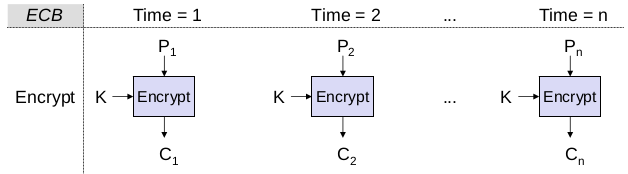
\includegraphics[width=.6\linewidth]{Assets/NetworkSecurity-electronic-code-book-mode.png}
      \end{center}

      \subsubsection{Cipher Block Chaining Mode (CBC)}
      \begin{itemize*}
            \item Vor Verschlüsselung eines Klartextblocks $P_i$ wird dieser mit dem vorangegangenen Chiffretextblock $C_{i-1}$ XOR-verknüpft
            \begin{itemize*}
                  \item $C_i = E(K, C_{i-1} \oplus P_i)$
                  \item $P_{i'} = C_{i-1} \oplus D(K, C_i)$
                  \item Um $C_1$ zu berechnen, einigen sich beide Parteien auf einen Anfangswert (IV) für $C_0$
            \end{itemize*}
            \item Fehlerfortpflanzung: Ein verfälschter Chiffretextblock führt zu zwei verfälschten Klartextblöcken, da $P_i'$ aus $C_{i-1}$ und $C_i$
            \item Synchronisation: Wenn die Anzahl der verlorenen Bits ein ganzzahliges Vielfaches von b ist, wird ein zusätzlicher Block $P_{i+1}$ verzerrt, bevor die Synchronisation wiederhergestellt wird %Wenn eine andere Anzahl von Bits verloren geht, ist eine explizite Neusynchronisation erforderlich
            \item Vorteil: identische Klartextblöcke werden zu nicht-identischem Chiffretext verschlüsselt
      \end{itemize*}
      \begin{center}
            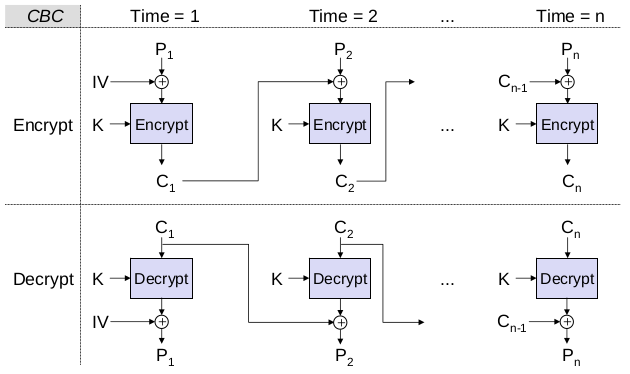
\includegraphics[width=.6\linewidth]{Assets/NetworkSecurity-cipher-block-chaining-mode.png}
      \end{center}

      \subsubsection{Ciphertext Feedback Mode (CFB)}
      \begin{itemize*}
            \item Ein Blockverschlüsselungsalgorithmus, der mit Blöcken der Größe b arbeitet, kann in einen Algorithmus umgewandelt werden, der mit Blöcken der Größe $j (j<b)$ arbeitet
            \begin{itemize*}
                  \item $S(j, x)$ bezeichnen die $j$ höherwertigen Bits von $x$
                  \item $P_i$, $C_i$ den $i$-ten Block von Klartext und Geheimtext der Länge $j$ bezeichnen
                  \item IV ist ein Anfangswert beider Parteien
                  \item $R_1 = IV$
                  \item $R_n = (R_{n-1}*2^j\ mod\ 2^b)\oplus C_{n-1}$
                  \item $C_n = S(j,E_K(R_n))\oplus P_n$
                  \item $S(j,E_K(R_n))\oplus C_n = S(j,E_K(R_n))\oplus S(j,E_K(R_n))\oplus P_n$
                  \item $S(j,E_K(R_n))\oplus C_n = P_n$
            \end{itemize*}
            \item Ein gängiger Wert für j ist 8 für die Verschlüsselung von einem Zeichen pro Schritt
            \item Fehlerfortpflanzung: Da die Chiffretextblöcke schrittweise durch das Register geschoben werden, verfälscht ein fehlerhafter Block $C_i$ den wiederhergestellten Klartextblock $P_i'$ sowie die folgenden $\lceil b / j\rceil$-Blöcke
            \item Synchronisation: Wenn die Anzahl der verlorenen Bits ein ganzzahliges Vielfaches von j ist, werden $\lceil b / j\rceil$ zusätzliche Blöcke verfälscht, bevor die Synchronisation wiederhergestellt ist% Wenn eine beliebige andere Anzahl von Bits verloren geht, ist eine explizite Neusynchronisierung erforderlich
            \item Nachteil: Die Verschlüsselungsfunktion E muss häufiger berechnet werden, da eine Verschlüsselung von $b$ Bit durchgeführt werden muss, um $j$ Bit des Klartextes zu verbergen
            %\item Beispiel: Bei Verwendung von DES mit Verschlüsselung von jeweils einem Zeichen $\Rightarrow$ muss die Verschlüsselung 8-mal häufiger durchgeführt werden
      \end{itemize*}

      \subsubsection{Output-Feedback-Modus (OFB)}
      \begin{itemize*}
            \item Pseudozufallsfolge $R_i$ verwendet, die nur von $K$ und $IV$ abhängt
            \begin{itemize*}
                  \item $S(j, x)$ bezeichnen die $j$ höherwertigen Bits von $x$
                  \item $P_i$, $C_i$ bezeichnen den $i$-ten Block von Klartext und Chiffretext der Länge $j$
                  \item $IV$ sei ein Anfangswert beider Parteien
                  \item $R_1 = IV$
                  \item $R_n = (R_{n-1}* 2^j\ mod\ 2^b )\oplus S(j,E_K(R_{n-1}))$ %// j-bit Linksverschiebung + verschlüsselter alter Wert
                  \item $C_n = S(j,E_K(R_n))\oplus P_n$
                  \item $S(j,E_K(R_n))\oplus C_n = S(j,E_K(R_n))\oplus S(j,E_K(R_n))\oplus P_n$
                  \item $S(j,E_K(R_n))\oplus C_n = P_n$
            \end{itemize*}
            \item Der Klartext wird mit der Pseudo-Zufallssequenz XOR-verknüpft, um den Chiffretext zu erhalten und umgekehrt
            \item Fehlerfortpflanzung: Einzelbitfehler führen nur zu Einzelbitfehlern $\rightarrow$ keine Fehlermultiplikation
            \item Synchronisierung: Wenn einige Bits verloren gehen, ist eine explizite Re-Synchronisation erforderlich
            \item Vorteil: Die Pseudo-Zufallsfolge kann vorberechnet werden, um die Auswirkungen der Verschlüsselung auf die Ende-zu-Ende-Verzögerung gering zu halten
            \item Verschlüsselungsfunktion muss häufiger berechnet werden, da eine Verschlüsselung von $b$ Bit durchgeführt werden muss, um $j$ Bit des Klartextes zu verbergen
            \item Es ist für einen Angreifer möglich, bestimmte Bits des Klartextes zu manipulieren
      \end{itemize*}
      \begin{center}
            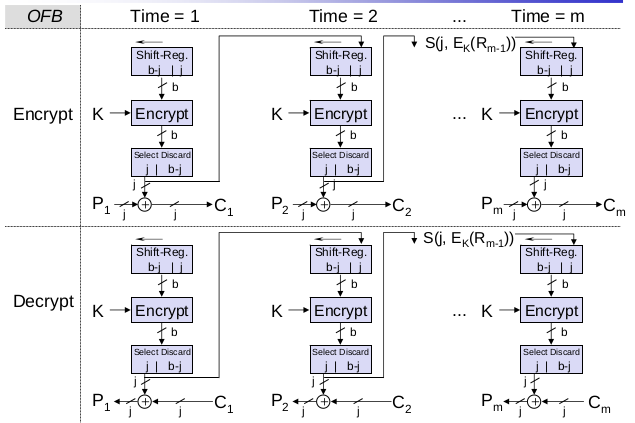
\includegraphics[width=.6\linewidth]{Assets/NetworkSecurity-output-feedback-mode.png}
      \end{center}

      \subsection{Datenverschlüsselungsstandard (DES)}
      \begin{itemize*}
            \item symmetrische Blockchiffre mit Blöcken der Länge 128 Bit
            \item unter Verwendung von Schlüsseln der Länge 128 Bit
            \item NSA reduzierte Blockgröße auf 64 Bit, die Größe des Schlüssels auf 56 Bit und änderte Details in den Substitutionsfeldern
      \end{itemize*}
      % 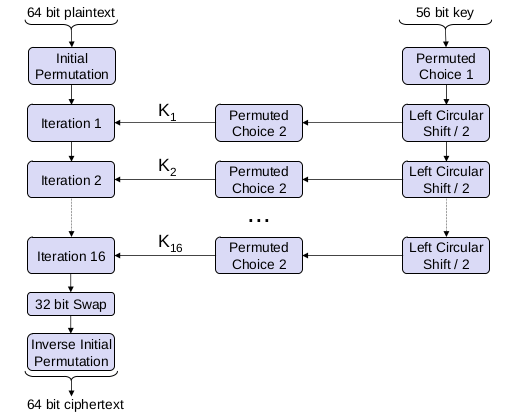
\includegraphics[width=\linewidth]{Assets/NetworkSecurity-des-algorithm.png}
      \begin{center}
            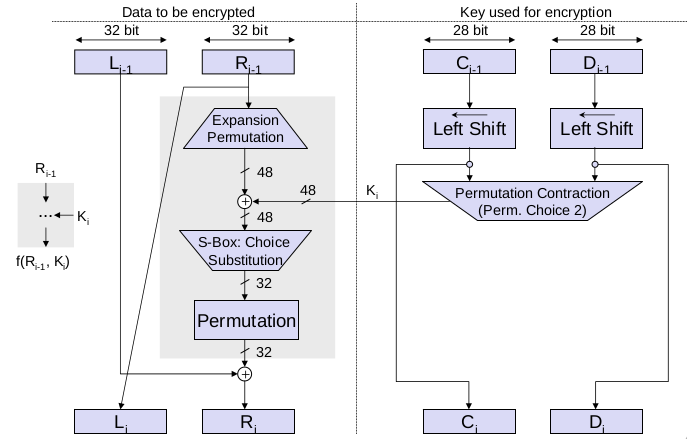
\includegraphics[width=.6\linewidth]{Assets/NetworkSecurity-des-single-iteration.png}
      \end{center}

      \subsubsection{DES - Einzelne Iteration}
      \begin{itemize*}
            \item Die rechten 32 Bit der zu verschlüsselnden Daten werden mit Hilfe einer Expansions-/Permutationstabelle auf 48 Bit erweitert
            \item linke und rechte 28 Bit des Schlüssels werden zirkulär nach links verschoben und der resultierende Wert wird mit Hilfe einer Permutations-/Kontraktionstabelle auf 48 Bit verkürzt
            \item beide oben genannten Werte XOR-verknüpft und in Auswahl- und Ersetzungsbox eingegeben
            \item Intern wird diese Operation durch 8 so genannte s-Boxen realisiert, von denen jede einen Sechs-Bit-Wert auf einen Vier-Bit-Wert gemäß einer boxspezifischen Tabelle abbildet, was insgesamt zu einem 32-Bit-Ausgang führt
            \item Ausgang des obigen Schritts wird erneut permutiert und mit den linken 32 Bit der Daten XOR-verknüpft, was zu den neuen rechten 32 Bit der Daten führt
            \item Die neuen linken 32 Bit der Daten sind der rechte Wert der vorherigen Iteration
      \end{itemize*}

      \subsubsection{DES - Entschlüsselung}
      \begin{itemize*}
            \item Unter Verwendung der Abkürzung $f(R, K)$ kann der Verschlüsselungsprozess wie folgt geschrieben werden
            \begin{itemize*}
                  \item $L_i = R_{i-1}$
                  \item $R_i = L_{i-1}\oplus f(R_{i-1}, K_i)$
                  \item Aufteilung der Daten in zwei Hälften und Organisation der Verschlüsselung gemäß den obigen Gleichungen
                  \item wird als Feistel-Netzwerk bezeichnet
            \end{itemize*}
            \item Der DES-Entschlüsselungsprozess ist im Wesentlichen derselbe wie die Verschlüsselung. Er verwendet den Chiffretext als Eingabe für den Verschlüsselungsalgorithmus, wendet aber die Unterschlüssel in umgekehrter Reihenfolge an
            \item Die Ausgangswerte sind also
            \begin{itemize*}
                  \item $L_0' || R_0' =$ InitialPermutation (Chiffretext)
                  \item Chiffretext = InverseInitialPermutation ($R_{16} || L_{16}$)
                  %\item $L_0' || R_0' =$ InitialPermutation (InverseInitialPermutation ($R_{16}|| L_{16}))=R_{16}|| L_{16}$
            \end{itemize*}
            \item Nach einem Schritt der Entschlüsselung
            \begin{itemize*}
                  \item $L_1' = R_0' = L_{16} = R_{15}$
                  \item $R_1' = L_0' \oplus f(R_0', K_{16})=R_{16}\oplus f(R_{15},K_{16})=,,L_{15}\oplus f(R_{15},K_{16})''\oplus f(R_{15},K_{16}) =L_{15}$
            \end{itemize*}
            \item Diese Beziehung gilt für den gesamten Prozess als
            \begin{itemize*}
                  \item $R_{i-1} = L_i$
                  \item $L_{i-1} = R_i\oplus f(R_{i-1}, K_i) = R_i\oplus f(L_i, K_i)$
            \end{itemize*}
            \item Der Ausgang der letzten Runde ist schließlich
            \begin{itemize*}
                  \item $L_{16}' || R_{16}' = R_0 || L_0$
            \end{itemize*}
            \item Nach der letzten Runde führt DES einen 32-Bit-Tausch und die inverse
            Anfangspermutation durch
            \begin{itemize*}
                  \item InverseInitialPermutation($L_0|| R_0$) = InverseInitialPermutation(InitialPermutation(Klartext)) = Klartext
            \end{itemize*}
      \end{itemize*}

      \subsubsection{DES - Sicherheit}
      \begin{itemize*}
            \item Schwächen der Schlüssel
            \begin{itemize*}
                  \item Schwache Schlüssel: Vier Schlüssel sind schwach, da sie Unterschlüssel erzeugen, die entweder alle 0 oder alle 1 enthalten.
                  \item Halbschwache Schlüssel: Es gibt sechs Schlüsselpaare, die Klartext zu identischem Chiffriertext verschlüsseln, da sie nur zwei verschiedene Unterschlüssel erzeugen
                  \item Möglicherweise schwache Schlüssel: Es gibt 48 Schlüssel, die nur vier verschiedene Unterschlüssel erzeugen
                  \item Insgesamt werden $64$ von $72057594037927936$ als schwach angesehen
            \end{itemize*}
            \item Algebraische Struktur
            \begin{itemize*}
                  \item Wäre DES geschlossen, dann gäbe es für jedes $K_1,K_2$ ein $K_3$, so dass: $E(K_2,E(K_1,M))=E(K_3,M)$, also wäre die doppelte Verschlüsselung nutzlos
                  \item Wäre DES rein, dann gäbe es für jedes $K_1,K_2,K_3$ ein $K_4$, so dass $E(K_3,E(K_2,E(K_1,M)))=E(K_4,M)$, also wäre die dreifache Verschlüsselung nutzlos
                  \item DES ist weder geschlossen noch rein, daher kann ein Mehrfachverschlüsselungsschema verwendet werden, um die Schlüssellänge zu erhöhen
            \end{itemize*}
            \item Differentielle Kryptoanalyse
            \begin{itemize*}
                  \item Im Jahr 1990 veröffentlichten E. Biham und A. Shamir diese Analysemethode
                  \item Sie sucht gezielt nach Unterschieden in Chiffretexten, deren Klartexte bestimmte Unterschiede aufweisen, und versucht, daraus den richtigen Schlüssel zu erraten
                  \item Der grundlegende Ansatz benötigt einen ausgewählten Klartext zusammen mit seinem Chiffretext
                  \item DES mit 16 Runden ist gegen diesen Angriff immun, da der Angriff $2^{47}$ gewählte Klartexte oder $2^{55}$ bekannte Klartexte benötigt
                  \item Die Entwickler von DES erklärten in den 1990er Jahren, dass sie in den 1970er Jahren über diese Art von Angriffen Bescheid wussten und dass die s-Boxen entsprechend entworfen wurden
            \end{itemize*}
            \item Schlüssellänge:  Da 56-Bit-Schlüssel in $10,01$ Stunden durchsucht werden kann, wenn man $10^6$ Verschlüsselungen/$\mu s$ durchführen kann, kann DES nicht mehr als ausreichend sicher angesehen werden
      \end{itemize*}

      \subsubsection{Erweiterung der Schlüssellänge von DES}
      \begin{itemize*}
            \item Doppelter DES: Da DES nicht geschlossen ist, führt die doppelte Verschlüsselung zu einer Chiffre, die 112-Bit-Schlüssel verwendet
            \begin{itemize*}
                  \item kann mit Aufwand von $2^{56}$ angegriffen werden.
                  \item Da $C=E(K_2,E(K_1,P)) \Rightarrow X:=E(K_1,P)=D(K_2,C)$
                  \item Wenn ein Angreifer ein bekanntes Klartext/Chiffretext-Paar erhalten kann, kann er zwei Tabellen erstellen (meet-in-the-middle-attack)
                  \begin{itemize*}
                        \item Tabelle 1 enthält die Werte von $X$, wenn $P$ mit allen möglichen Werten von $K$ verschlüsselt ist
                        \item Tabelle 2 enthält die Werte von $X$, wenn $C$ mit allen möglichen Werten von $K$ entschlüsselt wird
                        \item Sortiere die beiden Tabellen und konstruiere Schlüssel $K_{T1}|| K_{T2}$ für alle Kombinationen von Einträgen, die den gleichen Wert ergeben.
                  \end{itemize*}
            \end{itemize*}
            \item Da es für jeden beliebigen Klartext $2^{64}$ mögliche Chiffretext-Werte gibt, die mit Double-DES erzeugt werden könnten, gibt es beim ersten bekannten Klartext/Chiffretext-Paar durchschnittlich $2^{112}/2^{64}=2^{48}$ Fehlalarme
            \item Jedes weitere Klartext/Chiffretext-Paar verringert die Chance, einen falschen Schlüssel zu erhalten, um den Faktor $1/2^{64}$, so dass bei zwei bekannten Blöcken die Chance $2^{-16}$ beträgt
            \item Der Aufwand, der erforderlich ist, um Double DES zu knacken, liegt also in der Größenordnung von $2^{56}$, was nur geringfügig besser ist als der Aufwand von $2^{55}$, der erforderlich ist, um Single DES mit einem Angriff mit bekanntem Klartext zu knacken, und weit entfernt von den $2^{111}$, die wir von einer Chiffre mit einer Schlüssellänge von 112 Bit erwarten würden
            \item Diese Art von Angriff kann durch die Verwendung eines dreifachen Verschlüsselungsschemas umgangen werden, wie es 1979 von W. Tuchman vorgeschlagen wurde
            \item $C=E(K_3,D(K_2,E(K_1,P)))$
            \item Die Verwendung der Entschlüsselungsfunktion D in der Mitte ermöglicht die Verwendung von Dreifachverschlüsselungsgeräten mit Gegenstellen, die nur Einfachverschlüsselungsgeräte besitzen, indem $K_1=K_2=K_3$ gesetzt wird
            \item Dreifachverschlüsselung kann mit zwei (Einstellung $K_1=K_3$) oder drei verschiedenen Schlüsseln verwendet werden
            \item Bislang keine praktischen Angriffe gegen dieses Verfahren bekannt
            \item Nachteil: die Leistung beträgt nur $1/3$ der einfachen Verschlüsselung, so dass es besser sein könnte, gleich eine andere Chiffre zu verwenden, die eine größere Schlüssellänge bietet
      \end{itemize*}

      \subsection{Fortgeschrittener Verschlüsselungsstandard AES}
      \begin{itemize*}
            \item Oktober 2000: Rijndael als Vorschlag des NIST für AES
            \item Rundenbasierte symmetrische Chiffre
            \item Keine Feistel-Struktur (versch. Ver- und Entschlüsselung)
            \item Schlüssellänge: 128, 192, oder 256 Bit
            \item Blocklänge: 128, 192 oder 256 Bit (nur 128 standardisiert)
            \item Anzahl der Runden: 10, 12, 14
            \item Der Algorithmus arbeitet mit
            \begin{itemize*}
                  \item $state[4, 4]$: ein Byte-Array mit 4 Zeilen und 4 Spalten %(für 128-Bit-Blockgröße)
                  \item $key[4, 4]$: ein Array mit 4 Zeilen und 4 Spalten %(für 128-Bit-Schlüsselgröße)
            \end{itemize*}
            \item Verschlüsselung: (für eine Block- und Schlüsselgröße von 128 Bit) in Runden $1-9$ werden vier Operationen verwendet
            \begin{description*}
                  \item[ByteSub] nicht-lineare Byte-Substitution durch feste Tabelle (s-Box)
                  \item[ShiftRow] Zeilen des Zustands zyklisch um verschiedene Offsets verschoben
                  \item[MixColumn] die Spalten von $state[]$ werden als Polynome über $GF(2^8)$ betrachtet und modulo $x^4+1$ mit einer festen Matrix multipliziert: $\begin{pmatrix} 02&03&01&01\\ 01&02&03&01 \\ 01&01&02&03\\ 03&01&01&02 \end{pmatrix}$
                  \item[RoundKey] ein Round-Key wird mit dem Status XORiert
                  \item[Runde 10] nutzt Operation MixColumn NICHT
            \end{description*}
            % 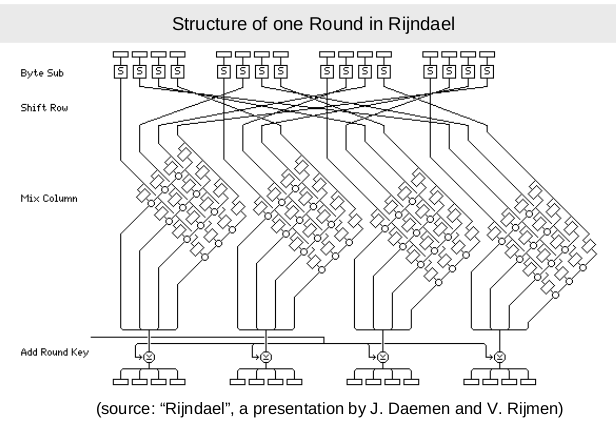
\includegraphics[width=\linewidth]{Assets/NetworkSecurity-rijndael-one-round.png}
            \item Entschlüsselung
            \begin{itemize*}
                  \item Rundenschlüssel und Operationen in umgekehrter Reihenfolge
                  \item MixColumn-Schritt kann nur durch Multiplikation mit der inversen Matrix (auch über $GF(2^8)$) invertiert werden
                  \item $\begin{pmatrix} 0e&0b&0d&09\\ 09&0e&0b&0d\\ 0d&09&0e&0b\\ 0b&0d&09&0e \end{pmatrix}$
                  \item Oft werden tabellarische vorberechnete Lösungen verwendet, die mehr Platz benötigen
            \end{itemize*}
      \end{itemize*}

      Sicherheit
      \begin{itemize*}
            %\item Die einfache mathematische Struktur von AES ist der Hauptgrund für seine Geschwindigkeit, führte aber auch zu Kritik
            \item Nur die ByteSub-Funktion ist wirklich nichtlinear und verhindert effektive Analyse
            \item AES kann als große Matrix-Operation beschrieben werden
            \item Bereits während der Standardisierung wurden Angriffe für reduzierte Versionen entwickelt
            \begin{itemize*}
                  \item Ein Angriff mit $2^{32}$ gewähltem Klartext gegen eine 7-Runden-Version von AES
                  \item Signifikante Reduktion der Komplexität auch für eine 9-Runden-Version von AES mit 256-Schlüsselgröße mit einem zugehörigen Schlüsselangriff
            \end{itemize*}
            \item 2011 erster Angriff gegen vollständigen AES bekannt
            \begin{itemize*}
                  \item Schlüsselwiederherstellung in $2^{126.1}$ für AES mit 128 Bit, $2^{189.7}$ für AES mit 192 Bit, $2^{254.4}$ für AES mit 256 Bit
                  \item Praktischer Angriff (geht nicht von verwandten Schlüsseln aus)
                  \item nur ein kleiner Kratzer in Anbetracht von 10 Jahren kryptographischer Forschung
            \end{itemize*}
      \end{itemize*}

      \subsection{Stromchiffre-Algorithmus RC4}
      \begin{itemize*}
            \item Stromchiffre, die 1987 von Ron Rivest erfunden wurde
            \item RC4 wird im Output-Feedback-Modus (OFB) betrieben
            \begin{itemize*}
                  \item Der Verschlüsselungsalgorithmus erzeugt eine Pseudozufallsfolge $RC4(IV,K)$, die nur vom Schlüssel K und einem Initialisierungsvektor IV abhängt
                  \item Der Klartext $P_i$ wird dann mit der Pseudozufallssequenz XOR-verknüpft, um den Chiffretext zu erhalten %und umgekehrt
                  \item $C_1 = P_1\oplus RC4 (IV_1,K)$
                  \item $P_1 = C_1\oplus RC4 (IV_1,K)$
            \end{itemize*}
            \item Pseudo-Zufallsfolge wird oft als Keystream bezeichnet
            \item Keystream niemals wiederverwenden, entscheidend für Sicherheit (XOR zweier Klartexte erhalten)
            %\item Wenn der Keystream wiederverwendet wird (d.h. $IV_1=IV_2$ mit demselben $K$), dann kann das XOR zweier Klartexte erhalten werden %$C_1\oplus C_2= P_1\oplus RC4(IV, K)\oplus P_2\oplus RC4(IV,K) = P_1\oplus P_2$
            \item RC4 verwendet einen Schlüssel variabler Länge bis zu 2048 Bit
            \item Eig. dient Schlüssel als Seed für Pseudo-Zufallsgenerator
            \item RC4 arbeitet mit zwei 256-Byte-Arrays: $S[0,255], K[0,255]$
            \begin{enumerate*}
                  \item Initialisierung der Arrays
                  %\begin{Shaded} % \begin{Highlighting}[] % \ControlFlowTok{for}\NormalTok{ (i = }\DecValTok{0}\NormalTok{; i < }\DecValTok{256}\NormalTok{; i++){} % \NormalTok{ S[i] = i; }\CommentTok{// Array S[] mit 0 bis 255 füllen} % \NormalTok{}} % \CommentTok{// Füllen des Arrays K[] mit dem Schlüssel und IV durch Wiederholung, bis K[] gefüllt ist} % \NormalTok{n = }\DecValTok{0}\NormalTok{;} % \ControlFlowTok{for}\NormalTok{ (i =}\DecValTok{0}\NormalTok{; i < }\DecValTok{256}\NormalTok{; i++) {} % \NormalTok{ n = (n + S[i] + K[i]) MOD }\DecValTok{256}\NormalTok{; swap(S[i], S[n]); } % \NormalTok{}} % \end{Highlighting} %\end{Shaded}
                  \item Erzeugen des Schlüsselstroms (nach Init $i=0;n=0;$)
                  %\begin{Shaded} % \begin{Highlighting}[] % \NormalTok{i = (i + }\DecValTok{1}\NormalTok{) MOD }\DecValTok{256}\NormalTok{; n = (n + S[i]) MOD }\DecValTok{256}\NormalTok{;} % \NormalTok{swap(S[i], S[n]);} % \NormalTok{t = (S[i] + S[n]) MOD }\DecValTok{256}\NormalTok{;} % \NormalTok{Z = S[t]; }\CommentTok{// Z enthält 8 Bit des durch eine Iteration erzeugten Schlüsselstroms} % \end{Highlighting} %\end{Shaded}
                  \item XOR-Verknüpfung des Schlüsselstroms mit dem Klartext% oder Chiffretext
            \end{enumerate*}
            \item Sicherheit von RC4
            \begin{itemize*}
                  \item Sicherheit gegen Brute-Force-Angriffe
                  \item variable Schlüssellänge bis 2048 Bit
                  \item durch Verringerung der Schlüssellänge beliebig unsicher
                  \item RSA Data Security Inc. behauptet, RC4 sei immun gegen differentielle und lineare Kryptoanalyse und es seien keine kleinen Zyklen bekannt
            \end{itemize*}
            \item RC4 mit 40-Bit-Schlüsseln hatte einen besonderen Exportstatus%, selbst als andere Chiffren nicht aus den USA exportiert werden durften
            \begin{itemize*}
                  \item SSL verwendet RC4 mit 40-Bit-Schlüsseln %als Standardalgorithmus
                  \item Schlüssellänge von 40 Bit nicht immun gegen Brute-Force
            \end{itemize*}
            \item Je nach Schlüsselplanung kann RC4 stark verwundbar sein
            \item empfohlen min. erste 3072 Bytes des Schlüsselstroms zu verwerfen
            \item sollte nicht mehr verwendet werden%, auch nicht bei längeren Schlüsseln
      \end{itemize*}

      \subsection{KASUMI}
      \begin{itemize*}
            \item Verwendet zur Verschlüsselung von Anrufen in GSM und UMTS
            \item Entwickelt für Hardware-Implementierung ($<10k$ Gatter)
            \item Schnelle Implementierung möglich
            \item 64-Bit-Blockgröße, 128-Bit-Schlüssellänge
            \item 8 Runden Feistel-Netzwerk
            \item Sicherheitsspanne nicht sehr groß
      \end{itemize*}
      \begin{center}
            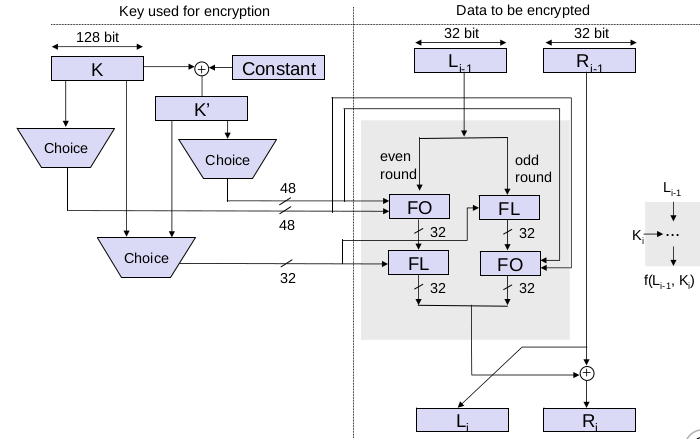
\includegraphics[width=.6\linewidth]{Assets/NetworkSecurity-kasumi-singe-iteration.png}
      \end{center}
      \begin{itemize*}
            \item linke 32 Bit der zu verschlüsselnden Daten werden durch zwei nichtlineare Funktionen FO und FL verändert, die beide Schlüsselmaterial verwenden
            \item Reihenfolge, in der FO und FL angewendet werden, hängt von Rundenzahl ab
            \item FL teilt die Daten in 16-Bit-Wörter auf, die mit Schlüsselmaterial kombiniert, permutiert und mit den Originalwerten XOR-verknüpft werden
            \item FO ist ein 3-Runden-Feistel-Netzwerk mit einer Modifizierungsfunktion FI, die selbst ein Feistel-ähnliches Netzwerk ist, das zwei s-Boxen verwendet
            \item Der Ausgang des obigen Schritts wird mit den rechten 32 Bit der Daten XOR-verknüpft, was zu den neuen rechten 32 Bit der Daten führt
            \item neue linke 32-Bit der Daten ist rechte Wert der vorherigen Iteration
      \end{itemize*}

      Sicherheit
      \begin{itemize*}
            \item reduzierte Version (6 Runden) kann durch unmögliche differentielle Kryptoanalyse angegriffen werden, bei der unmögliche Zustände der Chiffre aus Chiffretext/Klartext-Paaren abgeleitet werden (Zeitkomplexität von $2^{100}$)
            %\begin{itemize*}
            %\item Erste Veröffentlichung bereits ein Jahr nach der Standardisierung
            %\end{itemize*}
            \item Für Vollversion von KASUMI verwandte Schlüsselangriffe möglich
            \begin{itemize*}
                  \item Ausgewählter Klartextangriff, bei dem der Angreifer dieselben Daten mit mehreren ,,verwandten'' Schlüsseln verschlüsseln kann
                  \item Zeitkomplexität von $2^{76.1}$ und $2^{32}$ im besten Fall
                  \item Bedingungen, unter denen Angreifer Zugang zu verwandten Schlüsseln in 3G-Netzen haben, sehr selten
                  %\item MISTY von diesen Angriffen nicht betroffen
            \end{itemize*}
            \item ETSI hat jedoch SNOW 3G eingeführt, um auf eine vollständige Verletzung von KASUMI vorbereitet zu sein
            \begin{itemize*}
                  \item Stromchiffre basierend auf LFSR, in 7.500 ASIC-Gattern %implementiert
                  \item anfällig für verwandte Schlüsselangriffe
            \end{itemize*}
      \end{itemize*}

      \section{Asymmetrische Kryptographie}
      \begin{itemize*}
            \item zwei verschiedene Schlüssel $-K$ und $+K$
            \item mit Chiffretext $c=E(+K, m)$ und $+K$ sollte es nicht möglich sein, $m=D(-K,c) =D(-K,E(+K,m))$ zu berechnen
            \item Berechnung von $-K$ bei $+K$ nicht möglich sein sollte
            \item $-K_A$ nur einer Entität A bekannt, privater Schlüssel
            \item $+K_A$ öffentlich bekannt, öffentlicher Schlüssel
            \begin{description*}
                  \item[Verschlüsselung] Nachricht mit $+K_A$ verschlüsselt, kann nur mit $-K_A$ entschlüsselT werden
                  \item[Signieren] Nachricht mit $-K_A$ verschlüsselt, kann jeder Signatur mit $+K_A$ verifizieren
                  \item[Achtung] Entscheidend ist, dass jeder nachprüfen kann, dass er wirklich den öffentlichen Schlüssel von A kennt und nicht den Schlüssel eines Gegners
            \end{description*}
            \item Entwurf von asymmetrischen Kryptosystemen
            \begin{itemize*}
                  \item Finde einen Algorithmus und eine Methode, zwei Schlüssel $-K$, $+K$ so zu konstruieren, dass es nicht möglich ist, $E(+K, m)$ mit der Kenntnis von $+K$ zu entschlüsseln
                  \item Schlüssellänge sollte ,,überschaubar'' sein
                  \item Verschlüsselte Nachrichten sollten nicht beliebig länger sein als unverschlüsselte Nachrichten
                  \item Ver- und Entschlüsselung sollten nicht zu viele Ressourcen verbrauchen (Zeit, Speicher)
                  \item Idee: Man nehme ein Problem aus dem Bereich der Mathematik/Informatik, das schwer zu lösen ist, wenn man nur $+K$ kennt, aber leicht zu lösen, wenn man $-K$ kennt
            \end{itemize*}
      \end{itemize*}
      \begin{description*}
            \item[Knapsack-Probleme] Grundlage der ersten funktionierenden Algorithmen, leider fast alle als unsicher erwiesen
            \item[Faktorisierungsproblem] Grundlage des RSA-Algorithmus
            \item[Diskreter-Logarithmus-Problem] Grundlage von Diffie-Hellman und ElGamal
      \end{description*}

      \subsection{Einige mathematische Hintergründe}
      \begin{itemize*}
            \item Sei $\mathbb{Z}$ die Menge der ganzen Zahlen, und $a,b,n\in\mathbb{Z}$
            \item $a$ teilt $b(a| b)$ wenn es eine ganze Zahl $k\in\mathbb{Z}$ gibt, so dass $a\times k=b$
            \item $a$ ist prim, wenn a positiv und einzige Teiler von a $1$ und $a$
            \item $r$ ist der Rest von a geteilt durch $n$, wenn $r=a-\lfloor a / n \rfloor\times n$, wobei $\lfloor x\rfloor$ die größte ganze Zahl kleiner oder gleich $x$ ist
            %\begin{itemize*}
            %      \item Beispiel: 4 ist der Rest von 11 geteilt durch 7 als $4=11-\lfloor 11/7\rfloor\times 7$
            %      \item Wir können dies auch anders schreiben: $a=q\times n + r$ mit $q=\lfloor a/n\rfloor$
            %\end{itemize*}
            \item Für Rest $r$ von a durch n schreiben wir $a\ MOD\ n$
            \item b ist kongruent $a\ mod\ n$, wenn es bei der Division durch n den gleichen Rest wie a hat. Also teilt n $(a-b)$, und wir schreiben $b\equiv a\ mod\ n$
            %\item Beispiele: $4\equiv 11\ mod\ 7$, $25\equiv 11\ mod\ 7$, $11\equiv 25\ mod\ 7$, $11\equiv 4\ mod\ 7$, $-10\equiv 4\ mod\ 7$
            \item Da der Rest r der Division durch n immer kleiner als n ist, stellt man manchmal die Menge ${x\ mod\ n | x\in\mathbb{Z}}$ durch Elemente der Menge $\mathbb{Z}_n={0, 1, ..., n-1}$ dar
      \end{itemize*}

      \begin{tabular}{l|l}
            Eigenschaft & Ausdruck                                                                                                          \\\hline
            Kommutativ  & $(a + b)\ mod\ n = (b+ a)\ mod\ n$                                                                                \\
                        & $(a \times b)\ mod\ n = (b \times a)\ mod\ n$                                                                     \\
            Assoziativ  & $[(a + b) + c]\ mod\ n =[a + (b + c)]\ mod\ n$                                                                    \\
                        & $[(a \times b) \times c]\ mod\ n =[a \times (b \times c)]\ mod\ n$                                                \\
            Distributiv & $[a \times (b + c)]\ mod\ n =[(a \times b) + (a \times c)]\ mod\ n$                                               \\
            Identitäten & $(0 + a)\ mod\ n = a\ mod\ n$                                                                                     \\
                        & $(1 \times a)\ mod\ n = a\ mod\ n$                                                                                \\
            Inverse     & $\forall a \in \mathbb{Z}n: \exists (-a)\in \mathbb{Z}n : a + (-a) \equiv 0\ mod\ n$                              \\
                        & p is prime $\Rightarrow \forall a\in \mathbb{Z}p: \exists (a-1) \in \mathbb{Z}p: a \times (a-1) \equiv 1\ mod\ p$
      \end{tabular}

      Größter gemeinsamer Teiler
      \begin{itemize*}
            %\item $c = gcd(a, b) :\Leftrightarrow ( c | a) \wedge ( c | b) \wedge ,,\forall d: ( d | a ) \wedge ( d | b) \Rightarrow ( d | c )''$ und $gcd(a, 0 ) : = | a |$
            \item Der gcd-Rekursionssatz $\forall a, b \in \mathbb{Z}^+: gcd(a, b) = gcd(b, a\ mod\ b)$
            %\item Da $gcd(a, b)$ sowohl a als auch b teilt, teilt es auch jede Linearkombination von ihnen%, insbesondere $(a- \lfloor a / b \rfloor \times b) = a\ mod\ b$, also $gcd(a, b) | gcd(b, a\ mod\ b)$
            %\item Da $gcd(b, a\ mod\ b)$ sowohl b als auch $a\ mod\ b$ teilt, teilt es auch jede Linearkombination von beiden, insbesondere $\lfloor a / b \rfloor \times b + (a\ mod\ b) = a$, also $gcd(b, a\ mod\ b) | gcd(a, b)$
            %\item Euklidischer Algorithmus: aus $a, b$ berechnet $gcd(a, b)$
            %\begin{Shaded}
            % \begin{Highlighting}[]
            % \DataTypeTok{int}\NormalTok{ Euclid(}\DataTypeTok{int}\NormalTok{ a, b){}
            % \ControlFlowTok{if}\NormalTok{ (b = }\DecValTok{0}\NormalTok{) { }\ControlFlowTok{return}\NormalTok{(a); }}
            % \NormalTok{ {}\ControlFlowTok{return}\NormalTok{(Euclid(b, a\ mod\ b);} }
            % \NormalTok{}}
            % \end{Highlighting}
            %\end{Shaded}
            \item Erweiterter euklidischer Algorithmus%: für $a, b$ berechnet  $d, m, n$ so, dass $d = gcd(a, b) = m \times a + n \times b$
            %\begin{Shaded}
            % \begin{Highlighting}[]
            % \KeywordTok{struct}\NormalTok{{}\DataTypeTok{int}\NormalTok{ d, m, n} ExtendedEuclid(}\DataTypeTok{int}\NormalTok{ a, b)}
            %% \NormalTok{{ }\DataTypeTok{int}\NormalTok{ d, d}\CharTok{\textquotesingle{},}\ErrorTok{ m, m}\CharTok{\textquotesingle{}}\NormalTok{, n, n}\CharTok{\textquotesingle{};}
            % \ControlFlowTok{if}\NormalTok{ (b = }\DecValTok{0}\NormalTok{) {}\ControlFlowTok{return}\NormalTok{(a, }\DecValTok{1}\NormalTok{, }\DecValTok{0}\NormalTok{); }}
            % \NormalTok{ (d}\CharTok{\textquotesingle{},}\ErrorTok{ m}\CharTok{\textquotesingle{}}\NormalTok{, n}\CharTok{\textquotesingle{})}\ErrorTok{ = ExtendedEuclid(b, a MOD b);}
            % \NormalTok{ (d, m, n) = (d}\CharTok{\textquotesingle{},}\ErrorTok{ n}\CharTok{\textquotesingle{}}\NormalTok{, m}\CharTok{\textquotesingle{} }\ErrorTok{{-} \\lfloor a / b \\rfloor \\times n}\CharTok{\textquotesingle{}}\NormalTok{);}
            % \ControlFlowTok{return}\NormalTok{(d, m, n); }}
            % \end{Highlighting}
            %\end{Shaded}
            \begin{itemize*}
                  \item Grundfall $(a,0): gcd(a, 0) = a = 1 \times a + 0 \times 0$
                  \item Induktion von $(b, a\ mod\ b)$ auf $(a, b)$
                  \begin{itemize*}
                        \item ExtendedEuclid berechnet $d', m', n'$ korrekt
                        \item $d=d'=m'\times b+n'\times (a\ mod\ b)=m'\times b+n'\times (a-\lfloor a/b\rfloor\times b)=n'\times a+(m'-\lfloor a/b\rfloor\times n')\times b$
                  \end{itemize*}
                  \item Laufzeit von $Euclid$ und $ExtendedEuclid$ ist $O(log\ b)$
            \end{itemize*}
            \item Lemma: Sei $a,b\in\mathbb{N}$ und $d=gcd(a,b)$. Dann gibt es $m,n\in\mathbb{N}$ so, dass: $d=m\times a+n \times b$
            \item Euklid: Wenn eine Primzahl das Produkt zweier ganzer Zahlen teilt, dann teilt sie mindestens eine der ganzen Zahlen: $p|(a\times b)\Rightarrow (p| a)\times(p| b)$
            %\begin{itemize*}
            %      \item Der Beweis: Es sei $p|(a\times b)$
            %      \item Wenn $p| a$ dann sind wir fertig
            %      \item Wenn nicht, dann $gcd(p,a) = 1 \Rightarrow\exists m, n\in\mathbb{N}:1=m\times p+n\times a \Leftrightarrow b=m\times p \times b + n \times a \times b$
            %      \item Da $p|(a\times b)$, teilt p beide Summanden der Gleichung und somit auch die Summe, die b ist
            %\end{itemize*}
            \item Fundamentalsatz der Arithmetik: Die Faktorisierung in Primzahlen ist bis zur Ordnung eindeutig
            %\item verwende Theorem 2, um folgende Korollarie zu beweisen
            %\begin{itemize*}
            %      \item Wenn $gcd(c,m)=1$ und $(a\times c)\equiv(b\times c)mod\ m$, dann $a\equiv b\ mod\ m$
            %\item Der Beweis: Da $(a\times c)\equiv(b\times c)mod\ m\Rightarrow\exists n\in\mathbb{N}:(a\times c)-(b\times c)=n\times m$
            %\item $\Leftrightarrow ( a - b ) \times c = n \times m$
            %\item $\Leftrightarrow p_1\times ...\times p_i\times q_1\times ...\times q_j=r_1\times ...\times r_k\times s_1\times ...\times s_l$
            %      \item $p$, $q$, $r$ und $s$ sind Primzahlen und müssen nicht verschieden sein aber da $gcd(c,m)=1$, gibt es keine Indizes g, h, so dass $q_g = s_h$
            %\item Wir können also die Gleichung fortlaufend durch alle q's teilen, ohne jemals ein $s$ zu ,,eliminieren'' und erhalten schließlich etwas wie $\Leftrightarrow p_1\times ...\times p_i=r_1\times ...\times r_o\times s_1\times ...\times s_l$ (beachten Sie, dass es weniger r's geben wird)
            %      \item[$\Leftrightarrow$] $(a-b)=r_1\times ...\times r_o\times m\Rightarrow a \equiv b\ mod\ m$
            %\end{itemize*}
            \item Bezeichne $\phi(n)$ die Anzahl der positiven ganzen Zahlen, die kleiner als n und relativ zu n prim sind
            \begin{itemize*}
                  \item Beispiele: $\phi(4) = 2$, $\phi(6)=2$, $\phi(7)=6$, $\phi(15)=8$
                  \item Wenn p eine Primzahl ist $\Rightarrow\phi(p)=p-1$
            \end{itemize*}
            \item Euler: Seien n und b positive und relativ primäre ganze Zahlen, d.h. $gcd(n, b) = 1 \Rightarrow b \phi(n) \equiv 1\ mod\ n$
            \begin{itemize*}
                  %\item Sei $t=\phi(n)$ und $a_1,...a_t$ seien die positiven ganzen Zahlen kleiner als $n$, die relativ zu $n$ prim sind. Definieren Sie $r_1,...,r_t$ als die Residuen von $b\times a_1\ mod\ n , ..., b\times a_t\ mod\ n$, d.h.: $b\times a_i \equiv r_i\ mod\ n$.
                  \item Beachten Sie, dass $i\not= j \Rightarrow r_i\not= r_j$%. Wäre dies nicht der Fall, hätten wir $b\times a_i\equiv b\times a_j\ mod\ n$ und da $gcd(b,n)=1$, würde Korollar 1 $a_i\equiv a_j\ mod\ n$ implizieren, was nicht sein kann, da $a_i$ und $a_j$ per Definition verschiedene ganze Zahlen zwischen 0 und n sind
                  %\item Wir wissen auch, dass jedes $r_i$ relativ prim zu n ist, denn jeder gemeinsame Teiler k von $r_i$ und $n$ , d.h. $n=k\times m$ und $r_i=p_i\times k$, müsste auch $a_i$ teilen,
                  %\item da $b\times a_i$gleich $(p_i\times k)\ mod\ (k\times m)\Rightarrow\exists s\in\mathbb{N}:(b\times a_i)-(p_i\times k)=s\times k\times m \Leftrightarrow (b\times a_i)=s\times k\times m+(p_i\times k)$
                  %\item Da k jeden der Summanden auf der rechten Seite dividiert und k nicht durch b dividiert (n und b sind relativ prim), müsste es auch $a_i$ dividieren, das relativ prim zu n sein soll
                  %\item Somit ist $r_1, ...,r_t$ eine Menge von $\phi(n)$ verschiedenen ganzen Zahlen, die relativ prim zu $n$ sind. Das bedeutet, dass sie genau dasselbe sind wie $a_1,...a_t$, nur dass sie in einer anderen Reihenfolge stehen. Insbesondere wissen wir, dass $r_1\times ...\times r_t=a_1\times ...\times a_t$
                  \item Wir verwenden nun die Kongruenz $r_1\times ...\times r_t\equiv b\times a_1\times ...\times b\times a_t\ mod\ n$ $\Leftrightarrow r_1\times ...\times r_t\equiv b_t\times a_1\times ...\times a_t\ mod\ n$ $\Leftrightarrow r_1\times ...\times r_t\equiv b_\times r_1\times ...\times r_t\ mod\ n$
                  \item Da alle $r_i$ relativ prim zu $n$ sind, können wir Korollar 1 anwenden und durch ihr Produkt dividieren: $1\equiv b_t\ mod\ n \Leftrightarrow 1\equiv b\phi(n)\ mod n$
            \end{itemize*}
            \item Chinesischer Restssatz Theorem
            \begin{itemize*}
                  \item Seien $m_1,...,m_r$ positive ganze Zahlen, die paarweise relativ prim sind,
                  \item d.h. ganz $i\not= j:gcd(m_i, m_j) = 1$. Seien $a_1,...,a_r$ beliebige ganze Zahlen
                  \item Dann gibt es eine ganze Zahl a derart, dass
                  \begin{itemize*}
                        \item $a\equiv a_1\ mod\ m_1$
                        \item $a\equiv a_2\ mod\ m_2$
                        \item ...
                        \item $a\equiv a_r\ mod\ m_r$
                  \end{itemize*}
                  \item Außerdem ist a eindeutig modulo $M := m_1\times ...\times m_r$
                  \item Für alle $i\in{1,...,r}$ definieren wir $M_i:=(M/m_i)\phi(m_i)$
                  \item Da $M_i$ per Definition relativ prim zu $m_i$ ist, können wir Theorem 3 anwenden und wissen, dass $M_i\equiv 1\ mod\ m_i$
                  \item Da $M_i$ durch $m_j$ für jedes $j\not= i$ teilbar ist, haben wir $\forall j\not= i:M_i\equiv 0\ mod\ m_j$ \item Wir können nun die Lösung konstruieren, indem wir definieren: $a:= a_1\times M_1+a_2\times M_2+...+a_r\times M_r$
                  %\item Die beiden oben angeführten Argumente bezüglich der Kongruenzen der $M_i$ implizieren, dass a tatsächlich alle Kongruenzen erfüllt
                  %\item Um zu sehen, dass a eindeutig modulo $M$ ist, sei b eine beliebige andere ganze Zahl, die die r Kongruenzen erfüllt. Da $a\equiv c\ mod\ n$ und $b\equiv c\ mod\ n \Rightarrow a \equiv b\ mod\ n$ haben wir $\forall i\in{1,...,r}:a\equiv b\ mod\ m_i\Rightarrow\forall i\in{1,. ...,r}:m_i|(a-b) \Rightarrow M|(a-b)$, da die $m_i$ paarweise relativ prim sind $\Leftrightarrow a\equiv b\ mod\ M$
            \end{itemize*}
            \item Lemma: Wenn $gcd(m,n)=1$, dann ist $\phi(m\times n)=\phi(m)\times \phi(n)$
            %\begin{itemize*}
            %\item Sei a eine positive ganze Zahl, die kleiner als und relativ prim zu $m\times n$ ist. Mit anderen Worten: a ist eine der ganzen Zahlen, die von $\phi(m\times n)$ gezählt werden.
            %\item Betracht $a\rightarrow(a\ mod\ m, a\ mod\ n)$. Die ganze Zahl $a$ ist relativ prim zu m und relativ prim zu n. Also ist $(a\ mod\ m)$ relativ prim zu m und $(a\ mod\ n)$ ist relativ prim zu n, da: $a=\lfloor a/m\rfloor\times m + (a\ mod\ m)$, wenn es also einen gemeinsamen Teiler von $m$ und $(a\ mod\ m)$ gäbe, würde dieser Teiler auch a teilen. %Somit entspricht jede Zahl a, die durch $\phi(m\times n )$ gezählt wird, einem Paar von zwei ganzen Zahlen $(a\ mod\ m,a\ mod\ n)$, wobei die erste durch $\phi(m)$ und die zweite durch $\phi(n)$ gezählt wird.
            %\item Aufgrund des zweiten Teils von Satz 4 ist die Einzigartigkeit der Lösung $a\ mod\ (m\times n)$ der simultanen Kongruenzen: $a \equiv(a\ mod\ m)\ mod\ m$, $a \equiv(a\ mod\ n)\ mod\ n$ können wir ableiten, dass verschiedene ganze Zahlen, die durch $\phi(m\times n)$ gezählt werden, verschiedenen Paaren entsprechen
            %\item Um dies zu sehen, nehmen wir an, dass $a\not=b$, gezählt durch $\phi(m\times n)$, demselben Paar $(a\ mod\ m, a\ mod\ n)$ entspricht. Dies führt zu einem Widerspruch, da b auch die Kongruenzen erfüllen würde: $b\equiv (a\ mod\ m)\ mod\ m$ $b\equiv (a\ mod\ n)\ mod\ n$ aber die Lösung dieser Kongruenzen ist eindeutig modulo $(m \times n)$
            %\item $\phi(m \times n)$ ist höchstens die Anzahl solcher Paare: $\phi(m \times n)\leq \phi(m)\times \phi(n)$
            %\item Betrachten wir nun ein Paar von ganzen Zahlen $(b,c)$, von denen eine mit $\phi(m)$ und die andere mit $\phi(n)$ gezählt wird: 
            %Mit Hilfe des ersten Teils von Satz 4 können wir eine einzige positive ganze Zahl a konstruieren, die kleiner als und relativ prim zu $m\times n$ ist: $a\equiv b\ mod\ m$ und $a\equiv c\ mod\ n$. Die Anzahl solcher Paare ist also höchstens $\phi(m \times n):\phi(m \times n)\leq\phi(m)\times\phi(n)$
            %\end{itemize*}
            \item Definition: endliche Gruppen
            \begin{itemize*}
                  \item Eine Gruppe $(S, \oplus)$ ist eine Menge S zusammen mit einer binären Operation $\oplus$, für die die folgende Eigenschaften gelten
                  \item Geschlossenheit: Für alle $a, b \in S$ , haben wir $a \oplus b \in S$
                  \item Identität: Es gibt ein Element $e \in S$ , so dass $e \oplus a = a \oplus e = a$ für alle $a \in S$
                  \item Assoziativität: Für alle $a, b, c \in S$ , gilt $( a \oplus b ) \oplus c = a \oplus ( b \oplus c )$
                  \item Inversen: Für jedes $a \in S$ , gibt es ein einziges Element $b \in S$ , so dass dass $a \oplus b = b \oplus a = e$
                  \item Erfüllt eine Gruppe $( S , \oplus)$ das Kommutativgesetz $\forall a, b \in S : a \oplus b = b \oplus a$ dann nennt man sie eine abelsche Gruppe
                  \item Wenn eine Gruppe $( S , \oplus)$ nur eine endliche Menge von Elementen hat, d.h. $|S| < \infty$, dann wird sie eine endliche Gruppe genannt
            \end{itemize*}
            %\item Beispiele:
            %\begin{itemize*}
            %      \item $(\mathbb{Z}_n , +_n)$
            %      \begin{itemize*}
            %            \item mit $\mathbb{Z}_n:={,,0''_n,,,1''_n,...,,,n-1''_n}$
            %            \item wobei $,,a''_n:={b \in \mathbb{Z} | b \equiv a mod n}$ und
            %            \item $+_n$ ist so definiert, dass $,,a''_n+_n,,b''_n=,,a+b''_n$
            %            \item eine endliche abelsche Gruppe ist. Für den Beweis siehe die Tabelle mit den Eigenschaften der modularen Arithmetik
            %      \end{itemize*}
            %      \item $(\mathbb{Z}^*_n , \times_n)$
            %      \begin{itemize*}
            %            \item mit $\mathbb{Z}^*_n :={,,a''_n\in \mathbb{Z}_n | gcd(a,n)=1}$, und
            %            \item $\times_n$ ist so definiert, dass $,,a''_n\times_n ,,b''_n=,,a\times b''_n$
            %            \item eine endliche abelsche Gruppe ist. Man beachte, dass $\mathbb{Z}^*_n$ nur die Elemente von $\mathbb{Z}_n$ enthält, die eine multiplikative Inverse modulo n haben. Zum Beweis siehe Eigenschaften der modularen Arithmetik
            %            \item Beispiel: $\mathbb{Z}^*_{{15}={,,1''}{15},,,2''_{{15},,,4''}{15},,,7''_{{15},,,8''}{15},,,11''_{{15},,,13''}{15},,,14''_{15}}$, als $1\times 1\equiv 1 mod 15$, $2 \times 8 \equiv 1 mod 15$, $4 \times 4 \equiv 1 mod 15$, $7 \times 13 \equiv 1 mod 15$, $11 \times 11 \equiv 1 mod 15$, $14 \times 14 \equiv 1 mod 15$ \end{itemize*}
            %\end{itemize*}
            \item Wenn klar ist, dass es sich um $(\mathbb{Z}_n, +_n)$ oder $(\mathbb{Z}^*_n,\times_n)$ handelt, werden Äquivalenzklassen $,,a''_n$ oft durch ihre repräsentativen Elemente a dargestellt und $+_n$ und $\times_n$ durch $+$ bzw. $\times$ bezeichnet
            \item Definition: endliche Felder
            \begin{itemize*}
                  \item Ein Feld $(S,\oplus, \otimes)$ ist eine Menge S zusammen mit zwei Operationen $\oplus$, $\otimes$, so dass
                  \item $(S,\oplus)$ und $(S\backslash{e_{\oplus}},\otimes)$ sind kommutative Gruppen, d.h. nur das Identitätselement bezüglich der Operation $\oplus$ muss kein Inverses bezüglich der Operation $\otimes$ haben
                  \item Für alle $a,b,c\in S$ haben wir ein $\otimes(b\oplus c)=(a\otimes b)\oplus(a\otimes c)$
            \end{itemize*}
            \item Wenn $| S|<\infty$ dann heißt $(S,\oplus,\otimes)$ ein endliches Feld
            %\item Beispiel: $(\mathbb{Z}_p, +_p, \times_p)$ ist ein endliches Feld für jede Primzahl p
            \item Definition: Primitive Wurzel, Generator
            \begin{itemize*}
                  \item Sei $(S,\circ)$ eine Gruppe, $g\in S$ und $g^a:=g\circ g\circ...\circ g$ (a mal mit $a\in\mathbb{Z}^+$)
                  \item Dann heißt g eine primitive Wurzel oder ein Generator von $(S,\circ):\Leftrightarrow{g^a|1\leq a\leq | S|}=S$
                  %\item Beispiele:
                  %\begin{itemize*}
                  %      \item 1 ist eine primitive Wurzel von $(\mathbb{Z}_n, +_n)$
                  %      \item 3 ist eine Primitivwurzel von $(\mathbb{Z}^*_7, \times_7)$
                  %\end{itemize*}
                  \item Nicht alle Gruppen haben Primitivwurzeln, und diejenigen, die sie haben, nennt man zyklische Gruppen
            \end{itemize*}
            \item Theorem: $(\mathbb{Z}^*_n, \times_n)$ hat eine primitive Wurzel $\Leftrightarrow n\in{2,4,p,2\times p^e}$, wobei p eine ungerade Primzahl ist und $e\in\mathbb{Z}^+$
            \item Theorem: Wenn $(S,\circ)$ eine Gruppe ist und $b\in S$, dann ist $(S',\circ)$ mit $S'={b^a| a\in\mathbb{Z}^+}$ ebenfalls eine Gruppe
            \begin{itemize*}
                  \item Da $S'\subseteq S, heißt (S',\circ)$ eine Untergruppe von $(S,\circ)$
                  \item Wenn b eine Urwurzel von $(S,\circ)$ ist, dann ist $S'=S$
            \end{itemize*}
            \item Definition: Ordnung einer Gruppe und eines Elements
            \begin{itemize*}
                  \item Sei $(S,\circ)$ eine Gruppe, $e\in S$ ihr Identitätselement und $b\in S$ irgendein Element von $S$
                  \item Dann heiße $| S|$ die Ordnung von $(S,\circ)$
                  \item Sei $c\in\mathbb{Z}^+$ das kleinste Element, so dass $b^c=e$ ist (falls ein solches c existiert, falls nicht, setze $c=\infty$). Dann wird c die Ordnung von b genannt
            \end{itemize*}
            \item Lagrange) Ist G eine endliche Gruppe und H eine Untergruppe von G , so ist $| H|$ Teiler von $|G|$
            %\item Wenn also $b in G$ ist, dann ist die Ordnung von b Teiler von $|G|$.
            \item Theorem: Ist G eine zyklische endliche Gruppe der Ordnung n und d ist Teiler von n, dann hat G genau $\phi(d)$ Elemente der Ordnung $d$. Insbesondere hat G $\phi(n)$-Elemente der Ordnung $n$
            \item Grundlage des Algorithmus, der zyklische Gruppe $\mathbb{Z}^*_p$ und Urwurzel g davon findet
            \begin{itemize*}
                  \item Man wählt eine große Primzahl q, so dass $p=2q+1$ eine Primzahl ist
                  \item Da $p$ prim ist, besagt Satz 5, dass $\mathbb{Z}^*_p$ zyklisch ist
                  \item Die Ordnung von $\mathbb{Z}^*_p$ ist $2\times q$ und $\phi(2\times q)=\phi(2)\times \phi(q)=q-1$, da $q$ prim ist
                  \item Die Wahrscheinlichkeit, dass eine Primitivwurzel zufällig ausgewählt wird, beträgt also $(q-1)/2q \approx 1/2$
                  \item Um effizient zu prüfen, ob ein zufällig gewähltes g eine Urwurzel ist, müssen wir nur prüfen, ob $g^2\equiv 1 mod p$ oder $g^q\equiv 1 mod p$ ist. Wenn nicht, dann muss seine Ordnung $|\mathbb{Z}^*_p|$ sein, da Satz 7 besagt, dass die Ordnung von g $|\mathbb{Z}^*_p|$ teilen muss
            \end{itemize*}
            \item Definition: diskreter Logarithmus
            \begin{itemize*}
                  \item Sei p eine Primzahl, g eine Urwurzel von $(\mathbb{Z}^*_p,\times_p)$ und c ein beliebiges Element von $\mathbb{Z}^*_p$. Dann gibt es z so, dass: $g^z\equiv c mod p$
                  \item z wird der diskrete Logarithmus von c modulo p zur Basis g genannt
                  %\item Beispiel 6 ist der diskrete Logarithmus von 1 modulo 7 zur Basis 3 als $3^6\equiv 1 mod 7$
                  \item Die Berechnung des diskreten Logarithmus z bei gegebenem g, c und p ist ein rechnerisch schwieriges Problem, und die asymptotische Laufzeit der besten bekannten Algorithmen für dieses Problem ist exponentiell zur Bitlänge von p
            \end{itemize*}
      \end{itemize*}

      \subsection{Der RSA Public Key Algorithmus}
      \begin{itemize*}
            \item 1977 von R. Rivest, A. Shamir und L. Adleman erfunden %und basiert auf Theorem 3
            \item Seien $p, q$ verschiedene große Primzahlen und $n=p\times q$. Nehmen wir an, wir haben auch zwei ganze Zahlen e und d, so dass: $d\times e \equiv 1\ mod\ \phi(n)$
            \item M sei eine ganze Zahl, die die zu verschlüsselnde Nachricht darstellt, wobei M positiv, kleiner als und relativ prim zu n ist
            %\item Beispiel: Verschlüsseln mit = 99, A = 10, B = 11, ..., Z = 35. Somit würde ,,HELLO'' als 1714212124 kodiert werden. Falls erforderlich, ist M in Blöcke kleinerer Nachrichten aufzuteilen: 17142 12124
            \item Zum Verschlüsseln berechne: $E = M^e\ mod\ n$ (mit dem Quadrat- und Multiplikationsalgorithmus effizient)
            \item Zum Entschlüsseln berechne: $M'=E^d\ mod\ n$
            \begin{itemize*}
                  \item Da $d\times e\equiv 1\ mod\ \phi(n)\Rightarrow\exists k\in\mathbb{Z}:(d\times e)-1=k\times\phi(n)\Leftrightarrow(d\times e)=k\times\phi(n)+1$
                  \item $M'\equiv E^d\equiv M^{e\times d}\equiv M^{k\times\phi(n)+1}\equiv 1^k\times M\equiv M\ mod\ n$
            \end{itemize*}
            \item Da $(d\times e)=(e\times d)$ funktioniert die Operation auch in umgekehrter Richtung, d.h. man kann mit d verschlüsseln und mit e entschlüsseln
            \begin{itemize*}
                  \item erlaubt es, die gleichen Schlüssel d und e zu verwenden
                  \item Empfang von Nachrichten, die mit eigenen öffentlichen Schlüssel verschlüsselt
                  \item Senden von Nachrichten, die mit eigenen privaten Schlüssel signiert
            \end{itemize*}
            \item Schlüsselpaar für RSA einrichten
            \begin{itemize*}
                  \item Wählen zufällig zwei Primzahlen $p$ und $q$ (jeweils 100-200 Ziffern)
                  \item Berechne $n=p\times q,\phi(n)=(p-1)\times (q-1)$
                  \item Wähle zufällig $e$, so dass $gcd(e,\phi(n))=1$
                  \item Berechne mit dem erweiterten euklidischen Algorithmus d und c, so dass $e\times d+\phi(n)\times c=1$, wobei zu beachten ist, dass dies impliziert, dass $e\times d\equiv 1\ mod\ \phi(n)$
                  \item der öffentliche Schlüssel ist das Paar $(e,n)$
                  \item der private Schlüssel ist das Paar $(d,n)$
            \end{itemize*}
            \item Sicherheit des Verfahrens liegt in Schwierigkeit der Faktorisierung von $n=p\times q$, da es einfach ist, $\phi(n)$ und dann $d$ zu berechnen, wenn $p$ und $q$ bekannt sind
            %\begin{itemize*}
            %      \item Wenn p und q bestimmte Eigenschaften erfüllen, sind die besten bekannten Algorithmen exponentiell zur Anzahl der Ziffern von n
            %      \item Bitte beachten Sie, dass es bei einer unglücklichen Wahl von p und q Algorithmen geben könnte, die effizienter faktorisieren können, und dass Ihre RSA-Verschlüsselung dann nicht mehr sicher ist
            %      \item Daher sollten p und q ungefähr die gleiche Bitlänge haben und ausreichend groß sein
            %      \item $(p-q)$ sollte nicht zu klein sein
            %      \item Wenn man einen kleinen Verschlüsselungsexponenten, z.B. 3, wählen will, kann es zusätzliche Einschränkungen geben, z.B. $gcd(p-1, 3) = 1$ und $gcd(q-1,3)=1$
            %      \item Die Sicherheit von RSA hängt auch davon ab, dass die erzeugten Primzahlen wirklich zufällig sind
            %\end{itemize*}
      \end{itemize*}

      \subsection{Diffie-Hellman-Schlüsselaustausch}
      \begin{itemize*}
            \item erstmals 1976 veröffentlicht%, in der auch die Grundidee der asymmetrischen Kryptographie vorgestellt wurde
            \item ermöglicht es zwei Parteien A und B, sich über einen öffentlichen Kanal auf ein gemeinsames Geheimnis zu einigen
            \item Öffentlicher Kanal bedeutet, dass ein potentieller Angreifer E alle zwischen A und B ausgetauschten Nachrichten lesen kann
            \item Es ist wichtig, dass A und B sicher sein können, dass der Angreifer nicht in der Lage ist, Nachrichten zu verändern, da er in diesem Fall einen Man-in-the-Middle-Angriff starten könnte
            \item Die mathematische Grundlage ist das Problem, diskrete Logarithmen in endlichen Feldern zu finden
            \item DH-Austausch ist kein asymmetrischer Verschlüsselungsalgorithmus
            \item Wenn $A$ und $B$ sich auf ein gemeinsames Geheimnis $s$ einigen wollen und ihr einziges Kommunikationsmittel ein öffentlicher Kanal ist, können sie wie folgt vorgehen
            \begin{itemize*}
                  \item $A$ wählt eine Primzahl $p$, eine primitive Wurzel $g$ von $\mathbb{Z}^*_p$ und eine Zufallszahl $q$
                  \begin{itemize*}
                        \item $A$ und $B$ können sich vor der Kommunikation auf die Werte $p$ und $g$ einigen oder $A$ wählt $p$ und $g$ und sendet sie mit seiner ersten Nachricht
                        \item $A$ berechnet $v=g^q\ mod\ p$ und sendet an $B:\{p,g,v\}$
                  \end{itemize*}
                  \item $B$ wählt eine Zufallszahl $r$
                  \begin{itemize*}
                        \item $B$ berechnet $w=g^r\ mod\ p$ und sendet an $A:\{p,g,w\}$ (oder $\{w\}$)
                  \end{itemize*}
                  \item Beide Seiten errechnen das gemeinsame Geheimnis
                  \begin{itemize*}
                        \item $A$ errechnet $s=w^q\ mod\ p$
                        \item $B$ errechnet $s'=v^r\ mod\ p$
                        \item Da $g^{q\times r}\ mod\ p = g^{r \times q}\ mod\ p$ ist, gilt: $s=s'$
                  \end{itemize*}
                  \item Ein Angreifer E, der den öffentlichen Kanal abhört, kann das Geheimnis $s$ nur berechnen, wenn er entweder $q$ oder $r$ berechnen kann, die die diskreten Logarithmen von $v$, $w$ modulo $p$ zur Basis $g$ sind
            \end{itemize*}
            \item Wenn der Angreifer E in der Lage ist, Nachrichten auf dem öffentlichen Kanal zu verändern, kann er eine Man-in-the-Middle-Angriff starten
            \begin{itemize*}
                  \item E generiert zwei Zufallszahlen $q'$ und $r'$ und berechnet $v'=g^{q'}\ mod\ p$ und $w'=g^{r'}\ mod\ p$
                  \item Wenn A ${p,g,v}$ sendet, fängt sie die Nachricht ab und sendet an $B:{p,g,v'}$
                  \item Wenn B ${p,g,w}$ sendet, fängt sie die Nachricht ab und sendet an $A:{p,g,w'}$
                  \item Wenn das angebliche ,,gemeinsame Geheimnis'' berechnet wird, erhalten wir
                  \begin{itemize*}
                        \item A berechnet $s_1=w'^q\ mod\ p = v^{r'}\ mod\ p$, letzteres berechnet von E
                        \item B berechnet $s_2=v'^r\ mod\ p = w^{q'}\ mod\ p$, letzteres berechnet von E
                        \item A und E haben sich also auf ein gemeinsames Geheimnis $s_1$ geeinigt, und E und B haben sich auf ein gemeinsames Geheimnis $s_2$ geeinigt.
                  \end{itemize*}
                  \item Wenn das ,,gemeinsame Geheimnis'' nun von A und B verwendet wird, um Nachrichten zu verschlüsseln, die über den öffentlichen Kanal ausgetauscht werden sollen, kann E alle Nachrichten abfangen und ent- bzw. wiederverschlüsseln, bevor er sie zwischen A und B weiterleitet
            \end{itemize*}
            \item Zwei Gegenmaßnahmen gegen den Man-in-the-Middle-Angriff
            \begin{itemize*}
                  \item Das gemeinsame Geheimnis wird ,,authentifiziert'' nachdem es vereinbart worden ist
                  \item A und B verwenden ein sogenanntes Interlock-Protokoll, nachdem sie sich auf ein gemeinsames Geheimnis geeinigt haben
                  \item Dazu müssen sie Nachrichten austauschen, die E weiterleiten muss, bevor sie sie entschlüsseln bzw. wieder verschlüsseln kann
                  \item Der Inhalt dieser Nachrichten muss von A und B überprüfbar sein
                  \item Dies zwingt E dazu, Nachrichten zu erfinden und sie kann entdeckt werden
                  \item Eine Technik, um zu verhindern, dass E die Nachrichten entschlüsselt, besteht darin, sie in zwei Teile aufzuteilen und den zweiten Teil vor dem ersten zu senden
                  \item Wenn der verwendete Verschlüsselungsalgorithmus bestimmte Eigenschaften verhindert, kann E den zweiten Teil nicht verschlüsseln, bevor sie den ersten erhält
                  \item Da A den ersten Teil erst senden wird, nachdem er eine Antwort (den zweiten Teil) von B erhalten hat, ist E gezwungen, zwei Nachrichten zu erfinden, bevor sie die ersten Teile erhalten kann
            \end{itemize*}
            \item Bemerkung: In der Praxis muss die Zahl $g$ nicht unbedingt eine Urwurzel von $p$ sein, es genügt, wenn sie eine große Untergruppe von $\mathbb{Z}^*_p$ erzeugt
      \end{itemize*}

      \subsection{ElGamal Algorithmus}
      \begin{itemize*}
            \item für Verschlüsselung und digitale Signaturen
            \item basiert auf Schwierigkeit, diskrete Logarithmen in endlichen Feldern zu berechnen
            \item Um ein Schlüsselpaar zu erstellen
            \begin{itemize*}
                  \item Wähle eine große Primzahl p, einen Generator g der multiplikativen Gruppe $\mathbb{Z}^*_p$ und eine Zufallszahl v, so dass $1\leq v\leq p - 2$. Berechnen Sie: $y=g^v\ mod\ p$
                  \item Der öffentliche Schlüssel ist $( y, g, p )$
                  \item Der private Schlüssel ist v
            \end{itemize*}
            \item So signieren Sie eine Nachricht $m$
            \begin{itemize*}
                  \item Wähle eine Zufallszahl k so, dass k relativ prim zu $p-1$ ist
                  \item Berechne $r=g^k mod p$
                  \item Berechne mit dem erweiterten euklidischen Algorithmus $k^{-1}$, den Kehrwert von $k\ mod\ (p-1)$
                  \item Berechne $s=k^{-1} \times(m-v \times r)mod(p-1)$
                  \item Die Signatur über die Nachricht ist $(r,s)$
            \end{itemize*}
            \item Überprüfen einer Signatur $(r,s)$ über eine Nachricht $m$
            \begin{itemize*}
                  \item Bestätige, dass $y^r\times r^s\ mod\ p = g^m\ mod\ p$
                  \item Beweis: Wir benötigen Folgendes
                  \begin{itemize*}
                        \item Lemma 3: Sei p eine Primzahl und g ein Generator von $\mathbb{Z}^*_p$. Dann sei $i \equiv j mod ( p -1) \Rightarrow g i \equiv g j mod p$
                        \item Beweis: $i \equiv j mod (p-1) \Rightarrow$ es gibt $k\in \mathbb{Z}^+$ so, dass $(i-j)=(p-1)\times k$
                        \item Also $g^{(i-j)}=g^{(p-1)\times k} \equiv 1^k\equiv 1 mod p$, wegen Theorem 3 (Euler) $\Rightarrow g^i \equiv g^j mod p$
                  \end{itemize*}
                  \item Als $s\equiv k^{-1}\times(m-v\times r) mod (p-1)$
                  %\begin{itemize*}
                  %      \item $\Leftrightarrow k \times s\equiv m-v\times r mod (p-1)$
                  %      \item $\Leftrightarrow m \equiv v\times r+k\times s mod (p-1)$
                  %      \item $\Rightarrow g^m \equiv g^{(v\times r+ k\times s)} mod p$ mit Lemma 3
                  %      \item $\Leftrightarrow g^m \equiv g^{(v\times r)}\times g^{(k\times s)} mod p$
                  %      \item $\Leftrightarrow g^m \equiv y^r\times r^s mod p$
                  %\end{itemize*}
            \end{itemize*}
            \item Sicherheit von ElGamal-Signaturen
            \begin{itemize*}
                  \item Da der private Schlüssel v benötigt wird, um s berechnen zu können, müsste ein Angreifer den diskreten Logarithmus von y modulo p zur Basis g berechnen, um Signaturen zu fälschen
                  \item Entscheidend für die Sicherheit ist, dass für jede Nachricht eine neue Zufallszahl k gewählt wird, denn ein Angreifer kann das Geheimnis v berechnen, wenn er zwei Nachrichten zusammen mit ihren Signaturen auf der Basis des gleichen k erhält
                  \item Um zu verhindern, dass ein Angreifer eine Nachricht M mit einer passenden Signatur erstellen kann, ist es notwendig, die Nachricht M nicht direkt zu signieren, sondern einen kryptographischen Hashwert $m=h(M)$ davon zu signieren
            \end{itemize*}
            \item Um eine Nachricht $m$ mit dem öffentlichen Schlüssel $(y,g,p)$ zu verschlüsseln
            \begin{itemize*}
                  \item Wähle einen zufälligen $k\in\mathbb{Z}^+$ mit $k< p-1$
                  \item Berechne $r=g^k\ mod\ p$
                  \item Berechne $s=m\times y^k\ mod\ p$
                  \item Der verschlüsselte Text ist $(r,s)$, der doppelt so lang ist wie m
            \end{itemize*}
            \item Entschlüsseln der Nachricht $(r,s)$ mit $v$
            \begin{itemize*}
                  \item Verwenden Sie den privaten Schlüssel v zur Berechnung von $r^{(p-1-v)}\ mod\ p=r^{(-v)}\ mod\ p$
                  \item Wiederherstellung von m durch Berechnung von $m=r^{(-v)}\times s\ mod\ p$
                  \item Beweis: $r^{(-v)}\times s\equiv r^{(-v)} \times m \times y^k\equiv g^{(-vk)}\times m \times y^k\equiv g^{(-v \times k)} \times m\times g^{(v \times k)} \equiv m mod p$
            \end{itemize*}
            \item Sicherheit
            \begin{itemize*}
                  \item einzige bekannte Möglichkeit für einen Angreifer, $m$ wiederherzustellen, ist die Berechnung des diskreten Logarithmus $v$ von $y\ mod\ p$ zur Basis $g$
                  \item für jede Nachricht wird ein neues zufälliges $k$ benötigt
            \end{itemize*}
      \end{itemize*}

      \subsection{Elliptische Kurven Kryptographie}
      \begin{itemize*}
            %\item Die bisher vorgestellten Algorithmen wurden für die multiplikative Gruppe $(\mathbb{Z}^*_p,\times p)$ bzw. das Feld $(\mathbb{Z}_p, +_p, \times_p)$ entwickelt.
            \item In den 1980er Jahren wurde festgestellt, dass multiplikative Gruppen verallgemeinert und auch für andere Gruppen und Felder verwendet werden können
            \item Die Hauptmotivation für diese Verallgemeinerung ist
            \begin{itemize*}
                  \item Zahlreiche mathematische Forschungen auf dem Gebiet der Primzahlprüfung, der Faktorisierung und der Berechnung diskreter Logarithmen haben zu Techniken geführt, mit denen diese Probleme effizienter gelöst werden können, wenn bestimmte Eigenschaften erfüllt sind
                  \item Als 1977 die RSA-129-Aufgabe gestellt wurde, ging man davon aus, dass es etwa 40 Billiarden Jahre dauern würde, die 129-stellige Zahl ($\approx 428$ Bit) zu faktorisieren
                  \item Im Jahr 1994 benötigte eine Gruppe von Computern, die über das Internet vernetzt waren, 8 Monate, um die Zahl zu faktorisieren, was etwa 5000 MIPS-Jahre entsprach
                  \item Fortschritte bei den Faktorisierungsalgorithmen ermöglichten 2009 die Faktorisierung einer 232-stelligen Zahl ($768$ Bit) in etwa 1500 AMD64-Jahren
                  \item[$\rightarrow$] die Schlüssellänge muss erhöht werden (etwa 2048 Bit)
                  \item Einige der effizienteren Verfahren beruhen auf bestimmten Eigenschaften der algebraischen Strukturen $(\mathbb{Z}^*_p,\times p)$ und $(\mathbb{Z}_p, +_p, \times_p)$
                  \item Verschiedene algebraische Strukturen können daher die gleiche Sicherheit mit kürzeren Schlüssellängen bieten
            \end{itemize*}
            \item Eine sehr vielversprechende Struktur für die Kryptographie lässt sich aus der Gruppe der Punkte auf einer elliptischen Kurve über einem endlichen Feld gewinnen
            \begin{itemize*}
                  \item Die mathematischen Operationen in diesen Gruppen können sowohl in Hardware als auch in Software effizient implementiert werden
                  \item Das Problem des diskreten Logarithmus gilt in der allgemeinen Klasse, die sich aus der Gruppe der Punkte auf einer elliptischen Kurve über einem endlichen Feld ergibt, als schwierig
            \end{itemize*}
      \end{itemize*}

      \subsubsection{Gruppenelemente}
      \begin{itemize*}
            \item Algebraische Gruppe bestehend aus
            \item Punkte auf der Weierstraß'schen Gleichung $y^2 = x^3 + ax + b$
            \item und zusätzlicher Punkt $0$ im ,,Unendlichen''
            \item Kann über $\mathbb{R}$ berechnet werden, aber in der Kryptographie werden $\mathbb{Z}_p$ und $GF(2^n)$ verwendet
            %\begin{itemize*}
            %      \item Schon in $\mathbb{R}$ beeinflussen Argumente die Form erheblich
            %      \item $y^2 = x^3-3x+5$ % 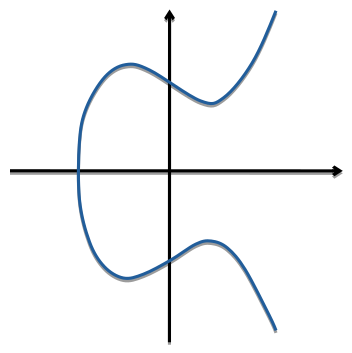
\includegraphics[width=\linewidth]{Assets/NetworkSecurity-ecc-1.png} 
            %      \item $y^2 = x^3-40x+5$ % 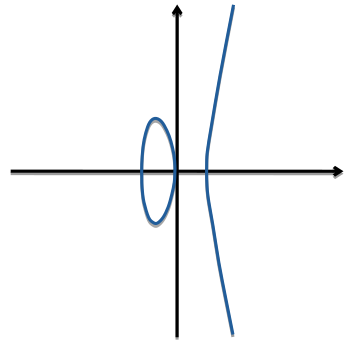
\includegraphics[width=\linewidth]{Assets/NetworkSecurity-ecc-2.png} 
            %\end{itemize*}
      \end{itemize*}

      \subsubsection{Punktaddition}
      \begin{itemize*}
            \item Addition von Elementen = Addition von Punkten auf der Kurve
            \item Geometrische Interpretation
            \begin{itemize*}
                  \item jeder Punkt $P:(x,y)$ hat einen Kehrwert $-P:(x,-y)$
                  \item eine Linie durch zwei Punkte $P$ und $Q$ schneidet sich normalerweise mit einem dritten Punkt $R$
                  \item die Summe von zwei Punkten $P$ und $Q$ ist $-R$
            \end{itemize*}
            \item Addition (Sonderfälle)
            \begin{itemize*}
                  \item Punkt $0$ ist das neutrale Element d.h. $P+O=P$
                  \item $P + (-P)=0$: wird der inverse Punkt zu P addiert, schneiden sich Linie und Kurve im ,,Unendlichen''
                  \item $P+P$: Die Summe zweier identischer Punkte $P$ ist der Kehrwert des Schnittpunkts mit der Tangente durch $P$
            \end{itemize*}
      \end{itemize*}
      \begin{center}
            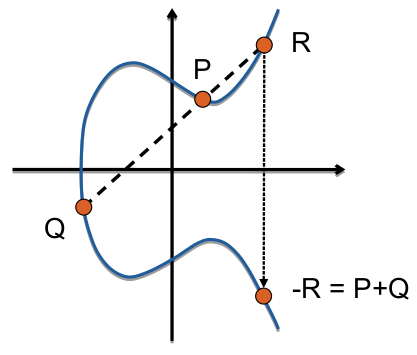
\includegraphics[width=.45\linewidth]{Assets/NetworkSecurity-ecc-3.png}
            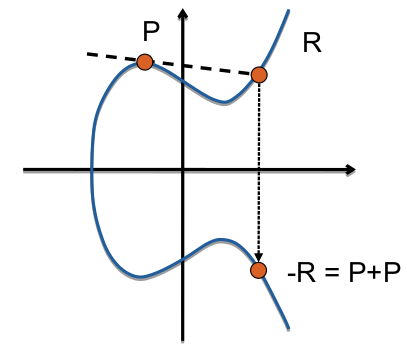
\includegraphics[width=.45\linewidth]{Assets/NetworkSecurity-ecc-4.png}
      \end{center}

      \subsubsection{Grundlagen des ECC - Algebraische Addition}
      \begin{itemize*}
            \item Wenn einer der Summanden $0$, ist die Summe der andere Summand
            \item Wenn die Summanden zueinander invers sind, ist die Summe $0$
            \item Für die allgemeineren Fälle ist die Steigung der Geraden: $\alpha=\begin{cases} \frac{y_Q-y_P}{x_Q-x_P} \quad\text{ for } P\not=-Q \vee P\not=Q \\ \frac{3x^2_P +a}{2y_P} \quad\text{ for } P=Q \end{cases}$
            \item Ergebnis der Punktaddition, wobei $(x_r,y_r)$ bereits der Spiegelpunkt $(-R)$ ist
      \end{itemize*}

      \subsubsection{Multiplikation}
      \begin{itemize*}
            \item Multiplikation von natürlicher Zahl $n$ und Punkt $P$ durch mehrfache wiederholte Additionen
            \item Zahlen werden in 2er-Potenzen gruppiert, um eine logarithmische Laufzeit zu erreichen, z.B. $25P = P + 8P + 16P$
            \item Dies ist nur möglich, wenn das $n$ bekannt ist
            \item Wenn $n$ für $nP=Q$ unbekannt ist, muss ein Logarithmus gelöst werden, wenn die Koordinatenwerte aus $\mathbb{R}$ gewählt werden
            \item Für $\mathbb{Z}_p$ und $GF(2^n)$ muss das diskrete Logarithmusproblem für elliptische Kurven gelöst werden, was nicht effizient durchgeführt werden kann!
            \item Hinweis: Es ist nicht definiert, wie zwei Punkte multipliziert werden, sondern nur eine natürliche Zahl $n$ und der Punkt $P$
      \end{itemize*}

      \subsubsection{Kurven über $\mathbb{Z}_p$}
      \begin{itemize*}
            \item Über $\mathbb{Z}_p$ zerfällt die Kurve in eine Menge von Punkten
            \item Für: $y^2=x^3-3x+5\ mod\ 19$
            \item 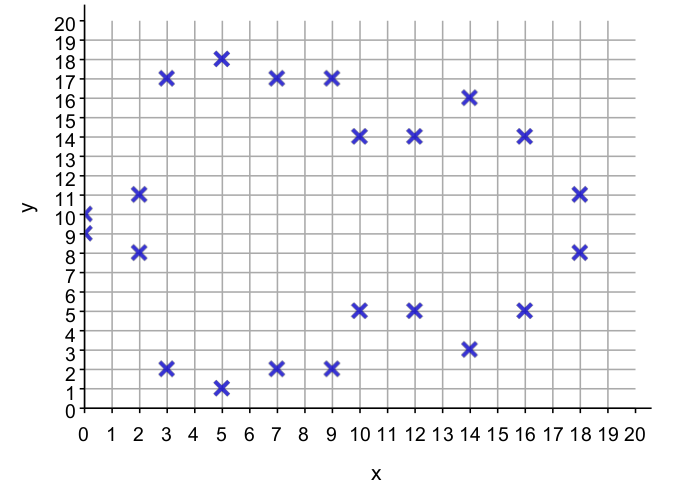
\includegraphics[width=.5\linewidth]{Assets/NetworkSecurity-ecc-5.png}
            \item Hinweis: Für einige x-Werte gibt es keinen y-Wert!
      \end{itemize*}

      \subsubsection{Berechnen Sie die y-Werte in $\mathbb{Z}_p$}
      \begin{itemize*}
            \item Im Allgemeinen etwas problematischer: Bestimmen Sie die y-Werte für ein gegebenes $x$ durch $y^2\equiv f(x)\ mod\ p$
            \item Daher wird $p$ oft s.t. gewählt $p\equiv 3\ mod\ 4$
            \item Dann wird y durch $y_1\equiv f(x)^{\frac{p+1}{4}}$ und $y_2\equiv -f(x)^{\frac{p+1}{4}}$ berechnet, wenn und nur wenn überhaupt eine Lösung existiert
            %\item Kurzer Beweis
            %\begin{itemize*}
            %      \item Aus dem Euler-Theorem 3 wissen wir, dass $f(x)^{p-1}\equiv 1\ mod\ p$
            %      \item Die Quadratwurzel muss also 1 oder -1 sein $f(x)^{\frac{p-1}{2}}\equiv\pm 1\ mod\ p$
            %\end{itemize*}
            %\item Fall 1: $f(x)^{\frac{p-1}{2}}\equiv1\ mod\ p$
            %\begin{itemize*}
            %      \item Multiplizieren Sie beide Seiten mit f(x): $f(x)^{\frac{p-1}{2}}\equiv f(x)\equiv y^2\ mod\ p$
            %      \item Da $p + 1$ durch 4 teilbar ist, können wir die Quadratwurzel ziehen, so dass $f(x)^{\frac{p-1}{2}}\equiv y\ mod\ p$
            %\end{itemize*}
            %\item Fall 2: In diesem Fall existiert keine Lösung für den gegebenen x-Wert (wie von Euler gezeigt)
      \end{itemize*}

      \subsubsection{Addition und Multiplikation in $\mathbb{Z}_p$}
      \begin{itemize*}
            \item Aufgrund des diskreten Strukturpunktes haben mathematische Operationen keine geometrische Interpretation mehr
            \item Algebraische Addition ähnlich der Addition über $\mathbb{R}$
            \item Wird der inverse Punkt zu $P$ addiert, schneiden sich Linie und ,,Kurve'' immer noch im ,,Unendlichen''
            \item Alle x- und y-Werte werden $mod\ p$ berechnet
            \item Division wird durch Multiplikation mit dem inversen Element des Nenners ersetzt
            \item Verwendung des erweiterten euklidischen Algorithmus mit $w$ und $p$ zur Ableitung der Inversen $-w$
            \item Die algebraische Multiplikation einer natürlichen Zahl $n$ und eines Punktes $P$ erfolgt ebenfalls durch wiederholte Addition von Summanden der Potenz von 2
            \item Das Problem des diskreten Logarithmus ist die Bestimmung einer natürlichen Zahl $n$ in $nP=Q$ für zwei bekannte Punkte $P$ und $Q$
      \end{itemize*}

      \subsubsection{ECC - Größe der erzeugten Gruppen}
      \begin{itemize*}
            \item beachte, dass die Ordnung einer durch einen Punkt auf einer Kurve über $\mathbb{Z}_p$ erzeugten Gruppe nicht $p-1$ ist
            \item Die Bestimmung der exakten Ordnung ist nicht einfach, kann aber mit Schoofs Algorithmus in logarithmischer Zeit durchgeführt werden %(erfordert viel mehr mathematischen Hintergrund als hier gewünscht)
            \item Satz von Hasse über elliptische Kurven besagt, dass die Gruppengröße $n$ zwischen: $p+1 - 2\sqrt{p}\leq n\leq p+1+2\sqrt{p}$ liegen muss
            \item Es genügt, relativ große Gruppen zu erzeugen
      \end{itemize*}

      \subsubsection{ECDH - ECC Diffie Hellmann}
      \begin{itemize*}
            \item Diffie-Hellman kann leicht an elliptische Kurven angepasst werden
            \item Wenn A und B sich auf ein gemeinsames Geheimnis $s$ einigen wollen
            \begin{itemize*}
                  \item A und B einigen sich auf eine kryptographisch sichere elliptische Kurve und einen Punkt $P$ auf dieser Kurve
                  \item A wählt eine Zufallszahl $q$: A berechnet $Q=qP$ und überträgt $Q$ an B
                  \item B wählt eine Zufallszahl $r$: B berechnet $R=rP$ und überträgt $P$ an A
                  \item Beide Seiten errechnen das gemeinsame Geheimnis: A errechnet $S=qR$, B errechnet $S'=rQ$
                  \item da $qrP=rqP \rightarrow$ der geheime Punkt $S=S'$
            \end{itemize*}
            \item Angreifer, die den öffentlichen Kanal abhören, können $S$ nur berechnen, wenn sie entweder $q$ oder $r$ berechnen können, die die diskreten Logarithmen von $Q$ und $R$ für den Punkt $P$ sind
      \end{itemize*}

      \subsubsection{EC-Version des ElGamal-Algorithmus}
      \begin{itemize*}
            \item Anpassung von ElGamal für elliptische Kurven% ist für die Verschlüsselungsroutine recht einfach
            \item Schlüsselpaar einrichten
            \begin{itemize*}
                  \item Wählen eine elliptische Kurve über einem endlichen Feld, einen Punkt $G$, der eine große Gruppe erzeugt, und eine Zufallszahl $v$, so dass $1 < v < n$, wobei $n$ die Größe der induzierten Gruppe bezeichnet. Berechne: $Y = vG$
                  \item Der öffentliche Schlüssel ist $(Y,G,Kurve)$
                  \item Der private Schlüssel ist $v$
            \end{itemize*}
            \item Nachricht verschlüsseln
            \begin{itemize*}
                  \item Wähle zufälliges $k\in\mathbb{Z}^+$ mit $k<n-1$, berechne $R=kG$
                  \item Berechne $S=M+kY$, wobei $M$ ein von der Nachricht abgeleiteter Punkt ist
                  \item Problem: Die Interpretation der Nachricht $m$ als x-Koordinate von $M$ ist nicht ausreichend, da der y-Wert nicht existieren muss
                  \item Lösung: Wähle eine Konstante $c$ und prüfe, ob $cm$ die x-Koordinate eines gültigen Punktes ist, wenn nicht, versuche $cm+1$, dann $cm+2$ usw.
                  \item Um m zu entschlüsseln: nimm den x-Wert von M und führe eine ganzzahlige Division durch $c$ durch (der Empfänger muss c ebenfalls kennen)
                  \item Der Chiffretext sind die Punkte $(R,S)$
                  \item Doppelt so lang wie $m$, wenn sie in so genannter komprimierter Form gespeichert werden, d.h. nur die x-Koordinaten werden gespeichert und ein einziges Bit, das angibt, ob die größere oder kleinere entsprechende y-Koordinate verwendet werden soll
            \end{itemize*}
            \item Nachricht entschlüsseln
            \begin{itemize*}
                  \item Ableitung von M durch Berechnung von $S-vR$
                  \item Beweis: $S-vR=M+kY-vR =M+kvG-vkG= M+O= M$
            \end{itemize*}
            \item Nachricht signieren
            \begin{itemize*}
                  \item Wähle zufälliges $k\in\mathbb{Z}^+$ mit $k<n-1$, berechne $R=kG$
                  \item Berechne $s=k^{-1}(m+rv) mod\ n$, wobei $r$ der x-Wert von R
                  \item Die Signatur ist $(r,s)$, wiederum etwa doppelt so lang wie $n$
            \end{itemize*}
            \item Überprüfen einer signierten Nachricht
            \begin{itemize*}
                  \item Prüfen, ob der Punkt $P=ms^{-1}G+rs^{-1}Y$ die x-Koordinate $r$ hat
                  \item Anmerkung: $s^{-1}$ wird durch den Erweiterten Euklidischen Algorithmus mit den Eingaben $s$ und $n$ berechnet
                  \item Beweis: $ms^{-1}G+rs^{-1}Y = ms^{-1}G+rs^{-1}vG = (m+rv)(s^{-1})G = (ks)(s^{-1})G = kG = R$
            \end{itemize*}
            \item Diskussion zur Sicherheit
            \begin{itemize*}
                  \item Wie in der ursprünglichen Version von ElGamal ist es entscheidend, $k$ nicht zweimal zu verwenden
                  \item Nachrichten sollten nicht direkt signiert werden
                  \item Weitere Prüfungen können erforderlich sein, d.h. $G$ darf nicht $0$ sein, ein gültiger Punkt auf der Kurve usw.
            \end{itemize*}
      \end{itemize*}

      \subsubsection{Sicherheit}
      \begin{itemize*}
            \item Die Sicherheit hängt stark von der gewählten Kurve und dem Punkt ab:
            \item Die Diskriminante der Kurve darf nicht Null sein, d.h. $4a^3+27b^2\not\equiv 0\ mod\ p$ sonst ist die Kurve degradiert %(eine sogenannte ,,singuläre Kurve'' )
            \item Menezes haben einen subexponentiellen Algorithmus für sogenannte ,,supersinguläre elliptische Kurven'' gefunden, der aber im allgemeinen Fall nicht funktioniert
            \item Die konstruierten algebraischen Gruppen sollten so viele Elemente wie möglich haben
            \item Viele Veröffentlichungen wählen die Parameter a und b so, dass sie nachweislich durch einen Zufallsprozess gewählt werden; so soll sichergestellt werden, dass die Kurven keine kryptographische Schwäche enthalten, die nur den Autoren bekannt ist
            \item Die Sicherheit ist abhängig von der Länge von $p$
            \begin{tabular}{c|c|c}
                  Symmetrische A. & RSA   & ECC     \\\hline
                  112             & 2048  & 224-255 \\
                  128             & 3072  & 256-383 \\
                  192             & 7680  & 384-511 \\
                  256             & 15360 & $>$512
            \end{tabular}
            \item Die Sicherheit hängt auch stark von der Implementierung ab
            \begin{itemize*}
                  \item Die verschiedenen Fälle in der ECC-Berechnung können beobachtbar sein, d.h. Stromverbrauch und Zeitunterschiede
                  \item Angreifer können Seitenkanalangriffe ableiten%, wie in OpenSSL 0.9.8
                  \item Ein Angreifer kann die Bitlänge eines Wertes $k$ in $kP$ ableiten, indem er die für den Quadrat- und Multiplikationsalgorithmus benötigte Zeit misst
                  \item Der Algorithmus wurde in OpenSSL frühzeitig abgebrochen, wenn keine weiteren Bits auf ,,1'' gesetzt wurden
                  \item Angreifer könnten versuchen, ungültige Punkte zu generieren, um Fakten über den verwendeten Schlüssel abzuleiten was zu einer Wiederherstellung eines vollen 256-Bit ECC-Schlüssels nach nur 633 Abfragen führte
            \end{itemize*}
            \item Lektion gelernt: Machen Sie es nicht selbst, es sei denn, Sie müssen es tun und wissen, was Sie tun
      \end{itemize*}

      \subsubsection{Weitere Anmerkungen}
      \begin{itemize*}
            \item es ist möglich, kryptographische elliptische Kurven über $G(2^n)$ zu konstruieren, was in Hardware-Implementierungen schneller sein kann
            \item Elliptische Kurven und ähnliche algebraische Gruppen sind ein aktives Forschungsgebiet und ermöglichen weitere fortgeschrittene Anwendungen
            \begin{itemize*}
                  \item Edwards-Kurven scheinen robuster gegen Seitenkanalangriffe
                  \item Bilineare Paarungen ermöglichen
                  \item Programme zu verifizieren, dass sie zur selben Gruppe gehören, ohne ihre Identität preiszugeben
                  \item Öffentliche Schlüssel können strukturiert werden%, z.B. ,,Alice'' als öffentlicher Schlüssel für Alice verwenden
            \end{itemize*}
      \end{itemize*}

      \subsection{Schlussfolgerung}
      \begin{itemize*}
            \item Asymmetrische Kryptographie erlaubt es, zwei verschiedene Schlüssel zu verwenden
            \begin{itemize*}
                  \item Verschlüsselung / Entschlüsselung
                  \item Signieren / Überprüfen
            \end{itemize*}
            \item die praktischsten Algorithmen, die immer noch als sicher gelten
            \begin{description*}
                  \item[RSA] diskrete Logarithmen faktorisieren und lösen
                  \item[Diffie-Hellman] Schlüsselvereinbarungsprotokoll
                  \item[ElGamal] wie DH basierend auf diskreten Logarithmen
            \end{description*}
            \item Da ihre Sicherheit vollständig auf der Schwierigkeit bestimmter mathematischer Probleme beruht, stellt der algorithmische Fortschritt ihre größte Bedrohung dar
            \item Praktische Überlegungen:
            \begin{itemize*}
                  \item Asymmetrische kryptografische Operationen sind um Größenordnungen langsamer als symmetrische Operationen
                  \item Daher werden sie oft nicht für die Verschlüsselung/Signierung von Massendaten verwendet
                  \item Symmetrische Verfahren werden zur Verschlüsselung / Berechnung eines kryptografischen Hashwerts verwendet, während die asymmetrische Kryptografie nur zur Verschlüsselung eines Schlüssels / Hashwerts eingesetzt wird
            \end{itemize*}
      \end{itemize*}

      \columnbreak

      \section{Modifikationsprüfwerte}
      \begin{itemize*}
            \item In Kommunikation üblich, eine Art Fehlererkennungscode für Nachrichten zu berechnen, mit dem Empfänger überprüfen können, ob eine Nachricht während der Übertragung verändert wurde.
            \item Bsp: Parität, Bit-Interleaved Parity, Cyclic Redundancy Check
            \item Dies führt zu dem Wunsch, einen ähnlichen Wert zu haben, der es ermöglicht zu überprüfen, ob eine Nachricht während der Übertragung verändert wurde.
            \item großer Unterschied, ob man davon ausgeht, dass die Nachricht durch zufällige Fehler oder absichtlich verändert wird
            \item Wenn jemand eine Nachricht, die mit einem CRC-Wert geschützt ist, absichtlich verändern will, kann er den CRC-Wert nach der Veränderung neu berechnen oder die Nachricht so verändern, dass sie den gleichen CRC-Wert ergibt
            \item Ein Änderungsprüfwert muss also einige zusätzliche Eigenschaften erfüllen, die es Angreifern unmöglich machen, ihn zu fälschen
            \item Zwei Hauptkategorien von Modifikationsprüfwerten
            \begin{itemize*}
                  \item Modifikationserkennungscode (MDC)
                  \item Nachrichten-Authentifizierungs-Code (MAC)
            \end{itemize*}
      \end{itemize*}

      \subsection{Kryptographische Hash-Funktionen}
      \begin{itemize*}
            \item Definition: Hash-Funktion ist eine Funktion $h$ mit folgenden zwei Eigenschaften
            \begin{description*}
                  \item[Komprimierung] $h$ bildet eine Eingabe $x$ mit beliebiger endlicher Bitlänge auf eine Ausgabe $h(x)$ mit fester Bitlänge $n$ ab
                  \item[Einfachheit] der Berechnung: Bei $h$ und $x$ ist es einfach, $h(x)$ zu berechnen
            \end{description*}
            \item Definition: kryptografische Hash-Funktion, ist eine Hash-Funktion, die zusätzlich folgende Eigenschaften erfüllt
            \begin{description*}
                  \item[Pre-Image-Resistenz] für im Wesentlichen alle vorgegebenen Ausgaben $y$ ist es rechnerisch nicht möglich, ein $x$ zu finden, so dass $h(x)=y$
                  \item[Vorabbild-Resistenz] Bei $x$ ist es rechnerisch nicht möglich, eine zweite Eingabe $x'$ mit $x\not= x'$ zu finden, so dass $h(x)=h(x')$
                  \item[Kollisionssicherheit] Es ist rechnerisch nicht möglich, ein beliebiges Paar $(x,x')$ mit $x\not= x'$ zu finden, so dass $h(x)=h(x')$
            \end{description*}
            \item Kryptographische Hash-Funktionen werden zur Berechnung von Modification Detection Codes (MDC) verwendet
      \end{itemize*}

      \subsection{Nachrichten-Authentifizierungs-Codes (MAC)}
      \begin{itemize*}
            \item ist eine Familie von Funktionen $h_k$, die durch einen geheimen Schlüssel $k$ parametrisiert sind und die folgenden Eigenschaften aufweisen
            \begin{description*}
                  \item[Komprimierung] $hk$ bildet eine Eingabe $x$ beliebiger endlicher Bitlänge auf eine Ausgabe $h_k(x)$ fester Bitlänge ab, genannt MAC
                  \item[Einfache Berechnung] Bei $k$, $x$ und einer bekannten Funktionsfamilie $h_k$ ist der Wert $h_k(x)$ einfach zu berechnen
                  \item[Berechnungsresistenz] für jeden festen, erlaubten, aber unbekannten Wert von $k$ ist es bei null oder mehr Text-MAC-Paaren $(x_i, h_k(x_i))$ rechnerisch nicht möglich, ein Text-MAC-Paar $(x, h_k(x))$ für jede neue Eingabe $x\not= x_i$ zu berechnen
            \end{description*}
            \item Bitte beachten Sie, dass Rechenresistenz die Eigenschaft der Nicht-Wiederherstellung des Schlüssels impliziert, d.h. k kann nicht aus Paaren $(x_i,h_k(x_i))$ wiederhergestellt werden, aber Rechenresistenz kann nicht aus der Nicht-Wiederherstellung des Schlüssels abgeleitet werden, da der Schlüssel $k$ nicht immer wiederhergestellt werden muss, um neue MACs zu fälschen
      \end{itemize*}

      \subsection{einfacher Angriff gegen unsicheren MAC}
      \begin{itemize*}
            \item zur Veranschaulichung folgende MAC-Definition
            \begin{itemize*}
                  \item Eingabe: Nachricht $m=(x_1,x_2,...,x_n)$, wobei $x_i$ 64-Bit-Werte sind, und Schlüssel $k$
                  \item Berechne $\delta(m):= x_1\oplus x_2\oplus...\oplus x_n$, wobei $\oplus$ die bitweise Exklusiv-Oder-Verknüpfung bezeichnet
                  \item Ausgabe: MAC $C_k(m):= E_k(\delta(m))$ mit $E_k(x)$ für die DES-Verschlüsselung
            \end{itemize*}
            \item Die Schlüssellänge beträgt 56 Bit und die MAC-Länge 64 Bit, so dass wir einen Aufwand von etwa $2^{55}$ Operationen erwarten würden, um den Schlüssel $k$ zu erhalten und den MAC zu knacken %(= Nachrichten fälschen zu können).
            \item Leider ist die MAC-Definition unsicher
            \begin{itemize*}
                  \item Angenommen, ein Angreifer E, der die zwischen A und B ausgetauschten Nachrichten fälschen will, erhält eine Nachricht $(m,C_k(m))$, die von Alice mit dem mit Bob geteilten geheimen Schlüssel $k$ ,,geschützt'' wurde
                  \item Eve kann eine Nachricht $m'$ konstruieren, die denselben MAC ergibt
                  \item Sei $y_1,y_2,...,y_{n-1}$ ein beliebiger 64-Bit-Wert
                  \item Definiere $y_n:= y_1\oplus y_2\oplus...\oplus y_{n-1}\oplus \delta(m)$ und $m':=(y_1,y_2,...,y_n)$
                  \item Wenn B $(m',C_k(m))$ von E erhält, die vorgibt, A zu sein, wird er es als von A stammend akzeptieren, da $C_k(m)$ ein gültiger MAC für $m'$ ist
            \end{itemize*}
      \end{itemize*}

      \subsection{Anwendungen für Hash-Funktionen und MACs}
      \begin{itemize*}
            \item Integrität von Nachrichten
            \begin{itemize*}
                  \item MDC stellt digitalen Fingerabdruck dar, der mit einem privaten Schlüssel signiert werden kann und es ist nicht möglich, zwei Nachrichten mit demselben Fingerabdruck zu erstellen%, so dass ein bestimmter signierter Fingerabdruck von einem Angreifer nicht wiederverwendet werden kann
                  \item MAC über Nachricht $m$ bescheinigt direkt, dass der Absender der Nachricht im Besitz des geheimen Schlüssels $k$ ist und die Nachricht ohne Kenntnis dieses Schlüssels nicht verändert worden sein kann
            \end{itemize*}
            \item Bestätigung von Wissen
            \item Schlüsselableitung
            \item Pseudo-Zufallszahlengenerierung
            \item Je nach Anwendung weitere Anforderungen
            \begin{itemize*}
                  \item Partielle Vorabbild-Resistenz: auch wenn nur ein Teil der Eingabe, z.B. t Bit, unbekannt ist, sollte es im Durchschnitt $2^{t-1}$ Operationen benötigen, um diese Bits zu finden
            \end{itemize*}
      \end{itemize*}

      \subsection{Angriffe basierend auf dem Geburtstagsphänomen}
      \begin{itemize*}
            \item Geburtstagsphänomen: Wie viele Personen müssen sich in einem Raum befinden, damit die Wahrscheinlichkeit, dass es mindestens zwei Personen mit demselben Geburtstag gibt, größer als $0,5$ ist?
            \item Definiere $P(n,k):= Pr$,,mindestens ein Duplikat in $k$ Elementen, wobei jedes Element einen von $n$ gleich wahrscheinlichen Werten zwischen 1 und $n$ annehmen kann ''
            \item Definiere $Q(n,k):= Pr$,,kein Duplikat in $k$ Artikeln, jeder Artikel zwischen 1 und $n$''
            \begin{itemize*}
                  \item das erste Element aus $n$ möglichen Werten wählen, das zweite Element aus $n-1$ möglichen Werten, usw.
                  \item Die Anzahl der verschiedenen Möglichkeiten, $k$ Elemente aus $n$ Werten ohne Duplikate auszuwählen, ist also: $N=n \times (n-1)\times ...\times (n-k+1)= n!\backslash(n-k)!$
                  \item Die Anzahl der verschiedenen Möglichkeiten, $k$ Elemente aus $n$ Werten auszuwählen, mit oder ohne Duplikate, ist $n^k$
                  \item Also, $Q(n,k)=N\backslash n^k=n!\backslash((n-k)! \times n^k)$
            \end{itemize*}
            \item Wir haben: $P(n,k)=1-Q(n,k)=1-\frac{n!}{(n-k)!\times n^k}$ %$=1-\frac{n\times(n-1)\times...\times(n-k+1)}{n^k}=1-,,(1-\frac{1}{n})\times(1-\frac{2}{n})\times...\times(1-\frac{k-1}{n})''$
            \item folgende Ungleichung $(1-x) \leq e^{-x}$ für alle $x \geq 0$
            \item So: $P(n,k)>1-e^{\frac{-k\times(k-1)}{2n}}$ %$=1-[(e^{-1/n})\times(e^{-2/n})\times...\times(e^{-(k-1)/n})]$
            \item Im letzten Schritt: $1+2+...+(k-1)=(k^2 - k)\backslash 2$
            \item Geburtstagsphänomen: $n=365$ mit Wahrscheinlichkeit $\geq 0,5$?
            \begin{itemize*}
                  \item $\frac{1}{2}=1-e^{\frac{-k\times(k-1)}{2n}}\Leftrightarrow 2=e^{\frac{k\times(k-1)}{2n}}\Leftrightarrow ln(2)=\frac{k\times(k-1)}{2n}$
                  \item für große $k$ kann $k\times(k-1)$ durch $k^2$ approximiert werden und erhalten: $k=\sqrt{2 ln(2)n}\approx 1,18\sqrt{n}$
                  \item für $n=365$ wird $k=22,54$%, was der richtigen Antwort recht nahe kommt 23
            \end{itemize*}
            \item bei $n$ möglichen unterschiedlichen Werten liegt die Anzahl $k$ der Werte, die man zufällig wählen muss, um mindestens ein Paar identischer Werte zu erhalten, in der Größenordnung von $\sqrt{n}$
            \item Betrachten folgenden Angriff
            \begin{itemize*}
                  \item E möchte, dass A eine Nachricht $m1$ signiert, die A normalerweise nie signieren würde. E weiß, dass A die Funktion $MDC1(m)$ verwendet, um eine MDC von $m$ zu berechnen, die eine Länge von $r$ Bit hat, bevor sie diese MDC mit ihrem privaten Schlüssel signiert, was ihre digitale Signatur ergibt
                  \item Zunächst erzeugt E ihre Nachricht $m1$. Würde sie nun $MDC1(m1)$ berechnen und dann versuchen, eine zweite harmlose Nachricht $m2$ zu finden, die zu demselben MDC führt, wäre ihr Suchaufwand im durchschnittlichen Fall in der Größenordnung von $2^{(r-1)}$
                  \item Stattdessen nimmt sie eine beliebige harmlose Nachricht $m2$ und beginnt, Variationen $m1'$ und $m2'$ der beiden Nachrichten zu produzieren%, z.B. durch Hinzufügen von -Kombinationen oder Variationen mit semantisch identischen Wörtern.
            \end{itemize*}
            \item E muss nur etwa $\sqrt{2^r}=2^{r/2}$ Variationen von jeder der beiden Nachrichten produzieren, so dass die Wahrscheinlichkeit, dass sie zwei Nachrichten $m1'$ und $m2'$ mit demselben MDC erhält, mindestens $0,5$ beträgt
            \item Da sie die Nachrichten zusammen mit ihren MDCs speichern muss, um eine Übereinstimmung zu finden, liegt der Speicherbedarf ihres Angriffs in der Größenordnung von $2^{\frac{r}{2}}$ und der Rechenzeitbedarf in der gleichen Größenordnung
            \item Nachdem sie $m1'$ und $m2'$ mit $MDC1(m1')=MDC1(m2')$ gefunden hat, fordert sie A auf, $m2'$ zu signieren. E kann dann diese Unterschrift nehmen und behaupten, dass A $m1'$ unterschrieben hat
            \item diese Methode wird Geburtstagsangriff genannt
            \item Bsp: A nutzt RSA mit $2048$Bit Schlüsseln und kryptographische Hashfunktion mit $96$Bit Länge. E durchschnittlicher Aufwand, zwei Nachrichten $m1'$ und $m2'$ zu erzeugen, liegt in Größenordnung $2^{48}$ (heute machbar) %Das Knacken von RSA-Schlüsseln der Länge 2048 Bit ist mit den heutigen Algorithmen und Technologien bei weitem nicht möglich.
      \end{itemize*}

      \subsection{Übersicht über die gebräuchlichen MDCs}
      \begin{itemize*}
            \item Kryptografische Hash-Funktionen zur Erstellung von MDCs
            \begin{description*}
                  \item[Message Digest 5] (MD5)  Erfunden von R. Rivest
                  \item[Sicherer Hash-Algorithmus 1] (SHA-1) von NSA
                  \item[Sicherer Hash-Algorithmus 2] (SHA-2, SHA-256, SHA-512)
                  \begin{itemize*}
                        \item Größere Blockgröße \& komplexere Rundenfunktion
                  \end{itemize*}
                  \item[Sicherer Hash-Algorithmus 3] (SHA-3, Keccak)
                  \begin{itemize*}
                        \item Gewinner eines offenen Wettbewerbs
                        \item Sogenannte Sponge-Konstruktion
                        \item Vielseitiger als frühere Hash-Funktionen
                  \end{itemize*}
            \end{description*}
            \item Nachrichten-Authentifizierungs-Codes (MACs)
            \begin{itemize*}
                  \item DES-CBC-MAC
                  \begin{itemize*}
                        \item Verwendet den Data Encryption Standard im Cipher Block Chaining Modus
                        \item allgemein kann CBC-MAC-Konstruktion mit jeder Blockchiffre verwendet werden
                  \end{itemize*}
                  \item MACs, die aus MDCs aufgebaut sind (sehr verbreitet)
                  %\begin{itemize*}
                  %      \item Dieser sehr verbreitete Ansatz wirft einige kryptografische Bedenken auf, da er einige implizite, aber nicht verifizierte Annahmen über die Eigenschaften der MDCs trifft.
                  %\end{itemize*}
            \end{itemize*}
            \item Authentifizierte Verschlüsselung mit zugehörigen Daten (AEAD)
            \begin{description*}
                  \item[Galois-Counter-Verfahren] (GCM) Verwendet eine Blockchiffre zur Verschlüsselung und Authentifizierung von Daten
                  \item[Sponge Wrap] Verwendet eine SHA-3 ähnliche Hash-Funktion zur Verschlüsselung und Authentifizierung von Daten
            \end{description*}
      \end{itemize*}

      \subsection{Struktur von kryp. Hash-Funktionen}
      \begin{itemize*}
            \item viele der heute verwendeten kryptografischen Hash-Funktionen folgen einer gemeinsamen Struktur, der sogenannten Merkle-Dåmgard-Struktur
            \begin{itemize*}
                  \item Sei $y$ eine beliebige Nachricht. Normalerweise wird die Länge der Nachricht an die Nachricht angehängt und auf ein Vielfaches einer Blockgröße $b$ aufgefüllt. Bezeichnen wir $(y_0,y_1,...,y_{L-1})$ die resultierende Nachricht, die aus $L$ Blöcken der Größe $b$
                  \item Die allgemeine Struktur ist wie folgt abgebildet: 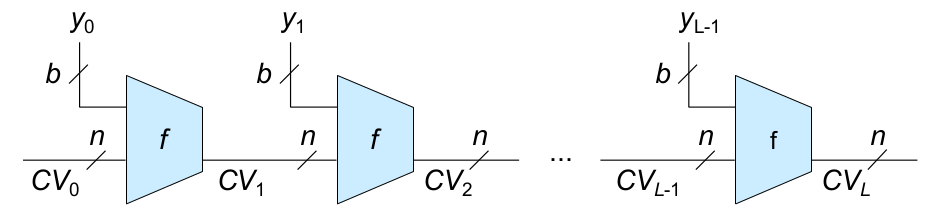
\includegraphics[width=.5\linewidth]{Assets/NetworkSecurity-feistel.png}
                  \item $CV$ ist Verkettungswert mit $CV_0:=IV$ und $MDC(y):=CV_L$
                  \item $f$ ist spezifische Kompressionsfunktion, die $(n+b)$ Bit auf $n$ Bit komprimiert
            \end{itemize*}
            \item Die Hash-Funktion H lässt sich wie folgt zusammenfassen:
            \begin{itemize*}
                  \item $CV_0 = IV =$ anfänglicher n-Bit-Wert
                  \item $CV_i = f(CV_{i -1}, y_{i-1}) \quad\quad 1\leq i \leq L$
                  \item $H(y) = CV_L$
            \end{itemize*}
            \item Es wurde gezeigt, dass, wenn die Kompressionsfunktion $f$ kollisionssicher ist, die resultierende iterierte Hash-Funktion $H$ ebenfalls kollisionssicher ist
            \item Kryptoanalyse krypt. Hash-Funktionen konzentriert sich auf interne Struktur der Funktion $f$ und Suche nach effizienten Techniken zur Erzeugung von Kollisionen bei einer einzigen Ausführung von $f$
            \item gängiger Mindestvorschlag für $n$, die Bitlänge des Hashwerts, $160$Bit, da dies einen Aufwand der Größenordnung $2^{80}$ für einen Angriff impliziert, der heute als undurchführbar gilt
      \end{itemize*}

      \subsection{Der Message Digest 5}
      \begin{itemize*}
            \item MD5 folgt der zuvor skizzierten allgemeinen Struktur
            \item Nachricht $y$ wird mit einer ,,1'' aufgefüllt, gefolgt von 0 bis 511 ,,0'' Bits, so dass die Länge der resultierenden Nachricht kongruent $448\ mod\ 512$ ist
            \item Länge der ursprünglichen Nachricht wird als $64$Bit-Wert hinzugefügt, so dass eine Nachricht entsteht, deren Länge ein ganzzahliges Vielfaches von $512$Bit ist
            \item diese neue Nachricht wird in Blöcke der Länge $b=512$Bit unterteilt.
            \item die Länge des Verkettungswertes ist $n=128$Bit
            \item Verkettungswert ist strukturiert als vier 32-Bit-Register A,B,C,D
            \item Initialisierung
            \begin{itemize*}
                  \item A := 0x 01 23 45 67,$\quad$ B := 0x 89 AB CD EF
                  \item C := 0x FE DC BA 98,$\quad$ D := 0x 76 54 32 10
            \end{itemize*}
            \item Jeder Block der Nachricht $y_i$ wird mit dem Verkettungswert $CV_i$ mit der Funktion f verarbeitet, die intern durch 4 Runden zu je 16 Schritten realisiert ist
            \begin{itemize*}
                  \item Jede Runde ist ähnlich aufgebaut und verwendet eine Tabelle $T$, die 64 konstante Werte von je 32 Bit enthält,
                  \item Jede der vier Runden verwendet eine bestimmte logische Funktion g
            \end{itemize*}
            \item 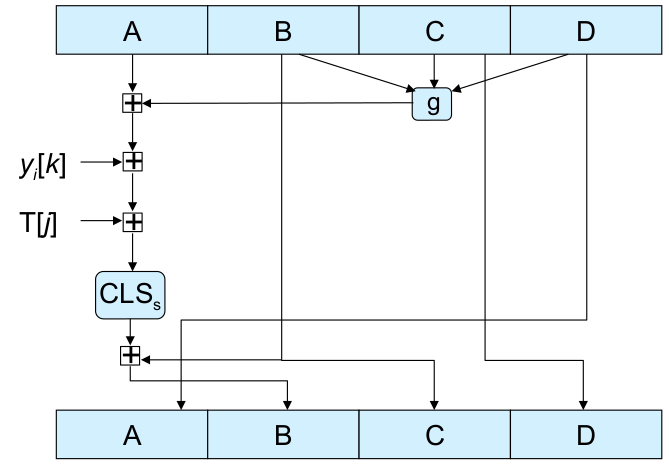
\includegraphics[width=.4\linewidth]{Assets/NetworkSecurity-md5.png}
            \item Die Funktion g ist eine von vier verschiedenen logischen Funktionen
            \item $y_i,,k''$ bezeichnet das k-te $32$Bit-Wort des Nachrichtenblocks $i$
            \item $T[j]$ ist der j-te Eintrag der Tabelle $t$, wobei $j$ bei jedem Schritt $mod\ 64$ inkrementiert wird
            \item CLS s bezeichnet die zyklische Linksverschiebung um $s$ Bits, wobei $s$ einem bestimmten Schema folgt
            \item Der MD5-MDC über eine Nachricht ist der Inhalt des Verkettungswertes CV nach Verarbeitung des letzten Nachrichtenblocks
            \item Sicherheit von MD5
            \begin{itemize*}
                  \item Jedes Bit des $128$Bit-Hash-Codes ist eine Funktion eines jeden Eingabebits
                  \item 1996 veröffentlichte H. Dobbertin einen Angriff, der es erlaubt, eine Kollision für die Funktion f zu erzeugen %(realisiert durch die oben beschriebenen 64 Schritte).
                  \item dauerte bis 2004 bis eine erste Kollision gefunden wurde
                  \item Inzwischen möglich Kollisionen innerhalb von Sekunden auf allgemeiner Hardware zu erzeugen
                  \item MD5 darf nicht in Betracht gezogen werden, wenn Kollisionssicherheit erforderlich ist
                  \item Die Resistenz gegen Preimage-Angriffe ist mit $2123.4$ Berechnungen noch ok
            \end{itemize*}
      \end{itemize*}

      \subsection{Der sichere Hash-Algorithmus SHA-1}
      \begin{itemize*}
            \item Auch SHA-1 folgt der gleichen Struktur wie oben
            \item SHA-1 arbeitet mit $512$Bit-Blöcken und erzeugt einen $160$Bit-Hash-Wert
            \item Design vom MD4-Algorithmus inspiriert, Initialisierung im Grunde dieselbe wie MD5
            \begin{itemize*}
                  \item Die Daten werden aufgefüllt, ein Längenfeld wird hinzugefügt und die resultierende Nachricht wird als Blöcke der Länge $512$Bit verarbeitet
                  \item Verkettungswert als fünf $32$Bit-Register A,B,C,D,E
                  \item Initialisierung
                  \begin{itemize*}
                        \item A = 0x 67 45 23 01, $\quad$ B = 0x EF CD AB 89
                        \item C = 0x 98 BA DC FE, $\quad$ D = 0x 10 32 54 76
                        \item E = 0x C3 D2 E1 F0
                  \end{itemize*}
                  \item Die Werte werden im Big-Endian-Format gespeichert
            \end{itemize*}
            \item Jeder Block $y_i$ der Nachricht wird zusammen mit $CV_i$ in einem Modul verarbeitet, das die Kompressionsfunktion $f$ in vier Runden zu je 20 Schritten realisiert
            \begin{itemize*}
                  \item Runden haben ähnliche Struktur, aber jede Runde verwendet eine andere primitive logische Funktion $f_1, f_2, f_3, f_4$
                  \item Bei jedem Schritt wird eine feste additive Konstante $K_t$ verwendet, die während einer Runde unverändert bleibt
            \end{itemize*}
            \item 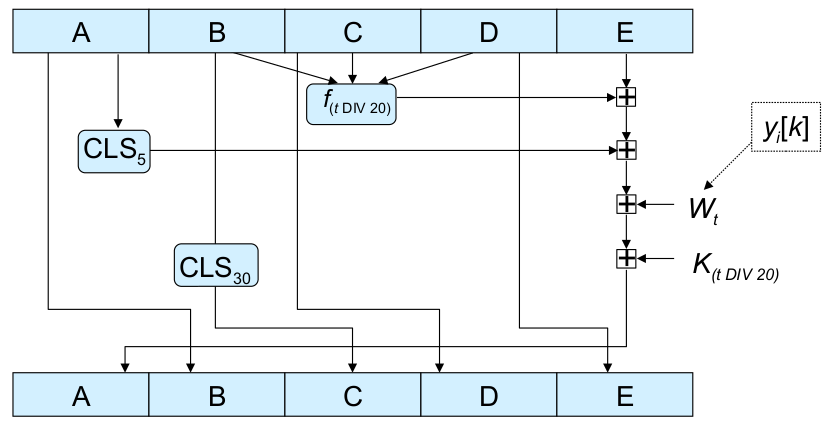
\includegraphics[width=.5\linewidth]{Assets/NetworkSecurity-sha1.png}
            \begin{itemize*}
                  \item $t\in{0,...,15}\Rightarrow W_t:= y_i,,t''$
                  \item $t\in{16,...,79}\Rightarrow W_t:=CLS_1(W_{t-16}\oplus W_{t-14}\oplus W_{t-8} \oplus W_{t-3})$
                  \item Nach Schritt 79 wird jedes Register A,B,C,D,E modulo $2^{32}$ mit dem Wert des entsprechenden Registers vor Schritt 0 addiert, um $CV_{i+1}$ zu berechnen
            \end{itemize*}
            \item SHA-1-MDC über Nachricht ist Inhalt des Verkettungswertes CV nach Verarbeitung des letzten Nachrichtenblocks
            \item Vergleich zwischen SHA-1 und MD5
            \begin{itemize*}
                  \item Geschwindigkeit: SHA-1 ist etwa 25\% langsamer als MD5 %(CV ist etwa 25\% größer)
                  \item Einfachheit und Kompaktheit: beide Algorithmen einfach zu beschreiben und zu implementieren und erfordern keine großen Programme oder Ersetzungstabellen
            \end{itemize*}
            \item Sicherheit von SHA-1
            \begin{itemize*}
                  \item SHA-1 MDCs der Länge 160 Bit, bessere Sicherheit gegen Brute-Force- und Geburtstagsangriffe erwartet als MD5
                  \item Einige inhärente Schwächen von Merkle-Dåmgard-Konstruktionen sind vorhanden
                  \item Im Februar 2005 veröffentlichten X. Wang et. al. einen Angriff, der es erlaubt, eine Kollision mit einem Aufwand von $2^{69}$ zu finden, der in den folgenden Monaten auf $2^{63}$ verbessert wurde
                  \item Die Forschung ging weiter und im Februar 2017 wurde die erste tatsächliche Kollision gefunden %(demonstriert mit einem veränderten PDF-Dokument)
            \end{itemize*}
            \item SHA-2-Familie
            \begin{itemize*}
                  \item 2001 veröffentlichte das NIST neuen Standard FIPS PUB 180-2 mit Bezeichnungen SHA-256, SHA-384 und SHA-512 mit 256, 384 und 512 Bits
                  \item SHA-224 wurde 2004 hinzugefügt
                  \item SHA-224 und SHA-384 sind verkürzte Versionen von SHA-256 und SHA-512 mit unterschiedlichen Initialisierungswerten
                  \item SHA-2 verwendet ebenfalls die Merkle-Dåmgard-Konstruktion mit einer Blockgröße von 512 Bit (SHA-256) und 1024 Bit (SHA-512)
                  \item Der interne Zustand ist in 8 Registern von 32 Bit (SHA-256) und 64 Bit (SHA-512) organisiert
                  \item 64 Runden (SHA-256) oder 80 Runden (SHA-512)
                  \item Ein Schritt
                  \begin{itemize*}
                        \item 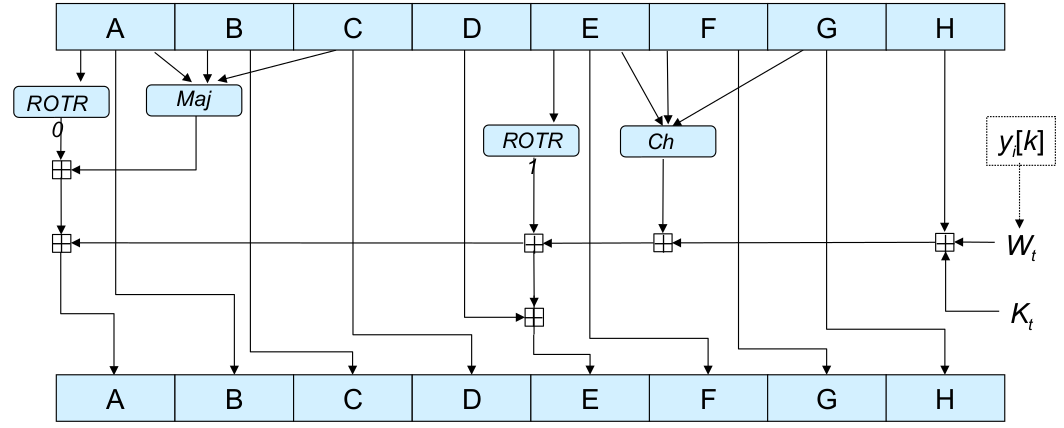
\includegraphics[width=.5\linewidth]{Assets/NetworkSecurity-sha-2.png}
                        \item $t\in{0, ..., 15}\Rightarrow W_t:=y_i,,t''$
                        \item $t\in{16, ..., r}\Rightarrow W_t:=W_{t-16}\oplus \delta_0(W_{t-15})\oplus W_{t-7}\oplus\delta_1(W_{t-2})$
                        \item $K_t$ ist der gebrochene Teil der Kubikwurzel aus der t-ten Primzahl
                        \item Die ROTR- und Funktionen XOR-verknüpfen verschiedene Verschiebungen des Eingangswertes
                        \item $Ch$ und $Maj$ sind logische Kombinationen der Eingabewerte
                  \end{itemize*}
                  \item Alles in allem sehr ähnlich zu SHA-1
                  \item Aufgrund der Größe und komplizierteren Rundungsfunktionen etwa 30-50\% langsamer als SHA-1
                  \item Sicherheitsdiskussion
                  \begin{itemize*}
                        \item Bereits 2004 wurde entdeckt, dass eine vereinfachte Version des Algorithmus (mit XOR statt Addition und symmetrischen Konstanten) hochkorrelierte Ausgaben erzeugt
                        \item Für rundenreduzierte Versionen von SHA-2 gibt es Pre-Image-Angriffe, die schneller sind als Brute-Force, aber sehr unpraktisch
                        \item Auch wenn Größe und Komplexität derzeit keine Angriffe zulassen, ist die Situation unangenehm
                        \item Dies führte zur Notwendigkeit eines neuen SHA-3-Standards
                  \end{itemize*}
            \end{itemize*}
      \end{itemize*}

      \subsection{Der sichere Hash-Algorithmus SHA-3}
      \begin{itemize*}
            \item Sicherheitsbedenken bezüglich SHA-1 und SHA-2
            \begin{itemize*}
                  \item Oktober 2012: Keccak wird zu SHA-3
                  \item SHA-3 ist sehr schnell, besonders in der Hardware
                  \item Sehr gut dokumentiert und analysierbar
            \end{itemize*}
            \item Keccak basiert auf einer so genannten Schwammkonstruktion anstelle der früheren Merkle-Dåmgard-Konstruktionen
            \item Vielseitiges Design, um fast alle symmetrischen kryptographischen Funktionen zu implementieren
            \item Arbeitet normalerweise in 2 Phasen
            \begin{description*}
                  \item[Absorbieren] von Informationen beliebiger Länge in $1600$Bit des internen Zustands
                  \item[Auspressen] (d.h. Ausgeben) von Hash-Daten beliebiger Länge (nur 224, 256, 384 und 512 Bit standardisiert)
            \end{description*}
            \item Der interne Zustand ist in 2 Registern organisiert
            \begin{itemize*}
                  \item Ein Register der Größe $r$ ist ,,public'': Eingabedaten werden in der Absorptionsphase mit XOR verknüpft, Ausgabedaten werden in der Quetschungsphase daraus abgeleitet
                  \item Das Register der Größe $c$ ist ,,privat'': Ein- und Ausgabe wirken sich nicht direkt auf es aus
                  \item In Keccak ist die Größe der Register ($c+r=$)$1600$Bits
                  \item Die Größe von $c$ ist doppelt so groß wie die Länge des Ausgangsblocks
                  \item Beide Register werden mit $0$ initialisiert
            \end{itemize*}
            \item Das Hashing erfolgt durch eine Funktion $f$, die die Register liest und einen neuen Zustand ausgibt
            \item Sponge-Konstruktion
            \begin{itemize*}
                  \item 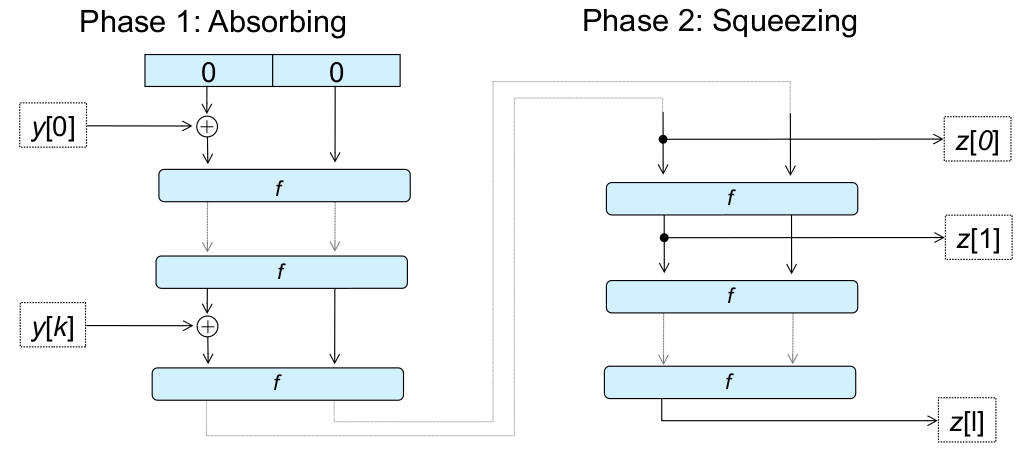
\includegraphics[width=.6\linewidth]{Assets/NetworkSecurity-sha-3.png}
                  \item Absorption: $k+1$ Eingabeblöcke der Größe $r$ werden in den Zustand gemischt
                  \item Quetsch: $l+1$ Ausgangsblöcke der Größe $r$ werden erzeugt (oft nur einer)
                  \item letzter Eingabe- und Ausgabeblock auffüllen oder abschneiden
            \end{itemize*}
            \item Die Funktion f
            \begin{itemize*}
                  \item Offensichtlich hängt die Sicherheit einer Sponge-Konstruktion von der Sicherheit von f
                  \item Keccak verwendet 24 Runden von 5 verschiedenen Unterfunktionen $(\Sigma,\rho,\pi,\chi,\iota)$, um f zu implementieren
                  \item Die Unterfunktionen operieren auf einem ,,dreidimensionalen'' Bit-Array a $[5][5][w]$, wobei $w$ entsprechend der Größe $r$ und $c$ gewählt wird
                  \item Alle Operationen werden über $GF(2^n)$ durchgeführt
                  \item Jede der Unterfunktionen gewährleistet bestimmte Eigenschaften
                  \begin{itemize*}
                        \item Schnelle Diffusion der geänderten Bits im gesamten Zustand ($\Sigma$)
                        \item Langfristige Diffusion ($\pi$)
                        \item Sicherstellung, dass f nichtlinear wird ($\chi$)
                        \item Rundenspezifische Substitution ($\iota$)
                  \end{itemize*}
            \end{itemize*}
            \item $\Sigma$ wird zuerst ausgeführt, um sicherzustellen, dass sich der geheime und der öffentliche Zustand schnell vermischen, bevor andere Unterfunktionen angewendet werden
            \item Sicherheit
            \begin{itemize*}
                  \item Derzeit gibt es keine nennenswerten Schwachstellen in SHA-3
                  \item Die bekanntesten Pre-Image-Angriffe funktionieren nur mit einer Funktion f mit bis zu 8 Runden
                  \item Zum Schutz vor internen Kollisionen sollten 11 Runden ausreichen
                  \item Im Vergleich zu SHA-1 und SHA-2 werden zusätzliche Sicherheitseigenschaften garantiert, da der interne Zustand nie öffentlich gemacht wird
                  \item Verhindert Angriffe, bei denen beliebige Informationen zu einer gültigen geheimen Nachricht hinzugefügt werden
                  \item Bietet Chosen Target Forced Prefix (CTFP) Preimage-Resistenz, d.h. es ist nicht möglich, eine Nachricht $m=P||S$ zu konstruieren, wobei $P$ fest und $S$ beliebig gewählt ist, s.t. $H(m)=y$
                  \item Für Merkle-Dåmgard-Konstruktionen ist dies nur so schwer wie die Kollisionssicherheit
                  \item Keine schnelle Möglichkeit, Multikollisionen schnell zu erzeugen
            \end{itemize*}
      \end{itemize*}

      \subsection{Cipher Block Chaining MAC}
      \begin{itemize*}
            \item CBC-MAC wird berechnet, indem Nachricht im CBC-Modus verschlüsselt und letzte Chiffretextblock oder Teil davon als MAC verwendet wird
            \item 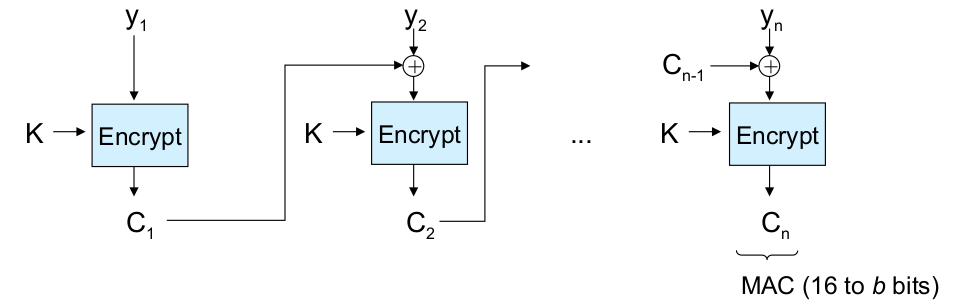
\includegraphics[width=.5\linewidth]{Assets/NetworkSecurity-CBC-mac.png}
            \item MAC muss nicht mehr signiert werden, da bereits mit gemeinsamen Geheimnis K erzeugt
            \item Es ist jedoch nicht möglich zu sagen, wer genau einen MAC erstellt hat, da jeder (Sender, Empfänger), der den geheimen Schlüssel K kennt, dies tun kann
            \item Verfahren funktioniert mit jeder Blockchiffre (DES, IDEA, ...)
            \item Sicherheit von CBC-MAC
            \begin{itemize*}
                  \item Da Angreifer K nicht kennt, ist Geburtstagsangriff sehr viel schwieriger
                  \item Ein Angriff auf einen CBC-MAC erfordert bekannte Paare (Nachricht, MAC)
                  \item ermöglicht kürzere MACs
                  \item Ein CBC-MAC kann optional verstärkt werden, indem man sich auf einen zweiten Schlüssel $K'\not= K$ einigt und eine dreifache Verschlüsselung des letzten Blocks durchführt: $MAC:=E(K,D(K',E(K,C_{n-1})))$
                  \item Dadurch verdoppelt sich der Schlüsselraum bei nur geringem Rechenaufwand
                  \item Die Konstruktion ist nicht sicher, wenn die Nachrichtenlängen variieren
            \end{itemize*}
            \item Es gibt auch einige Vorschläge, MDCs aus symmetrischen Blockchiffren zu erzeugen, indem der Schlüssel auf einen festen (bekannten) Wert gesetzt wird
            \begin{itemize*}
                  \item Wegen der relativ kleinen Blockgröße von 64 Bit der meisten gängigen Blockchiffren bieten diese Verfahren keine ausreichende Sicherheit gegen Geburtstagsangriffe
                  \item Da symmetrische Blockchiffren mehr Rechenaufwand erfordern als spezielle kryptografische Hash-Funktionen, sind diese Verfahren relativ langsam
            \end{itemize*}
      \end{itemize*}

      \subsection{Konstruktion eines MAC aus einem MDC}
      \begin{itemize*}
            \item Grund für die Konstruktion von MACs aus MDCs Kryptografische Hash-Funktionen laufen im Allgemeinen schneller ab als symmetrische Blockchiffren
            \item Grundidee: ,,mix'' einen geheimen Schlüssel K mit der Eingabe und berechne einen MDC
            \item Die Annahme, dass ein Angreifer K kennen muss, um einen gültigen MAC zu erzeugen, wirft dennoch einige kryptografische Probleme auf (zumindest für Merkle-Dåmgard-Hash-Funktionen)
            \begin{itemize*}
                  \item Die Konstruktion $H(K||m)$ ist nicht sicher
                  \item Die Konstruktion $H(m||K)$ ist nicht sicher
                  \item Die Konstruktion $H(K||p||m||K)$, bei der p ein zusätzliches Auffüllfeld bezeichnet, bietet keine ausreichende Sicherheit
            \end{itemize*}
            \item häufigste verwendete Konstruktion ist $H(K\oplus p_1||H(K\oplus p_2||m))$
            \begin{itemize*}
                  \item Schlüssel wird mit $0$ aufgefüllt, um den Schlüssel zu einem Eingabeblock der kryptographischen Hashfunktion aufzufüllen
                  \item Zwei verschiedene konstante Muster $p_1$ und $p_2$ werden mit dem aufgefüllten Schlüssel XOR-verknüpft
                  \item Dieses Schema scheint sicher zu sein
                  \item Es wurde in RFC 2104 standardisiert und wird HMAC genannt
            \end{itemize*}
      \end{itemize*}

      \subsection{Authentifizierte Verschlüsselung mit zugehörigen Daten (AEAD) Modi}
      \begin{itemize*}
            \item Normalerweise sind die Daten nicht authentifiziert oder verschlüsselt, sondern verschlüsselt UND authentifiziert %(Blöcke $P_0...P_n$)
            \item Manchmal müssen zusätzliche Daten authentifiziert werden (z.B. Paketköpfe), im Folgenden mit $A_0...A_m$ bezeichnet
            \item führte zur Entwicklung von AEAD-Betriebsarten
            \item Beispiele hierfür sind
            \begin{itemize*}
                  \item Galois/Zähler-Modus (GCM)
                  \item Zähler mit CBC-MAC (CCM)
                  \item Offset-Codebuch-Modus (OCM)
                  \item SpongeWrap
            \end{itemize*}
      \end{itemize*}

      \subsubsection{Galois/Zähler-Modus (GCM)}
      \begin{itemize*}
            \item Beliebter AEAD-Modus
            \item NIST-Standard, Teil von IEEE 802.1AE, IPsec, TLS, SSH usw.
            \item Frei von Patenten
            \item wegen seiner hohen Geschwindigkeit hauptsächlich in Netzwerkanwendungen eingesetzt
            \begin{itemize*}
                  \item Äußerst effizient in der Hardware
                  \item Prozessorunterstützung auf neueren x86-CPUs
                  \item Zeitintensive Aufgaben können vorberechnet und parallelisiert werden
                  \item Keine Notwendigkeit für Auffüllungen
            \end{itemize*}
            \item Verwendet konventionelle Blockchiffre mit 128-Bit-Blockgröße (z.B. AES)
            \item Berechnet MAC durch Multiplikationen und Additionen in $GF(2^{128})$ über das irreduzible Polynom $x^{128}+x^{7}+x^{2}+x+1$
            \item Erfordert nur $n+1$ Blockchiffre-Aufrufe pro Paket (n = Länge der verschlüsselten und authentifizierten Daten)
            %\item 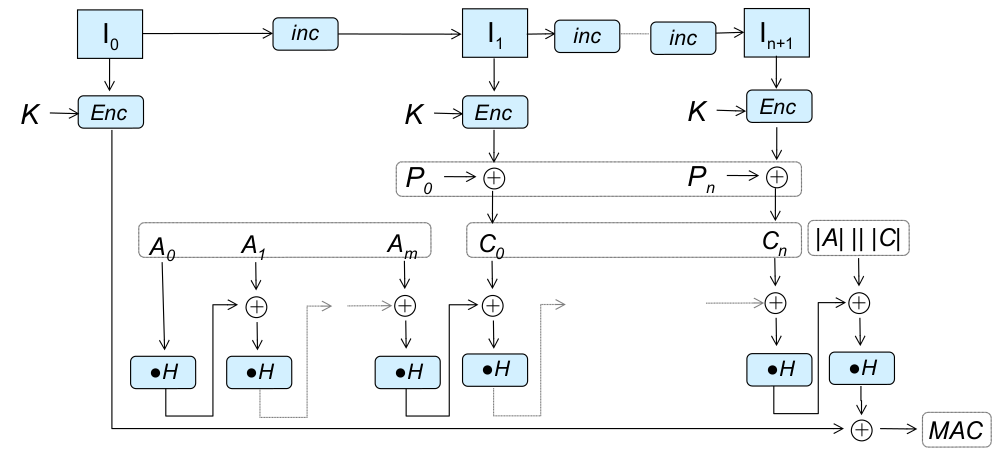
\includegraphics[width=\linewidth]{Assets/NetworkSecurity-gcm.png}
            \begin{itemize*}
                  \item $I_0$ wird mit dem IV und einem Padding oder einem Hash des IV initialisiert (wenn er nicht 96 Bit beträgt)
                  \item $\circ H$ ist $GF(2^{128})$ Multiplikation mit $H=E(K,0^{128})$
                  \item Eingabeblöcke $A_m$ und $P_n$ auf 128 Bit aufgefüllt
                  \item $A_m$ und $C_n$ vor Ausgabe auf die Originalgröße gekürzt
                  \item letzte Authentifizierung verwendet 64 Bit kodierte Bitlängen von $A$ und $C$
            \end{itemize*}
            \item Sicherheit
            \begin{itemize*}
                  \item Schneller Modus, erfordert aber einige Sorgfalt
                  \item Erwiesenermaßen sicher %(unter bestimmten Voraussetzungen, z.B. wenn die verwendete Blockchiffre nicht von Zufallszahlen unterscheidbar ist)
                  aber die Konstruktion ist anfällig
                  \item IVs dürfen NICHT wiederverwendet werden, da sonst Datenströme XOR-verknüpft werden können und das XOR der Datenströme wiederhergestellt werden kann, was zu einer sofortigen Wiederherstellung des geheimen Werts $H$ führen kann
                  \item H hat einen möglichen schwachen Wert $0^{128}$, in diesem Fall wird die Authentifizierung nicht funktionieren, und wenn IVs mit einer anderen Länge als 96 Bits verwendet werden, wird $C_0$ immer gleich sein
                  \item Einige andere Schlüssel erzeugen Hash-Schlüssel mit einer niedrigen Ordnung, was vermieden werden muss...
                  \item Erfolgreiche Fälschungsversuche können Informationen über H durchsickern lassen, daher MÜSSEN kurze MAC-Längen vermieden oder risikominimiert werden
                  \item Die erreichte Sicherheit ist nur $2^{t-k}$ und nicht $2^t$ (für MAC-Länge t und Anzahl der Blöcke $2^k$), da Blöcke modifiziert werden können, um nur Teile des MAC zu ändern
            \end{itemize*}
      \end{itemize*}

      \subsubsection{Exkurs: Rechenoperationen in $GF(2^n)$}
      \begin{itemize*}
            \item Galoisfeld-Arithmetik definiert über Termen (z.B. $a_3x^3+a_2x^2+a_1x+a_0$)
            \item Koeffizienten sind Elemente des Feldes $\mathbb{Z}_2$, d.h. entweder 0 oder 1
            \item Oft werden nur die Koeffizienten gespeichert, so wird aus $x^4+x^2 +x^1=$ 0x16
            \item Die Addition in $GF(2^n)$ ist einfach die Addition von Termen
            \begin{itemize*}
                  \item Da gleiche Koeffizienten auf 0 abbilden, XOR der Werte
                  \item Extrem schnell in Hard- und Software
            \end{itemize*}
            \item Multiplikation in $GF(2^n)$ ist Polynommultiplikation und Modulodivision durch irreduzibles Polynom vom Grad $n$
            \begin{itemize*}
                  \item Irreduzible Polynome sind nicht ohne Rest durch irgendein anderes Polynom teilbar, außer durch $1$, ähnlich wie Primzahlen in GF
                  \item Kann durch eine Reihe von Verschiebe- und XOR-Operationen implementiert werden
                  \item Sehr schnell in Hardware oder auf neueren Intel-CPUs
                  \item Modulo-Operation kann wie bei einer regulären CRC-Berechnung durchgeführt werden
            \end{itemize*}
            %\item Addition Beispiel: $x^3 +x+1 x\oplus x^2+x = x^3 +x^2 +1 \leftrightarrow$ 0x0B XOR 0x06 = 0x0D
            %\item Multiplikationsbeispiel (über $x^4 +x+1$): $x^3 +x+1\circ x^2+x = x^5+x^3+x^2\oplus x^4+x^2+x\ mod\ x^4+x+1=x^5+x^4+x^3+x\ mod\ x^4+x+1 = x^3 +x^2 +x+1$
            \item Elemente von $GF(2^n)$ (mit Ausnahme von 1 und dem irreduziblen Polynom) können ein Generator für die Gruppe sein
            %\item Beispiel für x und das Polynom $x^4+x+1:x,x^2,x^3,x+1,x^2+x,x^3+x^2,x^3+x+1,x^2 +1,x^3+x,x^2+x+1,x^3+x^2+x,x^3+x^2+x+1,x^3+x^2+1,x^3+1,1,x,...$
            \item Andere Konzepte endlicher Gruppen gelten ebenfalls, z.B. hat jedes Element ein multiplikatives inverses Element
            \item Kann durch eine angepasste Version des Erweiterten Euklidischen Algorithmus gefunden werden
      \end{itemize*}

      \subsection{SpongeWrap}
      \begin{itemize*}
            \item mit SHA-3 möglich, ein AEAD-Konstrukt zu implementieren
            \item Konstruktion sehr einfach und leicht zu verstehen
            \item Verwendet Duplex-Modus für Sponge-Funktionen, bei dem Schreib- und Leseoperationen verschachtelt werden
            \item Erfordert kein Auffüllen der Daten auf eine bestimmte Blockgröße
            \item Kann nicht parallelisiert werden
            \item Sicherheit
            \begin{itemize*}
                  \item nicht weit verbreitet, Aspekte genauso sicher wie SHA-3 im standardisierten Modus
                  \item Wenn die authentifizierten Daten A keine eindeutige IV enthalten, wird derselbe Schlüsselstrom erzeugt %(ermöglicht die Wiederherstellung eines Blocks XOR-verschlüsselter Daten)
                  %\item 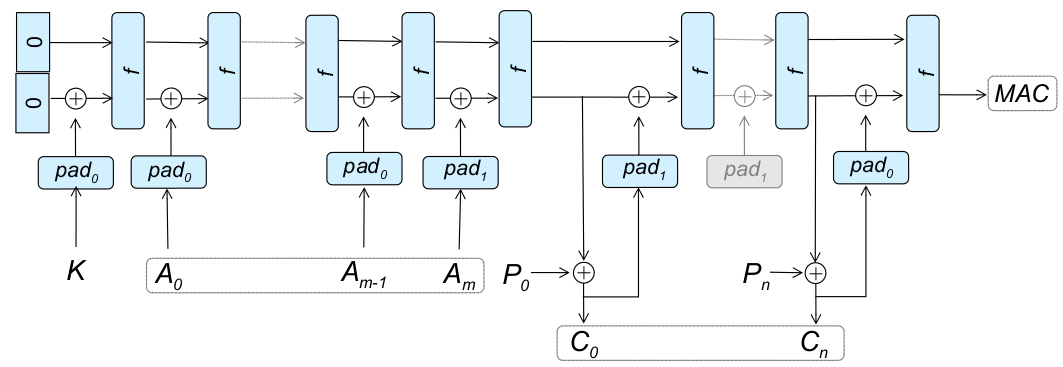
\includegraphics[width=\linewidth]{Assets/NetworkSecurity-sponge-wrap.png}
                  \item Vereinfachte Version, bei der die Länge von Schlüssel und MAC kleiner sein muss als die Blockgröße
                  \item Auffüllungen mit einem einzelnen $0$- oder $1$-Bit stellen sicher, dass verschiedene Datenblocktypen gut voneinander getrennt sind
            \end{itemize*}
      \end{itemize*}

      \section{Zufallszahlengenerierung}
      \subsection{Aufgaben der Schlüsselverwaltung}
      \begin{description*}
            \item[Erzeugung] Für die Sicherheit ist es von entscheidender Bedeutung, dass die Schlüssel mit einem wirklich zufälligen oder zumindest pseudozufälligen Generierungsverfahren erzeugt werden
            %\item Andernfalls könnte ein Angreifer den Schlüsselgenerierungsprozess reproduzieren und den zur Sicherung einer bestimmten Kommunikation verwendeten Schlüssel leicht finden
            \item[Verteilung]
            \begin{itemize*}
                  \item einiger anfänglicher Schlüssel in der Regel manuell / ,,out of band,, erfolgen
                  \item Sitzungsschlüssel verteilung in der Regel während eines Authentifizierungsaustauschs durchgeführt
                  %\item Beispiele: Diffie-Hellman, Otway-Rees, Kerberos, X
            \end{itemize*}
            \item[Speicherung]
            \begin{itemize*}
                  \item Schlüssel sollten sicher gespeichert werden
                  \item verschlüsselt mit einer schwer zu erratenden Passphrase oder
                  \item in einem sicheren Gerät wie einer Smart-Card
            \end{itemize*}
            \item[Entzug] Wenn ein Schlüssel kompromittiert wurde, sollte es möglich sein, diesen Schlüssel zu widerrufen, damit er nicht mehr missbraucht werden kann (vgl. X.509)
            \item[Vernichtung] Schlüssel, die nicht mehr verwendet werden, sollten sicher vernichtet werden
            \item[Wiederherstellung]
            \begin{itemize*}
                  \item Wenn ein Schlüssel verloren gegangen ist, sollte er wiederhergestellt werden können, um Datenverluste zu vermeiden
                  \item Die Wiederherstellung von Schlüsseln ist nicht zu verwechseln mit der Schlüsselhinterlegung
            \end{itemize*}
            \item[Hinterlegung] Mechanismen und Architekturen, die es staatlichen Stellen ermöglichen sollen, Sitzungsschlüssel zu erhalten, um zu Strafverfolgungszwecken die Kommunikation abzuhören/gespeicherte Daten zu lesen
            %\item Wenn ich meinen Schlüssel zurückbekomme, ist es Schlüsselwiederherstellung, wenn du meinen Schlüssel zurückbekommst, ist es Schlüsselhinterlegung...
      \end{description*}

      \subsection{Zufalls- und Pseudo-Zufallszahlengenerierung}
      \begin{itemize*}
            \item Ein \textbf{Zufallsbitgenerator} ist ein Gerät oder ein Algorithmus, der eine Folge statistisch unabhängiger und unverfälschter Binärziffern ausgibt
            \item Ein Zufallsbitgenerator kann zur Erzeugung gleichmäßig verteilter Zufallszahlen verwendet werden, z.B. kann eine zufällige ganze Zahl im Intervall $[0,n]$ erhalten werden, indem eine zufällige Bitfolge der Länge $\lfloor lg\ n\rfloor+1$ erzeugt und in eine Zahl umgewandelt wird %Ist die resultierende ganze Zahl größer als n, so kann sie verworfen werden, und der Vorgang wird so lange wiederholt, bis eine ganze Zahl im gewünschten Bereich erzeugt worden ist
            \item Ein \textbf{Pseudo-Zufallsbitgenerator} (PRBG) ist ein deterministischer Algorithmus, der bei einer wirklich zufälligen Binärfolge der Länge $k$ eine Binärfolge der Länge $m>>k$ ausgibt, die zufällig erscheint. Die Eingabe in den PRBG wird als Seed bezeichnet, die Ausgabe als pseudozufällige Bitfolge
            \item Die Ausgabe eines PRBG ist nicht zufällig, tatsächlich ist die Anzahl der möglichen Ausgabesequenzen der Länge $m$ höchstens ein kleiner Bruchteil $2^k/2^m$, da der PRBG immer dieselbe Ausgabesequenz für einen (festen) Seed erzeugt
            \item Die Motivation für die Verwendung einer PRBG ist, dass es zu teuer sein könnte, echte Zufallszahlen der Länge $m$ zu erzeugen, so dass nur eine kleinere Menge von Zufallsbits erzeugt wird und dann aus den $k$ echten Zufallsbits eine pseudozufällige Bitfolge erzeugt wird
            \item Um Vertrauen in die Zufälligkeit einer Pseudo-Zufallsfolge zu gewinnen, werden statistische Tests mit den erzeugten Folgen durchgeführt
            %\item Beispiel
            %\begin{itemize*}
            %      \item Ein linearer Kongruenzgenerator erzeugt eine Pseudo-Zufallsfolge von Zahlen $y_1,y_2, ...$ gemäß der linearen Rekursion $y_i= a\times y_{i-1} + b\ mod\ q$, wobei $a, b, q$ Parameter sind, die den PRBG charakterisieren
            %      \item Leider ist dieser Generator auch dann vorhersehbar, wenn $a, b$ und $q$ unbekannt sind, und sollte daher nicht für kryptographische Zwecke verwendet werden
            %\end{itemize*}
            \item Sicherheitsanforderungen an PRBGs
            \begin{itemize*}
                  \item Als Mindestsicherheitsanforderung sollte die Länge $k$ des Seeds einer PRBG so groß sein, dass eine Brute-Force-Suche über alle Seeds für einen Angreifer nicht durchführbar ist
                  \item Die Ausgabe einer PRBG sollte statistisch nicht von echten Zufallssequenzen unterscheidbar sein
                  \item Die Ausgabebits sollten für einen Angreifer mit begrenzten Ressourcen unvorhersehbar sein, wenn er den Seed nicht kennt
            \end{itemize*}
            \item Ein PRBG besteht alle statistischen Polynomialzeit-Tests, wenn kein deterministischer polynomialzeit-Algorithmus zwischen einer Ausgangssequenz des Generators und einer echten Zufallssequenz derselben Länge mit einer Wahrscheinlichkeit deutlich größer als $0$ unterscheiden kann
            \item Polynomialzeit-Algorithmus bedeutet, dass die Laufzeit des Algorithmus durch ein Polynom in der Länge $m$ der Sequenz begrenzt ist
            \item Ein PRBG besteht den Next-Bit-Test, wenn es keinen deterministischen Polynomialzeit-Algorithmus gibt, der bei Eingabe der ersten $m$ Bits einer Ausgangssequenz $s$ das $(m+1)$-te Bit $s_{m+1}$ der Ausgangssequenz mit einer Wahrscheinlichkeit deutlich größer als $0$ vorhersagen kann
            \item Theorem: Wenn eine PRBG den Next-Bit-Test $\Leftrightarrow$ besteht, dann besteht sie alle statistischen Polynomialzeittests
            \item Ein PRBG, der den Next-Bit-Test besteht wird als kryptographisch sicherer Pseudo-Zufallsgenerator (CSPRBG) bezeichnet
      \end{itemize*}

      \subsection{Zufallszahlengenerierung}
      \begin{itemize*}
            \item Hardware-basierte Zufallsbit-Generatoren basieren auf physikalischen Phänomenen, wie
            \begin{itemize*}
                  \item Zeit zwischen Emission von Teilchen bei radioaktiven Zerfall
                  \item thermisches Rauschen einer Halbleiterdiode,
                  \item Frequenzinstabilität eines Oszillators,
                  %\item der Betrag, um den ein Metall-Isolator-Halbleiter-Kondensator während eines bestimmten Zeitraums aufgeladen wird,
                  %\item Luftturbulenzen in einem versiegelten Festplattenlaufwerk, die zufällige Schwankungen in den Sektor-Lese-Latenzen des Festplattenlaufwerks verursachen, und
                  \item Ton von Mikrofon oder Video einer Kamera
                  %\item der Zustand einer ungeraden Anzahl von kreisförmig verbundenen NOT-Gattern
            \end{itemize*}
            \item hardwarebasierte Zufallsbitgenerator sollte idealerweise in einer manipulationssicheren Vorrichtung untergebracht und so vor möglichen Angreifern geschützt sein
            \item Softwarebasierte Zufallsbit-Generatoren können auf Prozessen basieren wie
            \begin{itemize*}
                  \item der Systemuhr,
                  \item der verstrichenen Zeit zwischen Mausbewegungen,
                  \item Inhalt von Eingabe-/Ausgabepuffern
                  %\item Benutzereingaben und
                  \item Werte des Betriebssystems wie Systemauslastung %und Netzwerkstatistiken
            \end{itemize*}
            \item Idealerweise sollten mehrere Zufallsquellen ,,gemischt'' werden um zu verhindern, dass ein Angreifer den Zufallswert erraten kann
            %\item Wird z.B. nur die Systemuhr als Zufallsquelle verwendet, könnte ein Angreifer die aus dieser Zufallsquelle gewonnenen Zufallszahlen erraten, wenn er weiß, wann sie erzeugt wurden.
            \item Verzerrung: Betrachte einen Zufallsgenerator, der verzerrte, aber unkorrelierte Bits erzeugt, z.B. $1$en mit $p\not= 0,5$ und $0$en mit $1-p$, wobei $p$ unbekannt aber fest ist
            \item folgende Technik kann verwendet werden, um eine Zufallsfolge zu erhalten, die unkorreliert und unverzerrt ist
            \begin{itemize*}
                  \item Ausgangssequenz des Generators in Bitpaare gruppiert
                  \item Alle Paare $00$ und $11$ werden verworfen
                  \item Für jedes Paar $10$ erzeugt der unvoreingenommene Generator eine $1$ und für jedes Paar $01$ eine $0$
            \end{itemize*}
            \item Ein weiteres praktisches Verfahren zur Entzerrung ist Weiterleitung von Sequenzen, deren Bits korreliert oder verzerrt sind, durch eine kryptografische Hash-Funktion wie MD5 oder SHA-1
      \end{itemize*}

      \subsection{Statistische Tests für Zufallszahlen}
      Mit den folgenden Tests lässt sich überprüfen, ob eine generierte Zufalls- oder Pseudozufallsfolge bestimmte statistische Eigenschaften nicht erfüllt
      \begin{description*}
            \item[Monobit-Test] Gibt es gleich viele 1en wie 0en?
            \item[Serieller Test] Gibt es gleich viele 00-, 01-, 10-, 11-Paare?
            \item[Poker-Test] Gibt es gleich viele Sequenzen $ni$ der Länge $q$, die mit $q$ den gleichen Wert haben, so dass $\lfloor m/q\rfloor\geq 5\times (2^q)$
            \item[Test auf Durchläufe] Entspricht die Anzahl der Läufe unterschiedlicher Länge den Erwartungen für Zufallszahlen?
            \item[Autokorrelationstest] Gibt es Korrelationen zwischen der Sequenz und verschobenen Versionen davon?
            \item[Maurer's Universal Test] Kann die Sequenz komprimiert werden?
            \item[NIST SP 800-22] Standardisierte Testsuite, umfasst die oben genannten und weitere fortgeschrittene Tests
      \end{description*}

      \subsection{Sichere Pseudo-Zufallszahlengenerierung}
      \begin{itemize*}
            \item Es gibt eine Reihe von Algorithmen, die kryptografische Hash-Funktionen oder Verschlüsselungsalgorithmen zur Erzeugung von kryptografisch sicheren Pseudozufallszahlen verwenden
            \item Obwohl diese Verfahren nicht als sicher bewiesen werden können, scheinen sie für die meisten praktischen Situationen ausreichend
            \item Ein solcher Ansatz ist der Generator ANSI X9.17
            \begin{itemize*}
                  \item Eingabe: ein zufälliger und geheimer 64-Bit-Seed s, eine ganze Zahl m und ein 3-DES-Schlüssel K
                  \item Ausgabe: m pseudo-zufällige 64-Bit-Strings $y_1,y_2,...Y_m$
                  \begin{enumerate*}
                        \item $q = E(K, Date_Time)$
                        \item for $i$ von $1$ bis $m$ do
                        \begin{enumerate*}
                              \item $x_i = E(K, (q\oplus s)$
                              \item $s = E(K, (x_i\oplus q)$
                        \end{enumerate*}
                        \item $Return(x_1,x_2,...x_m)$
                  \end{enumerate*}
                  %\item Diese Methode ist eine vom U.S. Federal Information Processing Standard (FIPS) zugelassene Methode zur pseudozufälligen Erzeugung von Schlüsseln und Initialisierungsvektoren zur Verwendung mit DES
            \end{itemize*}
            \item Das RSA-PRBG ist ein CSPRBG unter der Annahme, dass das RSA-Problem unlösbar ist
            \begin{itemize*}
                  \item Ausgabe: eine pseudo-zufällige Bitfolge $z_1,z_2,...,z_k$ der Länge $k$
            \end{itemize*}
            \begin{enumerate*}
                  \item Setup-Prozedur: Erzeuge zwei geheime Primzahlen $p, q$, die für die Verwendung mit RSA geeignet sind. Berechne $n=p\times q$ und $\phi=(p-1)\times(q-1)$. Wähle eine zufällige ganze Zahl $e$ so, dass $1< e<\phi$ und $gcd(e,\phi)=1$
                  \item Wähle eine zufällige ganze Zahl $y_0$ (Seed) so, dass $y_0\in ,,1,n''$
                  \item Für $i$ von $1$ bis $k$ tun
                  \begin{enumerate*}
                        \item $y_i=(y_{i-1})^e\ mod\ n$
                        \item $z_i =$ das niedrigstwertige Bit von $y_i$
                  \end{enumerate*}
            \end{enumerate*}
            \begin{itemize*}
                  \item Die Effizienz des Generators kann leicht verbessert werden, indem man die letzten $j$ Bits von jedem $y_i$ nimmt, wobei $j=c\times lg(lg(n))$ und $c$ eine Konstante ist
                  \item Für eine gegebene Bitlänge $m$ von $n$ wurde jedoch noch kein Wertebereich für die Konstante $c$ ermittelt, in dem der Algorithmus noch einen CSPRBG ergibt
            \end{itemize*}
            \item Der Blum-Blum-Shub-PRBG ist ein CSPRBG unter der Annahme, dass das Problem der ganzzahligen Faktorisierung unlösbar ist
            \begin{itemize*}
                  \item Ausgabe: eine pseudo-zufällige Bitfolge $z_1,z_2,...,z_k$ der Länge $k$
            \end{itemize*}
            \begin{enumerate*}
                  \item Setup-Prozedur: Erzeuge zwei große geheime und unterschiedliche Primzahlen $p,q$, so dass $p,q$ jeweils kongruent 3 modulo 4 sind, und lass $n=p\times q$
                  \item Wähle eine zufällige ganze Zahl $s$ (Seed) so, dass $s\in ,,1, n-1''$ liegt, so dass $gcd(s,n)=1$ und $y_0=s^2\ mod\ n$
                  \item Für $i$ von $1$ bis $k$ tun
                  \begin{enumerate*}
                        \item $y_i = (y_{i-1})^2\ mod\ n$
                        \item $z_i =$ das niedrigstwertige Bit von $y_i$
                  \end{enumerate*}
            \end{enumerate*}
            \begin{itemize*}
                  \item Die Effizienz des Generators kann mit der gleichen Methode wie beim RSA-Generator verbessert werden, wobei ähnliche Einschränkungen für die Konstante c gelten
            \end{itemize*}
            \item Dualer deterministischer Zufallsbitgenerator mit elliptischer Kurve
            \begin{itemize*}
                  \item Basierend auf der Unlösbarkeit des Problems des diskreten Logarithmus elliptischer Kurven
                  \item Vereinfachte Version: 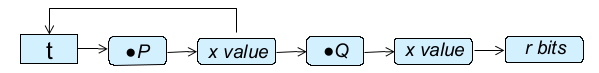
\includegraphics[width=.6\linewidth]{Assets/NetworkSecurity-dual-elliptic-curve-deterministic-random-bit-generator.png}
                  \item Der Zustand $t$ wird mit einem Generator $P$ multipliziert, der x-Wert des neuen Punktes wird zu $t'$
                  \item Multiplikation mit einem anderen Punkt $Qr$ Bits der Ausgabe können erzeugt werden, die Anzahl der Bits hängt von der Kurve ab %(zwischen 240 und 504 Bits)
                  \item Teil der Norm NIST 800-90A
                  \item Sicherheit:  Es wurde gezeigt, dass Angreifer den Zustand $t$ ableiten können, wenn $P$ für eine Konstante $e$ gleich $eQ$ gewählt wird.
                  \item Wir wissen nicht, wie die vordefinierten Punkte $P$ und $Q$ in NIST 800-90A abgeleitet werden, also Vorsicht
            \end{itemize*}
      \end{itemize*}

      \subsection{CSPRNG-Sicherheit ist eine große Sache!}
      \begin{itemize*}
            \item Im September 2006 wurde Debian versehentlich so verändert, dass nur die Prozess-ID verwendet wurde, um den OpenSSL CSPRNG zu füttern. Nur 32.768 mögliche Werte
            \item Ein Scan von etwa 23 Millionen TLS- und SSH-Hosts zeigte, dass
            \begin{itemize*}
                  \item Mindestens 0,34\% der Hosts teilten Schlüssel% aufgrund fehlerhafter RNGs
                  \item 0,50\% der gescannten TLS-Schlüssel aufgrund einer geringen Zufälligkeit kompromittiert werden konnten
                  \item und 1,06\% der SSH-Hosts
            \end{itemize*}
            \item Überwache den verwendeten CSPRNG
            \item Generiere keine Zufallszahlen direkt nach dem Booten% des Systems
            \item Verwende blockierende RNGs, d.h. solche, die nicht fortfahren, bis sie genügend Entropie haben
      \end{itemize*}

      \pagebreak
      \section{Kryptographische Protokolle}
      \begin{itemize*}
            \item Ein kryptographisches Protokoll ist definiert als eine Reihe von Schritten und der Austausch von Nachrichten zwischen mehreren Einheiten, um ein bestimmtes Sicherheitsziel zu erreichen
            \item Eigenschaften eines Protokolls
            \begin{itemize*}
                  \item Jeder, der an dem Protokoll beteiligt ist, muss das Protokoll und alle zu befolgenden Schritte im Voraus kennen
                  \item Jeder, der an dem Protokoll beteiligt ist, muss zustimmen, es zu befolgen
                  \item Das Protokoll muss eindeutig sein, d.h. jeder Schritt ist genau definiert und es gibt keine Möglichkeit für Missverständnisse
                  \item Das Protokoll muss vollständig sein, d.h. es gibt für jede mögliche Situation eine bestimmte Aktion
            \end{itemize*}
            \item Zusätzliche Eigenschaft eines kryptographischen Protokolls
            \begin{itemize*}
                  \item Es sollte nicht möglich sein, mehr zu tun oder zu erfahren als das, was im Protokoll angegeben ist
            \end{itemize*}
      \end{itemize*}

      \subsection{Anwendungen von kryptographischen Protokollen}
      \begin{itemize*}
            \item Schlüsselaustausch
            \item Authentifizierung der Datenherkunft/Entitäten
            \item Kombinierte Authentifizierung und Schlüsselaustausch
            \item Aufteilung des Geheimnisses (alle Teile werden für Rekonstruktion benötigt)
            \item Gemeinsame Nutzung des Geheimnisses (m von n Teilen werden für Rekonstruktion benötigt)
            \item Zeitstempelung
            \item Schlüsselhinterlegung (Sicherstellung, dass nur eine befugte Stelle Schlüssel wiederherstellen kann)
            \item Zero-Knowledge-Beweise (Nachweis der Kenntnis einer Information ohne Offenlegung der Information)
            \item Blindsignaturen (nützlich für die Wahrung der Privatsphäre bei Zeitstempeldiensten)
            \item Sichere Wahlen
            \item Elektronisches Geld
      \end{itemize*}

      \subsection{Schlüsselaustausch}
      \begin{itemize*}
            \item Das vorgestellte Diffie-Hellman-Protokoll ist erstes Beispiel für ein kryptographisches Protokoll zum Schlüsselaustausch
            \item Bitte beachte, dass es keine Authentifizierung realisiert
            \item Weder A noch B wissen nach einem Protokolldurchlauf, mit wem sie einen Schlüssel ausgetauscht haben
            \item Da dieser reine Schlüsselaustausch ohne Authentifizierung nicht einmal die Vertraulichkeit der Kommunikation nach dem Austausch garantieren kann, muss er mit Authentifizierung kombiniert werden
            \item Diese Trennung von Schlüsselaustausch und Authentifizierung des Austauschs hat jedoch einen großen Vorteil, da sie es ermöglicht, die Eigenschaft des perfekten Vorwärtsgeheimnisses (Perfect Forward Secrecy, PFS) zu gewährleisten
            \item Wenn ein Schlüsselaustausch PFS gewährleistet, kann die Kompromittierung eines Schlüssels in der Zukunft keine Daten kompromittieren, die mit anderen Schlüsseln geschützt wurden, die vor dieser Kompromittierung ausgetauscht wurden
            %\item Beispiel: Stellen Sie sich vor, Alice und Bob signieren beide die zur Berechnung von sk ausgetauschten Daten mit ihren privaten Schlüsseln. Selbst die Kompromittierung eines privaten Schlüssels in der Zukunft wird es nicht ermöglichen, aufgezeichnete Daten zu entschlüsseln, die mit sk geschützt wurden
      \end{itemize*}

      \subsection{Authentifizierung der Datenherkunft}
      Die Datenursprungsauthentifizierung ist der Sicherheitsdienst, der es Entitäten ermöglicht, zu überprüfen, ob eine Nachricht von einer bestimmten Entität stammt und nicht nachträglich verändert wurde. Ein Synonym für diesen Dienst ist Datenintegrität.
      \begin{itemize*}
            \item Beziehung zwischen Datenintegrität und kryptografischen Protokollen ist zweifach
            \item Es gibt kryptografische Protokolle zur Sicherstellung der Datenintegrität. Sie umfassen in der Regel nur einen Protokollschritt und sind daher nicht sehr ,,spannend''
            %\item Beispiel 1: Angenommen, jeder kennt den öffentlichen RSA-Schlüssel von Alice und kann sicher sein, dass er den Schlüssel von Alice wirklich kennt, dann kann Alice die Datenintegrität ihrer Nachrichten sicherstellen, indem sie sie mit ihrem privaten Schlüssel verschlüsselt.
            %\item Beispiel 2: Alice kann auch einen MDC über ihre Nachricht berechnen und den mit ihrem privaten Schlüssel verschlüsselten MDC an die Nachricht anhängen
            \item Die Datenintegrität der ausgetauschten Nachrichten ist oft eine wichtige Eigenschaft in kryptografischen Protokollen, daher ist die Datenintegrität ein Baustein für kryptografische Protokolle
      \end{itemize*}

      \subsection{Authentifizierung von Entitäten}
      Entitätsauthentifizierung ist der Sicherheitsdienst, der es Kommunikationspartnern ermöglicht, die Identität ihrer Peer-Entitäten zu überprüfen
      \begin{itemize*}
            \item Die Entitätsauthentifizierung ist der grundlegendste Sicherheitsdienst, da alle anderen Sicherheitsdienste auf ihr aufbauen
            \item Im Allgemeinen kann sie durch verschiedene Mittel erreicht werden
            \begin{description*}
                  \item[Wissen] z.B. Passwörter
                  \item[Besitz] z.B. physische Schlüssel oder Karten
                  \item[Unveränderliches Merkmal] z.B. biometrische Eigenschaften wie Fingerabdruck usw
                  \item[Ort] Es wird der Nachweis erbracht, dass sich eine Entität an einem bestimmten Ort befindet
                  \item[Delegation der Authentizität] Die überprüfende Stelle akzeptiert, dass eine vertrauenswürdige Person die Authentifizierung bereits vorgenommen hat
            \end{description*}
            \item In Kommunikationsnetzen ist die direkte Überprüfung der oben genannten Mittel schwierig oder unsicher, weshalb kryptographische Protokolle erforderlich sind
            \item Der Hauptgrund, warum die Authentifizierung von Entitäten mehr ist als ein Austausch von (datenherkunfts-) authentischen Nachrichten, ist die Aktualität
            \begin{itemize*}
                  \item Selbst wenn B während einer Kommunikation authentische Nachrichten von A erhält, kann er nicht sicher sein, ob
                  \begin{itemize*}
                        \item A zu diesem Zeitpunkt tatsächlich an der Kommunikation teilnimmt
                        \item oder E alte Nachrichten von A abspielt
                  \end{itemize*}
                  \item Dies ist von besonderer Bedeutung, wenn die Authentifizierung nur zum Zeitpunkt des Verbindungsaufbaus erfolgt
                  %\begin{itemize*}
                  %      \item Beispiel: Übermittlung einer (möglicherweise verschlüsselten) PIN beim Einloggen
                  %\end{itemize*}
                  \item Zwei grundsätzliche Mittel zur Sicherstellung der Aktualität in kryptographischen Protokollen
                  \begin{description*}
                        \item[Zeitstempel] erfordern mehr oder weniger synchronisierte Uhren
                        \item[Zufallszahlen] Challenge-Response-Austausch
                  \end{description*}
            \end{itemize*}
            \item Die meisten Authentifizierungsprotokolle erstellen auch einen geheimen Sitzungsschlüssel zur Sicherung der Sitzung nach dem Authentifizierungsaustausch
            \item Zwei Hauptkategorien von Protokollen für die Authentifizierung von Entitäten
            \begin{description*}
                  \item[Arbitrierte Authentifizierung] ein Arbiter, auch vertrauenswürdige dritte Partei (TTP) genannt, ist direkt an jedem Authentifizierungsaustausch beteiligt
                  \begin{itemize*}
                        \item Vorteile
                        \begin{itemize*}
                              \item Dies ermöglicht es zwei Parteien A und B, sich gegenseitig zu authentifizieren, ohne ein vorher festgelegtes Geheimnis zu kennen.
                              \item Selbst wenn sich A und B nicht kennen, kann die symmetrische Kryptographie verwendet werden.
                        \end{itemize*}
                        \item Nachteilig
                        \begin{itemize*}
                              \item TTP kann zu einem Engpass werden, die Verfügbarkeit des TTP ist entscheidend
                              \item TTP kann alle Authentifizierungsaktivitäten überwachen
                        \end{itemize*}
                  \end{itemize*}
                  \item[Direkte Authentifizierung] A und B authentifizieren sich direkt gegenseitig
                  \begin{itemize*}
                        \item Vorteile: keine Online-Teilnahme einer dritten Partei erforderlich und kein möglicher Leistungsengpass wird eingeführt
                        \item Nachteile: erfordert asymmetrische Kryptographie oder im Voraus festgelegte geheime Schlüssel
                  \end{itemize*}
            \end{description*}
      \end{itemize*}
      \columnbreak

      %\subsection{Notation kryptographischer Protokolle}
      %\begin{longtable}[]{@{}ll@{}}
      % \toprule
      % Notation & Bedeutung\tabularnewline
      % \midrule
      % \endhead
      % $A$ & Name von A , analog für B, E, TTP, CA\tabularnewline
      % $CA_A$ & Zertifizierungsstelle von A\tabularnewline
      % $r_A$ & Zufallswert, gewählt von A\tabularnewline
      % $t_A$ & Zeitstempel erzeugt von A\tabularnewline
      % $(m_1,...,m_m)$ & Verkettung von Nachrichten $m_1,
      % ...,m_n$\tabularnewline
      % $A\rightarrow B:m$ & A sendet Nachricht m an
      % B\tabularnewline
      % $K_{A,B}$ & Geheimer Schlüssel, nur A und B bekannt\tabularnewline
      % $+K_A$ & Öffentlicher Schlüssel von A\tabularnewline
      % $-K_A$ & Privater Schlüssel von A\tabularnewline
      % ${m}_K$ & Nachricht m verschlüsselt mit Schlüssel K , Synonym für
      % $E(K, m)$\tabularnewline
      % $H(m)$ & MDC über Nachricht m, berechnet mit Funktion H\tabularnewline
      % $A,,m''$ & Kurzschreibweise für
      % $(m,{H(m)}_{-K_A})$\tabularnewline
      % $Cert_{-CK_{CA}}(+K_A)$ & Zertifikat der CA für den
      % öffentlichen Schlüssel $+K_A$ von A, signiert mit dem privaten
      % Zertifizierungsschlüssel $-CK_{CA}$\tabularnewline
      % $CA<>$ & Kurzschreibweise für
      % $Cert_{-CK_{CA}}(+K_A)$\tabularnewline
      % \bottomrule
      %\end{longtable}

      \subsection{Das Needham-Schroeder-Protokoll}
      \begin{itemize*}
            \item Erfunden 1978 von Roger Needham und Michael Schroeder
            \item basiert auf symmetrischer Verschlüsselung und nutzt eine vertrauenswürdige dritte Partei (TTP)
            \item Angenommen, TTP teilt die geheimen Schlüssel $K_{A,TTP}$ und $K_{B,TTP}$ mit A bzw. B
            \begin{itemize*}
                  \item A erzeugt eine Zufallszahl $r_A$ und sendet die folgende Nachricht: $A\rightarrow TTP: (A, B, r_A)$
                  \item TTP erzeugt einen Sitzungsschlüssel $K_{A,B}$ für die sichere Kommunikation zwischen A und B und antwortet A:  $TTP\rightarrow A:\{r_A, B, K_{A,B}, \{K_{A,B}, A\}_{{K}\{B,TTP\}}\}_{{K}{A,TTP}}$
                  \item A entschlüsselt die Nachricht und extrahiert $K_{A,B}$. Sie bestätigt, dass $r_A$ mit der von ihr im ersten Schritt generierten Zahl identisch ist, so dass sie weiß, dass die Antwort eine neue Antwort von TTP ist. Dann sendet sie an B: $A\rightarrow B:\{K_{A,B}, A\}_{{K}\{B,TTP\}}$
                  \item Bob entschlüsselt die Nachricht und erhält $K_{A,B}$. Er erzeugt dann eine Zufallszahl $r_B$ und antwortet Alice:  $B\rightarrow A:\{r_B\}_{{K}\{A,B\}}$
                  \item Alice entschlüsselt die Nachricht, errechnet $r_{B}-1$ und antwortet mit: $A\rightarrow B:\{r_B-1\}_{{K}\{A,B\}}$
                  \item Bob entschlüsselt die Nachricht und prüft, ob sie $r_B-1$ enthält
            \end{itemize*}
            \item Der Austausch von $r_B$ und $r_{B-1}$ soll sicherstellen, dass ein Angreifer, der versucht, sich als Alice auszugeben, keinen vollständigen Protokolldurchlauf mit nachgespielten Nachrichten durchführen kann
            \item Da jedoch alte Sitzungsschlüssel $K_{A,B}$ gültig bleiben, kann ein Angreifer, E, der es schafft, einen Sitzungsschlüssel $K_{A,B}$ in Erfahrung zu bringen, diesen später dazu verwenden, sich als A auszugeben
            \begin{enumerate*}
                  \item $E\rightarrow B:\{K_{A,B}, A\}_{{K}\{B,TTP\}}$
                  \item $B\rightarrow A:\{r_B\}_{{K}\{A,B\}}$ E muss diese Nachricht abfangen
                  \item $E\rightarrow B:\{r_B -1\}_{{K}\{A,B\}}$
                  \item E gibt sich also als Alice aus, obwohl sie weder $K_{A,TTP}$ noch $K_{B,TTP}$ kennt
            \end{enumerate*}
      \end{itemize*}

      \subsection{Das Otway-Rees-Protokoll}
      \begin{itemize*}
            %\item Das oben beschriebene Sicherheitsproblem sowie einige andere wurden von Needham und Schroeder behandelt. Ihre Lösung ist im Wesentlichen die gleiche wie die von Otway und Rees in der gleichen Zeitschrift vorgeschlagene
            \item Alice generiert eine Nachricht, die eine Indexzahl $i_A$, ihren Namen A, Bobs Namen B und die gleichen Informationen plus eine zusätzliche Zufallszahl $r_A$ enthält, die mit dem Schlüssel $K_{A,TTP}$ verschlüsselt ist, den sie mit TTP teilt, und sendet diese Nachricht an Bob: $A\rightarrow B:(i_A, A, B,\{r_A, i_A, A, B\}_{K\{A,TTP\}})$
            \item Bob erzeugt eine Zufallszahl $r_B$, verschlüsselt sie zusammen mit $i_A$, A und B mit dem Schlüssel $K_{B,TTP}$, den er mit TTP teilt, und sendet die Nachricht an TTP: $B\rightarrow TTP:(i_A, A, B,\{r_A,i_A,A,B\}_{K\{A,TTP\}},\{r_B,i_A,A,B\}_{K\{B,TTP\}})$
            \item TTP erzeugt einen neuen Sitzungsschlüssel $K_{A,B}$ und erstellt zwei verschlüsselte Nachrichten, eine für Alice und eine für Bob, und sendet sie an Bob: $TTP\rightarrow B:(i_A,\{r_A,K_{A,B}\}_{K\{A,TTP\}},\{r_B, K_{A,B}\}_{K\{B,TTP\}})$
            \item Bob entschlüsselt seinen Teil der Nachricht, verifiziert $r_B$ und sendet Alices Teil der Nachricht an sie: $B\rightarrow A:(i_A,\{r_A,K_{A,B}\}_{K\{A,TTP\}})$
            \item Alice entschlüsselt die Nachricht und überprüft, ob sich $i_A$ und $r_A$ während des Austauschs nicht geändert haben. Wenn nicht, kann sie sicher sein, dass TTP ihr einen neuen Sitzungsschlüssel $K_{A,B}$ für die Kommunikation mit Bob geschickt hat. Wenn sie nun diesen Schlüssel in einer verschlüsselten Kommunikation mit Bob verwendet, kann sie sich seiner Authentizität sicher sein.
            \item Die Indexzahl $i_A$ schützt vor Replay-Attacken. Dies erfordert jedoch, dass TTP überprüft, ob $i_A$ größer ist als das letzte $i_A$, das er von Alice erhalten hat
            \item Da TTP nur dann zwei Nachrichten generiert, wenn beide Teile der Nachricht, die er erhält, die gleiche Indexnummer $i_A$ und die Namen $A, B,$ enthalten, können Alice und Bob sicher sein, dass sie sich beide während des Protokolllaufs gegenüber TTP authentifiziert haben
      \end{itemize*}

      \subsection{Kerberos}
      \begin{itemize*}
            \item Kerberos ist ein Authentifizierungs- und Zugangskontrolldienst für Workstation-Cluster
            \item Entwurfsziele
            \begin{description*}
                  \item[Sicherheit] Abhörer oder aktive Angreifer sollten nicht in der Lage sein, die notwendigen Informationen zu erhalten, um sich beim Zugriff auf einen Dienst als ein Benutzer auszugeben
                  \item[Zuverlässigkeit] Da jede Nutzung eines Dienstes eine vorherige Authentifizierung erfordert, sollte Kerberos höchst zuverlässig und verfügbar sein
                  \item[Transparenz] Der Authentifizierungsprozess sollte für den Benutzer transparent sein und nicht nur die Eingabe eines Passworts erfordern
                  \item[Skalierbarkeit] Das System sollte in der Lage sein, eine große Anzahl von Clients und Servern zu unterstützen.
            \end{description*}
            \item Das Kerberos zugrunde liegende kryptografische Verfahren ist die symmetrische Verschlüsselung %(Kerberos V. 4 verwendet DES, V. 5 erlaubt andere Algorithmen)
            \item Das grundlegende Anwendungsszenario von Kerberos ist ein Benutzer, Alice, der auf einen oder mehrere verschiedene Dienste zugreifen möchte, die von verschiedenen Servern $S_1, S_2, ...$ bereitgestellt werden, die über ein unsicheres Netzwerk verbunden sind
            \item Kerberos befasst sich mit den folgenden Sicherheitsaspekten in diesem Szenario
      \end{itemize*}
      \begin{description*}
            \item[Authentifizierung] Alice authentifiziert sich bei einem Authentifizierungsserver (AS), der eine zeitlich begrenzte Genehmigung für den Zugang zu Diensten erteilt. Diese Erlaubnis wird Ticket-granting ticket (TicketTGS) genannt und ist vergleichbar mit einem zeitlich begrenzten Reisepass.
            \item[Zugangskontrolle] Durch Vorlage ihres TicketTGS kann Alice einen Ticket-gewährenden Server (TGS) anfordern, um Zugang zu einem Dienst zu erhalten, der von einem bestimmten Server S1 bereitgestellt wird. Der TGS entscheidet, ob der Zugang erlaubt wird und antwortet mit einem TicketS1 für den Server S.
            \item[Schlüsselaustausch] Der Authentifizierungsserver stellt einen Sitzungsschlüssel für die Kommunikation zwischen Alice und TGS bereit, und der TGS stellt einen Sitzungsschlüssel für die Kommunikation zwischen Alice und S1 bereit. Die Verwendung dieser Sitzungsschlüssel dient auch der Authentifizierung.
      \end{description*}

      Zugriff auf einen Dienst mit Kerberos - Protokollübersicht
      \begin{center}
            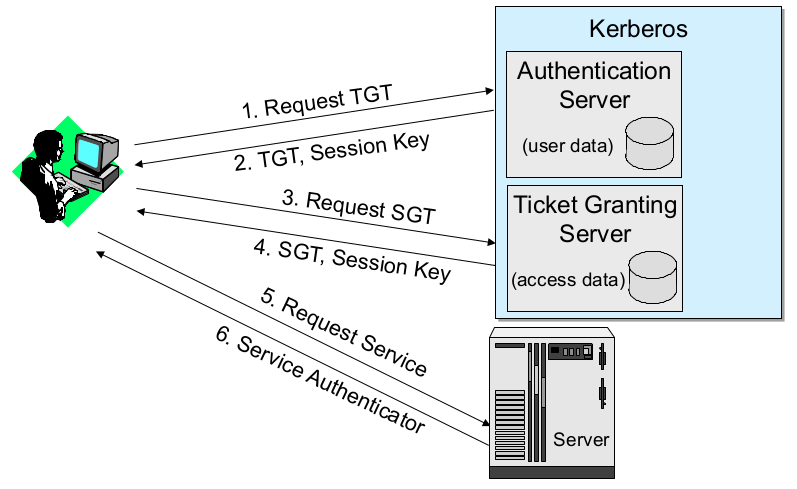
\includegraphics[width=.5\linewidth]{Assets/NetworkSecurity-Kerberos.png}
      \end{center}
      \begin{itemize*}
            \item Der Benutzer meldet sich an seiner Arbeitsstation an und fordert den Zugriff auf einen Dienst an
            \item Die Workstation repräsentiert ihn im Kerberos-Protokoll und sendet die erste Nachricht an den Authentifizierungsserver AS, die seinen Namen, den Namen eines geeigneten Ticket-Granting-Servers TGS und einen Zeitstempel $t_A$ enthält:  $A\rightarrow AS:(A, TGS, t_A)$
            \item Der AS prüft, ob A sich für den Zugang zu den Diensten authentifizieren darf, generiert aus A's Passwort (das ihm bekannt ist) den Schlüssel $K_A$, extrahiert die Arbeitsplatzadresse $Addr_A$ der Anfrage, erstellt ein Ticket $Ticket_{TGS}$ und einen Sitzungsschlüssel $K_{A,TGS}$ und sendet die folgende Nachricht an A: $AS\rightarrow A:\{K_{A,TGS}, TGS, t_{AS}, LifetimeTicket_{TGS}, Ticket_{TGS}\}_{K_A}$ mit $Ticket_{TGS}=\{K_{A,TGS},A, Addr_A, TGS, t_{AS}, LifetimeTicket_{TGS}\}_{K\{AS,TGS\}}$
            \item Nach Erhalt dieser Nachricht fordert die Workstation Alice auf, ihr Passwort einzugeben, berechnet daraus den Schlüssel $K_A$ und entschlüsselt die Nachricht mit diesem Schlüssel. Wenn Alice nicht ihr ,,authentisches'' Passwort angibt, sind die extrahierten Werte ,,Müll'' und der Rest des Protokolls schlägt fehl.
            \item Alice erstellt einen sogenannten Authenticator und sendet ihn zusammen mit dem Ticket und dem Namen des Servers $S1$ an TGS: $A\rightarrow TGS:(S1, Ticket_{TGS}, Authenticator_{A,TGS})$ mit Authenticator $A,TGS=\{A,Addr_A,t'_{A}\}_{K_{A,TGS}}$
            \item Nach Erhalt entschlüsselt TGS $Ticket_{TGS}$, extrahiert daraus den Schlüssel $K_{A,TGS}$ und verwendet diesen Schlüssel zur Entschlüsselung von $Authenticator_{A,TGS}$. Wenn Name und Adresse des Authentifikators und des Tickets übereinstimmen und der Zeitstempel $t_A'$ noch frisch ist, wird geprüft, ob A auf den Dienst S1 zugreifen darf, und die folgende Nachricht erstellt: $TGS\rightarrow A:\{K_{A,S1}, S1, t_{TGS}, Ticket_{S1}\}_{K\{A,TGS\}}$ mit $Ticket_{S1}=\{K_{A,S1}, A, Addr_A, S1, t_{TGS}, LifetimeTicket_{S1}\}_{K\{TGS,S\}}$
            \item Alice entschlüsselt die Nachricht und verfügt nun über einen Sitzungsschlüssel für die sichere Kommunikation mit S1. Sie sendet nun eine Nachricht an S1, um ihm ihr Ticket und einen neuen Authentifikator zu zeigen: $A\rightarrow S1:(Ticket_{S1}, Authenticator_{A,S1})$ mit $Authenticator_{A,S1}=\{A,Addr_A, t''_{A}\}_{K_{A,S1}}$
            \item Nach Erhalt entschlüsselt S1 das Ticket mit dem Schlüssel $K_{TGS,S1}$, den er mit TGS teilt, und erhält den Sitzungsschlüssel $K_{A,S1}$ für die sichere Kommunikation mit A. Mit diesem Schlüssel überprüft er den Authentifikator und antwortet A: $S1\rightarrow A:\{t'\,'_{A+1}\}_{K_{A,S}}$
            \item Durch Entschlüsselung dieser Nachricht und Überprüfung des enthaltenen Wertes kann Alice nachweisen, dass sie wirklich mit S1 kommuniziert, da nur er (neben TGS) den Schlüssel $K_{TGS,S1}$ zur Entschlüsselung von $Ticket_{S1}$ kennt, der den Sitzungsschlüssel $K_{A,S1}$ enthält, und somit nur er in der Lage ist, $Authenticator_{A,S1}$ zu entschlüsseln und mit $t_{A+1}''$ verschlüsselt mit $K_{A,S}$ zu antworten
            \item Das oben beschriebene Protokoll ist der Kerberos-Dialog der Version 4
            \item In diesem Protokoll wurden eine Reihe von Mängeln festgestellt, so dass eine neue Version 5 des Protokolls definiert wurde
      \end{itemize*}

      Kerberos für mehrere Domänen
      \begin{center}
            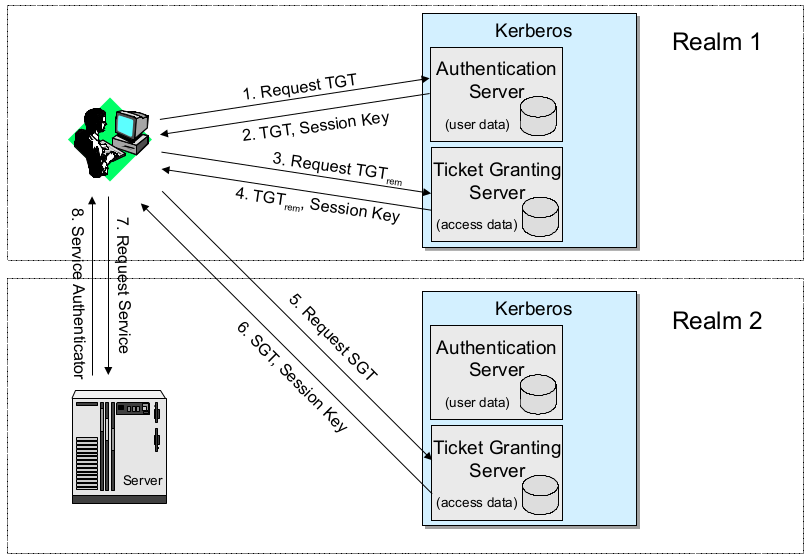
\includegraphics[width=.4\linewidth]{Assets/NetworkSecurity-multi-domain-kerberos.png}
      \end{center}
      \begin{itemize*}
            \item eine Organisation mit Workstation-Clustern an zwei verschiedenen Standorten und Benutzer A von Standort 1 einen Server von Standort 2 benutzen möchte
            \item Wenn beide Standorte ihre eigenen Kerberos-Server und Benutzerdatenbanken (mit Passwörtern) verwenden, gibt es in der Tat zwei verschiedene Domänen, in der Kerberos-Terminologie auch Realms genannt
            \item Um zu vermeiden, dass der Benutzer A in beiden Realms registriert sein muss, ermöglicht Kerberos eine Inter-Realm-Authentifizierung
            \item Die Inter-Realm-Authentifizierung erfordert, dass die Ticket-erteilenden Server beider Domänen einen geheimen Schlüssel $K_{TGS1,TGS2}$ teilen
            \item Die Grundidee ist, dass der TGS eines anderen Realms als normaler Server angesehen wird, für den der TGS des lokalen Realms ein Ticket ausstellen kann
            \item Nachdem Alice das Ticket für den entfernten Realm erhalten hat, fordert sie ein Ticket für den Dienst beim entfernten TGS an
            \item Dies bedeutet jedoch, dass der entfernte Realm dem Kerberos-Authentifizierungsdienst der Heimatdomäne eines ,,besuchenden'' Benutzers vertrauen muss
            \item Skalierbarkeitsproblem: $n$ Realms benötigen $n\times(n-1)/2$ geheime Schlüssel
            \item Nachrichten, die während eines Protokolllaufs mit mehreren Domänen ausgetauscht werden
      \end{itemize*}
      \begin{enumerate*}
            \item $A\rightarrow AS1:(A,TGS1, t_A)$
            \item $AS1\rightarrow A:\{K_{A,TGS1}, TGS1, t_{AS}, LifetimeTicket_{TGS1}, Ticket_{TGS1}\}_{K_A}$ mit $Ticket_{TGS1}=\{K_{A,TGS1}, A, Addr_A, TGS1, t_{AS}, LifetimeTicket_{TGS1}\}_{K\{AS,TGS1\}}$
            \item $A\rightarrow TGS1:(TGS2,Ticket_{TGS1},Authenticator_{A,TGS1})$ mit $Authenticator_{A,TGS1}=\{A,Addr_A,t'_{A}\}_{K_{A,TGS1}}$
            \item $TGS1:\{K_{A,TGS2}, TGS2, t_{TGS1}, Ticket_{TGS2}\}_{K\{A,TGS1\}}$ mit $Ticket_{TGS2}=\{K_{A,TGS2}, A, Addr_A, TGS2, t_{TGS1}, LifetimeTicket_{TGS2}\}_{K\{TGS1,TGS2\}}$
            \item $A\rightarrow TGS2:(S2,Ticket_{TGS2},Authenticator_{A,TGS2})$ mit $Authenticator_{A,TGS2}=\{A,Addr_A,t''_{A}\}_{K_{A,TGS2}}$
            \item $TGS2\rightarrow A:\{K_{A,S2},S2,t_{TGS2},Ticket_{S2}\}_{K\{A,TGS2\}}$ mit $Ticket_{S2}=\{K_{A,S2},A,Addr_A,S2,t_{TGS2}, LifetimeTicket_{S2}\}_{K\{TGS2,S2\}}$
            \item $S2:(Ticket_{S2}, Authentifikator_{A,S2})$ mit $Authentifikator_{A,S2}=\{A,Addr_A,t'''_{A}\}_{K_{A,S2}}$
            \item $S2\rightarrow A:\{t'''_{A+1}\}_{K_{A,S2}}$
      \end{enumerate*}

      \subsubsection{Kerberos Version 5}
      \begin{itemize*}
            \item Letzter Standard von 2005 (RFC 4120)
            \item Entwickelt als Reaktion auf Schwachstellen, die bei Kerberos v4 bekannt wurden
            \item Enthält explizite Prüfsummen, um zu verifizieren, dass die Nachrichten nicht verändert wurden
            \item Unterstützt mehrere Chiffren (andere als das unsichere DES)
            \item Einheitliches Nachrichtenformat - Nachrichten an den Authentifizierungsserver und den Ticketvergabeserver sind sehr ähnlich
            \item Flexible ASN.1-Kodierung der Nachrichten, ermöglicht spätere Erweiterungen
            \item Im Folgenden wird nur eine vereinfachte Version gezeigt, weit mehr Funktionen sind standardisiert, z.B:
            \begin{itemize*}
                  \item Client-zu-Client gegenseitige Authentifizierung
                  \item Vorauthentifizierte Tickets
                  \item Erneuerung von Tickets
                  \item Multidomain Kerberos
            \end{itemize*}
            \item Der Authentifizierungsdialog in Kerberos Version 5 ist ähnlich wie in Version 4
            \item Der Austausch des Authentifizierungsdienstes: Bei der ersten Kontaktaufnahme sendet der Client A nicht nur Namen und Zeitstempel, sondern auch eine Nonce $n$, die hilft, Wiederholungen zu vermeiden, wenn sich die Zeit geändert hat; es ist auch möglich, mehrere Adressen anzugeben $A\rightarrow AS:(A,TGS,t_{start},t_{end},n,Addr_A, ...)$
            \item Die Antwort enthält ein Klartext-Ticket und verschlüsselte Informationen: 2. $AS\rightarrow A: (A,Ticket_{TGS},{K_{A,TGS}, LastRequest,n,t_{expire},t_{AS},t_{start},t_{end},t_{renew},TGS, Addr_A}_{K_A})$ mit $Ticket_{TGS}=(TGS, {K_{A,TGS},A,transited, t_{AS}, t_{start},t_{end},t_{renew},Addr_A,restrictions}_{K\{AS,TGS\}})$
            \begin{itemize*}
                  \item LastRequest gibt den letzten Login des Benutzers an
                  \item transited enthält die Vertrauenskette
                  \item Multidomain Kerberos Restriktionen für den Benutzer können dem TGS und den Servern übergeben werden
                  \item $t_{expire}$ und $t_{end}$ enthalten verschiedene Zeiten, um die Erneuerung von Tickets zu ermöglichen %(wobei die Start- und Endzeit einfach aktualisiert werden können)
            \end{itemize*}
            \item Der Dialog zum TGS ist mit dem Ausgangsdialog harmonisiert: Er enthält zusätzlich Tickets und einen Authentifikator, der beweist, dass A $K_{A,TGS}$ kennt aufrechtes $TGS:(A,S1,t_{start},t_{end},n',Addr_A,Authenticator_{A,TGS}, Tickets,...)$ mit $Authenticator_{A,TGS}=\{A, CheckSum, t_{A'}, K_{A,TGS'}, Seq\#,...\}_{{K}{A,TGS}}$ %Hinweis: Der Authentifikator enthält jetzt eine kryptographische Prüfsumme!
            \item Die Antwort an A ist völlig analog zu Nachricht 2: $TGS\rightarrow A:(A,Ticket_{S1},\{K_{A,S1},LastRequest, n',t_{expire},t_{TGS},t_{start},$ $t_{end},t_{renew},S1,Addr_A\}_{K\{A,TGS\}})$
            \item Der Austausch mit dem Server ist ebenfalls ähnlich wie bei Version 4, aber mit dem Authentifikator ist eine explizite Prüfsumme möglich: $A\rightarrow S1:(Ticket_{S1}, Authenticator_{A,S1})$ mit $Authenticator_{A,S1}=\{A,CheckSum,t_{A''},K_{A,S1}', Seq\#, ...\}_{K\{A,S1\}}$
            \item Nach Erhalt entschlüsselt S1 das Ticket mit dem Schlüssel $K_{TGS,S1}$, den er mit TGS teilt, und erhält den Sitzungsschlüssel $K_{A,S1}$ für die sichere Kommunikation mit A. Mit diesem Schlüssel überprüft er den Authentifikator und antwortet A: $S1\rightarrow A:\{t_{S1},K_{A,S1}',Seq\#,...\}_{K\{A,S1\}}$
            \item Alles in allem behebt der Dialog mehrere potenzielle Schwachstellen, während andere bestehen bleiben
            \begin{itemize*}
                  \item Sequenznummern und Nonces ermöglichen eine zusätzliche Replay-Prüfung, wenn sich die Zeitbasis ändert
                  \item Explizite Prüfsummen verhindern die Änderung von Daten innerhalb von Tickets
                  \item Zentrale Server sind immer noch potentielle Single-Points-of-Failure
                  \item Für den ersten Austausch ist immer noch eine gewisse Zeitsynchronisierung erforderlich
            \end{itemize*}
      \end{itemize*}

      \subsection{Fortgeschrittene Methoden zur Passwortauthentifizierung}
      \begin{itemize*}
            \item Alle gezeigten Protokolle haben eine gemeinsame Schwäche
            \begin{itemize*}
                  \item Passwörter müssen leicht zu merken und leicht einzugeben sein $\rightarrow$ Geringe Entropie
                  \item Angreifer können schnell alle möglichen Kombinationen ausprobieren
                  \item Offline, über Grafikkarten, Cloud-Computer...
                  \item Asymmetrische Situation
            \end{itemize*}
            \item Mögliche Lösungen
            \begin{itemize*}
                  \item Schlüsselableitungsfunktionen
                  \begin{itemize*}
                        \item Erschweren Brute-Force-Angriffe durch extrem häufiges Hashing
                        \item Erfordert auch Aufwand durch legitime Geräte
                        \item Nur linearer Sicherheitsgewinn
                        \item Bessere Funktionen verbrauchen viel Speicher, um Angriffe mit Grafikkarten und spezieller Hardware undurchführbar zu machen
                  \end{itemize*}
                  \item Passwort-authentifizierter Schlüsselaustausch (PAKE)
            \end{itemize*}
            \item Passwortauthentifizierter Schlüsselaustausch (PAKE)
            \begin{itemize*}
                  \item Durchführen eines Schlüsselaustauschs mit asymm. Krypt.
                  \item Authentifizierung von Peers mit einem Passwort unter Verwendung eines Zero Knowledge Proofs
                  \item Die Peers können nur feststellen, ob die Passwörter übereinstimmen oder nicht
                  \item Keine weiteren Informationen, um effiziente Bruteforce-Suchen durchzuführen
                  \item Würde das Lösen schwieriger Probleme erfordern%, z.B. eine Art DH-Problem
                  \item Macht Offline-Angriffe undurchführbar
                  \item Online-Angriffe möglich, können aber entdeckt werden
            \end{itemize*}
      \end{itemize*}

      \subsection{PAKE-Schemata: EKE}
      \begin{itemize*}
            \item ein einfaches erstes Protokoll ist Encrypted Key Exchange (EKE)
            \item Der Dialog beginnt damit, dass A ein Schlüsselpaar zur einmaligen Verwendung erzeugt und den öffentlichen Schlüssel $+K_{ar}$ verschlüsselt mit dem Passwort $K_{A,B}$ an B sendet: $A\rightarrow B:A,\{+K_{ar}\}_{K_{A,B}}$
            \item B wählt einen symmetrischen Sitzungsschlüssel $K_r$ und sendet ihn verschlüsselt mit dem öffentlichen Schlüssel und dem Passwort zurück an A: $B\rightarrow A:{{K_r}_{{+K}{ar}}}_{{K}{A,B}}$
            \item A und B teilen sich nun einen gemeinsamen Sitzungsschlüssel und beweisen ihr Wissen darüber durch den Austausch von Nonces
            \begin{enumerate*}
                  \item $A\rightarrow B:\{r_A\}_{K_r}$
                  \item $B\rightarrow A:\{r_A,r_B\}_{K_r}$
                  \item $A\rightarrow B:\{r_B\}_{K_r}$
            \end{enumerate*}
            \item Nach diesem Schritt ist sichergestellt, dass beide $K_{A,B}$ gekannt haben müssen und es keinen Man-in-the-Middle-Angriff gegeben hat
      \end{itemize*}

      \subsubsection{DH-EKE}
      \begin{itemize*}
            \item DH-EKE ist im Grunde ein DH-Austausch mit Authentifizierung
            \item A sendet DH-Austausch verschlüsselt mit dem Passwort $K_{A,B}$: $A\rightarrow B:\{g^{ra}\ mod\ p\}_{K\{A,B\}}$
            \item B antwortet mit seinem Teil des DH-Austauschs und verwendet den Sitzungsschlüssel $K_S=g^{ra*rb}\ mod\ p$, um eine verschlüsselte Nonce $c_b$ zu senden: $B\rightarrow A:\{g^{rb}\ mod\ p\}_{K\{A,B\}}{c_b}_{K_s}$
            \item Beide Parteien beweisen ihre Kenntnis von $K_S$: $A\rightarrow B:\{c_a|| c_b\}_{K_s}$, $B\rightarrow A:\{c_a\}_{K_s}$
      \end{itemize*}

      \subsubsection{Sicherheitsdiskussion}
      \begin{itemize*}
            \item EKE Resistenz gegen Offline-Angriffe hängt davon ab, dass $+K_{ar}$ nicht von Zufallszahlen zu unterscheiden ist
            \begin{itemize*}
                  \item Für RSA schlagen die Autoren vor, $e$ zu verschlüsseln und $n$ im Klartext zu senden
                  \item $n$ hat keine kleinen Primfaktoren und ist daher von Zufallszahlen unterscheidbar
                  \item Immer noch unsicher gegen Man-in-the-Middle-Angriffe, da Angreifer $n$ mit besonderen Eigenschaften wählen können %(z.B. $p-1$ und $q-1$ teilbar durch 3)
                  \item Antwort von B ist von Zufallszahlen unterscheidbar
                  \item Bietet keine perfekte Vorwärtsverschwiegenheit...
            \end{itemize*}
            \item Protokoll DH-EKE
            \begin{itemize*}
                  \item Der Wert p muss klug gewählt werden, d.h. $p-1$ muss nahe bei $2^{8*n}$ für ausreichend große natürliche Zahlen $n$ liegen
                  \item Um Angriffe auf kleine Gruppen leicht zu verhindern, sollte $(p-1)/2$ ebenfalls eine Primzahl sein
                  \item ECC ist immer noch schwierig zu realisieren
                  \item Bietet perfektes Vorwärtsgeheimnis
                  \item Alles in allem ein nettes Verfahren, das jedoch patentiert werden musste
                  \begin{itemize*}
                        \item Keine breite Anpassung
                        \item Führte zur Entwicklung zahlreicher anderer Verfahren
                  \end{itemize*}
            \end{itemize*}
      \end{itemize*}

      \subsubsection{Secure Remote Password (SRP)}
      \begin{itemize*}
            \item heute am weitesten verbreitete Protokoll (hier SRP-6a)
            \item Initialisierung
            \begin{itemize*}
                  \item Server B wählt eine Zufallszahl $s_{A,B}$
                  \item berechnet $x=H(s_{A,B} || Benutzername || Passwort)$ und $v=g^x\ mod\ p$
                  \item Benutzer werden durch $(Benutzername, s_{A,B}, v)$ authentifiziert
                  \item Der Server braucht das Passwort nicht zu speichern $\rightarrow$ kann nicht leicht erlangt werden, wenn der Server kompromittiert wird
                  \item Server kann diese Werte auch nicht verwenden, um sich als Benutzer auf anderen Servern auszugeben
                  \item Die Eigenschaft wird als erweitertes PAKE-Schema bezeichnet
            \end{itemize*}
      \end{itemize*}

      SRP-Dialog
      \begin{itemize*}
            \item A initiiert die Verbindung durch Senden seines Benutzernamens $A\rightarrow B: A$
            \item B antwortet mit ausgewählten kryptographischen Parametern und einem Verifizierer v, der durch einen DH-Austausch geblendet ist: $B\rightarrow A: p, g, s_{A,B}, (H(g || p)*v + g^{rb})\ mod\ p$
            \item A berechnet den gemeinsamen Sitzungsschlüssel durch $K_S=(Y_B-H(g || p)_{g^{ra+u}})\ mod\ p$, mit $u=H(Y_A||Y_B)$, und sendet seinen Teil des DH-Austauschs und eine Bestätigung zurück, dass er $K_S$ kennt $A\rightarrow B:g^{ra}\ mod\ p, H(Y_A,Y_B,K_S)$
            \item B berechnet $K_S'=(Y_A v^u)^{rb}\ mod\ p$ und beweist seine Kenntnis $B\rightarrow A:H(Y_A, H(Y_A,Y_B,K_S),K_S')$
            \item $K_S'$ und $K_S$ stimmen überein, wenn es keinen Man-in-the-Middle-Angriff gegeben hat
      \end{itemize*}

      SRP-Diskussion
      \begin{itemize*}
            \item Sicheres Schema
            \item Gegenseitige Authentifizierung zwischen Server und Client
            \item Erweiterung erhöht die Sicherheit in Client/Server-Szenarien
            \item Keine Unterstützung für ECC, da es Feldarithmetik erfordert
            \item Patentiert aber frei zu verwenden
            \item Unterstützung für TLS, IPsec, ...
      \end{itemize*}

      \subsection{X.509 - Einführung}
      \begin{itemize*}
            \item X.509 ist eine internationale Empfehlung der ITU-T %und gehört zur X.500-Reihe, die Verzeichnisdienste definiert:
            %\begin{itemize*}
            %      \item Die erste Version von X.509 wurde 1988 standardisiert.
            %      \item Eine zweite Version, die 1993 standardisiert wurde, löste einige Sicherheitsbedenken
            %      \item Eine dritte Version von X.509 wird derzeit von der IETF in RFC 4211 gepflegt.
            %\end{itemize*}
            \item X.509 definiert einen Rahmen für die Bereitstellung von Authentifizierungsdiensten, der Folgendes umfasst
            \item Zertifizierung von öffentlichen Schlüsseln und Handhabung von Zertifikaten
            \begin{itemize*}
                  \item Zertifikatsformat
                  \item Zertifikats-Hierarchie
                  \item Zertifikatswiderrufslisten
            \end{itemize*}
            \item Drei verschiedene Dialoge für die direkte Authentifizierung
            \begin{itemize*}
                  \item Einseitige Authentifizierung, erfordert synchronisierte Uhren
                  \item Gegenseitige Zwei-Wege-Authentifizierung, erfordert immer noch synchronisierte Uhren
                  \item Gegenseitige Drei-Wege-Authentifizierung, die vollständig auf Zufallszahlen basiert
            \end{itemize*}
      \end{itemize*}

      \subsubsection{X.509 - Zertifikate mit öffentlichem Schlüssel}
      \begin{multicols}{2}
            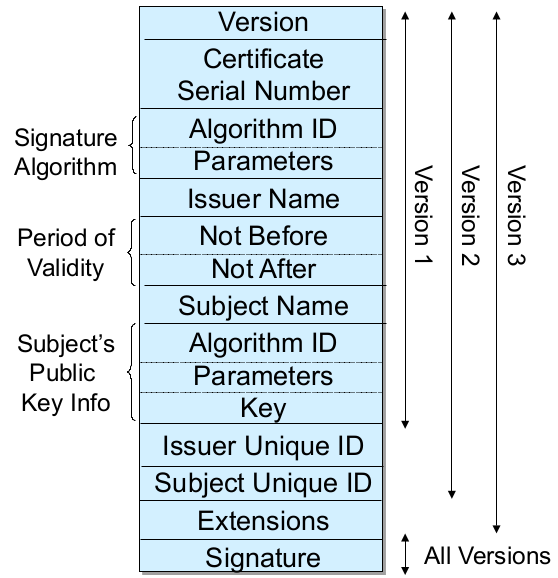
\includegraphics[width=\linewidth]{Assets/NetworkSecurity-x509-certificates.png}
            \columnbreak

            \begin{itemize*}
                  \item Ein Public-Key-Zertifikat ist eine Art Reisepass, der bescheinigt, dass ein öffentlicher Schlüssel zu einem bestimmten Namen gehört
                  \item Zertifikate werden von Zertifizierungsstellen (CA) ausgestellt
                  \item Wenn alle Nutzer den öffentlichen Schlüssel der CA kennen, kann jeder Nutzer jedes von dieser CA ausgestellte Zertifikat überprüfen
                  \item Zertifikate können die Online-Teilnahme eines TTP verhindern
                  \item Die Sicherheit des privaten Schlüssels der CA ist entscheidend für die Sicherheit aller Nutzer
            \end{itemize*}
      \end{multicols}

      \begin{itemize*}
            \item Notation eines Zertifikats, das einen öffentlichen Schlüssel $+K_A$ an Benutzer A bindet, ausgestellt von der Zertifizierungsstelle CA unter Verwendung ihres privaten Schlüssels $-CK_{CA}$:
            \item $Cert_{-CK_{CA}}(+K_A) = CA_{V, SN, AI, CA, T_{CA}, A, +K_A}$ mit:
            \begin{itemize*}
                  \item V = Versionsnummer
                  \item SN = Seriennummer
                  \item AI = Algorithmus-Bezeichner des verwendeten Signatur-Algorithmus
                  \item CA = Name der Zertifizierungsstelle
                  \item $T_{CA}$ = Gültigkeitsdauer dieses Zertifikats
                  \item A = Name, an den der öffentliche Schlüssel in diesem Zertifikat gebunden ist
                  \item $+K_A$ = öffentlicher Schlüssel, der an einen Namen gebunden wird
            \end{itemize*}
            \item Die Kurzschreibweise $CA_m$ steht für $(m,{H(m)}_{{-CK}{CA}})$
            \item Eine andere Kurzschreibweise für $Cert_{-CK_{CA}}(+K_A)$ ist $CA<>$
      \end{itemize*}

      \subsubsection{X.509 - Zertifikatsketten \& Zertifikatshierarchie}
      \begin{itemize*}
            \item Betrachten wir nun zwei Benutzer A und B die sicher kommunizieren wollen
            \begin{itemize*}
                  \item Die Wahrscheinlichkeit ist recht hoch, dass ihre öffentlichen Schlüssel von verschiedenen CAs zertifiziert sind
                  \item Nennen wir die Zertifizierungsstelle von A CA und die von B CB
                  \item Wenn A CB nicht vertraut oder gar kennt, dann ist Bs Zertifikat $CB<>$ für sie nutzlos, dasselbe gilt in der anderen Richtung
            \end{itemize*}
            \item Eine Lösung für dieses Problem ist die Konstruktion von Zertifikatsketten
            \begin{itemize*}
                  \item CA und CB kennen und vertrauen einander
                  %\item Ein Beispiel aus der realen Welt für dieses Konzept ist das gegenseitige Vertrauen zwischen Ländern hinsichtlich ihrer Passausgabestellen
                  \item Wenn CA den öffentlichen Schlüssel von CB mit einem Zertifikat $CA<>$ und CB den öffentlichen Schlüssel von CA mit einem Zertifikat $CB<>$ beglaubigt, können A und B ihre Zertifikate anhand einer Zertifikatskette überprüfen
                  \item Nachdem ihr $CB<>$ vorgelegt wurde, versucht A herauszufinden, ob es ein Zertifikat $CA<>$ gibt.
                  \item Sie überprüft dann die Kette: $CA<>, CB<>$
            \end{itemize*}
            \item Zertifikatsketten müssen nicht auf eine Länge von zwei Zertifikaten beschränkt sein
            %\begin{itemize*}
            %      \item $CA<>, CC<>, CD<>, CE<>, CG<>$ würde es Alice erlauben, das von CG ausgestellte Zertifikat des Benutzers G zu überprüfen, auch wenn sie nur ihre eigene Zertifizierungsstelle CA kennt und ihr vertraut.
            %      \item Tatsächlich wird das Vertrauen von A in den Schlüssel +KG durch eine Vertrauenskette zwischen Zertifizierungsstellen hergestellt.
            %      \item Wenn Alice jedoch $CG<>$ vorgelegt wird, ist es nicht offensichtlich, welche Zertifikate sie zur Überprüfung benötigt
            %\end{itemize*}
            \item X.509 schlägt daher vor, dass die Zertifizierungsstellen in einer Zertifizierungshierarchie angeordnet werden, so dass die Navigation einfach ist
            \item 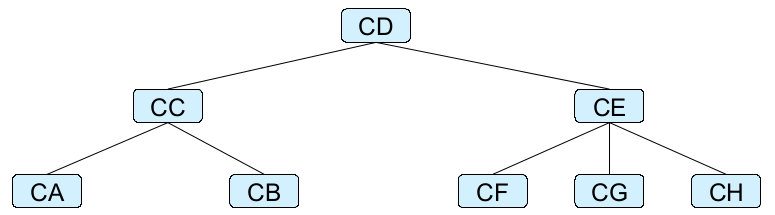
\includegraphics[width=.5\linewidth]{Assets/NetworkSecurity-x509-hierarchy.png}
            \item Verbleibendes Problem
            \begin{itemize*}
                  \item Zertifizierungspfade können ziemlich lang werden
                  \item die Kompromittierung eines einzigen Zwischenzertifikats reicht aus, um die Sicherheit zu brechen
                  \item Führt zu zwei Entwicklungen
            \end{itemize*}
      \end{itemize*}
      \begin{description*}
            \item[Kreuzzertifizierung]
            \begin{itemize*}
                  \item Ermöglicht das Signieren von Stammzertifikaten untereinander
                  \item Erlaubt aber auch ,,Abkürzungen'' im Zertifikatswald
                  \item Macht die Navigation komplexer aber potenziell mehrwegfähig
            \end{itemize*}
            \item[Anheften von Zertifikaten] Ermöglicht Anwendungen zu lernen, dass Peers nur Zertifikate von einer bestimmten CA verwenden. Wird z.B. von Google Chrome verwendet%, nachdem Man-in-the-Middle-Angriffe auf google.com bekannt wurden
      \end{description*}

      \subsubsection{X.509 - Zertifikatssperrung}
      \begin{itemize*}
            \item privater Schlüssel von A kompromittiert
            \begin{itemize*}
                  \item Wenn A feststellt, dass ihr privater Schlüssel kompromittiert wurde, möchte sie unbedingt den Widerruf des entsprechenden Zertifikats für den öffentlichen Schlüssel beantragen
                  \item Wenn das Zertifikat nicht widerrufen wird, könnte sich E bis zum Ende der Gültigkeitsdauer des Zertifikats weiterhin als A ausgeben.
            \end{itemize*}
            \item Eine noch schlimmere Situation tritt ein, wenn der private Schlüssel einer Zertifizierungsstelle kompromittiert wird $\rightarrow$ alle mit diesem Schlüssel signierten Zertifikate müssen widerrufen werden
            \item Der Widerruf von Zertifikaten wird durch das Führen von Zertifikatswiderrufslisten (CRL) realisiert
            \begin{itemize*}
                  \item CRLs werden im X.500-Verzeichnis gespeichert oder Erweiterungen können auf eine URL verweisen
                  \item Bei der Überprüfung eines Zertifikats muss auch geprüft werden, ob das Zertifikat noch nicht widerrufen wurde %(Suche nach dem Zertifikat in der CRL)
                  \item Der Widerruf von Zertifikaten ist ein relativ langsamer und teurer Vorgang
            \end{itemize*}
      \end{itemize*}

      \subsubsection{X.509 - Authentifizierungsprotokolle}
      \begin{itemize*}
            \item Einweg-Authentifizierung
            \begin{itemize*}
                  \item Wenn nur Alice sich gegenüber Bob authentifizieren will, sendet sie folgende Nachricht an Bob: $(A[t_A, r_A, B, sgnData_A, {K_{A,B}}_{+KB}], CA<>)$,
                  \item wobei $sgnData_A$ optionale Daten darstellt, die von A signiert werden sollen,
                  \item $K\{A,B\}_{+K_B}$ ein optionaler Sitzungsschlüssel ist, der mit Bobs öffentlichem Schlüssel verschlüsselt wird,
                  \item $CA<>$ ebenfalls optional
                  \item Beim Empfang dieser Nachricht verifiziert Bob mit $+K_{CA}$ das enthaltene Zertifikat, extrahiert Alices öffentlichen Schlüssel, überprüft Alices Signatur der Nachricht und die Aktualität der Nachricht $(t_A)$ und entschlüsselt optional den enthaltenen Sitzungsschlüssel $K_{A,B}$, den Alice vorgeschlagen hat
            \end{itemize*}
            \item Zwei-Wege-Authentifizierung
            \begin{itemize*}
                  \item Wenn eine gegenseitige Authentifizierung erwünscht ist, dann erstellt Bob eine ähnliche Nachricht
                  \item $(B,,t_B, r_B, A, r_A, sgnData_B,{K_{B,A}}_{+K_A}'', CA<>)$
                  \item der enthaltene Zeitstempel $t_B$ ist nicht wirklich erforderlich, da Alice überprüfen kann, ob die signierte Nachricht die Zufallszahl $r_A$ enthält
            \end{itemize*}
            \item Drei-Wege-Authentifizierung
            \begin{itemize*}
                  \item Wenn Alice und Bob nicht sicher sind, ob sie synchrone Uhren haben, sendet Alice die folgende Nachricht an Bob: $A[r_B]$
                  \item Die Rechtzeitigkeit der Teilnahme von Alice am Authentifizierungsdialog wird also durch die Unterzeichnung der ,,frischen'' Zufallszahl $r_B$ nachgewiesen
            \end{itemize*}
            \item Anmerkung zum Signaturalgorithmus
            \begin{itemize*}
                  \item Wie aus der Verwendung von Zertifikaten ersichtlich, schlägt X.509 vor, die Authentifizierungsnachrichten mit asymmetrischer Kryptographie zu signieren
                  \item Das Authentifizierungsprotokoll selbst kann jedoch auch mit symmetrischer Kryptographie eingesetzt werden
                  \item In diesem Fall müssen sich A und B vor jedem Protokolldurchlauf auf einen geheimen Authentifizierungsschlüssel $AK_{A,B}$ geeinigt haben, und
                  \item die Nachrichten werden durch Anhängen eines mit diesem Schlüssel berechneten MAC signiert
            \end{itemize*}
      \end{itemize*}

      \subsection{Formale Validierung von krypt. Protokollen}
      Kategorien von formalen Validierungsmethoden für kryptografische Protokolle
      \begin{itemize*}
            \item Allgemeine Ansätze zur Analyse spezifischer Protokolleigenschaften:
            \begin{itemize*}
                  \item Beispiele: Finite-State-Machine-basierte Ansätze, Prädikatenkalkül %erster Ordnung, Allzweck-Spezifikationssprachen
                  \item Hauptnachteil: Sicherheit unterscheidet sich wesentlich von Korrektheit, da für letztere keine böswillige Manipulation angenommen werden muss
            \end{itemize*}
            \item Expertensystembasierte Ansätze
            \begin{itemize*}
                  \item Das Wissen menschlicher Experten wird in deduktive Regeln formalisiert, die von einem Protokolldesigner zur Untersuchung verschiedener Szenarien verwendet werden können.
                  \item Hauptnachteil: nicht gut geeignet, um Schwachstellen in kryptografischen Protokollen zu finden, die auf unbekannten Angriffstechniken beruhen
            \end{itemize*}
            \item Algebraische Ansätze
            \begin{itemize*}
                  \item Kryptografische Protokolle werden als algebraische Systeme spezifiziert
                  \item Die Analyse wird durchgeführt, indem algebraische Termumschreibungseigenschaften des Modells untersucht werden und geprüft wird, ob das Modell bestimmte erwünschte oder unerwünschte Zustände erreichen kann
            \end{itemize*}
            \item Spezifische logikbasierte Ansätze
            \begin{itemize*}
                  \item Ansätze dieser Klasse definieren einen Satz von Prädikaten und eine Abbildung der während eines Protokolllaufs ausgetauschten Nachrichten auf einen Satz von Formeln
                  \item Ein generischer Satz von Regeln erlaubt es dann, das Wissen und den Glauben zu analysieren, der von den Peer-Entitäten eines kryptographischen Protokolls während eines Protokolllaufs erlangt wird %(recht erfolgreicher Ansatz: GNY-Logik)
            \end{itemize*}
      \end{itemize*}
      \columnbreak

      \section{Zugriffskontrolle}
      \subsection{Was ist Zugangskontrolle?}
      \begin{itemize*}
            \item Die Zugriffskontrolle umfasst die Mechanismen, die die Vermittlung von Subjektanfragen für den Zugriff auf Objekte, wie sie in einer bestimmten Sicherheitspolitik definiert sind, erzwingen.
            \item wichtiges konzeptuelles Modell ist der Referenzmonitor
            %\item 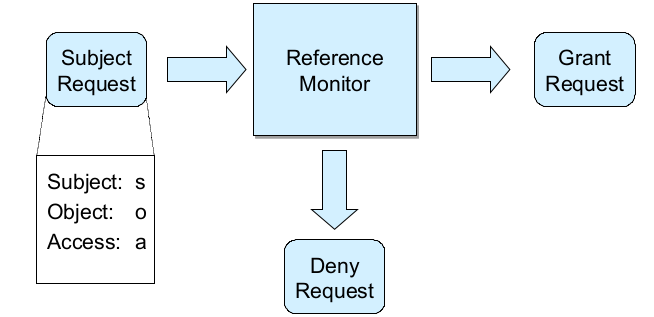
\includegraphics[width=\linewidth]{Assets/NetworkSecurity-reference-monitor.png}
      \end{itemize*}

      \subsection{Sicherheitspolitik}
      \begin{itemize*}
            \item Um Entscheidungen über die Zugriffskontrolle treffen zu können, muss der Referenzmonitor die Sicherheitspolitik des Systems kennen
            \item Die \textbf{Sicherheitspolitik} eines Systems definiert die Bedingungen, unter denen Subjektzugriffe auf Objekte durch die Funktionalität des Systemreferenzmonitors vermittelt werden
            \item wird gewöhnlich im Zusammenhang mit der Sicherheit von Computern und Betriebssystemen gegeben
            \item Referenzmonitor ist nur eine konzeptionelle Einheit%, er muss nicht unbedingt ein physisches oder logisches Gegenstück in einem bestimmten System haben
            \item Der Begriff Sicherheitspolitik wird oft auch in einem weiteren Sinne verwendet, um eine Spezifikation aller Sicherheitsaspekte eines Systems einschließlich Bedrohungen, Risiken, Sicherheitsziele, Gegenmaßnahmen usw. zu beschreiben
      \end{itemize*}

      \subsection{Klassische Subjekte, Objekte und Zugriffsarten}
      \begin{itemize*}
            \item Ein Subjekt ist eine aktive Entität, die eine Anfrage nach Ressourcen initiieren und diese Ressourcen nutzen kann, um eine Aufgabe zu erfüllen
            \item Ein Objekt ist ein passives Repository, das zur Speicherung von Informationen dient
            \item Die beiden obigen Definitionen stammen aus der klassischen Computerwissenschaft
            %\item Subjekte sind Prozesse, und Dateien, Verzeichnisse usw. sind Objekte
            \item Es ist jedoch nicht immer offensichtlich, Subjekte und Objekte im Zusammenhang mit der Kommunikation zu identifizieren
            %\item Stellen Sie sich vor, eine Einheit sendet eine Nachricht an eine andere Einheit: Ist die empfangende Einheit als Objekt zu betrachten?
            \item Außerdem muss man wissen, was ein Zugriff ist und welche Arten von Zugriffen es gibt
            \item Beispiele aus der klassischen Informatik für Zugriffsarten: Lesen, Schreiben, Ausführen
            %\item Objektorientierte Sichtweise: Jede Methode eines Objekts definiert eine Art des Zugriffs
      \end{itemize*}

      \subsection{Sicherheitskennzeichen}
      \begin{itemize*}
            \item \textbf{Sicherheitsstufe} wird als hierarchisches Attribut zu Entitäten eines Systems definiert, um deren Sensibilitätsgrad zu kennzeichnen
            \begin{itemize*}
                  \item Militär: unklassifiziert $<$ vertraulich $<$ geheim
                  \item Kommerziell: öffentlich $<$ sensibel $<$ eingeschränkt
            \end{itemize*}
            \item \textbf{Sicherheitskategorie} definiert als nicht-hierarchische Gruppierung von Entitäten, um den Grad ihrer Sensibilität zu kennzeichnen
            \begin{itemize*}
                  \item Beispiel: Abteilung A, Abteilung B, Verwaltung usw.
            \end{itemize*}
            \item \textbf{Sicherheitskennzeichnung} definiert als Attribut, das mit Systemeinheiten verbunden ist, um deren hierarchische Sensibilitätsstufe und Sicherheitskategorien zu kennzeichnen.
            \begin{itemize*}
                  \item In Form von mathematischen Mengen: $Labels = Levels \times Powerset(Categories)$
            \end{itemize*}
            \item Sicherheitslabels, die die Sicherheitsempfindlichkeit von
            \begin{itemize*}
                  \item Subjekte werden Freigaben genannt
                  \item Objekte werden Klassifizierungen genannt
            \end{itemize*}
            \item Ein wichtiges Konzept für die Spezifikation von Sicherheitspolitiken sind binäre Relationen auf der Menge der Kennzeichnungen: Eine binäre Relation auf einer Menge S ist eine Teilmenge des Kreuzprodukts $S\times S$
            %\begin{itemize*}
            %      \item Dominiert: $Labels \times Labels$
            %      \item Dominiert $={(b1,b2) | b1, b2 \in Labels \wedge level(b1) \geq level(b2) \wedge categories(b2) \subseteq categories(b1)}$
            %      \item Wenn $(b1, b2) \in Dominates$, schreiben wir auch b1 dominates b
            %\end{itemize*}
      \end{itemize*}

      \subsection{Spezifikation der Sicherheitspolitik}
      \begin{itemize*}
            \item Formale Ausdrücke für Regeln der Sicherheitspolitik
            \item Betrachten Sie die folgenden Zuordnungen
            \begin{itemize*}
                  \item $allow: Subjects \times Accesses \times Objects \rightarrow boolean$
                  \item $own: Subjects \times Objects \rightarrow boolean$
                  \item $admin: Subjects \rightarrow boolean$
                  \item $dominates: Labels \times Labels \rightarrow boolean$
            \end{itemize*}
            \item Die oben genannten Zuordnungen können verwendet werden, um bekannte Sicherheitsrichtlinien zu spezifizieren
            \begin{itemize*}
                  \item $ownership: \forall s \in Subjects, o \in Objects, a \in Accesses: allow(s, o, a) \Leftrightarrow own(s, o)$
                  \item $own_admin: \forall s \in Subjects, o \in Objects, a \in Accesses: allow(s, o, a) \Leftrightarrow own(s, o) \wedge admin(s)$
                  \item $dom: \forall s \in Subjects, o \in Objects, a \in Accesses: allow(s, o, a) \Leftrightarrow dominates(label(s), label(o))$
            \end{itemize*}
            \item Die dom-Policy erfordert ein System zur Speicherung und Verarbeitung von Sicherheitskennzeichnungen für jede Entität, erlaubt aber komplexere Zugriffskontrollschemata als die ownership- und own\_admin-Policy
      \end{itemize*}

      \subsection{Arten von Zugriffskontrollmechanismen}
      \begin{itemize*}
            \item Ein Zugriffskontrollmechanismus ist eine konkrete Umsetzung des Referenzmonitor-Konzepts
            \item Es gibt zwei Haupttypen von Zugriffskontrollmechanismen:
            \begin{description*}
                  \item[Diskretionäre Zugriffskontrolle] umfasst diejenigen Verfahren und Mechanismen, die die spezifizierte Vermittlung nach dem Ermessen der einzelnen Benutzer durchsetzen
                  %\item Beispiel: Das Unix-Betriebssystem ermöglicht es den Benutzern, die Zugriffsrechte für Dateien, die ihnen gehören, zu erteilen oder zu entziehen (Lesen, Schreiben, Ausführen).
                  \item[obligatorische Zugriffskontrolle] umfasst die Verfahren und Mechanismen, die die angegebene Vermittlung nach dem Ermessen einer zentralen Systemverwaltung durchsetzen.
            \end{description*}
            \item Beide Arten können kombiniert werden, wobei die obligatorischen Zugriffskontrollentscheidungen in den meisten Fällen Vorrang vor den diskretionären Entscheidungen haben
            %\item Beispiel: Verwendung einer diskretionären Zugangskontrolle auf Personalcomputern kombiniert mit einer obligatorischen Zugangskontrolle für die Kommunikation ($\rightarrow$ Firewalls)
      \end{itemize*}

      \subsection{Zugriffsmatrizen}
      \begin{itemize*}
            \item Ein nützliches Konzept für die Beschreibung von Zugangskontrollmechanismen ist die Zugangsmatrix
            \item In einer Zugriffsmatrix für zwei Mengen von Subjekten und Objekten entspricht jede Zeile einem Subjekt und jede Spalte einem Objekt
            \item Jede Zelle der Matrix definiert die Zugriffsrechte des entsprechenden Subjekts auf das entsprechende Objekt
      \end{itemize*}

      %\begin{longtable}[]{@{}lllll@{}}
      % \toprule
      % & Object 1 & Object 2 & ... & Object M\tabularnewline
      % \midrule
      % \endhead
      % Subject 1 & & & ... & \tabularnewline
      % Subject 2 & & & ... & \tabularnewline
      % ... & ... & ... & (Access Rights) & \tabularnewline
      % Subject N & & & & \tabularnewline
      % \bottomrule
      %\end{longtable}

      \subsection{Gemeinsame Zugriffskontrollschemata}
      \begin{itemize*}
            \item Zugriffskontroll-Listen (ACL)
            \begin{itemize*}
                  \item Grundlage für Zugriffskontrollschema, bei dem für jedes Objekt eine Liste gültiger Subjekte gespeichert wird, die Zugriff auf dieses Objekt haben könnten %(möglicherweise zusammen mit der Art des erlaubten Zugriffs)
                  \item in der Regel bei der diskretionären Zugriffskontrolle verwendet, da es zu viele ACLs gibt, als dass sie von einer zentralen Verwaltungseinrichtung verwaltet werden könnten
            \end{itemize*}
            \item Capabilities
            \begin{itemize*}
                  \item gewissermaßen das Gegenkonzept zu ACLs, da bei Capabilities jedes Subjekt eine Liste von Zugriffsrechten auf Objekte besitzt
                  \item Der Vorteil ist, dass ein Subjekt einige seiner Capabilities an andere Subjekte weitergeben kann
            \end{itemize*}
            \item Label-basierte Zugriffskontrolle
            \begin{itemize*}
                  \item Wenn Sicherheitslabels mit den Entitäten eines Systems gespeichert und verarbeitet werden, können sie zur Durchführung einer label-basierten Zugriffskontrolle verwendet werden
                  \item Dieses Verfahren wird in der Regel als obligatorischer Zugriffskontrollmechanismus verwendet
            \end{itemize*}
            \item[$\rightarrow$] die Datenintegrität von Zugriffskontrolldatenstrukturen ist entscheidend
      \end{itemize*}
      \columnbreak

      \section{Integration von Sicherheitsdiensten in Kommunikationsarchitekturen}
      \subsection{Motivation: Was ist wo zu tun?}
      \begin{itemize*}
            \item Analog zur Methodik der Sicherheitsanalyse gibt es zwei Dimensionen, die bei der Integration von Sicherheitsdiensten in Kommunikationsarchitekturen zu beachten sind:
            \item Dimension 1: Welcher Sicherheitsdienst soll in welchem Knoten realisiert werden?
            % \item 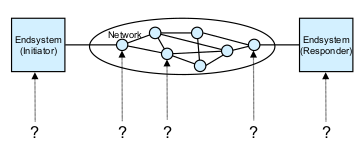
\includegraphics[width=\linewidth]{Assets/NetworkSecurity-Security-service-dim-1.png}
            \item Dimension 2: Welcher Sicherheitsdienst sollte in welcher Schicht realisiert werden?
            % \item 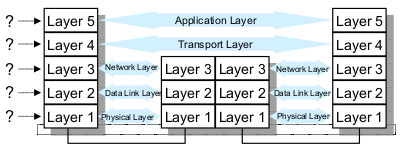
\includegraphics[width=\linewidth]{Assets/NetworkSecurity-Security-service-dim-2.png}
      \end{itemize*}

      \subsection{Ein pragmatisches Modell für sicheres und vernetztes Rechnen}
      \begin{itemize*}
            %\item \includegraphics[width=\linewidth]{Assets/NetworkSecurity-Sicheres-Netz-Modell.png}
            \item Anwendung: Ein Stück Software, das eine bestimmte Aufgabe erfüllt, z.B. elektronische E-Mail, Webdienst, Textverarbeitung, Datenspeicherung usw.
            \item Endsystem:
            \begin{itemize*}
                  \item Ein Gerät, das vom Personal Computer über den Server bis zum Großrechner reicht.
                  \item Für Sicherheitszwecke hat ein Endsystem in der Regel eine einzige Richtlinienautorität.
            \end{itemize*}
            \item Teilnetz:
            \begin{itemize*}
                  \item Eine Sammlung von Kommunikationseinrichtungen, die unter der Kontrolle einer Verwaltungsorganisation stehen, z.B. ein LAN, ein Campusnetz, ein WAN usw.
                  \item Für Sicherheitszwecke hat ein Teilnetz in der Regel eine Richtlinienkompetenz.
            \end{itemize*}
            \item Internet:
            \begin{itemize*}
                  \item Eine Sammlung von miteinander verbundenen Teilnetzen
                  \item Im Allgemeinen haben die Teilnetze, die in einem Inter-Netzwerk verbunden sind, unterschiedliche Richtlinienautoritäten
            \end{itemize*}
            \item Es gibt vier Ebenen, auf denen unterschiedliche Anforderungen an Sicherheitsprotokollelemente gestellt werden:
            \begin{itemize*}
                  \item Anwendungsebene: Sicherheitsprotokollelemente, die anwendungsabhängig sind
                  \item Endsystem-Ebene: Bereitstellung von Schutz auf einer Endsystem-zu-Endsystem-Basis
                  \item Teilnetzebene: Bereitstellung von Schutz über ein Teilnetz oder ein Zwischennetz, das als weniger sicher gilt als andere Teile der Netzumgebung
                  \item Verbindungsebene: Bereitstellung von Schutz innerhalb eines Teilnetzes, z.B. über eine Verbindung, die als weniger vertrauenswürdig gilt als andere Teile der Teilnetzumgebung
            \end{itemize*}
      \end{itemize*}

      \subsection{Beziehungen zwischen Schichten und Anforderungsniveaus}
      \begin{itemize*}
            \item Die Beziehungen zwischen den Protokollschichten und den Stufen der Sicherheitsanforderungen für die Protokollelemente sind nicht eins-zu-eins
            \item Sicherheitsmechanismen, die sowohl die Anforderungen der Endsystem- als auch der Teilnetzebene erfüllen, können entweder in der Transport- und/oder in der Netzwerkschicht realisiert werden.
            \item Die Anforderungen der Verbindungsebene können durch die Integration von Sicherheitsmechanismen oder durch die Verwendung von ,,speziellen Funktionen'' der Verbindungsschicht und/oder der physikalischen Schicht erfüllt werden.
            % \item 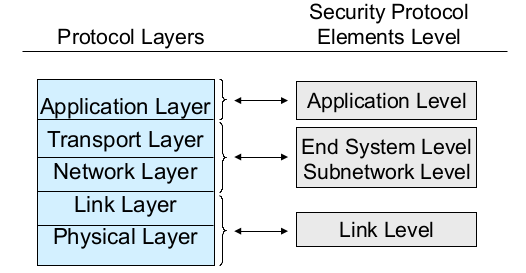
\includegraphics[width=\linewidth]{Assets/NetworkSecurity-Layer-relationship.png}
      \end{itemize*}

      \subsection{Allgemeine Überlegungen zur architektonischen Platzierung}
      \begin{itemize*}
            \item Verkehrsvermischung:
            \begin{itemize*}
                  \item Infolge des Multiplexing besteht auf niedrigeren Ebenen eine größere Tendenz, Datenelemente von verschiedenen Quell-/Ziel-Benutzern und/oder Anwendungen in einem Datenstrom zu vermischen
                  \item Ein Sicherheitsdienst, der auf einer Schicht/Ebene realisiert wird, behandelt den Verkehr dieser Schicht/Ebene gleich, was zu einer unzureichenden Kontrolle der Sicherheitsmechanismen für Benutzer und Anwendungen führt.
                  \item Wenn eine Sicherheitspolitik eine differenziertere Behandlung erfordert, sollte sie besser auf einer höheren Ebene realisiert werden
            \end{itemize*}
            \item Wissen über die Route:
            \begin{itemize*}
                  \item Auf niedrigeren Ebenen ist in der Regel mehr Wissen über die Sicherheitseigenschaften der verschiedenen Routen und Verbindungen vorhanden.
                  \item In Umgebungen, in denen diese Merkmale stark variieren, kann die Platzierung von Sicherheit auf niedrigeren Ebenen Vorteile in Bezug auf Effektivität und Effizienz haben
                  \item Geeignete Sicherheitsdienste können auf der Basis von Teilnetzen oder Verbindungen ausgewählt werden, so dass keine Kosten für Sicherheit anfallen, wenn der Schutz unnötig ist.
            \end{itemize*}
            \item Anzahl der Schutzpunkte:
            \begin{itemize*}
                  \item Wenn die Sicherheit auf der Anwendungsebene angesiedelt wird, muss die Sicherheit in jeder sensiblen Anwendung und jedem Endsystem implementiert werden.
                  \item Sicherheit auf der Verbindungsebene bedeutet, dass am Ende jeder Netzverbindung, die als weniger vertrauenswürdig gilt, Sicherheit implementiert werden muss.
                  \item Wenn die Sicherheit in der Mitte der Architektur angesiedelt wird, müssen die Sicherheitsmerkmale an weniger Stellen installiert werden.
            \end{itemize*}
            \item Schutz der Protokoll-Header:
            \begin{itemize*}
                  \item Der Sicherheitsschutz auf höheren Ebenen kann die Protokollköpfe der unteren Protokollschichten nicht schützen.
                  \item Die Netzwerkinfrastruktur muss möglicherweise ebenfalls geschützt werden.
            \end{itemize*}
            \item Quelle/Senke-Bindung:
            \begin{itemize*}
                  \item Sicherheitsdienste wie die Authentifizierung der Datenherkunft und die Unleugbarkeit hängen von der Zuordnung der Daten zu ihrer Quelle oder Senke ab.
                  \item Dies wird am effizientesten auf höheren Ebenen erreicht, insbesondere auf der Anwendungsebene.
            \end{itemize*}
      \end{itemize*}

      \subsection{Überlegungen zu bestimmten Ebenen}
      \begin{itemize*}
            \item Anwendungsebene:
            \begin{itemize*}
                  \item Diese Stufe kann die einzige geeignete Stufe sein, zum Beispiel weil:
                  \begin{itemize*}
                        \item Ein Sicherheitsdienst ist anwendungsspezifisch, z.B. die Zugriffskontrolle für einen vernetzten Dateispeicher
                        \item Ein Sicherheitsdienst muss Anwendungs-Gateways durchqueren, z.B. Integrität und/oder Vertraulichkeit von elektronischer Post
                        \item Die Semantik der Daten ist wichtig, z.B. für Nichtabstreitbarkeitsdienste - Es liegt außerhalb der Reichweite eines Benutzers/Anwendungsprogrammierers, Sicherheit auf einer niedrigeren Ebene zu integrieren
                  \end{itemize*}
            \end{itemize*}
            \item Endsystem-Ebene:
            \begin{itemize*}
                  \item Diese Ebene ist geeignet, wenn davon ausgegangen wird, dass die Endsysteme vertrauenswürdig sind und das Kommunikationsnetz als nicht vertrauenswürdig angesehen wird.
                  \item Weitere Vorteile der Sicherheit auf Endsystemebene:
                  \begin{itemize*}
                        \item Die Sicherheitsdienste sind für die Anwendungen transparent.
                        \item Die Verwaltung von Sicherheitsdiensten kann leichter in die Hände eines Systemadministrators gelegt werden.
                  \end{itemize*}
            \end{itemize*}
            \item Teilnetzebene:
            \begin{itemize*}
                  \item Auch wenn die auf dieser Ebene implementierte Sicherheit in der gleichen Protokollschicht wie auf der Endsystemebene implementiert werden kann, sollten diese nicht verwechselt werden:
                  \begin{itemize*}
                        \item Mit der auf der Subnetzebene implementierten Sicherheit wird in der Regel der gleiche Schutz für alle Endsysteme dieses Subnetzes realisiert
                  \end{itemize*}
                  \item Es ist sehr üblich, dass ein Teilnetz in der Nähe eines Endsystems als ebenso vertrauenswürdig angesehen wird, da es sich in denselben Räumlichkeiten befindet und von denselben Behörden verwaltet wird.
                  \item In den meisten Fällen gibt es weit weniger zu sichernde Teilnetz-Gateways als Endsysteme.
            \end{itemize*}
            \item Verbindungsebene:
            \begin{itemize*}
                  \item Wenn es relativ wenige nicht vertrauenswürdige Verbindungen gibt, kann es ausreichend und zudem einfacher und kostengünstiger sein, das Netz auf der Verbindungsebene zu schützen.
                  \item Darüber hinaus können auf der Verbindungsebene spezielle Schutztechniken eingesetzt werden, z.B. Spreizspektrum oder Frequenzsprungverfahren.
                  \item Die Vertraulichkeit des Verkehrsflusses erfordert in der Regel einen Schutz auf Verbindungsebene.
            \end{itemize*}
      \end{itemize*}

      \subsection{Interaktionen zwischen menschlichen Nutzern}
      \begin{itemize*}
            \item Einige Netzsicherheitsdienste beinhalten eine direkte Interaktion mit einem menschlichen Benutzer, der wichtigste davon ist die Authentifizierung.
            \item Solche Interaktionen passen in keine der bisher vorgestellten Architekturoptionen, da der Benutzer außerhalb der Kommunikationseinrichtungen steht.
            \item Die Kommunikation zur Unterstützung der Authentifizierung kann auf eine der folgenden Weisen erfolgen:
            \begin{itemize*}
                  \item Örtlich:
                  \begin{itemize*}
                        \item Der menschliche Benutzer authentifiziert sich gegenüber dem lokalen Endsystem
                        \item Das Endsystem authentifiziert sich gegenüber dem entfernten Endsystem und teilt die Identität des Benutzers mit
                        \item Das entfernte System muss dem lokalen Endsystem vertrauen
                  \end{itemize*}
                  \item Unter Einbeziehung von Protokollelementen auf der Anwendungsschicht:
                  \begin{itemize*}
                        \item Der Benutzer gibt einige Authentifizierungsinformationen an das lokale System weiter, die sicher an das entfernte System weitergeleitet werden
                  \end{itemize*}
                  \item Kombination der oben genannten Mittel. Beispiel: Kerberos
            \end{itemize*}
      \end{itemize*}

      \subsection{Integration in untere Protokollschichten vs. Anwendungen}
      \begin{itemize*}
            \item Vorteile der Integration von Sicherheitsdiensten in niedrigere Netzwerkschichten
            \item Sicherheit:
            \begin{itemize*}
                  \item Auch das Netz selbst muss geschützt werden
                  \item Sicherheitsmechanismen, die in den Netzelementen (insbesondere in der Hardware) realisiert sind, sind für die Netznutzer oft schwerer angreifbar
            \end{itemize*}
            \item Anwendungsunabhängigkeit:
            \begin{itemize*}
                  \item Grundlegende Netzsicherheitsdienste müssen nicht in jede einzelne Anwendung integriert werden
            \end{itemize*}
            \item Dienstgüte (QoS):
            \begin{itemize*}
                  \item Die QoS-erhaltende Planung des Kommunikationssubsystems kann auch die Verschlüsselung nebeneinander bestehender Datenströme planen.
                  \item Beispiel: gleichzeitiger Sprachanruf und FTP-Übertragung
            \end{itemize*}
            \item Effizienz:
            \begin{itemize*}
                  \item Hardware-Unterstützung für rechenintensive Ver-/Entschlüsselung kann leichter in die Protokollverarbeitung integriert werden
            \end{itemize*}
      \end{itemize*}

      \subsection{Integration in Endsysteme vs. Zwischensysteme}
      \begin{itemize*}
            \item Integration in Endsysteme:
            \begin{itemize*}
                  \item Kann im Allgemeinen entweder auf der Anwendungs- oder der Endsystemebene erfolgen
                  \item In einigen speziellen Fällen kann auch ein Schutz auf Verbindungsebene angebracht sein, z.B. bei der Verwendung eines Modems zur Verbindung mit einem bestimmten Gerät
            \end{itemize*}
            \item Integration in Zwischensysteme
            \begin{itemize*}
                  \item Kann auf allen vier Ebenen erfolgen:
                  \begin{itemize*}
                        \item Anwendungs-/,,Endsystem,,-Ebene: zur Sicherung der Verwaltungsschnittstellen von Zwischenknoten, nicht zur Sicherung des Nutzdatenverkehrs
                        \item Teilnetz-/Link-Ebene: zur Sicherung des Nutzdatenverkehrs
                  \end{itemize*}
            \end{itemize*}
            \item Je nach den Sicherheitszielen kann eine Integration sowohl in Endsystemen als auch in Zwischensystemen sinnvoll sein
      \end{itemize*}

      %\subsection{Beispiel: Authentifizierungsbeziehungen in Inter-Netzwerken}
      % 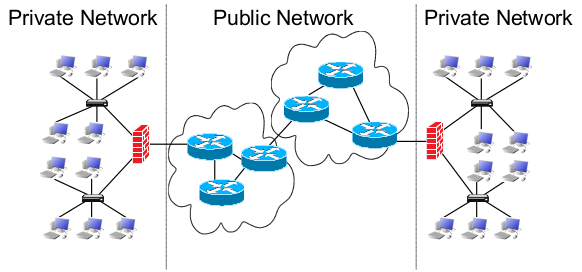
\includegraphics[width=\linewidth]{Assets/NetworkSecurity-Authentication-relation-in-inter-networks.png}

      %\begin{longtable}[]{@{}ll@{}}
      % \toprule
      % Authentication Relation & Application for securing\tabularnewline
      % \midrule
      % \endhead
      % Endsystem $\leftrightarrow$ Endsystem & User
      % Channels\tabularnewline
      % Endsystem $\leftrightarrow$ Intermediate System &
      % Management Interfaces, Accounting\tabularnewline
      % Intermediate $\leftrightarrow$ Intermediate System &
      % Network Operation: Signaling, Routing, Accounting, ...\tabularnewline
      % \bottomrule
      %\end{longtable}

      \subsection{Schlussfolgerung}
      \begin{itemize*}
            \item Die Integration von Sicherheitsdiensten in Kommunikationsarchitekturen wird von zwei Hauptfragen geleitet:
            \begin{itemize*}
                  \item Welcher Sicherheitsdienst in welchem Knoten?
                  \item Welcher Sicherheitsdienst in welcher Schicht?
            \end{itemize*}
            \item Diese Design-Entscheidungen können auch durch einen Blick auf ein pragmatisches Modell der vernetzten Datenverarbeitung geleitet werden, das vier verschiedene Ebenen unterscheidet, auf denen Sicherheitsdienste realisiert werden können:
            \begin{itemize*}
                  \item Anwendungs-/Endsystem-/Subnetz-/Link-Ebene
            \end{itemize*}
            \item Da es verschiedene Gründe für und gegen jede Option gibt, gibt es keine einheitliche Lösung für dieses Designproblem.
            \item In diesem Kurs werden wir daher einige Beispiele für die Integration von Sicherheitsdiensten in Netzarchitekturen untersuchen, um die Auswirkungen der getroffenen Designentscheidungen besser zu verstehen
      \end{itemize*}

      \section{Sicherheitsprotokolle der Datenübertragungsschicht}
      \begin{itemize*}
            \item IEEE 802.1Q, IEEE 802.1X \& IEEE 802.1AE
            \item Point-to-Point Protocol (PPP)
            \item Point-to-Point Tunneling Protocol (PPTP)
            \item Layer 2 Tunneling Protocol (L2TP)
            \item Virtual Private Networks (VPN)
      \end{itemize*}

      \subsection{Anwendungsbereich von Sicherheitsprotokollen der Verbindungsschicht}
      \begin{itemize*}
            \item Nach dem klassischen Verständnis des OSI-Modells stellt die Verbindungsschicht einen gesicherten Datenübertragungsdienst zwischen zwei gleichrangigen Einheiten bereit, die direkt über ein Kommunikationsmedium miteinander verbunden sind.
            \item Ihre Hauptaufgaben sind:
            \begin{itemize*}
                  \item Fehlererkennung und -korrektur
                  \item Medium Access Control (MAC, nicht zu verwechseln mit Message Authentication Code) für gemeinsam genutzte Medien, z.B. Ethernet usw.
            \end{itemize*}
            \item Nicht alle heutigen Netzwerktechnologien passen in dieses Modell:
            \begin{itemize*}
                  \item Einwahlverbindungen zu einem Internetdienstanbieter
                  \item Lösungen für virtuelle private Netzwerke (VPN)
            \end{itemize*}
            \item In diesem Kurs geben wir uns mit der folgenden Definition zufrieden:
            \begin{itemize*}
                  \item Der Zweck eines Link-Layer-Sicherheitsprotokolls besteht darin, bestimmte Sicherheitseigenschaften der Link-Layer-PDUs zu gewährleisten, d. h. der PDUs der Protokollschicht, die die PDUs der Netzwerkschicht (z.B. IP) tragen.
            \end{itemize*}
      \end{itemize*}

      \subsection{IEEE 802.1}
      \subsubsection{Die IEEE 802.1 Standardfamilie: Hintergrund und Ziele}
      \begin{itemize*}
            \item Das Institute of Electrical and Electronics Engineers (IEEE) 802 LAN/MAN Standards Committee entwickelt Standards für lokale Netzwerke und Metropolitan Area Networks.
            \item Die am weitesten verbreiteten Standards sind:
            \begin{itemize*}
                  \item Ethernet-Familie (802.3, allgemein als CSMA/CD bezeichnet),
                  \item Drahtloses LAN (802.11)
                  \item WIMAX (802.16)
            \end{itemize*}
            \item Die IEEE 802.1-Standards:
            \begin{itemize*}
                  \item Können mit verschiedenen IEEE 802.x Technologien verwendet werden
                  \item Definieren unter anderem verschiedene explizite Sicherheitsdienste oder Dienste, die zur Erreichung von Sicherheitszielen verwendet werden können
            \end{itemize*}
      \end{itemize*}

      \subsubsection{IEEE 802.1Q}
      Ziele und Dienste. Der Standard IEEE 802.1Q
      \begin{itemize*}
            \item Ermöglicht die Schaffung von ,,miteinander verbundenen IEEE-802-Standard-LANs mit unterschiedlichen oder identischen Methoden der Medienzugriffskontrolle'', d. h. die Schaffung separater virtueller lokaler Netzwerke (VLANs) über eine physische Infrastruktur
            \item Obwohl es sich nicht um einen echten Sicherheitsstandard handelt, wird er häufig verwendet, um verschiedene Benutzer und Dienste voneinander zu trennen, z.B. nicht vertrauenswürdige Gastcomputer von Unternehmensservern, ohne eine neue Infrastruktur einzurichten
            \item Wird verwendet, um Zugangskontrolle auf Verbindungsebene zu realisieren
      \end{itemize*}

      Grundlegende Funktionsweise
      \begin{itemize*}
            \item Jedes Netzwerkpaket wird mit einem VLAN-Tag versehen, der eine 12-Bit-VLAN-ID enthält, die ein virtuelles Netzwerk identifiziert
            \item Switches stellen sicher, dass Pakete mit bestimmten VLAN-IDs nur an bestimmte Netzwerk-Ports zugestellt werden, z.B. wird ein VLAN mit internen Firmeninformationen nicht an einen öffentlich zugänglichen Port zugestellt
            \item Die VLAN-ID ist nicht kryptografisch geschützt!
            \begin{itemize*}
                  \item VLAN IDs müssen auf andere Weise, d.h. physikalisch, gesichert werden!
                  \item Normalerweise werden VLAN-IDs am ersten vertrauenswürdigen Switch eingefügt und am letzten vertrauenswürdigen Switch auf dem Weg durch das Netzwerk entfernt
            \end{itemize*}
      \end{itemize*}

      Typisches Einführungsszenario
      \begin{itemize*}
            \item Normalerweise wird das vertrauenswürdige innere Netzwerk durch physische Mittel geschützt
            \item Verschiedene Ports zum vertrauenswürdigen Kern werden VLANs zugeordnet
            \item VLANs sind virtuell verbunden, dürfen aber nicht auf andere VLANs zugreifen
            \item VLANs werden normalerweise gekoppelt durch
            \begin{itemize*}
                  \item Router, die mehrere Schnittstellen in den verschiedenen VLANs haben
                  \item Router, die selbst zum vertrauenswürdigen Netzwerk gehören und selbst getaggte Frames empfangen und senden können (kann gefährlich sein, Wechselwirkung zwischen Routing und VLANs)
            \end{itemize*}
            %\item 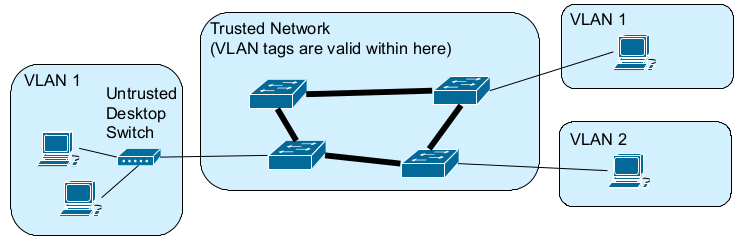
\includegraphics[width=\linewidth]{Assets/NetworkSecurity-ieee802.1q-scenario.png}
      \end{itemize*}

      Weitere Diskussion
      \begin{itemize*}
            \item 802.1Q ermöglicht eine einfache Trennung verschiedener Sicherheitsdomänen innerhalb eines vertrauenswürdigen Netzwerks
            \begin{itemize*}
                  \item Ermöglicht auch die Priorisierung bestimmter VLANs (z.B. um die Verwaltung von Geräten zu ermöglichen, wenn der Rest des Netzes von einem Angreifer überflutet wird)
                  \item VLAN-Tags können gestapelt werden, z.B. um verschiedene Kunden zu trennen, die eigene VLANs einrichten
            \end{itemize*}
            \item Diskussion über die Sicherheit:
            \begin{itemize*}
                  \item Die Sicherheit hängt davon ab, dass kein einziges Gerät in der vertrauenswürdigen Domäne kompromittiert wird!
                  \item Alle Switches müssen korrekt konfiguriert sein, d.h. kein einziger Switch darf eingehenden Verkehr aus einem nicht vertrauenswürdigen Netz zulassen, der bereits getaggt ist
                  \item Paketfluten in einem VLAN können sich auch auf andere VLANs auswirken
                  \item Router, die an mehreren VLANs teilnehmen, können auf einer Schnittstelle Pakete aus verschiedenen VLANs empfangen, aber
                  \item Anstatt ein striktes Routing zu einer anderen Schnittstelle (z.B. dem Internet) durchzuführen, könnte ein Angreifer diesen Router nutzen, um über dieselbe Schnittstelle zurück in ein anderes VLAN zu routen (sogenannter Layer-2-Proxy-Angriff)
                  \item Kann sogar funktionieren, wenn VLAN 1 und VLAN 2 das gleiche IP-Subnetz nutzen!
            \end{itemize*}
      \end{itemize*}

      \subsubsection{IEEE 802.1X}
      \begin{itemize*}
            \item Ziel ist es, ,,den Zugang zu den von einem LAN angebotenen Diensten auf diejenigen Benutzer und Geräte zu beschränken, die diese Dienste nutzen dürfen''
            \item Definiert eine portbasierte Netzwerkzugriffskontrolle, um ein Mittel zur ,,Authentifizierung und Autorisierung von Geräten bereitzustellen, die an einen LAN-Port mit Punkt-zu-Punkt-Verbindungseigenschaften angeschlossen sind''.
      \end{itemize*}

      Kontrollierte und unkontrollierte Ports
      \begin{itemize*}
            \item IEEE 802.1X führt den Begriff der zwei logischen Ports ein:
            \item Der unkontrollierte Port ermöglicht die Authentifizierung eines Geräts
            \item Der kontrollierte Port ermöglicht es einem authentifizierten Gerät, auf LAN-Dienste zuzugreifen
            %\item 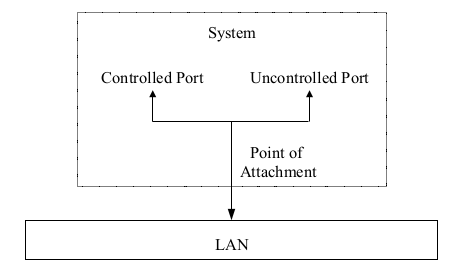
\includegraphics[width=\linewidth]{Assets/NetworkSecurity-ieee802.1X-ports.png}
      \end{itemize*}

      Rollen
      \begin{itemize*}
            \item Es werden drei Hauptrollen unterschieden:
            \begin{itemize*}
                  \item Ein Gerät, das den von einem IEEE 802.1X LAN angebotenen Dienst nutzen möchte, agiert als Supplicant, der den Zugriff auf den kontrollierten Port anfordert
                  \item Der Anschlusspunkt an die LAN-Infrastruktur (z.B. eine MAC-Brücke) fungiert als Authentifikator, der den Supplicant auffordert, sich zu authentifizieren.
                  \item Der Authentifikator prüft die vom Antragsteller vorgelegten Anmeldeinformationen nicht selbst, sondern leitet sie zur Überprüfung an seinen Authentifizierungsserver weiter.
            \end{itemize*}
            \item Zugriff auf ein LAN mit IEEE 802.1X Sicherheitsmaßnahmen:
            \begin{itemize*}
                  \item Vor einer erfolgreichen Authentifizierung kann der Antragsteller auf den unkontrollierten Port zugreifen:
                  \item Der Port ist unkontrolliert in dem Sinne, dass er den Zugriff vor der Authentifizierung erlaubt.
                  \item Dieser Port erlaubt jedoch nur einen eingeschränkten Zugriff
                  \item Die Authentifizierung kann durch den Supplicant oder den Authenticator initiiert werden.
                  \item Nach erfolgreicher Authentifizierung wird der kontrollierte Port geöffnet.
            \end{itemize*}
      \end{itemize*}

      Sicherheitsprotokolle und Nachrichtenaustausch
      \begin{itemize*}
            \item IEEE 802.1X definiert keine eigenen Sicherheitsprotokolle, sondern befürwortet die Verwendung bestehender Protokolle:
            \begin{itemize*}
                  \item Das Extensible Authentication Protocol (EAP) kann eine grundlegende Geräteauthentifizierung realisieren
                  \item Wenn die Aushandlung eines Sitzungsschlüssels während der Authentifizierung erforderlich ist, wird die Verwendung des EAP TLS Authentication Protocol empfohlen
                  \item Außerdem wird empfohlen, den Authentifizierungsserver mit dem Remote Authentication Dial In User Service (RADIUS) zu realisieren.
            \end{itemize*}
            \item Der Austausch von EAP Nachrichten zwischen Supplicant und Authenticator wird mit dem EAP over LANs (EAPOL) Protokoll realisiert:
            \begin{itemize*}
                  \item EAPOL definiert die Verkapselungstechniken, die verwendet werden sollen, um EAP-Pakete zwischen Supplicant Port Access Entities (PAE) und Authenticator PAEs in einer LAN-Umgebung zu übertragen.
                  \item EAPOL-Rahmenformate wurden für verschiedene Mitglieder der 802.x-Protokollfamilie definiert, z.B. EAPOL für Ethernet, ...
                  \item Zwischen Supplicant und Authenticator können RADIUS-Nachrichten verwendet werden
            \end{itemize*}
      \end{itemize*}

      Beispiel für eine 802.1X-Authentifizierung''(Assets/NetworkSecurity-ieee802.1X-example.png)
      \subsubsection{IEEE 802.1AE}
      Ziele
      \begin{itemize*}
            \item Der Standard IEEE 802.1AE wird auch als MAC-Sicherheit (MACsec) bezeichnet
            \item Ermöglicht autorisierten Systemen, die sich an LANs in einem Netzwerk anschließen und diese miteinander verbinden, die Vertraulichkeit der übertragenen Daten zu wahren und Maßnahmen gegen Frames zu ergreifen, die von nicht autorisierten Geräten übertragen oder verändert werden. ''
            \item Schützt Pakete durch kryptografische Mittel zwischen Geräten, z.B. zwischen Switches oder einem Computer und einem Switch
            \item Setzt eine gültige Authentifizierung voraus und ist somit eine Erweiterung von 802.1X
            \item Kryptografische Schlüssel werden auch während der 802.1X-Authentifizierungsphase abgeleitet
            \item Kann Datenursprungsauthentifizierung und optional Vertraulichkeit durchführen
            \item Unterstützt AES-128 und AES-256 in GCM, wobei die Unterstützung von AES-128-GCM obligatorisch ist!
      \end{itemize*}

      Frame-Format
      \begin{itemize*}
            %\item 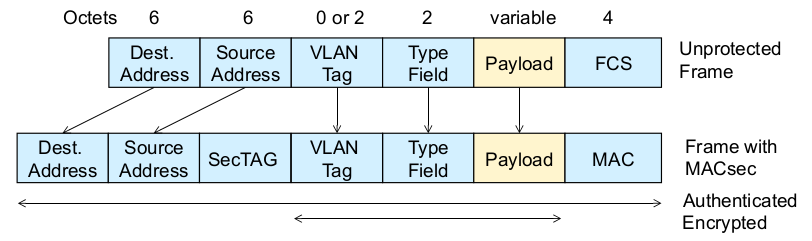
\includegraphics[width=\linewidth]{Assets/NetworkSecurity-ieee802.1AE-frame.png}
            \item Quell- und Zieladressen werden im Klartext gesendet
            \item VLAN-Tag, Typfeld und Nutzdaten werden ebenfalls verschlüsselt
            \item Ein neuer 8-16 Byte langer SecTAG wird eingefügt
            \begin{itemize*}
                  \item Beginnt mit 0x88e5, um ein Protokoll für ältere Geräte zu emulieren
                  \item Enthält einen 4-Byte-Paketzähler (wird als IV verwendet, auch um Replay-Angriffe abzuwehren)
            \end{itemize*}
            \item FCS wird durch einen kryptografischen MAC von 8-16 Byte ersetzt und von MACsec berechnet, optional kann ein zusätzlicher CRC-FCS für ältere Geräte hinzugefügt werden
      \end{itemize*}

      Diskussion über Sicherheit
      \begin{itemize*}
            \item MACsec erlaubt es, Verbindungen zu sichern, z.B. zwischen Gebäuden auf einem Campus
            \item Es bietet keinen Schutz gegen kompromittierte Geräte!
            \item Wenn es in Kombination mit 802.1Q verwendet wird, kann die vertrauenswürdige Computerbasis immer noch ziemlich groß sein...
            \item Die Verwendung des GCM unterliegt den in Kapitel 5 beschriebenen potenziellen Problemen
            \item Derzeit unterstützen nur hochwertige Switches MACsec
      \end{itemize*}

      \subsection{Punkt-zu-Punkt-Protokoll}
      Zweck und Aufgaben
      \begin{itemize*}
            \item Große Teile des Internets beruhen auf Punkt-zu-Punkt-Verbindungen:
            \begin{itemize*}
                  \item Wide Area Network (WAN)-Verbindungen zwischen Routern
                  \item Einwahlverbindungen von Hosts über Modems und Telefonleitungen
            \end{itemize*}
            \item Protokolle für diesen Zweck:
            \begin{itemize*}
                  \item Serial Line IP (SLIP): keine Fehlererkennung, unterstützt nur IP, keine dynamische Adressvergabe, keine Authentifizierung
                  \item Point-to-Point Protocol (PPP): Nachfolger von SLIP, unterstützt IP, IPX, ...
                  % \item 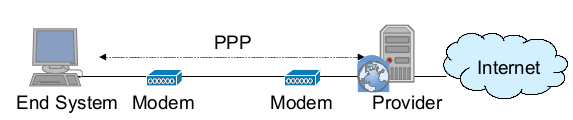
\includegraphics[width=\linewidth]{Assets/NetworkSecurity-Point-to-Point.png}
            \end{itemize*}
            \item PPP ,,RFC 1661/1662''
            \begin{itemize*}
                  \item Schicht-2-Rahmenformat mit Rahmenbegrenzung und Fehlererkennung
                  \item Kontrollprotokoll (Link Control Protocol, LCP) für Verbindungsaufbau, -test, -aushandlung und -abbau
                  \item Separate Netzwerkkontrollprotokolle (NCP) für unterstützte Schicht-3-Protokolle
            \end{itemize*}
      \end{itemize*}

      Packet Format
      \begin{itemize*}
            \item Zeichenorientierte (statt bitorientierte) $\Rightarrow$ byteausgerichtete Rahmen
            \item Code-Transparenz wird durch Zeichenstuffing erreicht
            \item Normalerweise werden nur unnummerierte Frames übertragen, in Szenarien mit hoher Fehlerwahrscheinlichkeit (drahtlose Kommunikation) kann jedoch ein zuverlässigerer Modus mit Sequenznummern und erneuten Übertragungen ausgehandelt werden
            \item Unterstützte Protokolle für das Nutzdatenfeld sind u.a.: IP, IPX, Appletalk
            \item Wenn nicht anders ausgehandelt, beträgt die maximale Nutzdatengröße 1500 Byte.
            \item Zusätzliche Aushandlung unterstützt kleinere Paketköpfe
            %\item \includegraphics[width=\linewidth]{Assets/NetworkSecurity-Punkt-zu-Punkt-Format.png}
      \end{itemize*}

      Eine typische PPP-Verbindung
      \begin{itemize*}
            \item Nutzungsszenario ,,Internetzugang eines PCs über Modem''
            \begin{itemize*}
                  \item Der Benutzer ruft den Internet Service Provider (ISP) über ein Modem an und stellt eine ,,physikalische'' Verbindung über den ,,Plain Old Telephone Service'' (POTS) her.
                  \item Anrufer sendet mehrere LCP-Pakete in PPP-Frames, um die gewünschten PPP-Parameter auszuwählen
                  \item Sicherheitsspezifische Aushandlung (siehe unten)
                  \item Austausch von NCP-Paketen zur Konfiguration der Netzwerkschicht: z.B. Konfiguration von IP einschließlich dynamischer Zuweisung einer IP-Adresse über Dynamic Host Configuration Protocol (DHCP)
                  \item Der Anrufer kann wie jeder andere Host mit einer festen Verbindung zum Internet beliebige Internetdienste nutzen
                  \item Beim Verbindungsabbau werden die zugewiesene IP-Adresse und die Netzschichtverbindung freigegeben
                  \item Die Schicht-2-Verbindung wird über LCP freigegeben und das Modem baut die ,,physikalische'' Verbindung ab
            \end{itemize*}
      \end{itemize*}

      Link Control Protocol
      \begin{itemize*}
            \item Rahmenformat des Link Control Protocol (LCP):
            \begin{itemize*}
                  \item Code: configure-request, configure-ack, configure-nack, configure-reject, terminate-request, terminate-ack, code-reject, protocol-reject, echo-request, echo-reply, discard-request
                  \item Länge: gibt die Länge des LCP-Pakets einschließlich des Codefelds usw. an
                  \item Daten: null oder mehr Oktette befehlsspezifischer Daten
                  % \item 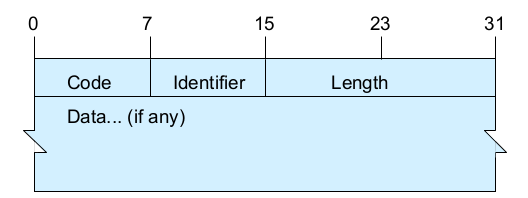
\includegraphics[width=\linewidth]{Assets/NetworkSecurity-Point-to-Point-LCP.png}
            \end{itemize*}
            \item Die Konfigurationsprimitive von LCP ermöglichen die Konfiguration der
            Verbindungsschicht:
            \begin{itemize*}
                  \item Es gibt verschiedene Optionen für dieses Primitiv zur Konfiguration verschiedener Aspekte (max. Empfangseinheit, Protokollkompression, Authentifizierung, ...)
            \end{itemize*}
      \end{itemize*}

      Sicherheitsdienste
      \begin{itemize*}
            \item Die ursprüngliche Version von PPP ,,RFC 1661'' schlägt die optionale Ausführung eines Authentifizierungsprotokolls nach der Verbindungsaufbauphase vor:
            \begin{itemize*}
                  \item Falls erforderlich, wird die Authentifizierung von einer Peer-Entität über einen LCP Configuration-Request am Ende der Verbindungsaufbauphase gefordert
                  \item Ursprünglich sind zwei Authentifizierungsprotokolle definiert worden:
                  \begin{itemize*}
                        \item Passwort-Authentifizierungsprotokoll (PAP)
                        \item Challenge-Handshake-Authentifizierungsprotokoll (CHAP)
                  \end{itemize*}
                  \item Inzwischen ist ein erweiterbares Protokoll definiert worden:
                  \begin{itemize*}
                        \item Erweiterbares Authentifizierungsprotokoll (EAP)
                        \item PPP EAP Transport Level Security Protocol (PPP-EAP-TLS)
                  \end{itemize*}
            \end{itemize*}
            \item Außerdem kann nach der Authentifizierung eine Verschlüsselung ausgehandelt werden:
            \begin{itemize*}
                  \item Protokolle:
                  \begin{itemize*}
                        \item Encryption Control Protocol (ECP) zur Aushandlung
                        \item PPP DES-Verschlüsselungsprotokoll (DESE)
                        \item PPP-Dreifach-DES-Verschlüsselungsprotokoll (3DESE)
                  \end{itemize*}
            \end{itemize*}
      \end{itemize*}

      Authentifizierungsprotokolle
      \begin{itemize*}
            \item Passwort-Authentifizierungs-Protokoll (PAP)
            \begin{itemize*}
                  \item PAP wurde 1992 in RFC 1334 definiert.
                  \item Das Protokoll ist sehr einfach
                  \begin{itemize*}
                        \item Voraussetzung: der Authentifikator kennt das Passwort der Peer-Entität
                        \item Am Ende der Verbindungsaufbauphase fordert eine Entität, Authenticator genannt, die Peer-Entität auf, sich mit PAP zu authentifizieren
                        \item Die Peer-Entität sendet eine Authenticate-Request-Nachricht mit ihrer Peer-ID und ihrem Passwort
                        \item Der Authentifikator prüft, ob die bereitgestellten Informationen korrekt sind und antwortet entweder mit einem Authenticate-ack oder einem Authenticate-nack
                  \end{itemize*}
                  \item Da das Protokoll keinen kryptographischen Schutz bietet, ist es unsicher
                  \item PAP wird in den aktualisierten RFCs für die PPP-Authentifizierung nicht erwähnt
            \end{itemize*}
            \item Challenge Handshake Authentication Protocol (CHAP)
            \begin{itemize*}
                  \item CHAP ist ebenfalls in RFC 1334 und RFC 1994 definiert.
                  \item Es verwirklicht ein einfaches Challenge-Response-Protokoll
                  \begin{itemize*}
                        \item Voraussetzung: Authentifikator und Peer-Entität teilen ein Geheimnis
                        \item Nach der Verbindungsaufbauphase sendet der Authentifikator (A) eine Challenge-Nachricht, die einen Identifikator für diese Challenge, eine Zufallszahl $r_A$ und seinen Namen enthält, an die Peer-Entität (B): $A \rightarrow B: (1, Identifikator, r_A, A)$
                        \item Die Peer-Entität berechnet eine kryptografische Hash-Funktion über ihren Namen, das gemeinsame Geheimnis $K_{A,B}$ und die Zufallszahl $r_A$ und sendet die folgende Nachricht: $B \rightarrow A: (2, Kennung, H(B, K_{A,B}, r_A), B)$
                        \item Beim Empfang dieser Nachricht berechnet der Authentifikator den Hashwert neu und vergleicht ihn mit dem empfangenen Wert; wenn beide Werte übereinstimmen, antwortet er mit einer Erfolgsmeldung
                        \item RFC 1994 legt fest, dass MD5 als Hash-Funktion unterstützt werden muss, aber die Verwendung anderer Hash-Funktionen kann ausgehandelt werden
                  \end{itemize*}
            \end{itemize*}
            \item CHAP-Nachrichtenformat:
            \begin{itemize*}
                  \item Code: 1 \textasciitilde{} Herausforderung / 2 \textasciitilde{} Antwort / 3 \textasciitilde{} Erfolg / 4 \textasciitilde{} Fehler
                  \item Identifier: ein Oktett, das bei jeder gesendeten Challenge geändert werden muss
                  \item Länge: die Gesamtlänge der CHAP-Nachricht in Oktetten
                  \item Value Size: ein Oktett, das die Länge des Wertes angibt
                  \item Wert: enthält die zufällige Herausforderung / die Antwort auf die Herausforderung
                  \item Name: ein oder mehrere Oktette, die das System identifizieren, das das Paket erstellt hat; die Größe des Namens wird anhand des Längenfeldes berechnet
                  % \item 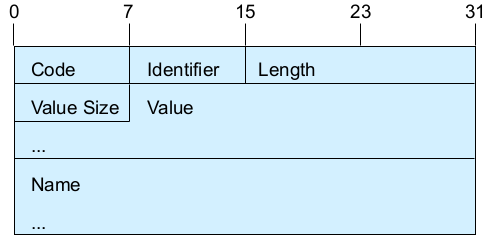
\includegraphics[width=\linewidth]{Assets/NetworkSecurity-Point-to-Point-CHAP1.png}
                  \item Nachricht:
                  \begin{itemize*}
                        \item Null oder mehr Oktette mit implementierungsabhängigem Inhalt
                        \item Der Inhalt soll für den Menschen lesbar sein und hat keinen Einfluss auf die Funktionsweise des Protokolls
                  \end{itemize*}
                  % \item 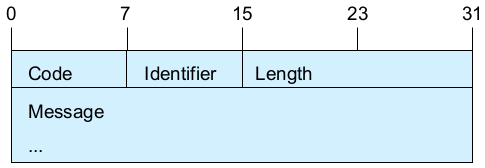
\includegraphics[width=\linewidth]{Assets/NetworkSecurity-Point-to-Point-CHAP2.png}
            \end{itemize*}
            \item Erweiterbares Authentifizierungsprotokoll (EAP)
            \begin{itemize*}
                  \item EAP ist ein allgemeines Protokoll für die PPP-Authentifizierung, das mehrere Authentifizierungsmethoden unterstützt
                  \item Die Hauptidee hinter EAP ist es, ein gemeinsames Protokoll bereitzustellen, um komplexere Authentifizierungsmethoden als ,,1 Frage + 1 Antwort'' durchzuführen.
                  \item Das Protokoll bietet grundlegende Primitive:
                  \begin{itemize*}
                        \item Anfrage, Antwort: weiter verfeinert durch Typfeld + typspezifische Daten
                        \item Success, Failure: zur Angabe des Ergebnisses eines Authentifizierungsaustauschs
                  \end{itemize*}
                  \item Typ-Felder
                  \begin{itemize*}
                        \item Identität
                        \item Benachrichtigung
                        \item Nak (nur Antwort, zur Beantwortung inakzeptabler Anfragetypen)
                        \item MD5 Challenge (dies entspricht CHAP)
                        \item One-Time Password (OTP)
                        \item Generische Token-Karte
                        \item EAP-TLS
                  \end{itemize*}
            \end{itemize*}
            \item Einmaliges Kennwort (One-Time Password, OTP)
            \begin{itemize*}
                  \item Die Grundidee von OTP besteht darin, ein ,,Passwort'' zu übermitteln, das nur für einen Durchlauf eines Authentifizierungsdialogs verwendet werden kann
                  \item Erstmalige Einrichtung:
                  \begin{itemize*}
                        \item Der Authentifikator A sendet einen Seed-Wert rA und die Peer-Entität B verkettet diesen mit seinem Passwort und berechnet einen Hash-Wert: $PW_N = H^N(r_A, password_B)$
                        \item Das Paar $(N, PW_N)$ wird ,,sicher'' an den Authentifikator übertragen und beim Authentifikator gespeichert.
                  \end{itemize*}
                  \item Dialog zur Authentifizierung:
                  \begin{itemize*}
                        \item $A\rightarrow B: N - 1$
                        \item $B\rightarrow A: PW_{N-1} := H^{N-1}(r_A, Passwort_B)$
                        \item A prüft, ob $H(PW_{N-1}) = PW_N$, und speichert $(N-1, PW_{N-1})$ als neue Authentifizierungsinformation für B
                  \end{itemize*}
                  \item Sicherheit: Um dieses Verfahren zu brechen, müsste ein Angreifer ein PWN abhören und $H^{-1}(PW_N)$ berechnen, was unpraktisch ist.
            \end{itemize*}
            \item Generische Token-Karte:
            \begin{itemize*}
                  \item Im Grunde ein Challenge-Response-Dialog
                  \item Eine Token-Karte wird verwendet, um eine Antwort auf eine Herausforderung zu berechnen:
                  \begin{itemize*}
                        \item Die Herausforderung wird dem Benutzer präsentiert, der sie in sein Token-Card-Gerät eintippen muss.
                        \item Die Token-Karte berechnet die Antwort und zeigt sie an.
                        \item Der Benutzer gibt die Antwort in das System ein, das sie als Antwort auf die Aufforderungsnachricht sendet.
                  \end{itemize*}
            \end{itemize*}
            \item PPP-EAP-TLS:
            \begin{itemize*}
                  \item TLS steht für Transport Layer Security
                  \item Es wird also der Authentifizierungsdialog von TLS ausgeführt
                  \item Dieser Dialog wird in Kapitel 12 über die Sicherheit der Transportschicht im Detail erläutert.
            \end{itemize*}
      \end{itemize*}

      Verschlüsselungsprotokolle
      \begin{itemize*}
            \item Nach dem Verbindungsaufbau und der Authentifizierungsphase kann die Verschlüsselung für eine PPP-Verbindung ausgehandelt werden
            \begin{itemize*}
                  \item Das Encryption Control Protocol (ECP) ist für die Konfiguration und Aktivierung von Datenverschlüsselungsalgorithmen an beiden Enden der PPP-Verbindung zuständig:
                  \begin{itemize*}
                        \item ECP verwendet das gleiche Rahmenformat wie LCP und führt zwei neue Primitive ein: Reset-Request und Reset-Ack zur Anzeige von Entschlüsselungsfehlern unabhängig für jede Richtung (nützlich für die kryptographische Resynchronisation)
                        \item Eine bestimmte Verschlüsselungsmethode wird mit dem configure-Primitiv ausgehandelt, das eine Option zur Angabe von DESE, 3DESE, Proprietär usw. enthält.
                        \item Proprietäre Verschlüsselungsprotokolle werden durch einen registrierten OUI (Organizational Unit Identifier) + einen herstellerspezifischen Wert identifiziert.
                        \item Genau ein ECP-Paket wird im PPP-Informationsfeld eines Link-Layer-Pakets transportiert
                        \item ECP-Pakete werden durch das PPP-Protokollfeld identifiziert
                        \begin{itemize*}
                              \item 0x8053 für ,,Standard'' Betrieb
                              \item 0x8055 für die Verschlüsselung einzelner Verbindungsdaten auf mehreren Verbindungen zum selben Ziel
                        \end{itemize*}
                  \end{itemize*}
            \end{itemize*}
            \item Das PPP DES Encryption Protocol (DESE)
            \begin{itemize*}
                  \item In diesem Kurs wird nur die aktualisierte Version DESEv2 behandelt
                  % \item 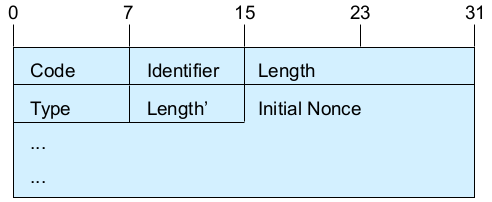
\includegraphics[width=\linewidth]{Assets/NetworkSecurity-Point-to-Point-DESE.png}
                  \item DESEv2 wird mit einer ECP-Konfigurationsanforderungsnachricht ausgehandelt:
                  \begin{itemize*}
                        \item Code: 1 \textasciitilde{} configure request
                        \item Identifier: ändert sich mit jeder neuen Anfrage
                        \item Länge: Gesamtlänge der Configure-Request-Nachricht
                        \item Type: 3 \textasciitilde{} DESEv2
                        \item Länge': 10 (die Länge dieser Konfigurationsoption)
                        \item Initial Nonce: ein Initialisierungsvektor für DES im CBC-Modus (8 Oktette)
                  \end{itemize*}
            \end{itemize*}
            \item PPP DESE v2 Nachrichtenformat
            \begin{itemize*}
                  \item Adresse: 0x11111111 (bei HDLC-ähnlichem Framing)
                  \item Steuerung: 0x00000011 (bei HDLC-ähnlicher Rahmung)
                  \item Protokoll-ID: 0x0053 \textasciitilde{} DESE (Standard) / 0x0055 \textasciitilde{} DESE (individuelle Verbindung)
                  \item Sequenznummer: anfänglich 0, diese Nummer wird von der verschlüsselnden Stelle bei jedem gesendeten Paket erhöht
                  \item Chiffriertext: die verschlüsselten Protokoll- und Informationsfelder eines PPP-Pakets
                  \begin{itemize*}
                        \item Nachrichten werden vor der Verschlüsselung auf ein Vielfaches von 8 Oktetten aufgefüllt
                        \item die Verschlüsselung erfolgt mit DES im CBC-Modus
                  \end{itemize*}
                  % \item 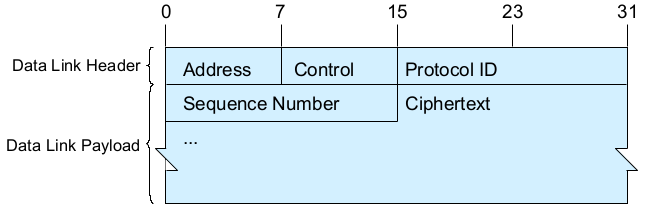
\includegraphics[width=\linewidth]{Assets/NetworkSecurity-Point-to-Point-DESE2.png}
            \end{itemize*}
            \item PPP 3DES Encryption Protocol (3DESE)
            \begin{itemize*}
                  \item PPP 3DESE ,,RFC2420'' ist dem PPP DESE sehr ähnlich
                  \item PPP 3DESE wird mit einer Configure-Request-Nachricht ausgehandelt, wobei das Type-Feld der Option auf 2 gesetzt ist (\textasciitilde{} 3DESE)
                  \item Die Verschlüsselung der PPP-Nutzdaten erfolgt wie bei DESE, mit dem Unterschied, dass 3DES mit 3 verschiedenen Schlüsseln verwendet wird
            \end{itemize*}
            \item Alle PPP-Verschlüsselungsprotokolle gehen davon aus, dass vor der
            Verschlüsselungsphase ein Sitzungsschlüssel für die
            Verschlüsselung/Entschlüsselung von PPP-Paketen vereinbart wurde
            \begin{itemize*}
                  \item Diese Annahme ist sinnvoll, da die Festlegung des Sitzungsschlüssels eine Aufgabe ist, die während der Authentifizierungsphase erfüllt werden sollte.
                  \item Allerdings unterstützt nur das PPP-EAP-TLS-Authentifizierungsprotokoll den Aufbau von Sitzungsschlüsseln.
            \end{itemize*}
      \end{itemize*}

      \subsubsection{Punkt-zu-Punkt-Tunneling-Protokoll (PPTP)}
      \begin{itemize*}
            \item PPP wurde ursprünglich für den Betrieb zwischen ,,direkt'' verbundenen Einheiten entwickelt, d.h. Einheiten, die eine gemeinsame Schicht-2-Verbindung haben
            \begin{itemize*}
                  \item Beispiel: ein PC und ein Einwahlrouter eines Internetanbieters, die über das Telefonnetz mittels Modem verbunden sind
            \end{itemize*}
            \item Die Grundidee von PPTP besteht darin, die Reichweite des Protokolls auf das gesamte Internet auszudehnen, indem der Transport von PPP-PDUs in IP-Paketen definiert wird
            \begin{itemize*}
                  \item Die Nutzlast von PPTP-PDUs sind also PPP-Pakete (ohne schicht-2-spezifische Felder wie HDLC-Flags, Bit-Einfügungen, Steuerzeichen, CRC-Fehlerprüfwerte usw.)
                  \item PPP-Pakete werden in GRE-Pakete (generische Routing-Kapselung) eingekapselt, die wiederum in IP-Pakete eingekapselt werden:
            \end{itemize*}
      \end{itemize*}

      %\begin{longtable}[]{@{}l@{}}
      % \toprule
      % \endhead
      % Media Header (e.g. Ethernet MAC header)\tabularnewline
      % IP Header\tabularnewline
      % GRE V.2 Header\tabularnewline
      % PPP Packet\tabularnewline
      % \bottomrule
      %\end{longtable}

      \subsubsection{PPTP: Freiwilliges vs. obligatorisches Tunneling}
      \begin{itemize*}
            \item PPTP realisiert einen ,,Tunnel'' über das Internet, der PPP-Pakete überträgt
            \item Ein solcher Tunnel kann zwischen verschiedenen Einheiten realisiert werden
            \item Einem Client-PC und einem PPTP Remote Access Server (RAS)
            \begin{itemize*}
                  \item Dies wird auch als freiwilliges Tunneling bezeichnet, da der Client-PC aktiv an der PPTP-Verarbeitung beteiligt ist.
                  \item Diese Variante ermöglicht die sichere Kommunikation zwischen einem Client-PC und einem bestimmten Subnetz unter Verwendung beliebiger Zugangs- und Zwischennetze
            \end{itemize*}
            \item Ein Point of Presence (POP) eines ISP und ein PPTP-Fernzugangsserver
            \begin{itemize*}
                  \item Dies wird auch als obligatorisches Tunneling bezeichnet, da der Client-PC nicht an der Entscheidung beteiligt ist, ob PPTP verwendet wird oder nicht.
                  \item Auf diese Weise lässt sich Sicherheit auf Subnetzebene realisieren, aber keine echte End-to-End-Sicherheit zwischen dem Client-PC und dem RAS
                  \item Beim obligatorischen Tunneling fungiert der ISP POP als Proxy-Client für den RAS
            \end{itemize*}
      \end{itemize*}

      %Obligatorische Tunneling-Protokollschichten
      %\begin{itemize*}
      %\item 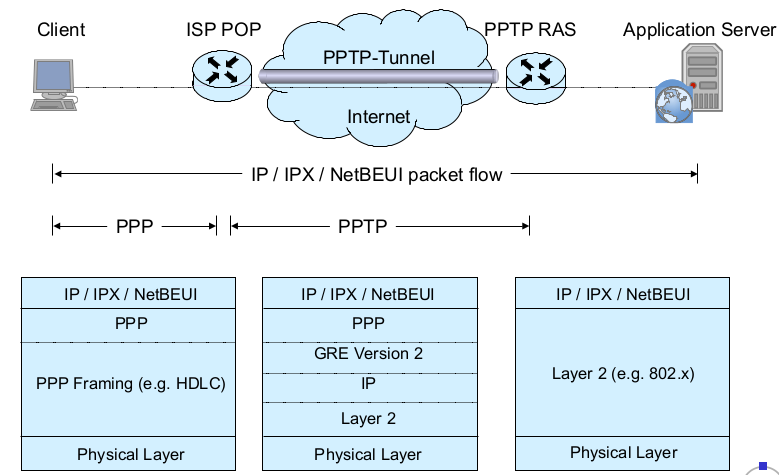
\includegraphics[width=\linewidth]{Assets/NetworkSecurity-PPTP-Tunneling-Protocol.png}
      %\item 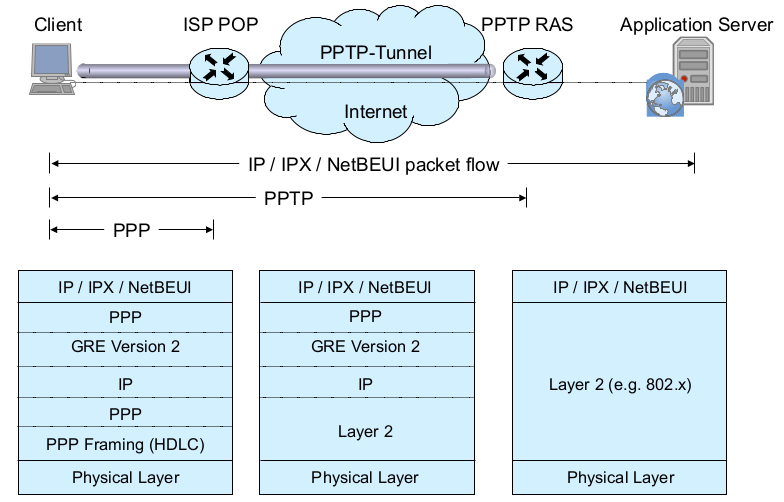
\includegraphics[width=\linewidth]{Assets/NetworkSecurity-PPTP-Tunneling-Protocol2.png}
      %\item 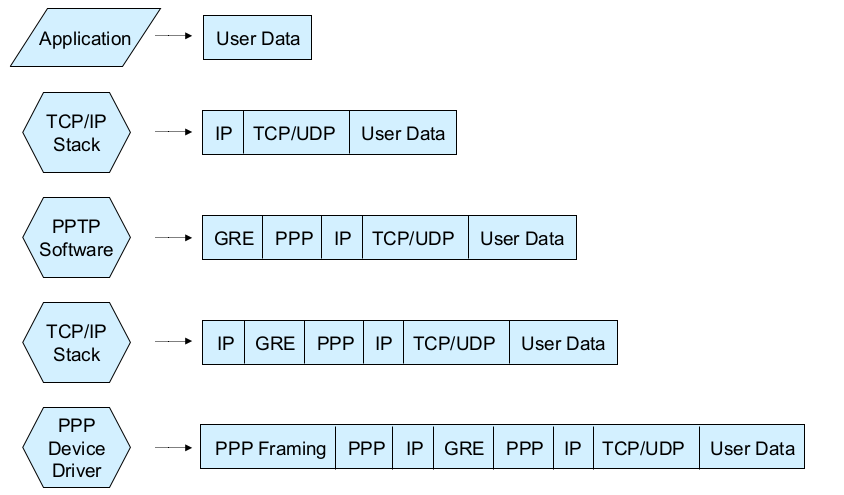
\includegraphics[width=\linewidth]{Assets/NetworkSecurity-PPTP-Packet-Construction-at-Client.png}
      %\end{itemize*}

      \subsubsection{PPTP / PPP Proprietäre Erweiterungen}
      \begin{itemize*}
            \item PPTP hat sich vor allem aufgrund der Unterstützung durch Microsoft durchgesetzt
            \begin{itemize*}
                  \item Es wurde unter aktiver Beteiligung von Microsoft entwickelt
                  \item Microsoft implementierte es als Teil seines Remote Access Service (RAS)
            \end{itemize*}
            \item Microsoft hat weitere ,,proprietäre'' Erweiterungen für PPP spezifiziert
            \begin{itemize*}
                  \item Microsoft PPP CHAP-Erweiterungen
                  \item Microsoft Point to Point Encryption Protocol
            \end{itemize*}
            \item Allerdings wurde eine Reihe von Schwachstellen in PPTP Version 1 und auch in einer verbesserten Version 2 entdeckt
            \begin{itemize*}
                  \item Ein allgemeiner Konsens, PPTP als Standardprotokoll zu übernehmen, konnte in den in den IETF-Arbeitsgruppen nicht erreicht werden.
                  \item Außerdem wurde ein ähnliches Protokoll (Layer 2 Forwarding, L2F) von Cisco als konkurrierender Ansatz vorgeschlagen
                  \item Infolgedessen wurde ein Kompromiss gefunden, der die Vorteile beider Vorschläge in einem einzigen Protokoll zusammenfasst: Layer 2 Tunneling Protocol (L2TP)
            \end{itemize*}
      \end{itemize*}

      \subsubsection{Vergleich von PPTP und L2TP}
      \begin{itemize*}
            \item Beide Protokolle
            \begin{itemize*}
                  \item verwenden PPP, um eine anfängliche Umhüllung für Benutzerpakete bereitzustellen
                  \item erweitern das PPP-Modell, indem sie erlauben, dass die Layer-2- und PPP-Endpunkte sich auf verschiedenen Geräten befinden
                  \item unterstützen freiwilliges und obligatorisches Tunneling
            \end{itemize*}
            \item Zugrundeliegendes Netzwerk
            \begin{itemize*}
                  \item PPTP benötigt ein IP-Netzwerk für den Transport seiner PDUs
                  \item L2TP unterstützt verschiedene Technologien: IP (unter Verwendung von UDP), permanente virtuelle Schaltungen (PVCs) von Frame Relay, virtuelle Schaltungen (VCs) von X.25 oder ATM VCs
            \end{itemize*}
            \item PPTP kann nur einen einzigen Tunnel zwischen Endpunkten unterstützen, L2TP ermöglicht die Verwendung mehrerer Tunnel zwischen Endpunkten
            \begin{itemize*}
                  \item L2TP ermöglicht z.B. die Erstellung verschiedener Tunnel für unterschiedliche Dienstqualitäten
            \end{itemize*}
            \item Beide Protokolle bieten eine Header-Kompression:  Mit Header-Kompression kommt L2TP mit 4 Byte Overhead aus, im Vergleich zu 6 Byte bei PPTP.
            \item L2TP ermöglicht eine Tunnelauthentifizierung, während PPTP dies nicht tut.
      \end{itemize*}

      \subsection{Virtuelle private Netzwerke}
      \begin{itemize*}
            \item Verschiedene Definitionen des Begriffs virtuelles privates Netzwerk (VPN):
            \begin{itemize*}
                  \item Ein privates Netz, das innerhalb einer öffentlichen Netzinfrastruktur, wie dem globalen Internet, aufgebaut ist.
                  \item Eine Kommunikationsumgebung, in der der Zugang kontrolliert wird, um Peer-Verbindungen nur innerhalb einer definierten Interessengemeinschaft zuzulassen, und die durch eine Form der Partitionierung eines gemeinsamen zugrundeliegenden Kommunikationsmediums aufgebaut ist, wobei dieses zugrundeliegende Kommunikationsmedium dem Netz Dienste auf nicht-exklusiver Basis bereitstellt
                  \item Ein logisches Computernetzwerk mit eingeschränkter Nutzung, das aus den Systemressourcen eines relativ öffentlichen, physischen Netzwerks (z.B. dem Internet) aufgebaut ist, oft unter Verwendung von Verschlüsselung und oft durch Tunneln von Verbindungen des virtuellen Netzwerks über das reale Netzwerk
                  \item Anmerkung: Die beiden letzteren Definitionen beinhalten explizit Sicherheitseigenschaften (kontrollierter Zugriff, Verschlüsselung), die erste hingegen nicht.
            \end{itemize*}
      \end{itemize*}

      \begin{quote}
            ,,Sicher, es ist viel billiger als eigene Frame-Relay-Verbindungen, aber es funktioniert ungefähr so gut, wie wenn man sich auf dem Times Square Watte in die Ohren steckt und so tut, als wäre sonst niemand da.'' (Wired Magazine Feb. 1998)
      \end{quote}

      Techniken zum Aufbau virtueller privater Netze
      \begin{itemize*}
            \item Nutzung dedizierter Verbindungen (Cut-Through-Mechanismen)
            \begin{itemize*}
                  \item Virtuelle Verbindungen über ATM oder Frame Relay
                  \item Multi-Protokoll über ATM (MPOA)
                  \item Multiprotokoll-Etiketten-Vermittlung (MPLS)
                  \item Sicherheitsdienste für Link Layer VPNs können effizient im Link Layer Protokoll realisiert werden; ein Beispiel ist die ATM Security Specification
            \end{itemize*}
            \item Kontrolliertes Routenleck / Routenfilterung
            \begin{itemize*}
                  \item Grundidee: Kontrolle der Routenausbreitung dahingehend, dass nur bestimmte Netze Routen für andere Netze erhalten
                  \item Damit soll ,,security by obscurity'' realisiert werden (also kein wirklicher Schutz!)
            \end{itemize*}
            \item Tunneln
            \begin{itemize*}
                  \item Generische Routing-Kapselung (GRE)
                  \item PPP / PPTP / L2TP
                  \item IPSec-Sicherheitsarchitektur für das Internet-Protokoll
            \end{itemize*}
      \end{itemize*}

      \section{Die IPsec-Architektur für das Internet-Protokoll}
      \subsection{Überblick}
      \begin{itemize*}
            \item Kurze Einführung in das Internet-Protokoll (IP)
            \item Sicherheitsprobleme von IP und Ziele von IPsec
            \item Die IPsec-Architektur
            \begin{itemize*}
                  \item Modi des IPsec-Sicherheitsprotokolls Transport/Tunnel-Modus
                  \item Alternativen zur Implementierung
                  \item IP-Sicherheitsrichtlinien-Datenbank (SPD)
                  \item Sicherheitsvereinigungen (SA) und die SA-Datenbank (SADB)
            \end{itemize*}
            \item IPsec Sicherheitsprotokolle
            \begin{itemize*}
                  \item Authentifizierungs-Header (AH)
                  \item Encapsulating Security Payload (ESP)
            \end{itemize*}
            \item Entitätsauthentifizierung und der Internet-Schlüsselaustausch (IKE)
      \end{itemize*}

      \subsection{Die TCP/IP-Protokollsuite}
      \begin{itemize*}
            \item IP (Internet Protocol): unzuverlässiges, verbindungsloses Netzwerkprotokoll
            \item TCP (Transmission Control Protocol): zuverlässiges, verbindungsorientiertes Transportprotokoll, realisiert über IP
            \item UDP (User Datagram Protocol): unzuverlässiges, verbindungsloses Transportprotokoll, bietet eine Anwendungsschnittstelle zu IP
            \item Beispiele für Anwendungsprotokolle
            \begin{itemize*}
                  \item HTTP: Hypertext-Übertragungsprotokoll
                  \item SMTP: Einfaches Mail-Übertragungsprotokoll
            \end{itemize*}
            %\item 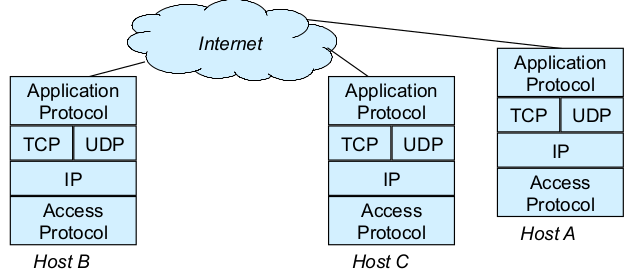
\includegraphics[width=\linewidth]{Assets/NetworkSecurity-tcp-ip-suite.png}
      \end{itemize*}

      \subsection{Das IPv4-Paketformat}
      \begin{itemize*}
            %\item 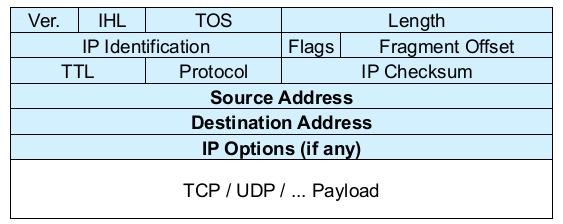
\includegraphics[width=\linewidth]{Assets/NetworkSecurity-ipv4-packet-format.png}
            \item Version (Ver.): 4 bit
            \begin{itemize*}
                  \item Derzeit ist Version 4 weit verbreitet
                  \item Version 6 ist bereits spezifiziert, aber es ist noch nicht klar, ob sie jemals zum Einsatz kommen wird
            \end{itemize*}
            \item IP-Header-Länge (IHL): 4 Bit
            \begin{itemize*}
                  \item Länge des IP-Headers in 32-Bit-Wörtern
            \end{itemize*}
            \item Art des Dienstes (TOS): 8 Bit
            \begin{itemize*}
                  \item Dieses Feld könnte verwendet werden, um die Verkehrsanforderungen eines Pakets anzugeben.
                  \item Jetzt: DCSP und Explicit Congestion (EC) Indication
            \end{itemize*}
            \item Länge: 16 Bit
            \begin{itemize*}
                  \item Die Länge des Pakets einschließlich des Headers in Oktetten
                  \item Dieses Feld ist, wie alle anderen Felder in der IP-Suite, in ,,big endian'' Darstellung
            \end{itemize*}
            \item Kennung: 16 Bit
            \begin{itemize*}
                  \item Dient der ,,eindeutigen'' Identifizierung eines IP-Datagramms
                  \item Wichtig für das Wiederzusammensetzen von fragmentierten IP-Datagrammen
            \end{itemize*}
            \item Flaggen: 3 Bit
            \begin{itemize*}
                  \item Bit 1: nicht fragmentieren
                  \item Bit 2: Datagramm fragmentiert
                  \item Bit 3: reserviert für zukünftige Verwendung
            \end{itemize*}
            \item Fragmentierungs-Offset: 13 Bit
            \begin{itemize*}
                  \item Die Position dieses Pakets im entsprechenden IP-Datagramm
            \end{itemize*}
            \item Lebenszeit (TTL): 8 Bit
            \begin{itemize*}
                  \item An jedem verarbeitenden Netzknoten wird dieses Feld um eins dekrementiert
                  \item Wenn die TTL 0 erreicht, wird das Paket verworfen, um Paketschleifen zu vermeiden.
            \end{itemize*}
            \item Protokoll: 8 Bit
            \begin{itemize*}
                  \item Gibt das (Transport-)Protokoll der Nutzlast an
                  \item Wird vom empfangenden Endsystem verwendet, um Pakete zwischen verschiedenen Transportprotokollen wie TCP, UDP, ... zu entmultiplexen.
            \end{itemize*}
            \item Prüfsumme: 16 Bit
            \begin{itemize*}
                  \item Schutz vor Übertragungsfehlern
                  \item Da es sich nicht um eine kryptografische Prüfsumme handelt, kann sie leicht gefälscht werden.
            \end{itemize*}
            \item Quelladresse: 32 Bit
            \begin{itemize*}
                  \item Die IP-Adresse des Absenders dieses Pakets
            \end{itemize*}
            \item Zieladresse: 32 Bit
            \begin{itemize*}
                  \item Die IP-Adresse des vorgesehenen Empfängers dieses Pakets
            \end{itemize*}
            \item IP-Optionen: variable Länge
            \begin{itemize*}
                  \item Ein IP-Header kann optional zusätzliche Informationen enthalten.
                  \item Da sie nicht Bestandteil von IPsec sind, werden sie in diesem Kurs nicht behandelt.
            \end{itemize*}
      \end{itemize*}

      \subsection{Sicherheitsprobleme des Internet-Protokolls}
      \begin{itemize*}
            \item Wenn eine Einheit ein IP-Paket empfängt, hat sie keine Garantie für
            \item Authentifizierung der Datenherkunft / Datenintegrität
            \begin{itemize*}
                  \item Das Paket wurde tatsächlich von der Einrichtung gesendet, auf die die Quelladresse des Pakets verweist.
                  \item Das Paket enthält den ursprünglichen Inhalt des Absenders, so dass es während des Transports nicht verändert worden ist.
                  \item Die empfangende Einrichtung ist tatsächlich die Einrichtung, an die der Absender das Paket senden wollte.
            \end{itemize*}
            \item Vertraulichkeit:
            \begin{itemize*}
                  \item Die ursprünglichen Daten wurden auf dem Weg vom Absender zum Empfänger nicht von Dritten eingesehen.
            \end{itemize*}
      \end{itemize*}

      \subsection{Sicherheitsziele von IPsec}
      \begin{itemize*}
            \item IPsec zielt darauf ab, die folgenden Sicherheitsziele zu gewährleisten:
            \begin{itemize*}
                  \item Authentifizierung der Datenherkunft / Verbindungslose Datenintegrität:
                  \begin{itemize*}
                        \item Es ist nicht möglich, ein IP-Datagramm mit einer maskierten IP-Quell- oder Zieladresse zu senden, ohne dass der Empfänger dies erkennen kann.
                        \item Es ist nicht möglich, ein IP-Datagramm während der Übertragung zu verändern, ohne dass der Empfänger diese Veränderung feststellen kann.
                        \item Wiedergabeschutz: Es ist nicht möglich, ein aufgezeichnetes IP-Paket zu einem späteren Zeitpunkt erneut abzuspielen, ohne dass der Empfänger dies erkennen kann.
                  \end{itemize*}
                  \item Vertraulichkeit:
                  \begin{itemize*}
                        \item Es ist nicht möglich, den Inhalt von IP-Datagrammen zu belauschen
                        \item Begrenzte Vertraulichkeit des Verkehrsflusses
                  \end{itemize*}
            \end{itemize*}
            \item Sicherheitspolitik:
            \begin{itemize*}
                  \item Sender, Empfänger und Zwischenknoten können den erforderlichen Schutz für ein IP-Paket gemäß einer lokalen Sicherheitsrichtlinie festlegen
                  \item Zwischenknoten und der Empfänger verwerfen IP-Pakete, die diese Anforderungen nicht erfüllen
            \end{itemize*}
      \end{itemize*}

      \subsection{Überblick über die IPsec-Standardisierung}
      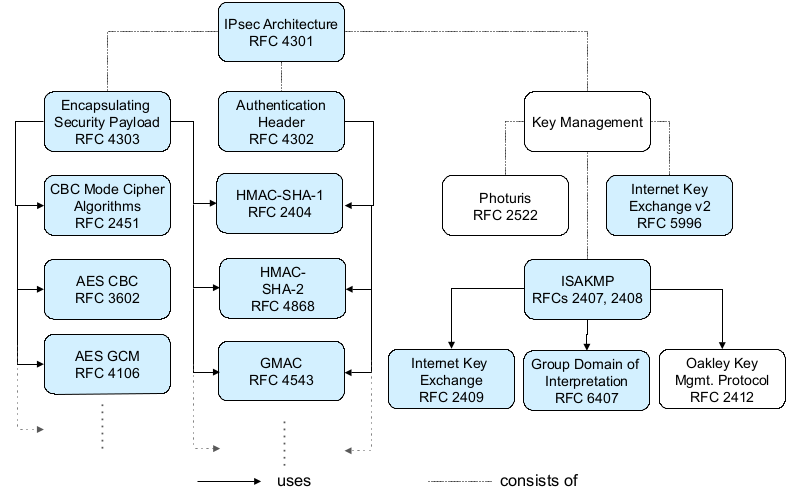
\includegraphics[width=\linewidth]{Assets/NetworkSecurity-IPsec-standardization.png}

      \subsection{Überblick über die IPsec-Architektur}
      \begin{itemize*}
            \item RFC 4301 definiert die grundlegende Architektur von IPsec:
            \begin{itemize*}
                  \item Konzepte:
                  \begin{itemize*}
                        \item Sicherheitsvereinigung (SA), Sicherheitsvereinigungsdatenbank (SADB)
                        \item Sicherheitsrichtlinien, Sicherheitsrichtlinien-Datenbank (SPD)
                  \end{itemize*}
                  \item Grundlegende IPsec-Protokolle:
                  \begin{itemize*}
                        \item Authentifizierungs-Header (AH)
                        \item Encapsulating Security Payload (ESP)
                  \end{itemize*}
                  \item Protokoll-Modi:
                  \begin{itemize*}
                        \item Transport-Modus
                        \item Tunnel-Modus
                  \end{itemize*}
                  \item Schlüsselmanagement-Verfahren:
                  \begin{itemize*}
                        \item IKE \& IKEv
                  \end{itemize*}
            \end{itemize*}
            \item RFC 4301 definiert die grundlegende Architektur von IPsec:
            \begin{itemize*}
                  \item Verwendung von verschiedenen kryptographischen Primitiven mit AH und ESP:
                  \begin{itemize*}
                        \item Verschlüsselung: 3DES-CBC, AES und andere CBC-Verschlüsselungsalgorithmen, AES-Zählermodus
                        \item Integrität: HMAC-MD5, HMAC-SHA-1, HMAC-SHA-2, HMAC- RIPEMD-160, AES-GMAC, AES-CMAC, AES-XCBC...
                        \item Authentifizierte Verschlüsselung: GCM und ,,Zähler mit CBC-MAC,, (CCM), beide für AES definiert
                  \end{itemize*}
            \end{itemize*}
            \item Eine Sicherheitsassoziation (SA) ist eine Simplex- ,,Verbindung'', die Sicherheitsdienste für den von ihr beförderten Verkehr bereitstellt.
            \begin{itemize*}
                  \item Sicherheitsdienste werden für eine SA entweder mit AH oder ESP bereitgestellt, jedoch nicht mit beiden.
                  \item Für bidirektionale Kommunikation sind zwei Sicherheitsverbindungen erforderlich.
                  \item Eine SA wird eindeutig durch ein Tripel identifiziert, das aus einem Sicherheitsparameterindex (SPI), einer IP-Zieladresse und einer Sicherheitsprotokollkennung (AH / ESP) besteht.
                  \item Eine SA kann zwischen den folgenden Gegenstellen eingerichtet werden:
                  \begin{itemize*}
                        \item Host $\leftrightarrow$ Host
                        \item Host $\leftrightarrow$ Gateway (oder andersherum)
                        \item Gateway $\leftrightarrow$ Gateway
                  \end{itemize*}
                  \item Es gibt zwei konzeptionelle Datenbanken, die mit SAs verbunden sind:
                  \begin{itemize*}
                        \item Die Sicherheitsrichtliniendatenbank (SPD) legt fest, welche Sicherheitsdienste für welche IP-Pakete auf welche Weise bereitgestellt werden sollen.
                        \item Die Sicherheitsassoziationsdatenbank (SADB)
                  \end{itemize*}
            \end{itemize*}
            \item Protokollmodi - Eine SA ist immer von einem der folgenden Typen:
            \begin{itemize*}
                  \item Der Transportmodus kann nur zwischen den Endpunkten einer Kommunikation verwendet werden:
                  \begin{itemize*}
                        \item host $\leftrightarrow$ host, oder
                        \item Host $\leftrightarrow$-Gateway, wenn das Gateway ein Kommunikationsendpunkt ist (z.B. für die Netzverwaltung)
                  \end{itemize*}
                  \item Der Tunnelmodus kann für beliebige Peers verwendet werden.
            \end{itemize*}
      \end{itemize*}

      Der Unterschied zwischen den beiden Modi ist, dass:

      Im Transportmodus wird lediglich ein sicherheitsspezifischer Header (+ eventueller Trailer) hinzugefügt
      \begin{itemize*} % \item 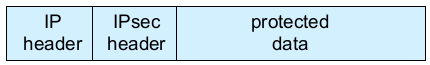
\includegraphics[width=\linewidth]{Assets/NetworkSecurity-ipsec-transport-mode.png} \end{itemize*}
            \item Der Tunnelmodus kapselt IP-Pakete ein: Die Verkapselung von IP-Paketen ermöglicht es einem Gateway, den Verkehr im Namen anderer Entitäten zu schützen (z.B. Hosts eines Subnetzes usw.)
            % \item 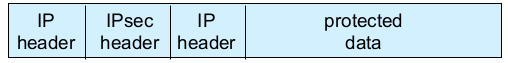
\includegraphics[width=\linewidth]{Assets/NetworkSecurity-ipsec-tunnel-mode.png} \end{itemize*}
            \item Der Authentifizierungs-Header (AH):
            \begin{itemize*}
                  \item Bietet Authentifizierung der Datenherkunft und Schutz vor Wiederholung
                  \item Wird als Header realisiert, der zwischen dem IP-Header und den zu schützenden Daten eingefügt wird
                  % \item 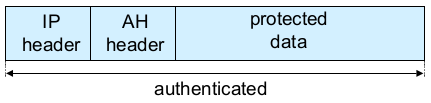
\includegraphics[width=\linewidth]{Assets/NetworkSecurity-ipsec-AH.png}
            \end{itemize*}
            \item Die einkapselnde Sicherheitsnutzlast (ESP):
            \begin{itemize*}
                  \item Bietet Authentifizierung der Datenherkunft, Vertraulichkeit und Schutz vor Wiederholung
                  \item Wird mit einem Header und einem Trailer realisiert, der die zu schützenden Daten einkapselt
                  % \item \includegraphics[width=\linewidth]{Assets/NetworkSecurity-ipsec-ESP.png}
            \end{itemize*}
            \item Die Einrichtung von Sicherheitsvereinigungen wird mit:
            \begin{itemize*}
                  \item Internet Security Association Key Management Protocol (ISAKMP):
                  \begin{itemize*}
                        \item Definiert einen generischen Rahmen für die Schlüsselauthentifizierung, den Schlüsselaustausch und die Aushandlung von Sicherheitsassoziationsparametern
                        \item Definiert kein spezifisches Authentifizierungsprotokoll, aber spezifiziert: Paketformate, Zeitgeber für die Weiterleitung, Anforderungen an den Nachrichtenaufbau
                  \end{itemize*}
                  \item Internet-Schlüsselaustausch (IKE):
                  \begin{itemize*}
                        \item Definiert ein Authentifizierungs- und Schlüsselaustauschprotokoll
                        \item Ist konform zu ISAKMP und kann für verschiedene Anwendungen verwendet werden
                        \item Der Aufbau von IPsec SAs zwischen zwei Entitäten wird in zwei Phasen realisiert:
                        \item Einrichtung einer IKE SA (definiert, wie man IPsec SAs einrichtet)
                        \item Einrichtung von IPsec SAs
                  \end{itemize*}
            \end{itemize*}
      \end{itemize*}

      \subsection{IPsec-Wiedergabeschutz (Replay protection)}
      \begin{itemize*}
            \item Sowohl AH- als auch ESP-geschützte IP-Pakete tragen eine
            Sequenznummer, die einen Wiedergabeschutz realisiert:
            \begin{itemize*}
                  \item Beim Einrichten einer SA wird diese Sequenznummer auf Null initialisiert.
                  \item Die Sequenznummer wird mit jedem gesendeten IP-Paket erhöht
                  \item Die Sequenznummer ist 32 Bit lang, es wird ein neuer Sitzungsschlüssel benötigt, bevor ein Wrap-around erfolgt
                  \item Der Empfänger eines IP-Pakets prüft, ob die Sequenznummer in einem Fenster zulässiger Nummern enthalten ist
                  % \item \includegraphics[width=\linewidth]{Assets/NetworkSecurity-ipsec-replay-protection.png} (Paket mit Sequenznummer N kann noch akzeptiert werden)
            \end{itemize*}
            \item Wenn ein empfangenes Paket eine Sequenznummer hat, die
            \begin{itemize*}
                  \item links vom aktuellen Fenster $\Rightarrow$ liegt, lehnt der Empfänger das Paket ab
                  \item innerhalb des aktuellen Fensters $\Rightarrow$ liegt, nimmt der Empfänger das Paket an
                  \item liegt rechts vom aktuellen Fenster $\Rightarrow$ der Empfänger nimmt das Paket an und schiebt das Fenster weiter
                  \item Natürlich werden IP-Pakete nur akzeptiert, wenn sie die Authentifizierungsprüfung bestehen und das Fenster wird niemals vor dieser Prüfung weitergeschaltet
            \end{itemize*}
            \item Die minimale Fenstergröße beträgt 32 Pakete (64 Pakete werden empfohlen)
            %\begin{itemize*}
            % \item \includegraphics[width=\linewidth]{Assets/NetworkSecurity-ipsec-replay-protection2.png}
            %\item Paket mit Sequenznummer N kann nicht mehr akzeptiert werden
            %\end{itemize*}
      \end{itemize*}

      \subsection{IPsec-Implementierungsalternativen: Host-Implementierung}
      \begin{itemize*}
            \item Vorteile der IPsec-Implementierung in Endsystemen:
            \begin{itemize*}
                  \item Bereitstellung von End-to-End-Sicherheitsdiensten
                  \item Bereitstellung von Sicherheitsdiensten auf einer Per-Flow-Basis
                  \item Fähigkeit, alle IPsec-Modi zu implementieren
            \end{itemize*}
            \item Zwei Hauptalternativen zur Integration:
      \end{itemize*}
      \begin{tabular}{p{4cm}|p{4cm}}
            Integriertes Betriebssystem & ,,Bump'' im Stack                                                                                         \\\hline
            Anwendung                   & Anwendung                                                                                                 \\
            Transport                   & Transport                                                                                                 \\
            Netzwerk + IPsec            & Netzwerk                                                                                                  \\
            IPsec                       &                                                                                                           \\
            Data Link                   & Data Link                                                                                                 \\
            Echte Betriebssystemintegration ist die Methode der Wahl, da sie die Duplizierung von Funktionalität
            vermeidet                   & Wenn das Betriebssystem nicht geändert werden kann, wird IPsec über den Datenverbindungstreiber eingefügt
      \end{tabular}

      \subsection{IPsec-Implementierungsalternativen: Router-Implementierung}
      \begin{itemize*}
            \item Vorteile der IPsec-Implementierung in Routern:
            \begin{itemize*}
                  \item Möglichkeit, IP-Pakete zu sichern, die zwischen zwei Netzen über ein öffentliches Netz wie das Internet fließen:
                  \begin{itemize*}
                        \item Ermöglicht die Einrichtung virtueller privater Netzwerke (VPNs)
                        \item Keine Notwendigkeit, IPsec in jedes Endsystem zu integrieren
                  \end{itemize*}
                  \item Fähigkeit zur Authentifizierung und Autorisierung des IP-Verkehrs, der von entfernten Benutzern eingeht
            \end{itemize*}
            \item Zwei Hauptalternativen für die Implementierung:
            % \item \includegraphics[width=\linewidth]{Assets/NetworkSecurity-ipsec-router-implementation.png}
      \end{itemize*}

      \subsection{Wann sollte welcher IPsec-Modus verwendet werden?}
      \begin{itemize*}
            \item In den meisten Fällen handelt es sich bei den Kommunikationsendpunkten um Hosts (Workstations, Server), aber das ist nicht unbedingt der Fall:
            \begin{itemize*}
                  \item Beispiel: ein Gateway wird über SNMP von einer Workstation verwaltet
            \end{itemize*}
            \item Der Transportmodus wird verwendet, wenn die ,,kryptografischen Endpunkte'' auch die ,,Kommunikationsendpunkte'' der gesicherten IP-Pakete sind
            \begin{itemize*}
                  \item Kryptografische Endpunkte: die Entitäten, die einen IPsec-Header (AH oder ESP) erzeugen/verarbeiten
                  \item Kommunikationsendpunkte: Quelle und Ziel eines IP-Pakets
                  % \item \includegraphics[width=\linewidth]{Assets/NetworkSecurity-communication-endpoints.png} 
            \end{itemize*}
            \item Der Tunnelmodus wird verwendet, wenn mindestens ein ,,kryptographischer Endpunkt'' nicht ein ,,Kommunikationsendpunkt'' der gesicherten IP-Pakete ist
            \begin{itemize*}
                  \item Dies ermöglicht Gateways, die den IP-Verkehr im Namen anderer Stellen sichern
                  % \item \includegraphics[width=\linewidth]{Assets/NetworkSecurity-communication-tunneling.png}
            \end{itemize*}
            \item Die obige Beschreibung der Anwendungsszenarien für den Tunnelmodus umfasst auch den Fall, dass nur ein kryptografischer Endpunkt kein Kommunikationsendpunkt ist:
            \begin{itemize*}
                  \item Beispiel: ein Sicherheitsgateway, das die Authentifizierung und/oder die Vertraulichkeit des IP-Verkehrs zwischen einem lokalen Teilnetz und einem über das Internet verbundenen Host sicherstellt (,,Road Warrior Szenario'')
                  % \item \includegraphics[width=\linewidth]{Assets/NetworkSecurity-communication-tunnelung-2.png}
            \end{itemize*}
      \end{itemize*}

      \subsection{Verschachtelung von Sicherheitsassoziationen}
      \begin{itemize*}
            \item Sicherheitsassoziationen können verschachtelt werden:
            \begin{itemize*}
                  \item Beispiel: Host A und Gateway RB führen eine Authentifizierung der Datenherkunft durch und die Gateways RA und RB führen eine Vertraulichkeit von Subnetz zu Subnetz durch
                  % \item \includegraphics[width=\linewidth]{Assets/NetworkSecurity-communication-nesting.png}
            \end{itemize*}
            \item Bei der Verschachtelung von SAs muss jedoch darauf geachtet werden, dass keine ,,falsche Klammerung'' von SAs erfolgt
            \begin{itemize*}
                  \item Ein Beispiel für eine gültige SA-Schachtelung:
                  % \item \includegraphics[width=\linewidth]{Assets/NetworkSecurity-communication-nesting-2.png} 
                  % \item \includegraphics[width=\linewidth]{Assets/NetworkSecurity-communication-nesting-3.png} 
                  \item Da das Paket von RB nach RD getunnelt wird, kann das Gateway RC den inneren IPsec-Header nicht verarbeiten
                  \item Ein mögliches Ergebnis dieser fehlerhaften Konfiguration könnte sein, dass das Paket zurück nach RC geroutet wird
            \end{itemize*}
      \end{itemize*}

      \subsection{Grundschema der IPsec-Verarbeitung: Ausgehende Pakete}
      \begin{itemize*}
            \item Nehmen wir an, die IP-Schicht eines Knotens (Host/Gateway) wird angewiesen, ein IP-Paket an einen anderen Knoten (Host/Gateway) zu senden
            \item Um IPsec zu unterstützen, muss sie die folgenden Schritte durchführen
            \item Feststellen, ob und wie das ausgehende Paket gesichert werden muss
            \begin{itemize*}
                  \item Dies wird durch einen Lookup im SPD realisiert
                  \item Wenn die Richtlinie ,,verwerfen'' vorschreibt, wird das Paket verworfen $\Rightarrow$ done
                  \item Wenn das Paket nicht gesichert werden muss, dann sende es $\Rightarrow$ done
            \end{itemize*}
            \item Ermitteln, welche SA auf das Paket angewendet werden soll
            \begin{itemize*}
                  \item Wenn es noch keine passende SA mit dem entsprechenden Knoten gibt, dann fordere den Key Management Demon auf, einen IKE durchzuführen
            \end{itemize*}
            \item Die ermittelte (und eventuell neu erstellte) SA in der SADB nachschlagen
            \item Führen Sie die von der SA festgelegte Sicherheitstransformation durch, indem Sie den Algorithmus, seine Parameter und den Schlüssel, wie in der SA angegeben, verwenden.
            \begin{itemize*}
                  \item Dies resultiert in der Konstruktion eines AH- oder ESP-Headers
                  \item Eventuell wird auch ein neuer (äußerer) IP-Header erstellt (Tunnelmodus)
            \end{itemize*}
            \item Senden Sie das resultierende IP-Paket $\Rightarrow$ done
      \end{itemize*}

      \subsection{Grundschema der IPsec-Verarbeitung: Eingehende Pakete}
      \begin{itemize*}
            \item Nehmen wir an, die IP-Schicht eines Knotens (Host/Gateway) empfängt ein IP-Paket von einem anderen Knoten (Host/Gateway)
            \item Um IPsec zu unterstützen, muss sie die folgenden Schritte durchführen
            \item Feststellen, ob das Paket einen IPsec-Header enthält, den diese Einheit verarbeiten soll:
            \begin{itemize*}
                  \item Wenn es einen solchen IPsec-Header gibt, dann suchen Sie die SA in der SADB, die durch den SPI des IPsec-Headers spezifiziert ist, und führen Sie die entsprechende IPsec-Verarbeitung durch
                  \item Wenn die SA, auf die der SPI verweist, (noch) nicht existiert, verwerfen Sie das Paket
            \end{itemize*}
            \item Ermitteln, ob und wie das Paket hätte geschützt werden sollen:
            \begin{itemize*}
                  \item Dies wird wiederum durch einen Lookup im SPD realisiert, wobei der Lookup im Falle von getunnelten Paketen durch Auswertung des inneren IP-Headers durchgeführt wird
                  \item Wenn die Richtlinie ,,Verwerfen'' vorschreibt, wird das Paket verworfen.
                  \item Wenn der Schutz des Pakets nicht mit der Richtlinie übereinstimmt, wird das Paket verworfen.
                  \item Wenn das Paket ordnungsgemäß gesichert wurde, dann übergebe es an die entsprechende Protokollinstanz (Netzwerk-/Transportschicht)
            \end{itemize*}
      \end{itemize*}

      \subsection{Auswahl der IPsec-Sicherheitspolitik}
      Die folgenden Selektoren, die aus den Headern der Netzwerk- und Transportschicht extrahiert werden, ermöglichen die Auswahl einer bestimmten Richtlinie im SPD:
      \begin{itemize*}
            \item IP-Quelladresse: Bestimmter Host, Netzwerkpräfix, Adressbereich oder Platzhalter
            \item IP-Zieladresse:
            \begin{itemize*}
                  \item Bestimmter Host, Netzwerk-Präfix, Adressbereich oder Platzhalter
                  \item Im Falle eingehender getunnelter Pakete wird der innere Header ausgewertet
            \end{itemize*}
            \item Protokoll:
            \begin{itemize*}
                  \item Der Protokoll-Identifikator des Transportprotokolls für dieses Paket
                  \item Dies ist möglicherweise nicht zugänglich, wenn ein Paket mit ESP gesichert ist.
            \end{itemize*}
            \item Ports der oberen Schicht: Falls zugänglich, die Ports der oberen Schicht für die sitzungsorientierte Policy-Auswahl
      \end{itemize*}

      \subsection{IPsec Security Policy Definition}
      \begin{itemize*}
            \item Policy Selectors werden verwendet, um spezifische Policy-Definitionen auszuwählen, spezifiziert
            \item Wie die Einrichtung einer IKE SA zwischen zwei Knoten durchgeführt werden soll
            \begin{itemize*}
                  \item Identifizierung: DNS-Name oder andere Namenstypen, wie in der IPsec-Domäne der Interpretation eines Protokolls zur Einrichtung von SAs definiert
                  \item Phase I-Modus: Hauptmodus oder aggressiver Modus (siehe unten)
                  \item Schutzsuite(n): Angabe, wie die IKE-Authentifizierung durchgeführt wird
            \end{itemize*}
            \item Welche und wie Sicherheitsdienste für IP-Pakete bereitgestellt werden sollen:
            \begin{itemize*}
                  \item Selektoren, die bestimmte Flüsse identifizieren
                  \item Sicherheitsattribute für jeden Fluss:
                  \item Sicherheitsprotokoll: AH oder ESP
                  \item Protokollmodus: Transport- oder Tunnelmodus
                  \item Sicherheitstransformationen: kryptografische Algorithmen und Parameter
                  \item Andere Parameter: SA-Lebensdauer, Replay-Fenster
                  \item Aktion: Verwerfen, Sichern, Umgehen
            \end{itemize*}
            \item Wenn bereits eine SA mit einem entsprechenden Sicherheitsendpunkt eingerichtet ist, wird im SPD auf diese verwiesen.
      \end{itemize*}

      \subsection{Die Encapsulating Security Payload}
      \begin{itemize*}
            \item ESP ist ein allgemeines Sicherheitsprotokoll, das IP-Paketen einen Wiederholungsschutz und einen oder beide der folgenden Sicherheitsdienste bietet:
            \begin{itemize*}
                  \item Vertraulichkeit durch Verschlüsselung der eingekapselten Pakete oder nur ihrer Nutzlast
                  \item Authentifizierung der Datenherkunft durch Erstellung und Hinzufügung von MACs zu Paketen
            \end{itemize*}
            \item Die ESP-Definition gliedert sich in zwei Teile:
            \begin{itemize*}
                  \item Die Definition des Basisprotokolls
                  \begin{itemize*}
                        \item Definition des Header- und Trailer-Formats
                        \item Verarbeitung des Basisprotokolls
                        \item Tunnel- und Transportmodusbetrieb
                  \end{itemize*}
                  \item Die Verwendung spezifischer kryptographischer Algorithmen mit ESP:
                  \begin{itemize*}
                        \item Verschlüsselung: 3DES-CBC, AES-CBC, AES-Zählmodus, Verwendung anderer Chiffren im CBC-Modus
                        \item Authentifizierung: HMAC-MD5-96, HMAC-SHA-96,...
                  \end{itemize*}
            \end{itemize*}
            %\item \includegraphics[width=\linewidth]{Assets/NetworkSecurity-ESP.png}
            \begin{itemize*}
                  \item Der ESP-Header folgt unmittelbar auf einen IP-Header oder einen AH-Header
                  \item Das Next-Header-Feld des vorangehenden Headers zeigt ,,50'' für ESP an
                  \item Das SPI-Feld gibt die SA an, die für dieses Paket verwendet werden soll:
                  \begin{itemize*}
                        \item Der SPI-Wert wird immer von der empfangenden Seite während der SA-Aushandlung bestimmt, da der Empfänger das Paket verarbeiten muss.
                  \end{itemize*}
                  \item Die Sequenznummer bietet, wie bereits erläutert, Schutz vor Wiederholung.
                  \item Wenn der verwendete kryptographische Algorithmus einen Initialisierungsvektor benötigt, wird dieser in jedem Paket am Anfang der Nutzlast im Klartext übertragen
                  \item Das Pad-Feld dient der Sicherstellung:
                  \begin{itemize*}
                        \item Auffüllen der Nutzlast bis zur erforderlichen Blocklänge der verwendeten Chiffre
                        \item Auffüllen der Nutzlast, um die Felder pad-length und next-header rechtsbündig in die höherwertigen 16 Bit eines 32-Bit-Wortes einzupassen
                  \end{itemize*}
                  \item Die Auffülllänge gibt die Anzahl der hinzugefügten Auffüllbytes an.
                  \item Das next-header-Feld des ESP-Headers gibt die eingekapselte Nutzlast an:
                  \begin{itemize*}
                        \item Im Falle des Tunnelmodus: IP
                        \item Im Falle des Transportmodus: ein beliebiges Protokoll der höheren Schicht wie TCP, UDP, ...
                  \end{itemize*}
                  \item Das optionale Feld authentication-data enthält eine MAC, falls vorhanden
            \end{itemize*}
            %\item \includegraphics[width=\linewidth]{Assets/NetworkSecurity-ESP-processing.png}
            %\item \includegraphics[width=\linewidth]{Assets/NetworkSecurity-ESP-prepare-header.png}
            %\item \includegraphics[width=\linewidth]{Assets/NetworkSecurity-ESP-inbound-processing.png}
            %\item \includegraphics[width=\linewidth]{Assets/NetworkSecurity-ESP-inbound-processing-2.png}
            \item Beachten Sie, dass das entkapselte IP-Paket ein fragmentiertes Paket sein kann:
            \begin{itemize*}
                  \item Dies kann vorkommen, wenn ESP von einem Router im Tunnelmodus angewendet wurde.
                  \item Um die Konformität mit der SA-Policy korrekt zu prüfen, müssen alle zu diesem Paket gehörenden Fragmente vom Router empfangen werden, bevor die Prüfung durchgeführt werden kann
                  \item Beispiel: In einer SA sind nur Pakete an einen bestimmten Port erlaubt
                  \item Die erforderliche Port-Information ist nur im ersten Fragment des IP-Pakets vorhanden
            \end{itemize*}
            \item Paketzustellung bedeutet Zustellung an die entsprechende Verarbeitungseinheit:
            \begin{itemize*}
                  \item Wenn ein anderer IPsec-Header für diese Entität vorhanden ist $\Rightarrow$ IPsec-Verarbeitung
                  \item Im Tunnelmodus $\Rightarrow$ Übermittlung des Pakets
                  \item Im Transportmodus $\Rightarrow$ Aufruf des entsprechenden Protokoll-Headers (TCP, UDP, etc.)
            \end{itemize*}
            \item Wenn ESP sowohl Vertraulichkeit als auch Authentifizierung bietet, können für beide Dienste unterschiedliche Schlüssel verwendet werden.
            \begin{itemize*}
                  \item Dies muss während der Einrichtung der ESP-SA ausgehandelt werden.
            \end{itemize*}
            \item Beachten Sie, dass die Verwendung von ESP ohne Authentifizierung unsicher ist...
            \begin{itemize*}
                  \item Kein zuverlässiger Schutz vor Wiederholungen
                  \item Zumindest, wenn im CBC-Modus verwendet:
                  \begin{itemize*}
                        \item Aktive Angriffe ermöglichen die Wiederherstellung von Nachrichten
                        \item Beispiel: Bits umdrehen und prüfen, ob Fehlermeldungen erzeugt werden
                        \item Vollständige Wiederherstellung von Klartextblöcken
                  \end{itemize*}
            \end{itemize*}
      \end{itemize*}

      \subsection{Der Authentifizierungs-Header}
      \begin{itemize*}
            \item AH ist ein allgemeines Sicherheitsprotokoll, das IP-Paketen Schutz bietet:
            \begin{itemize*}
                  \item Wiedergabeschutz
                  \item Authentifizierung der Datenherkunft durch Erstellung und Hinzufügung von MACs zu den Paketen
            \end{itemize*}
            \item Wie bei ESP ist die AH-Definition in zwei Teile aufgeteilt:
            \begin{itemize*}
                  \item Die Definition des Basisprotokolls
                  \begin{itemize*}
                        \item Definition des Header-Formats
                        \item Verarbeitung des Basisprotokolls
                        \item Tunnel- und Transportmodusbetrieb
                  \end{itemize*}
                  \item Die Verwendung spezifischer kryptographischer Algorithmen bei AH:
                  \begin{itemize*}
                        \item Authentifizierung: HMAC-MD5-96, HMAC-SHA1-96, HMAC-SHA2, ...
                        \item Wenn sowohl ESP als auch AH von einer Stelle angewendet werden sollen, wird immer zuerst ESP angewendet:
                  \end{itemize*}
                  \item Dies führt dazu, dass AH der äußere Header ist.
                  \item ,,Vorteil'': der IP-Header kann auch durch AH geschützt werden
                  \item Anmerkung: Für jede Richtung werden zwei SAs (je eine für AH, ESP) benötigt.
            \end{itemize*}
            \item Im Tunnelmodus stellt die Nutzlast ein vollständiges IP-Paket dar
            % \item \includegraphics[width=\linewidth]{Assets/NetworkSecurity-authentication-header.png}
            \item Obwohl AH auch den äußeren IP-Header schützt, dürfen einige seiner Felder nicht geschützt werden, da sie sich während der Übertragung ändern können:
            \begin{itemize*}
                  \item Dies gilt auch für veränderliche IPv4-Optionen oder IPv6-Erweiterungen.
                  \item Solche Felder werden bei der Berechnung des MAC als Null angenommen
                  % \item \includegraphics[width=\linewidth]{Assets/NetworkSecurity-authentication-header-2.png}
            \end{itemize*}
            \item Alle unveränderlichen Felder, Optionen und Erweiterungen (grau) sind geschützt
            %\item \includegraphics[width=\linewidth]{Assets/NetworkSecurity-AH-Ausgangsbearbeitung.png}
            %\item \includegraphics[width=\linewidth]{Assets/NetworkSecurity-AH-prepare-header.png}
            %\item \includegraphics[width=\linewidth]{Assets/NetworkSecurity-AH-inbound-processing-1.png}
            %\item \includegraphics[width=\linewidth]{Assets/NetworkSecurity-AH-inbound-processing-2.png}
      \end{itemize*}

      \subsection{IPsec's Verwendung von kryptographischen Algorithmen}
      \begin{itemize*}
            \item Vertraulichkeit (nur ESP):
            \begin{itemize*}
                  \item Die Verwendung von DES mit ESP wird nicht mehr empfohlen
                  \item AES-CBC ist vielleicht der Standardalgorithmus
                  \item Der Initialisierungsvektor (IV) ist immer im Klartext enthalten, um Synchronisationsprobleme zu vermeiden.
                  \item Der gesamte IV soll zufällig sein
                  \item Nehmen Sie KEINE weiteren IVs aus früheren Chiffretexten!
                  \begin{itemize*}
                        \item Sicherheitsprobleme
                        \item Synchronisationsprobleme
                  \end{itemize*}
                  % \item \includegraphics[width=\linewidth]{Assets/NetworkSecurity-ipsec-protect-payload.png}
            \end{itemize*}
            \item Authentifizierung der Datenherkunft (AH und ESP):
            \begin{itemize*}
                  \item Einige der Algorithmen zur Authentifizierung sind bereits definiert:
                  \begin{itemize*}
                        \item HMAC-MD5-96 mit Schlüssellänge 128 Bit
                        \item HMAC-SHA1-96 mit Schlüssellänge 160 Bit
                        \item HMAC-RIPEMD160-96 mit einer Schlüssellänge von 160 Bit
                        \item HMAC-SHA2 mit Schlüssellängen von 256, 384 und 512 Bit
                  \end{itemize*}
                  \item Alle diese Algorithmen verwenden definierte HMAC-Konstruktion:
                  \begin{itemize*}
                        \item ipad = 0x36 wiederholt B mal (B = 64 für die oben genannten Algorithmen)
                        \item opad = 0x5C, B-mal wiederholt
                        \item HMAC = H(Key XOR opad, H(Key XOR ipad, data)), wobei H die verwendete kryptografische Hash-Funktion angibt
                  \end{itemize*}
                  \item Das ,,-96'' in den oben genannten Algorithmen bedeutet, dass die Ausgabe der Hash-Funktion auf die 96 ganz linken Bits gekürzt wird
                  \item SHA2 abgeschnitten auf die Hälfte der Schlüssellänge
                  \item Dieser Wert erfüllt die meisten Sicherheitsanforderungen gut
            \end{itemize*}
      \end{itemize*}

      \subsection{Aufbau von Sicherheitsassoziationen}
      \begin{itemize*}
            \item Bevor ein Paket durch IPsec geschützt werden kann, muss eine SA zwischen den beiden ,,kryptographischen Endpunkten'', die den Schutz bieten, eingerichtet werden
            \item Der Aufbau einer SA kann realisiert werden
            \begin{itemize*}
                  \item Manuell, durch proprietäre Methoden der Systemverwaltung
                  \item Dynamisch, durch ein standardisiertes Authentifizierungs- und Schlüsselverwaltungsprotokoll
                  \item Die manuelle Einrichtung sollte nur in sehr eingeschränkten Konfigurationen (z.B. zwischen zwei verschlüsselnden Firewalls eines VPN) und während einer Übergangsphase verwendet werden
            \end{itemize*}
            \item IPsec definiert eine standardisierte Methode für den SA-Aufbau
            \begin{itemize*}
                  \item Internet Security Association and Key Management Protocol (ISAKMP)
                  \begin{itemize*}
                        \item Definiert Protokollformate und Verfahren für die Sicherheitsaushandlung
                  \end{itemize*}
                  \item Internet-Schlüsselaustausch (IKE)
                  \begin{itemize*}
                        \item Definiert das Standard-Authentifizierungs- und Schlüsselaustauschprotokoll von IPsec
                  \end{itemize*}
            \end{itemize*}
      \end{itemize*}

      \subsection{ISAKMP - Einführung}
      \begin{itemize*}
            \item Die IETF hat zwei RFCs zu ISAKMP für IPsec verabschiedet:
            \begin{itemize*}
                  \item RFC 2408, der das ISAKMP-Basisprotokoll definiert
                  \item RFC 2407, der die ,,domain of interpretation'' (DOI) von IPsec für ISAKMP definiert und die für IPsec spezifischen Nachrichtenformate näher beschreibt
            \end{itemize*}
            \item Das ISAKMP-Basisprotokoll ist ein generisches Protokoll, das für verschiedene Zwecke verwendet werden kann:
            \begin{itemize*}
                  \item Die für eine Anwendung von ISAKMP spezifischen Verfahren werden in einem DOI-Dokument detailliert beschrieben.
                  \item Es wurden weitere DOI-Dokumente erstellt:
                  \begin{itemize*}
                        \item Group DOI für sichere Gruppenkommunikation
                        \item MAP DOI für die Verwendung von ISAKMP zum Aufbau von SAs zur Sicherung des Mobile Application Protocol (MAP) von GSM (Internet Draft, Nov. 2000)
                  \end{itemize*}
            \end{itemize*}
            \item ISAKMP definiert zwei grundlegende Kategorien von Austauschvorgängen
            \begin{itemize*}
                  \item Phase 1 Austausch, bei dem eine Art von ,,Master SA'' ausgehandelt wird
                  \item Phase 2 Austausch, der die ,,Master SA'' verwendet, um andere SAs zu etablieren
            \end{itemize*}
      \end{itemize*}

      \subsubsection{ISAKMP - Grundlegendes Nachrichtenformat}
      \begin{itemize*}
            %\item \includegraphics[width=\linewidth]{Assets/NetworkSecurity-ISAKMP-format.png}
            \item Initiator \& Responder Cookie:
            \begin{itemize*}
                  \item Identifizieren einen ISAKMP-Austausch bzw. eine Sicherheitsassoziation
                  \item Dienen auch als begrenzter Schutz gegen Denial-of-Service-Angriffe (siehe unten)
            \end{itemize*}
            \item Nächste Nutzlast: gibt an, welcher ISAKMP-Nutzlasttyp die erste Nutzlast der Nachricht ist
            \item Major \& Minor Version: gibt die Version des ISAKMP-Protokolls an
            \item Austausch-Typ:
            \begin{itemize*}
                  \item Gibt die Art des verwendeten Austauschs an
                  \item Es gibt fünf vordefinierte generische Austauschtypen, weitere Typen können pro DOI definiert werden
            \end{itemize*}
            \item Flags:
            \begin{itemize*}
                  \item Encrypt: wenn auf eins gesetzt, wird die Nutzlast nach dem Header verschlüsselt
                  \item Commit: wird für die Schlüsselsynchronisation verwendet
                  \item Authenticate only: wenn auf eins gesetzt, wird nur der Schutz der Datenursprungsauthentifizierung auf die ISAKMP-Nutzdaten angewendet und keine Verschlüsselung durchgeführt
            \end{itemize*}
            \item Nachrichten-ID: Dient zur Identifizierung von Nachrichten, die zu verschiedenen Austauschen gehören
            \item Nachrichtenlänge: Gesamtlänge der Nachricht (Header + Payload)
            \item Nutzlast:
            \begin{itemize*}
                  \item Die Nutzlast einer ISAKMP-Nachricht kann tatsächlich mehrere ,,verkettete'' Nutzlasten enthalten
                  \item Der Nutzlasttyp der ersten Nutzlast in der Nachricht wird im nächsten Nutzlastfeld des ISAKMP-Headers angegeben
                  \item Alle ISAKMP-Nutzdaten haben einen gemeinsamen Nutzdaten-Header:
                  \begin{itemize*}
                        % \item \includegraphics[width=\linewidth]{Assets/NetworkSecurity-ISAKMP-payload.png} 
                        \item Next Header: der Payload-Typ des nächsten Payloads in der Nachricht
                        \item Payload Length: Gesamtlänge der aktuellen Payload (einschließlich dieses Headers)
                  \end{itemize*}
            \end{itemize*}
      \end{itemize*}

      \subsubsection{ISAKMP - Begrenzter Schutz vor Denial of Service}
      \begin{itemize*}
            \item Die Initiator- und Responder-Cookies dienen auch als Schutz gegen einfache Denial-of-Service-Angriffe
            \item Authentifizierung und Schlüsselaustausch erfordern oft ,,teure'' Berechnungen, z.B. Potenzierung (für Diffie-Hellman Schlüsselaustausch)
            \item Um zu verhindern, dass ein Angreifer eine ISAKMP-Einheit mit gefälschten Nachrichten von gefälschten Quelladressen überschwemmen und diese teuren Operationen verursachen kann, wird das folgende Schema verwendet:
            \begin{itemize*}
                  \item Die initiierende ISAKMP-Entität erzeugt einen Initiator-Cookie: $CKY-I = H(Secret_{Initiator}, Address_{Responder}, t_{Initiator})$
                  \item Der Responder generiert sein eigenes Cookie: $CKY-R = H(Secret_{Responder}, Address_{Initiator}, t_{Responder})$
                  \item Beide Entitäten schließen immer beide Cookies ein und überprüfen immer ihr eigenes Cookie, bevor sie eine teure Operation durchführen
                  \item Der oben erwähnte Angriff wird daher nicht erfolgreich sein, da der Angreifer eine Antwort von dem angegriffenen System erhalten muss, um ein Cookie von ihm zu erhalten
            \end{itemize*}
            \item ISAKMP spezifiziert die genaue Cookie-Erzeugungsmethode nicht
      \end{itemize*}

      \subsubsection{ISAKMP - Nutzdatenarten}
      \begin{itemize*}
            \item RFC 2408 definiert verschiedene Nutzdaten von ISAKMP (Liste ist nicht vollständig)
            \item Generische Payloads: Hash, Signatur, Nonce, Vendor ID, Schlüsselaustausch
            \item Spezifische Payloads: SA, Zertifikat, Zertifikatsanforderung, Identifikation
            \item Abhängige und gekapselte Nutzdaten:
            \begin{itemize*}
                  \item Proposal-Payload: beschreibt einen Vorschlag für die SA-Verhandlung
                  \item Transform-Payload: beschreibt eine Transformation eines Proposals
            \end{itemize*}
            \item Außerdem gibt es eine generische Attribut-Nutzlast:
            \begin{itemize*}
                  \item Dies ist eigentlich kein ISAKMP-Payload, sondern ein Payload, der innerhalb der ISAKMP-Payloads erscheint.
                  \item Alle Attribut-Payloads haben eine gemeinsame Struktur
                  % \item \includegraphics[width=\linewidth]{Assets/NetworkSecurity-ISAKMP-payload-types.png} 
            \end{itemize*}
      \end{itemize*}

      \subsubsection{ISAKMP - Die Sicherheits-Assoziations-Nutzdaten}
      \begin{itemize*}
            %\item \includegraphics[width=\linewidth]{Assets/NetworkSecurity-ISAKMP-security-payload.png}
            \item Domain of Interpretation definiert die Anwendungsdomäne für die auszuhandelnde SA, z.B. IPsec
            \item Situation ist ein DOI-spezifisches Feld, das die Situation angibt, in der die aktuelle Verhandlung stattfindet (z.B. Notruf vs. normaler Anruf)
            \item Auf den SA-Payload folgen ein oder mehrere Proposal-Payloads
      \end{itemize*}

      \subsubsection{ISAKMP - Die Vorschlagsnutzdaten}
      \begin{itemize*}
            %\item \includegraphics[width=\linewidth]{Assets/NetworkSecurity-ISAKMP-proposal-payload.png}
            \item Proposal \# wird verwendet, um Richtlinien auszudrücken und Vorschläge auszuhandeln:
            \begin{itemize*}
                  \item Wenn zwei oder mehr Vorschläge die gleiche Nummer tragen, wird ein logisches UND realisiert.
                  \item Unterschiedliche Werte für Proposal \# realisieren logisches OR mit absteigender Priorität
            \end{itemize*}
            \item Protocol ID gibt den Protokoll-Identifikator der aktuellen Verhandlung an, z.B. AH oder ESP (für IPsec)
            \item SPI Size gibt die Länge des enthaltenen SPI-Wertes an
            \item Number of Transforms (Anzahl der Transformationen) gibt an, wie viele Transformationen zu diesem Vorschlag gehören (diese folgen unmittelbar auf die Nutzlast des Vorschlags)
      \end{itemize*}

      \subsubsection{ISAKMP - Die Transformations-Nutzdaten}
      \begin{itemize*}
            %\item \includegraphics[width=\linewidth]{Assets/NetworkSecurity-ISAKMP-transform-payload.png}
            \item Eine Transform-Payload spezifiziert einen bestimmten Sicherheitsmechanismus, auch Transform genannt, der zur Sicherung des Kommunikationskanals verwendet werden soll.
            \item Jede in einem Vorschlag aufgeführte Transformation hat eine eindeutige Transform \#
            \item Jede Transformation wird durch eine Transform-ID eindeutig identifiziert, z.B. 3DES, AES, MD5, SHA-1, etc.
            \item Die Transformations-IDs werden in einem DOI-Dokument angegeben
            \item Die SA-Attribute geben die Attribute an, die für die im Feld Transform ID angegebene Transformation definiert sind.
      \end{itemize*}

      \subsubsection{ISAKMP - SA-Verhandlung}
      \begin{itemize*}
            \item Inhalt des Next Payload-Feldes von SA-, Proposal- und Transform-Payloads:
            \begin{itemize*}
                  \item Das Next-Payload-Feld einer SA-Payload gibt nicht die unmittelbar folgende Proposal-Payload an, da diese implizit ist.
                  \item Das Gleiche gilt für Proposal- und Transform-Payloads
            \end{itemize*}
            \item Die Proposal-Payload gibt der initiierenden Entität die Möglichkeit, der antwortenden Entität die Sicherheitsprotokolle und zugehörigen Sicherheitsmechanismen zur Verwendung mit der auszuhandelnden Sicherheitsassoziation zu präsentieren.
            \item Wenn die SA-Etablierung für eine kombinierte Schutzsuite ausgehandelt wird, die aus mehreren Protokollen besteht, muss es mehrere Proposal-Payloads geben, die jeweils die gleiche Proposal-Nummer haben.
            \item Diese Vorschläge müssen als eine Einheit betrachtet werden und dürfen nicht durch einen Vorschlag mit einer anderen Vorschlagsnummer getrennt werden.
            \item Dieses erste Beispiel zeigt eine ESP- UND AH-Schutzsuite:
            \begin{itemize*}
                  \item Das erste Protokoll wird mit zwei von der vorschlagenden Stelle unterstützten Transformationen dargestellt, ESP mit:
                  \begin{itemize*}
                        \item Transformation 1 als 3DES
                        \item Umwandlung 2 als AES
                        \item Der Responder muss zwischen den beiden für ESP vorgeschlagenen Transformationen wählen.
                  \end{itemize*}
                  \item Das zweite Protokoll ist AH und wird mit einer einzigen Transformation angeboten:
                  \begin{itemize*}
                        \item Umwandlung 1 als SHA
                  \end{itemize*}
                  \item Die resultierende Schutzsuite ist entweder
                  \begin{itemize*}
                        \item 3DES und SHA, oder
                        \item AES und SHA, je nachdem, welche ESP-Transformation vom Responder gewählt wurde
                  \end{itemize*}
                  \item In diesem Fall folgen auf die SA-Nutzdaten die folgenden Nutzdaten:
                  \begin{itemize*}
                        \item ,,Vorschlag 1, ESP, (Transform 1, 3DES, ...), (Transform 2, AES)'' ,,Vorschlag 1, AH, (Transform 1, SHA)''
                  \end{itemize*}
                  \item Bitte beachten Sie, dass dies zu zwei SAs pro Richtung führt!
            \end{itemize*}
            \item Dieses zweite Beispiel zeigt einen Vorschlag für zwei verschiedene
            Schutzsuiten:
            \begin{itemize*}
                  \item Die erste Schutzsuite wird vorgestellt mit:
                  \begin{itemize*}
                        \item einer Transformation (MD5) für das erste Protokoll (AH), und
                        \item eine Umwandlung (3DES) für das zweite Protokoll (ESP)
                  \end{itemize*}
                  \item Die zweite Schutzsuite wird mit zwei Transformationen für ein einziges Protokoll (ESP) vorgestellt: 3DES, oder AES
                  \item Bitte beachten Sie, dass es nicht möglich ist, festzulegen, dass Transformation 1 und Transformation 2 für eine Instanz einer Protokollspezifikation verwendet werden müssen.
                  \item In diesem Fall folgen auf den SA-Payload die folgenden Payloads:
                  \begin{itemize*}
                        \item ,,Vorschlag 1, AH, (Transform 1, MD5, ...)'' ,,Vorschlag 1, ESP, (Transform 1, 3DES, ...)'' ,,Vorschlag 2, ESP, (Transform1, 3DES, ...), (Transform 2, AES, ...)''
                  \end{itemize*}
                  \item Bitte beachten Sie, dass Vorschlag 1 zu zwei SAs pro Richtung führt.
            \end{itemize*}
            \item Bei der Beantwortung einer Security-Association-Nutzlast muss der Antwortende eine Security-Association-Nutzlast mit dem ausgewählten Vorschlag senden, der aus mehreren Proposal-Nutzlasten und den zugehörigen Transform-Nutzlasten bestehen kann
            \item Jede der Proposal-Payloads muss eine einzelne Transform-Payload enthalten, die dem Protokoll zugeordnet ist.
            \item Der Antwortende sollte das Feld Proposal \# in der Proposal-Payload und das Feld Transform \# in jeder Transform-Payload des ausgewählten Vorschlags beibehalten.
            \begin{itemize*}
                  \item Die Beibehaltung der Vorschlags- und Transformationsnummern sollte die Protokollverarbeitung des Initiators beschleunigen, da die Auswahl des Antwortenden nicht mit jeder angebotenen Option verglichen werden muss.
                  \item Diese Werte ermöglichen es dem Initiator, den Vergleich direkt und schnell durchzuführen.
            \end{itemize*}
            \item Der Initiator muss überprüfen, ob die vom Responder empfangene SA-Nutzlast mit einem der ursprünglich gesendeten Vorschläge übereinstimmt
      \end{itemize*}

      \subsubsection{ISAKMP - Session Key Establishment}
      \begin{itemize*}
            \item ISAKMP baut 4 verschiedene Schlüssel mit einem Authentifizierungsaustausch auf:
            \begin{itemize*}
                  \item SKEYID ist eine Zeichenkette, die aus geheimem Material abgeleitet wird, das nur den aktiven Teilnehmern des Austauschs bekannt ist und als ,,Hauptschlüssel'' dient.
                  \item Die Berechnung von SKEYID ist abhängig von der Authentifizierungsmethode
                  \item SKEYID\_e ist das Schlüsselmaterial, das von der ISAKMP SA zum Schutz der Vertraulichkeit ihrer Nachrichten verwendet wird
                  \item SKEYID\_a ist das Schlüsselmaterial, das von der ISAKMP SA zur Authentifizierung ihrer Nachrichten verwendet wird
                  \item SKEYID\_d ist das Verschlüsselungsmaterial, das zur Ableitung von Schlüsseln für Nicht-ISAKMP-Sicherheitsassoziationen verwendet wird.
            \end{itemize*}
      \end{itemize*}

      \subsection{IKE - Einführung}
      \begin{itemize*}
            \item Während ISAKMP die grundlegenden Datenformate und Verfahren zur Aushandlung beliebiger SAs definiert, spezifiziert der Internet Key Exchange das standardisierte Protokoll zur Aushandlung von IPsec SAs
            \item IKE definiert fünf Austauschvorgänge:
            \begin{itemize*}
                  \item Phase-1-Austausch für die Einrichtung einer IKE SA :
                  \begin{itemize*}
                        \item Main-Mode-Austausch, der durch 6 ausgetauschte Nachrichten realisiert wird
                        \item Aggressive mode exchange, der nur 3 Nachrichten benötigt
                  \end{itemize*}
                  \item Phase 2 Austausch für die Einrichtung von IPsec SAs:
                  \begin{itemize*}
                        \item Quick-Mode-Austausch, der mit 3 Nachrichten realisiert wird
                  \end{itemize*}
                  \item Andere Austausche:
                  \begin{itemize*}
                        \item Informationsaustausch zur Übermittlung von Status- und Fehlermeldungen
                        \item Neuer Gruppenaustausch zur Vereinbarung von privaten Diffie-Hellman-Gruppen
                  \end{itemize*}
            \end{itemize*}
            \item Hinweis: Auf den folgenden Folien steht HMAC(K, x | y | ...) für H(K, p 1 , H(K, p 2 , x, y, ...)), wobei p 1 und p 2 Auffüllmuster bezeichnen
      \end{itemize*}

      \subsubsection{IKE - Berechnung von IKE-Sitzungsschlüsseln}
      \begin{itemize*}
            \item IKE baut vier verschiedene Schlüssel mit einem Authentifizierungsaustausch auf:
            \begin{itemize*}
                  \item SKEYID ist eine Zeichenkette, die aus geheimem Material abgeleitet wird, das nur den aktiven Teilnehmern des Austauschs bekannt ist, und die als ,,Hauptschlüssel'' dient.
                  \begin{itemize*}
                        \item Die Berechnung von SKEYID ist abhängig von der Authentifizierungsmethode
                  \end{itemize*}
                  \item SKEYID\_d ist das Keying-Material, das zur Ableitung von Schlüsseln für Nicht-IKE-SAs verwendet wird
                  \begin{itemize*}
                        \item $SKEYID_d = HMAC(SKEYID, g^{xy} | CKY-I | CKY-R | 0)$, wobei $g^{xy}$ das gemeinsame Diffie-Hellman-Geheimnis bezeichnet
                  \end{itemize*}
                  \item SKEYID\_a ist das Schlüsselmaterial, das von der IKE SA zur Authentifizierung ihrer Nachrichten verwendet wird
                  \begin{itemize*}
                        \item SKEYID\_a = $HMAC(SKEYID, SKEYID_d | g^{xy} | CKY-I | CKY-R | 1)$
                  \end{itemize*}
                  \item SKEYID\_e ist das Schlüsselmaterial, das von der IKE SA zum Schutz der Vertraulichkeit ihrer Nachrichten verwendet wird
                  \begin{itemize*}
                        \item SKEYID\_e = $HMAC(SKEYID, SKEYID_a | g^{xy} | CKY-I | CKY-R | 2)$
                  \end{itemize*}
            \end{itemize*}
            \item Falls erforderlich, werden die Schlüssel nach der folgenden Methode erweitert:
            \begin{itemize*}
                  \item $K=(K_1 | K_2 | ...)$ mit $K_i = HMAC(SKEYID, K_{i-1})$ und $K_0 = 0$
            \end{itemize*}
      \end{itemize*}

      \subsubsection{IKE - Authentifizierungsmethoden}
      \begin{itemize*}
            \item Phase 1 IKE-Austausche werden mit Hilfe von zwei Hash-Werten Hash-I und Hash-R authentifiziert, die vom Initiator und vom Responder erstellt werden:
            \begin{itemize*}
                  \item Hash-I = HMAC(SKEYID, gx | gy | CKY-I | CKY-R | SA-Angebot | ID-I)
                  \item Hash-R = HMAC(SKEYID, gy | gx | CKY-R | CKY-I | SA-offer | ID-R)
                  \item wobei gx, gy die ausgetauschten öffentlichen Diffie-Hellman-Werte bezeichnen ID-I, ID-R bezeichnen die Identität des Initiators und des Responders SA-offer bezeichnet die Nutzdaten bezüglich der SA-Verhandlung
            \end{itemize*}
            \item IKE unterstützt vier verschiedene Methoden der Authentifizierung:
            \begin{itemize*}
                  \item Pre-shared Key:
                  \begin{itemize*}
                        \item SKYEID = $HMAC(K_{Initiator}, Responder , r_{Initiator} | r_{Responder})$
                  \end{itemize*}
                  \item Zwei verschiedene Formen der Authentifizierung mit Public-Key-Verschlüsselung:
                  \begin{itemize*}
                        \item $SKEYID = HMAC(H(r_{Initiator}, r_{Responder}), CKY-I | CKY-R)$
                  \end{itemize*}
                  \item Digitale Unterschrift:
                  \begin{itemize*}
                        \item $SKEYID = HMAC((r_{Initiator} | r_{Responder}), g^{xy})$
                        \item Da in diesem Fall SKEYID selbst keine Authentifizierung bietet, werden die Werte Hash-I und Hash-R vom Initiator/Responder signiert
                  \end{itemize*}
            \end{itemize*}
      \end{itemize*}

      \subsubsection{IKE - Main Mode Austausch mit Pre-Shared Key}
      \begin{itemize*}
            \item Die folgenden Beschreibungen listen die ausgetauschten ISAKMP- und IKE-Payloads auf, wenn verschiedene ,,Flavors'' der IKE-Authentifizierung durchgeführt werden:
            \begin{itemize*}
                  % \item \includegraphics[width=\linewidth]{Assets/NetworkSecurity-IKE-exchange-payloads.png}
                  \item $N_i, N_r$ bezeichnen $r_{Initiiator}, r_{Responder}$ (IKE-Notation)
                  \item $ID_i, ID_r$ bezeichnen die Identität des Initiators und des Responders
                  \item $KE$ bezeichnet die öffentlichen Werte eines DH-Austausches
            \end{itemize*}
            \item Bitte beachten Sie, dass Hash-I und Hash-R nicht signiert werden müssen, da sie bereits ,,ein authentisches Geheimnis'' (Pre-Shared Key) enthalten
      \end{itemize*}

      \subsubsection{IKE - Hauptmodus Austausch mit Signaturen}
      \begin{itemize*}
            \item \includegraphics[width=\linewidth]{Assets/NetworkSecurity-IKE-exchange-payload-signature.png}
            \begin{itemize*}
                  \item $(m)$ gibt an, dass m optional ist
                  \item $I[m]$ bedeutet, dass I m signiert
            \end{itemize*}
            \item Bitte beachten Sie, dass Hash-I und Hash-R signiert werden müssen, da sie nichts enthalten, von dem bekannt ist, dass es authentisch ist
      \end{itemize*}

      \subsubsection{IKE - Main Mode Exchange mit Public Key Encryption}
      \begin{itemize*}
            \item \includegraphics[width=\linewidth]{Assets/NetworkSecurity-IKE-exchange-public-key.png}
            \begin{itemize*}
                  \item wobei: ${m}_{+KI}$ bedeutet, dass m mit dem öffentlichen Schlüssel $+K_I$ verschlüsselt ist
                  \item Bitte beachten Sie, dass Hash-I und Hash-R nicht signiert werden müssen, da sie die ausgetauschten Zufallszahlen Ni bzw. Nr ,,enthalten''.
                  \begin{itemize*} \item Jede Entität beweist also ihre Authentizität, indem sie die empfangene Zufallszahl ( Ni oder Nr ) mit ihrem privaten Schlüssel entschlüsselt \end{itemize*}
            \end{itemize*}
            %\item \includegraphics[width=\linewidth]{Assets/NetworkSecurity-IKE-exchange-public-key-2.png}
            \begin{itemize*}
                  \item wobei: ${m}_{+KI}$ bedeutet, dass m mit dem öffentlichen Schlüssel $+K_I$ verschlüsselt ist
                  \item ${m}_{K_i}$ bedeutet, dass m mit dem symmetrischen Schlüssel $K_i$ mit $K_i=H(N_i, CKY-I)$ und $K_r=H(N_r,CKY-R)$ verschlüsselt ist
                  \item Bitte beachten Sie, dass alle bisher beschriebenen Schemata einen Schutz der Identität vor Abhörern im Internet bieten, da die IDs und Zertifikate nicht im Klartext gesendet werden:
                  \item Die IP-Adressen der ausgetauschten Pakete sind jedoch immer lesbar...
            \end{itemize*}
      \end{itemize*}

      \subsubsection{IKE - Aggressiver Modus Austausch mit Pre-Shared Key}
      \begin{itemize*}
            %\item \includegraphics[width=\linewidth]{Assets/NetworkSecurity-IKE-aggressive-mode.png}
            \item Da die Identität des Initiators und des Responders gesendet werden muss, bevor ein Sitzungsschlüssel erstellt werden kann, kann der Austausch im aggressiven Modus keinen Identitätsschutz vor Abhörern bieten
            \item Ähnliche Varianten des aggressiven Modus gibt es auch für die Authentifizierung mit:
            \begin{itemize*}
                  \item Digitale Signatur
                  \item Verschlüsselung mit öffentlichem Schlüssel
            \end{itemize*}
      \end{itemize*}

      \subsubsection{IKE - Quick Mode Exchange}
      \begin{itemize*}
            %\item \includegraphics[width=\linewidth]{Assets/NetworkSecurity-IKE-quick-mode.png}
            \item $Hash1 = HMAC(SKEYID_a, M-ID | SA | Ni | ,, | KE '' ,, | ID_{ci} | ID_{cr}'' )$
            \item $Hash2 = HMAC(SKEYID_a, M-ID | N_i | SA | N_r | ,, | KE '' ,, | ID_{ci} | ID_{cr}'' )$
            \item $Hash3 = HMAC(SKEYID_a, 0 | M-ID | N_i | N_r)$
            \item Die optionale Einbeziehung der Identitäten $ID_{ci}$ und $ID_{cr}$ ermöglicht es ISAKMP-Entitäten, eine SA im Namen anderer Clients einzurichten (Gateway-Szenario)
            \item Die optionalen Schlüsselaustausch-Payloads KE ermöglichen die Durchführung eines neuen DH-Austauschs, wenn perfekte Forward Secrecy gewünscht ist
            \item Sitzungsschlüsselmaterial $= HMAC(SKEYID_d, ,, g^{xy} | '' protocol | SPI | N_i |
                  N_r)$
      \end{itemize*}

      \subsection{Weitere Probleme mit IPsec}
      \begin{itemize*}
            \item Komprimierung:
            \begin{itemize*}
                  \item Wenn Verschlüsselung verwendet wird, dann können die resultierenden IP-Pakete nicht in der Verbindungsschicht komprimiert werden, z.B. bei einer Verbindung zu einem ISP über Modem
                  \item Daher wurde das IP Payload Compression Protocol (PCP) definiert
                  \item PCP kann mit IPsec verwendet werden:
                  \begin{itemize*}
                        \item In der IPsec-Policy-Definition kann PCP festgelegt werden.
                        \item Die IKE SA-Verhandlung ermöglicht die Aufnahme von PCP in die Vorschläge
                  \end{itemize*}
            \end{itemize*}
            \item Interoperabilitätsprobleme bei End-to-End-Sicherheit mit Header-Verarbeitung in Zwischenknoten:
            \begin{itemize*}
                  \item Interoperabilität mit Firewalls:
                  \begin{itemize*}
                        \item Die Ende-zu-Ende-Verschlüsselung kollidiert mit der Notwendigkeit von Firewalls, die Protokoll-Header der oberen Schichten in IP-Paketen zu prüfen.
                  \end{itemize*}
                  \item Interoperabilität mit Network Address Translation (NAT):
                  \begin{itemize*}
                        \item Verschlüsselte Pakete lassen weder eine Analyse noch eine Änderung der Adressen zu.
                        \item Authentifizierte Pakete werden verworfen, wenn die Quell- oder Zieladresse geändert wird.
                  \end{itemize*}
            \end{itemize*}
      \end{itemize*}

      \subsection{Schlussfolgerung}
      \begin{itemize*}
            \item IPsec ist die Sicherheitsarchitektur der IETF für das Internet-Protokoll
            \item Sie bietet die folgenden Sicherheitsdienste für IP-Pakete:
            \begin{itemize*}
                  \item Authentifizierung der Datenherkunft
                  \item Schutz vor Wiederholung
                  \item Vertraulichkeit
            \end{itemize*}
            \item Es kann in Endsystemen oder Zwischensystemen realisiert werden:
            \begin{itemize*}
                  \item Implementierung im Endsystem: Integriertes Betriebssystem oder ,,bump in the stack''
                  \item Gateway-Implementierung: Integrierter Router oder ,,bump in the wire''
            \end{itemize*}
            \item Es wurden zwei grundlegende Sicherheitsprotokolle definiert:
            \begin{itemize*}
                  \item Authentifizierungs-Header (AH)
                  \item Encapsulating security payload (ESP)
            \end{itemize*}
            \item SA-Verhandlung und Schlüsselverwaltung werden mit folgenden
            Protokollen realisiert:
            \begin{itemize*}
                  \item Internet security association key management protocol (ISAKMP)
                  \item Internet-Schlüsselaustausch (IKE)
            \end{itemize*}
      \end{itemize*}

      \subsection{Neue Wege in der IPsec-Entwicklung}
      \begin{itemize*}
            \item Internet-Schlüsselaustausch Version 2
            \begin{itemize*}
                  \item Basierend auf den Erkenntnissen aus IKEv1
                  \item Wesentliche Vereinfachungen
            \end{itemize*}
            \item Netzwerkadressübersetzung (NAT)
            \begin{itemize*}
                  \item Beispiel für Probleme mit NAT und IPsec
                  \item NAT-Überwindung
                  \item Bound-End-to-End Tunnel Mode (BEET)
            \end{itemize*}
            \item Konfiguration von großen IPsec-Infrastrukturen
      \end{itemize*}

      \subsection{Internet Key Exchange Protocol Version 2}
      Zusätzliche Designziele zu IKEv1
      \begin{itemize*}
            \item Konsolidierung von mehreren IKEv1-RFCs (und mehreren Erweiterungen)
            \begin{itemize*}
                  \item Erleichterung für Entwickler und Prüfer
                  \item Klärung mehrerer unspezifischer Punkte
            \end{itemize*}
            \item Vereinfachungen
            \begin{itemize*}
                  \item Anzahl der verschiedenen Schlüsselaustauschverfahren auf eines reduziert
                  \item Verschlüsselung wie in ESP
                  \item Einfacher Anfrage/Antwort-Mechanismus
            \end{itemize*}
            \item Verringerung der Latenzzeit
            \item Aushandlung von Verkehrsselektoren
            \item Graceful Changes, damit bestehende IKEv1-Software aufgerüstet werden
            kann
      \end{itemize*}

      \subsubsection{IKEv2 - Schlüsselaustauschverfahren}
      \begin{itemize*}
            \item \includegraphics[width=\linewidth]{Assets/NetworkSecurity-IKEv2-exchange-procedure.png}
            \begin{itemize*}
                  \item $K$ Schlüssel abgeleitet durch $PRF(PRF(N_i || N_r, g^{ir}), N_i || N_r || SPI_i || SPI_r)$
                  \item $PRF$ ,,irgendeine'' Pseudozufallsfunktion - in der Regel eine asymmetrische HMAC SIG-Signatur oder MAC über die ersten beiden Nachrichten
                  \item $SAEx$ ein Huckepack- ,,Quick-Mode-Austausch''
            \end{itemize*}
            \item Nur ein einziger Austauschtyp
            \item Vier Nachrichten werden ausgetauscht $(= 2 * RTT)$
            \item Initiator löst alle erneuten Übertragungen aus
      \end{itemize*}
      \subsubsection{IKEv2 - Eigenschaften des Schlüsselaustauschverfahrens}
      \begin{itemize*}
            \item Der erste SA-Austausch erfolgt huckepack
            \begin{itemize*}
                  \item Geringere Latenz, da eine RTT eingespart wird
            \end{itemize*}
            \item Nachricht 4 sollte huckepack mit Nachricht 2 ausgetauscht werden, aber
            \begin{itemize*}
                  \item Nachricht 3 verifiziert, dass Initiator Nachricht 2 erhalten hat (SPI \textasciitilde{} Cookie)
                  \begin{itemize*}
                        \item Dient als DoS-Schutz, wenn anschließend rechenintensive Aufgaben durchgeführt werden
                  \end{itemize*}
                  \item Identität des Responders wird erst nach Verifizierung des Initiators offengelegt
                  \begin{itemize*}
                        \item Schützt vor dem Scannen nach einer Partei mit einer bestimmten ID
                  \end{itemize*}
                  \item Initiator weiß nicht, wann es sicher ist, Daten zu senden
                  \begin{itemize*}
                        \item (Pakete können in falscher Reihenfolge empfangen werden)
                  \end{itemize*}
                  \item Würde eine kompliziertere Strategie zur erneuten Übertragung erfordern
                  \item Responder kann nicht über eine Policy für die Child SA entscheiden
            \end{itemize*}
      \end{itemize*}

      \subsubsection{IKEv2 - Zusätzliche Funktionen}
      \begin{itemize*}
            \item Zusätzlicher DoS-Schutz
            \begin{itemize*}
                  \item Im Falle eines DoS-Angriffs kann der Responder den Initiator auffordern, ein zustandsloses Cookie zu senden
                  \item Fügt dem Austausch 2 zusätzliche Nachrichten hinzu
            \end{itemize*}
            \item Dead Peer Detection
            \begin{itemize*}
                  \item Regelmäßige IKE-Anfragen, um festzustellen, ob die SA gelöscht werden kann
            \end{itemize*}
            \item Flexiblere Verhandlungstechniken
            \begin{itemize*}
                  \item Möglichkeit der Angabe: ,,Verwenden Sie eine dieser Chiffren mit einem dieser Authentifizierungsalgorithmen'' (es müssen nicht mehr alle Kombinationen aufgezählt werden)
                  \item Verkehrsselektoren können eingegrenzt werden
                  \begin{itemize*}
                        \item Initiator: ,,Ich möchte 192.168.0.0/16 für meinen Tunnelmodus verwenden''
                        \item Antwortgeber: ,,OK, aber Sie dürfen nur 192.168.78.0/24 verwenden''
                        \item Kann verwendet werden, um den Responder dem Initiator einen Adressbereich zuweisen zu lassen (in einfachen Situationen ohne / mit Hilfe von DHCP; siehe auch unten)
                  \end{itemize*}
            \end{itemize*}
      \end{itemize*}

      \subsection{Netzwerk-Adressübersetzung (NAT)}
      \begin{itemize*}
            \item Heutzutage ein häufiges Problem: ISP stellt nur eine einzige IP-Adresse zur Verfügung, es sollen aber mehrere Geräte angeschlossen werden
            \item Lösung: Ein Router wird verwendet, um mehrere interne (private) Adressen auf eine einzige externe (öffentliche) Adresse abzubilden
            \item Häufigster Ansatz (vereinfacht):
            \begin{itemize*}
                  \item Für Pakete, die von der privaten Seite kommen:
                  \begin{itemize*}
                        \item Der Router schreibt die TCP/UDP-Quellports auf einen eindeutigen Wert pro IP-Flow um
                        \item Speichert den neuen Quellport in einer Tabelle mit der Quelladresse und dem alten Quellport
                        \item Ersetzt die Quell-IP-Adresse durch die externe Adresse
                  \end{itemize*}
                  \item Für Pakete, die von der öffentlichen Seite kommen:
                  \begin{itemize*}
                        \item Der Router sucht den IP-Fluss nach dem TCP/UDP-Zielport ab
                        \item Ersetzt die Zieladresse und den Port durch die alten Werte
                  \end{itemize*}
            \end{itemize*}
      \end{itemize*}

      \subsubsection{NAT - Ein Beispiel}
      \begin{itemize*}
            %\item \includegraphics[width=\linewidth]{Assets/NetworkSecurity-NAT-example.png}
            \item NAT ändert die Quelladresse eines jeden Pakets in eine öffentliche IP-Adresse mit anderen (,,umgeschriebenen,,) Quellports
      \end{itemize*}

      \subsubsection{Probleme mit NAT und IPsec - NAT-Traversal}
      \begin{itemize*}
            \item Probleme:
            \begin{itemize*}
                  \item AH kann per Definition nicht mit NAT verwendet werden
                  \item ESP bietet kein ,,wiederbeschreibbares Feld'' (wie Portnummer)
                  \item TCP/UDP-Portnummern werden verschlüsselt oder authentifiziert (oder beides)
            \end{itemize*}
            \item Lösung für ESP: ESP-Pakete in normale UDP-Pakete einkapseln
            % \item \includegraphics[width=\linewidth]{Assets/NetworkSecurity-NAT-encap-ESP.png}
            \item UDP-Header enthält nur Portnummern und leere Prüfsumme
            \begin{itemize*}
                  \item Fügt 8 Byte Overhead hinzu
                  \item Einziger Zweck: dem NAT-Gerät etwas zum ,,Umschreiben'' geben (um die Empfänger der Pakete in der Antwort unterscheiden zu können)
                  \item Port 4500 reserviert für NAT-T (NAT-Traversal)
            \end{itemize*}
            \item Im Transport-Modus:
            \begin{itemize*}
                  \item Innere UDP/TCP-Prüfsumme hängt von der ursprünglichen Quelladresse ab (Layering-Verletzung in der ursprünglichen TCP/IP-Suite)
                  \item Muss wiederhergestellt werden
            \end{itemize*}
            \item Wann ist NAT-T zu verwenden?
            \begin{itemize*}
                  \item NAT-Situation muss von IKE erkannt werden
                  \item Erfolgt durch IKEv1-Erweiterung
                  \item IKE verwendet NAT-T, wenn der IKE-Quellport nicht 500 ist
                  \item Funktioniert nicht immer, dann ist eine manuelle Konfiguration erforderlich
            \end{itemize*}
            \item Timeout-Probleme und Keep-Alives
            \begin{itemize*}
                  \item ESP-Pakete werden nicht periodisch ausgetauscht
                  \item NAT-T-Ströme können im Router eine Zeitüberschreitung verursachen
                  \item Eingehende Pakete können dann nicht zugestellt werden
                  \item Regelmäßige Keep-Alive-Pakete stellen sicher, dass der Router seinen Status beibehält
                  \item Einfaches UDP-Paket an Port 4500 mit einem einzigen 0xFF-Oktett
            \end{itemize*}
      \end{itemize*}

      \subsubsection{Probleme mit NAT und IPsec - BEET-Modus}
      \begin{itemize*}
            \item Welche Adressen soll Alice verwenden, um Pakete an Bob, Charlie und Dave zu senden?
            \item Weder die externen noch die internen Adressen dürfen eindeutig sein!
            \begin{itemize*}
                  \item Bobs und Charlies Pakete haben beide die gleiche externe Adresse
                  \item Bobs und Daves Pakete haben beide dieselbe interne Adresse
                  % \item \includegraphics[width=\linewidth]{Assets/NetworkSecurity-NAT-BEET-mode.png}
                  \item Die Verwendung interner oder externer Adressen ist unsicher (Warum?)
                  \item Die Unterscheidung erfordert virtuelle Adressen...
            \end{itemize*}
            \item Virtuelle IP-Adressen zuweisen oder aushandeln
            \begin{itemize*}
                  \item Alice muss jedem ihrer Peers eindeutige virtuelle Adressen zuweisen
                  \item Dies kann manuell geschehen, oder
                  \item durch DHCP über IKE, oder
                  \item durch Aushandlung von Verkehrsselektoren (IKEv2)
                  \item L2TP über IPsec ausführen
            \end{itemize*}
            \item IPsec-Tunnelmodus ist erforderlich
            \begin{itemize*}
                  \item Externer IP-Header trägt entweder eine öffentliche IP-Adresse oder eine private NAT-Adresse
                  \item Interner IP Header trägt virtuelle IP-Adresse
                  \item Führt zu (mindestens!) 28 Bytes Overhead pro Paket in NAT-Situationen
                  \item | IP Header | UDP Header | ESP Header | IP Header | geschützte Daten |
            \end{itemize*}
            \item Aber eigentlich sind nur Adressfelder im inneren IP-Header erforderlich (alle anderen Felder können vom externen Header abgeleitet werden)
            \item Beide virtuellen Adressfelder verwenden immer dieselben Adressen (kein Multiplexing wie in üblichen Tunnelmodusszenarien)
            \item Die Beschränkung auf zwei Adressen im Tunnel ermöglicht eine statische Bindung während der IKE-Aushandlung
            \item Der Bound-End-to-End-Tunnel (BEET)-Modus verhält sich semantisch wie eine Tunnelmodus-Assoziation mit einem Verkehrsselektor für einen einzelnen Host (/32)
            \item Die übertragenen ESP-Pakete sind äquivalent zu Transport (!)-Modus-Paketen (virtuelle Adressen werden nie in Paketen übertragen)
            \item Der innere Header wird durch den ESP-Entkapselungsprozess wiederhergestellt.
            \item Unterscheidet zwischen der Erreichbarkeit eines Hosts (externe IP-Adresse) und seiner Identität (virtuelle IP-Adresse)
            \item Hosts können nun zwischen verschiedenen Standorten hin- und herwandern und ihre virtuelle IP-Adresse beibehalten (dies ermöglicht zusätzlich eine bessere Unterstützung der Mobilität)
      \end{itemize*}

      \subsection{Konfiguration großer IPsec-Infrastrukturen}
      \begin{itemize*}
            \item Kommunikationsinfrastrukturen von Unternehmen und Behörden:
            \item Kann komplexe Overlay-Topologien bilden
            \begin{itemize*}
                  \item Verschachtelt
                  \item Kreisläufe
                  \item Mehrere Sicherheitsgateways pro privatem Netzwerk
                  \item Mehrere private Netze pro Gateway
                  \item Private Adressbereiche in privaten Netzen
                  \item QoS und sicheres IP-Multicast können erforderlich sein
            \end{itemize*}
            \item Kann bis zu Tausende von Sicherheits-Gateways haben
            \item Kann sich dynamisch ändern
            \begin{itemize*}
                  \item Hinzufügen und Entfernen von Sicherheitsgateways
                  \item Ausfälle von Verbindungen und Knoten
                  \item Denial-of-Service-Angriffe
                  \item Mobile Sicherheitsgateways (z.B. für die Kommunikation im Katastrophenfall)
            \end{itemize*}
            \item Muss natürlich sicher sein ...
      \end{itemize*}

      \subsection{Probleme bei der manuellen Konfiguration der IPsec-Infrastruktur}
      \begin{itemize*}
            \item Die IETF hat keine Methode zur automatischen Konfiguration und zum Einsatz von IPsec in großen Szenarien definiert
            \item Daher werden Sicherheits-Gateways in der Regel manuell konfiguriert
            \begin{itemize*}
                  \item Die Anzahl der Sicherheitsrichtlinieneinträge wächst quadratisch mit der Anzahl der Sicherheitsgateways
                  \item Problem der Skalierbarkeit
                  \begin{itemize*}
                        \item Der Administrationsaufwand wächst $\Rightarrow$ Die Kosten steigen
                        \item Administratoren machen potenziell mehr Konfigurationsfehler, z.B. vergessen, einen Eintrag aus einem SPD zu löschen oder einen zu großen IP-Bereich zuzulassen, usw. $\Rightarrow$ Mögliche Sicherheitsprobleme
                  \end{itemize*}
            \end{itemize*}
            \item Problem der Agilität
            \begin{itemize*}
                  \item Keine dynamische Anpassung der VPN-Topologie
                  \item Begrenzte Unterstützung mobiler Sicherheits-Gateways
            \end{itemize*}
      \end{itemize*}

      \subsection{Automatische IPsec-Konfiguration - einige Anforderungen}
      \begin{itemize*}
            \item Funktionelle Anforderungen
            \begin{itemize*}
                  \item Muss manuelle Eingriffe minimieren
                  \item Muss auch komplexe Infrastrukturen unterstützen (verschachtelte Topologien mit privaten Adressbereichen usw.)
                  \item Muss nur Unicast verwenden (da Multicast usw. nicht weit verbreitet ist)
            \end{itemize*}
            \item Nicht-funktionale Anforderungen
            \begin{itemize*}
                  \item Muss robust sein, d. h. stabil auf schwierige Netzbedingungen reagieren
                  \item Sie muss sicher sein, insbesondere darf sie nicht schwächer sein als eine manuell konfigurierte IPsec-Infrastruktur
                  \item Sie muss in Bezug auf die Anzahl der Sicherheits-Gateways skalierbar sein
                  \item Es muss sich schnell an neue Topologien anpassen können.
            \end{itemize*}
      \end{itemize*}

      \subsection{Verschiedene Ansätze für die automatische IPsec-Konfiguration}
      \begin{itemize*}
            \item IPsec-Richtlinienverteilung über zentrale Server
            \item Gruppenverschlüsseltes Transport-VPN (GET)
            \item Tunnel-Endpunkt-Erkennung (TED)
            \item Dynamisches Mehrpunkt-VPN (DMVPN)
            \item Proaktives Multicast-basiertes IPsec-Erkennungsprotokoll
            \item Soziales VPN
            \item Sicheres OverLay für IPsec-Erkennung (SOLID)
      \end{itemize*}

      \subsubsection{IPsec-Richtlinienverteilung durch zentrale Server}
      \begin{itemize*}
            \item Einfacher, gemeinsamer Ansatz zur Konfiguration einer großen Anzahl von Sicherheits-Gateways
            \item Zentraler Policy Server statisch in jedem Gateway konfiguriert
            \item Jedes Gateway kontaktiert den Policy Server, um SPD zu aktualisieren
            \item Beispiel: Microsoft Active Directory, verschiedene Militärprodukte
            \item Einige offensichtliche Probleme:
            \begin{itemize*}
                  \item Administratoren müssen die zentrale Datenbank manuell bearbeiten
                  \item Verschachtelte Topologien sind schwer zu realisieren
                  \item Skalierbarkeitsprobleme aufgrund von Engpässen
                  \item Verfügbarkeit ist schwer zu garantieren (Single Point of Failure)
                  \item Dynamische Topologien erfordern, dass neue Richtlinien proaktiv an die Sicherheitsgateways übermittelt werden (auch wenn sie derzeit vielleicht nicht verwendet werden)
                  \item Viele Richtlinieneinträge werden höchstwahrscheinlich nie verwendet (kein Verkehr)
            \end{itemize*}
      \end{itemize*}

      \subsubsection{Tunnel Endpoint Discovery (TED)}
      \begin{itemize*}
            \item Proprietärer Ansatz von Cisco
            \item Sicherheitsassoziationen werden reaktiv erstellt
            \begin{itemize*}
                  \item Alice sendet Paket an Bob
                  \item Gateway A erkennt, dass keine gültige SA vorhanden ist
                  \item Verwerfen des Pakets und Senden des IKE-Pakets an Bob
                  \item Gateway B fängt IKE-Paket ab
                  \item Richtet SA zu Gateway A ein
                  \item Nachfolgende Pakete zwischen Alice und Bob können übertragen werden
            \end{itemize*}
            \item Ziemlich leistungsfähiger, sicherer Ansatz, aber
            \begin{itemize*}
                  \item Routing muss im Transportnetz durchgeführt werden
                  \item Keine privaten IP-Adressbereiche
                  \item Keine verschachtelten Topologien
            \end{itemize*}
            %\item \includegraphics[width=\linewidth]{Assets/NetworkSecurity-TED.png}
      \end{itemize*}

      \subsubsection{Gruppenverschlüsseltes Transport-VPN (GET)}
      \begin{itemize*}
            \item Cisco Produktbranding mehrerer IPsec-Komponenten
            \item Sicherheits-Gateways kontaktieren zentralen IKE-Server
            \item IKE-Server verteilt symmetrische Schlüssel (bevorzugt über Multicast)
            \item Alle Sicherheitsgateways einer Gruppe verwenden dieselbe SA (einschließlich SPI, Schlüssel)
            \item Wiederholungsschutz durch Zeitfenster (1-100 Sekunden)
            \begin{itemize*}
                  \item Sliding-Window-Mechanismus funktioniert nicht, da mehrere Absender denselben SPI verwenden
            \end{itemize*}
            \item Zusätzliche Probleme mit zentralen Policy-Servern:
            \begin{itemize*}
                  \item schwacher Wiedergabeschutz
                  \item Die Kompromittierung eines einzelnen Gateways beeinträchtigt das gesamte VPN
                  \item Rekeying durch symmetrischen Austausch $\Rightarrow$ kann nicht von kompromittierten Schlüsseln wiederhergestellt werden
                  \item Perfektes Vorwärtsgeheimnis nicht verfügbar
            \end{itemize*}
            \item Einziger Vorteil: Ermöglicht Multicast-Netzwerkprivatisierung
            %\item \includegraphics[width=\linewidth]{Assets/NetworkSecurity-GET.png}
      \end{itemize*}

      \subsubsection{Proaktives Multicast-basiertes IPsec-Erkennungsprotokoll}
      \begin{itemize*}
            \item Ansatz wurde für militärische Anwendungen entwickelt
            \item Sicherheits-Gateways kündigen periodisch private Netzwerke an
            \item Erfolgt durch Transportnetzwerk-Multicast
            \item Nachrichten werden durch einen vorab geteilten symmetrischen Schlüssel geschützt
            \item Vorteile: Unterstützt private Adressbereiche, Multicast innerhalb des VPN
            \item Probleme:
            \begin{itemize*}
                  \item Erfordert Transportnetz-Multicast
                  \item Verschachtelte Topologien funktionieren nicht
                  \item Anzahl der empfangenen Nachrichten kann ziemlich groß sein
                  \item Ein kompromittiertes Gateway führt zu einer nicht wiederherstellbaren Kompromittierung des VPN
                  \item Replay-Schutz nicht berücksichtigt
            \end{itemize*}
            %\item \includegraphics[width=\linewidth]{Assets/NetworkSecurity-proactive-multicast-discovery.png}
      \end{itemize*}

      \subsubsection{Soziales VPN}
      \begin{itemize*}
            \item Akademischer Ansatz
            \item Verwendet Facebook als ,,policy'' Server zum Austausch von IKE Zertifikaten
            \begin{itemize*}
                  \item Man kann mit Freunden kommunizieren
            \end{itemize*}
            \item Agilität durch Peer-to-Peer-Netzwerk
            \begin{itemize*}
                  \item Schaut in einer verteilten Hash-Tabelle nach der externen IP-Adresse des Ziels
            \end{itemize*}
            \item Probleme
            \begin{itemize*}
                  \item Keine Gateway-Funktionalität (nur Ende-zu-Ende)
                  \item Keine verschachtelten Topologien
                  \item Ziemlich großer Paket-Overhead
                  \item Schlechte Skalierbarkeit im Falle vieler potentieller Kommunikationspartner
                  \item Sicherheit
                  \begin{itemize*}
                        \item Vertrauen Sie Facebook?
                        \item Wissen Sie, ob die Person in Facebook wirklich die ist, die sie behauptet?
                        \item Überhaupt keine Verifizierung möglich
                  \end{itemize*}
            \end{itemize*}
      \end{itemize*}

      \subsubsection{Dynamisches Mehrpunkt-VPN (DMVPN)}
      \begin{itemize*}
            \item Ein weiterer Ansatz von Cisco
            \item VPN ist aufgeteilt in
            \begin{itemize*}
                  \item Statische Kern-Gateways (,,Hubs'')
                  \item Dynamische periphere Gateways (,,Spokes'')
            \end{itemize*}
            \item Hubs können OSPF-Routing zwischen den anderen nutzen
            \item Spokes kontaktieren vorkonfigurierte Hubs für den Zugang zum VPN
            \item Dynamische ,,Spoke-to-Spoke''-Verbindungen optimieren den Datenfluss
            %\item \includegraphics[width=\linewidth]{Assets/NetworkSecurity-DMVPN.png}
      \end{itemize*}

      \paragraph{Dynamisches Mehrpunkt-VPN (DMVPN) - Diskussion}
      \begin{itemize*}
            \item Vorteile
            \begin{itemize*}
                  \item Ansatz ermöglicht dynamischere Topologien
                  \item Kann private Adressen verwenden
            \end{itemize*}
            \item Nachteilig
            \begin{itemize*}
                  \item Erfordert immer noch erheblichen Konfigurationsaufwand
                  \begin{itemize*}
                        \item Kernnetz muss manuell konfiguriert werden
                        \item Spokes müssen mit den Adressen der Hubs konfiguriert werden
                        \item Macht z.B. einen einfachen Wechsel zu einem neuen ISP unmöglich
                  \end{itemize*}
                  \item Spokes können nicht verschachtelt werden
                  \item Spokes können sich nicht zwischen ,,Hubs'' bewegen
                  \begin{itemize*}
                        \item Hub verhält sich wie MobileIP Home Agent für Spoke
                  \end{itemize*}
                  \item Ausfall von ,,Hubs'' kritisch für deren ,,Spokes''
            \end{itemize*}
      \end{itemize*}

      \subsubsection{Sicheres OverLay für IPsec-Erkennung (SOLID)}
      \begin{itemize*}
            \item Komplexer Ansatz, verspricht einfache Implementierung
            \item Sicherheitsgateways bilden ein strukturiertes Overlay-Netzwerk
            \begin{itemize*}
                  \item Verbindet Sicherheitsgateways so, dass das VPN effizient nach einer Zieladresse durchsucht werden kann
            \end{itemize*}
            \item Erfordert nur sehr wenige proaktiv erstellte IPsec-Verbindungen
            \begin{itemize*}
                  \item Minimale Konnektivität ermöglicht eine reaktive Erkennung von Sicherheitsgateways
                  \item Sich bewegende Sicherheitsgateways müssen nicht alle anderen über die aktuelle externe IP-Adresse informieren
            \end{itemize*}
            \item Drei Aufgaben zu erfüllen
            \begin{itemize*}
                  \item Topologie-Kontrolle
                  \begin{itemize*}
                        \item Proaktiver Aufbau einer VPN-Struktur zur schnellen Erkennung
                  \end{itemize*}
                  \item Erkennung von Sicherheitsgateways
                  \begin{itemize*}
                        \item Jedes Mal, wenn ein Client-Computer ein Paket sendet und keine gültige SA gefunden wird
                        \item Muss das entsprechende Sicherheits-Gateway finden, um reaktiv eine SA zu erstellen
                  \end{itemize*}
                  \item Weiterleitung von Datenpaketen
                  \begin{itemize*}
                        \item Suche nach einem effizienten Weg zur Weiterleitung von Paketen durch das Overlay
                  \end{itemize*}
            \end{itemize*}
      \end{itemize*}

      \paragraph{SOLID - Topologie-Kontrolle}
      \begin{itemize*}
            \item Mechanismen zur Topologiekontrolle
            \begin{itemize*}
                  \item Kontinuierliche Aktualisierung der VPN-Struktur zur Anpassung an Veränderungen
            \end{itemize*}
            \item In SOLID werden proaktiv SAs erstellt, um eine künstliche Ringstruktur zu bilden
            \item Sicherheitsgateways sind nach inneren Adressen geordnet
            \item Gateways, die nicht direkt im Transportnetz kommunizieren können, werden durch virtuelle Pfade verbunden $\Rightarrow$ Verschachtelte Strukturen werden abgeflacht, um eine einfache Erkennung zu ermöglichen
            %\item \includegraphics[width=\linewidth]{Assets/NetworkSecurity-SOLID-topology.png}
      \end{itemize*}

      \paragraph{SOLID - Erkennung}
      \begin{itemize*}
            \item Reaktive Erkennung, um ein Sicherheits-Gateway für eine bestimmte Client-IP-Adresse zu finden
            \item Suchanfragen werden an das (bereits zugeordnete) Gateway weitergeleitet, dessen innere IP-Adresse der gesuchten IP-Adresse ,,am ähnlichsten'' ist
            \begin{itemize*}
                  \item Ein einfacher Mechanismus stellt sicher, dass das korrekte entsprechende Sicherheits-Gateway gefunden wird
                  \item Die Pakete werden entlang der Ringstruktur gesendet
                  \item Benötigt $O(n)$ Overlay Hops, um das Ziel zu erreichen (wobei n die Anzahl der Netzwerke in der VPN-Topologie ist)
            \end{itemize*}
            \item[$\rightarrow$] Kürzere ,,Suchpfade'' erforderlich
      \end{itemize*}

      \paragraph{SOLID - Mehr Topologiekontrolle}
      \begin{itemize*}
            \item Erweiterte Topologiekontrolle schafft zusätzliche SAs
            \item IP-Adressraum des VPN wird in Bereiche unterteilt
            \begin{itemize*}
                  \item Exponentiell wachsende Größe der Bereiche
            \end{itemize*}
            \item Zu jedem Bereich wird mindestens eine SA proaktiv von jedem Gateway gehalten
            \item Anzahl der zusätzlichen SAs wächst in $O(log\ n)$
            \item Aufgrund der Konstruktionstechnik Entdeckung in $O(log\ n)$ Overlay Hops $\Rightarrow$ Ansatz skaliert gut mit Anzahl der Netzwerke
            %\item \includegraphics[width=\linewidth]{Assets/NetworkSecurity-SOLID-topology-control.png}
      \end{itemize*}

      \paragraph{SOLID - Weiterleitung von Datenpaketen}
      \begin{itemize*}
            \item Nach der anfänglichen Erkennung müssen die Datenpakete weitergeleitet werden
            \item Senden von Daten entlang des Entdeckungspfades möglich
            \begin{itemize*}
                  \item Länge wieder $O(log\ n)$ Overlay-Hops
                  \item Zu ineffizient, wenn viele Pakete geroutet werden müssen
                  \item Wird nur anfangs verwendet
            \end{itemize*}
            \item Nachfolgend wird der Pfad optimiert
            \begin{itemize*}
                  \item Optimierung erfolgt, wenn Gateway feststellt, dass es Pakete für zwei Gateways weiterleitet, die sich im gleichen Netz befinden
                  \item Führt in zyklusfreien VPNs zu optimalen Routen in Bezug auf die Anzahl der Overlay-Sprünge
                  \item Kleine Zyklen können lokal umgangen werden
            \end{itemize*}
      \end{itemize*}

      \paragraph{SOLID - Eigenschaften und Ergebnisse}
      \begin{itemize*}
            \item Kann komplexe Infrastrukturen innerhalb von Sekunden oder Minuten konfigurieren
            \item Erfordert keine manuelle Interaktion
            \item Erfordert keine besonderen Eigenschaften des Transportnetzes
            \item Robustheit
            \begin{itemize*}
                  \item Kein einzelner Ausfallpunkt
                  \item Wenn das Netzwerk aufgeteilt wird, können die Teile unabhängig voneinander arbeiten
            \end{itemize*}
            \item Keine Schwächung der von Standard-IPsec gebotenen Sicherheit
            \item Gute Skalierbarkeit mit der Anzahl der privaten Netze, keine Engpässe
            \item Wenn Sicherheitsgateways umziehen, müssen nur zwei SAs
            wiederhergestellt werden, um die Erreichbarkeit zu gewährleisten
      \end{itemize*}

      \paragraph{SOLID - Simulative Bewertung}
      \begin{itemize*}
            \item SOLID kann in OMNeT++ evaluiert werden
            \item Ermöglicht Tests von komplexen Szenarien
      \end{itemize*}

      \paragraph{SOLID - Sonstige Forschung}
      \begin{itemize*}
            \item SOLID wird in der Gruppe Telematik/Computernetzwerke erforscht
            \item Entwicklung von Prototypen
            \item Verfügbarkeit
            \begin{itemize*}
                  \item Schutz des wichtigeren Kernnetzes vor DoS-Angriffen
                  \item Schaffung eines mehrschichtigen VPN, das bestimmte Verkehrsflüsse zwischen Sicherheits-Gateways verhindert
            \end{itemize*}
            \item Zugriffskontrolle
            \item Robustheit
            \begin{itemize*}
                  \item Proaktive Wiederherstellung bei Netzwerkausfällen
            \end{itemize*}
            \item Anwendungsschicht-Multicast
            \begin{itemize*}
                  \item Ermöglicht sicheres Multicast über reine Unicast-Netze
            \end{itemize*}
      \end{itemize*}

      \section{Sicherheitsprotokolle der Transportschicht}
      \subsection{Anwendungsbereich von Sicherheitsprotokollen der Transportschicht}
      \begin{itemize*}
            \item Die Transportschicht sorgt für die Kommunikation zwischen Anwendungsprozessen (anstelle der Kommunikation zwischen Endsystemen) und ihre Hauptaufgaben sind:
            \begin{itemize*}
                  \item Isolierung höherer Protokollschichten von der Technologie, der Struktur und den Unzulänglichkeiten der eingesetzten Kommunikationstechnik
                  \item Transparente Übertragung von Nutzdaten
                  \item Globale Adressierung von Anwendungsprozessen, unabhängig von Adressen der unteren Schichten (Ethernet-Adressen, Telefonnummern usw.)
                  \item Gesamtziel: Bereitstellung eines effizienten und zuverlässigen Dienstes
            \end{itemize*}
            \item Sicherheitsprotokolle der Transportschicht zielen darauf ab, den
            Dienst der Transportschicht zu verbessern, indem sie zusätzliche
            Sicherheitseigenschaften gewährleisten
            \begin{itemize*}
                  \item Da sie in der Regel einen zuverlässigen Transportdienst voraussetzen und darauf aufbauen, stellen sie nach der Terminologie des OSI-Referenzmodells (Open Systems Interconnection) eigentlich Sitzungsschichtprotokolle dar.
                  \item Da OSI jedoch nicht mehr ,,en vogue'' ist, werden sie als Sicherheitsprotokolle der Transportschicht bezeichnet
            \end{itemize*}
      \end{itemize*}

      \subsection{Das Secure Socket Layer (SSL) Protokoll}
      \begin{itemize*}
            \item SSL wurde ursprünglich in erster Linie zum Schutz von HTTP-Sitzungen entwickelt
            \item In den frühen 1990er Jahren gab es ein ähnliches Protokoll namens S-HTTP
            \item Da jedoch S-HTTP-fähige Browser nicht kostenlos waren und SSL Version 2.0 in den Browsern von Netscape Communications enthalten war, setzte es sich schnell durch.
            \item SSL v.2 enthielt einige Schwachstellen, weshalb die Microsoft Corporation ein konkurrierendes Protokoll namens Private Communication Technology (PCT) entwickelte.
            \item Netscape verbesserte das Protokoll und SSL v.3 wurde zum De-facto-Standardprotokoll für die Sicherung des HTTP-Verkehrs.
            \item Dennoch kann SSL eingesetzt werden, um beliebige Anwendungen zu sichern, die über TCP laufen.
            \item 1996 beschloss die IETF, ein allgemeines Transport Layer Security (TLS) Protokoll zu spezifizieren, das auf SSL basiert
      \end{itemize*}

      \subsection{SSL-Sicherheitsdienste}
      \begin{itemize*}
            \item Peer-Entity-Authentifizierung:
            \begin{itemize*}
                  \item Vor jeder Kommunikation zwischen einem Client und einem Server wird ein Authentifizierungsprotokoll ausgeführt, um die Peer-Entitäten zu authentifizieren.
                  \item Nach erfolgreichem Abschluss des Authentifizierungsdialogs wird eine SSL-Sitzung zwischen den Peer-Entities aufgebaut.
            \end{itemize*}
            \item Vertraulichkeit der Benutzerdaten:
            \begin{itemize*}
                  \item Falls beim Aufbau der Sitzung vereinbart, werden die Benutzerdaten verschlüsselt.
                  \item Es können verschiedene Verschlüsselungsalgorithmen ausgehandelt werden: RC4, DES, 3DES, IDEA
            \end{itemize*}
            \item Integrität der Benutzerdaten:
            \begin{itemize*}
                  \item Ein MAC, der auf einer kryptografischen Hash-Funktion basiert, wird an die Benutzerdaten angehängt.
                  \item Der MAC wird mit einem ausgehandelten Geheimnis im Präfix-Suffix-Modus errechnet.
                  \item Für die MAC-Berechnung kann entweder MD5 oder SHA ausgehandelt werden.
            \end{itemize*}
      \end{itemize*}

      \subsection{SSL-Sitzungs- und Verbindungsstatus}
      \begin{itemize*}
            \item Sitzungsstatus:
            \begin{itemize*}
                  \item Sitzungskennzeichen: eine vom Server gewählte Bytefolge
                  \item Peer-Zertifikat: X.509 v.3 Zertifikat der Gegenstelle (optional)
                  \item Komprimierungsmethode: Algorithmus zur Komprimierung der Daten vor der Verschlüsselung
                  \item Cipher spec: spezifiziert kryptographische Algorithmen und Parameter
                  \item Hauptgeheimnis: ein ausgehandeltes gemeinsames Geheimnis mit einer Länge von 48 Byte
                  \item Ist wiederaufnehmbar: ein Kennzeichen, das angibt, ob die Sitzung neue Verbindungen unterstützt
            \end{itemize*}
            \item Verbindungsstatus:
            \begin{itemize*}
                  \item Server und Client random: von Server und Client gewählte Bytefolgen
                  \item Server write MAC secret: wird in MAC-Berechnungen des Servers verwendet
                  \item Client write MAC secret: wird bei MAC-Berechnungen durch den Client verwendet
                  \item Server-Schreibschlüssel: wird für die Verschlüsselung durch den Server und die Entschlüsselung durch den Client verwendet
                  \item Client write key: wird für die Verschlüsselung durch den Client und die Entschlüsselung durch den Server verwendet
            \end{itemize*}
      \end{itemize*}

      \subsection{Architektur des SSL-Protokolls}
      % \includegraphics[width=\linewidth]{Assets/NetworkSecurity-ssl-protocol-architecture.png}
      \begin{itemize*}
            \item SSL ist als eine mehrschichtige und modulare Protokollarchitektur
            aufgebaut:
            \begin{itemize*}
                  \item Handshake: Authentifizierung und Aushandlung von Parametern
                  \item Change Cipherspec: Signalisierung von Übergängen in der Verschlüsselungsstrategie
                  \item Alert: Signalisierung von Fehlerzuständen
                  \item Application Data: Schnittstelle für den transparenten Zugriff auf das Record-Protokoll
                  \item Aufzeichnung:
                  \begin{itemize*}
                        \item Fragmentierung der Nutzdaten in Klartextsätze der Länge $< 2^{14}$
                        \item Komprimierung (optional) von Klartextsätzen
                        \item Verschlüsselung und Integritätsschutz (beides optional)
                  \end{itemize*}
            \end{itemize*}
      \end{itemize*}

      \subsection{SSL-Record-Protokoll}
      % \includegraphics[width=\linewidth]{Assets/NetworkSecurity-SSL-record-protocol.png}
      \begin{itemize*}
            \item Inhaltstyp:
            \begin{itemize*}
                  \item Ändern Cipherspec. (20)
                  \item Warnung (21)
                  \item Handshake (22)
                  \item Anwendungsdaten (23)
            \end{itemize*}
            \item Version: die Protokollversion von SSL (major = 3, minor = 0)
            \item Länge: die Länge der Daten in Bytes, darf nicht größer sein als
            $2^{14} + 2^{10}$
      \end{itemize*}

      \subsection{Verarbeitung des SSL-Datensatzprotokolls}
      \begin{itemize*}
            \item Absendende Seite:
            \begin{itemize*}
                  \item Die Datensatzschicht fragmentiert zunächst die Nutzdaten in Datensätze mit einer maximalen Länge von $2^{14}$ Oktetten, wobei mehrere Nachrichten desselben Inhaltstyps zu einem Datensatz zusammengefasst werden können
                  \item Nach der Fragmentierung werden die Daten des Datensatzes komprimiert, der Standardalgorithmus hierfür ist null (\textasciitilde{} keine Komprimierung), und er darf die Länge des Datensatzes nicht um mehr als $2^{10}$ Oktette erhöhen
                  \item Ein Nachrichtenauthentifizierungscode wird an die Datensatzdaten angehängt:
                  \begin{itemize*}
                        \item $MAC = H(MAC_write_secret + pad_2 + H(MAC_write_secret + pad_1 + seqnum + length + data))$
                        \item Man beachte, dass seqnum nicht übertragen wird, da es implizit bekannt ist und das zugrundeliegende TCP einen gesicherten Dienst bietet
                  \end{itemize*}
                  \item Die Daten des Datensatzes und der MAC werden mit dem in der aktuellen Chiffriervorschrift definierten Verschlüsselungsalgorithmus verschlüsselt (dies kann ein vorheriges Auffüllen erfordern)
            \end{itemize*}
            \item Empfängerseite:
            \begin{itemize*}
                  \item Der Datensatz wird entschlüsselt, auf Integrität geprüft, dekomprimiert, de-fragmentiert und an die Anwendung oder das SSL-Protokoll der höheren Schicht übergeben
            \end{itemize*}
      \end{itemize*}

      \subsection{SSL Handshake Protokoll: Einführung}
      \begin{itemize*}
            \item Das SSL-Handshake-Protokoll wird verwendet, um die Peer-Authentifizierung und die kryptographischen Parameter für eine SSL-Sitzung festzulegen.
            \item Eine SSL-Sitzung kann so ausgehandelt werden, dass sie wieder aufgenommen werden kann:
            \begin{itemize*}
                  \item Die Wiederaufnahme und Duplizierung von SSL-Sitzungen ermöglicht die Wiederverwendung des etablierten Sicherheitskontextes.
                  \item Dies ist für die Absicherung des HTTP-Verkehrs sehr wichtig, da in der Regel für jedes Element einer Webseite eine eigene TCP-Verbindung aufgebaut wird.
                  \begin{itemize*}
                        \item Seit HTTP 1.1 werden persistente TCP-Verbindungen verwendet.
                        \item Dennoch ist die Wiederaufnahme von SSL-Sitzungen sehr sinnvoll, da persistente TCP-Verbindungen nach dem Herunterladen aller Elemente, die zu einer Seite gehören, und einer gewissen Zeit der Inaktivität des Benutzers geschlossen werden können.
                  \end{itemize*}
                  \item Bei der Wiederaufnahme / Duplizierung einer bestehenden Sitzung wird ein abgekürzter Handshake durchgeführt
            \end{itemize*}
      \end{itemize*}

      %\subsection{SSL Handshake Protokoll: Vollständiger Handshake}
      %\begin{longtable}[]{@{}lll@{}}
      % \toprule
      % Client & & Server\tabularnewline
      % \midrule
      % \endhead
      % ClientHello & --->{} & \tabularnewline
      % & & ServerHello\tabularnewline
      % & & ,,ServerCertificate''\tabularnewline
      % & & ,,CertificateRequest''\tabularnewline
      % & & ,,ServerKeyExchange''\tabularnewline
      % & <--- & ServerHelloDone\tabularnewline
      % ,,ClientCertificate'' & & \tabularnewline
      % ClientKeyExchange & & \tabularnewline
      % ,,CertificateVerify'' & & \tabularnewline
      % ChangeCipherSpec & & \tabularnewline
      % Finished & --->{} & \tabularnewline
      % & & ChangeCipherSpec\tabularnewline
      % & <--- & Finished\tabularnewline
      % \bottomrule
      %\end{longtable}
      ,,...'' kennzeichnet optionale Nachrichten

      \subsection{SSL Handshake Protokoll: Abgekürzter Handshake}
      %\begin{longtable}[]{@{}lll@{}}
      % \toprule
      % Client & & Server\tabularnewline
      % \midrule
      % \endhead
      % ClientHello(SessionID) & --->{} & \tabularnewline
      % & & ServerHello(SessionID)\tabularnewline
      % & & ChangeCipherSpec\tabularnewline
      % & <--- & Finished\tabularnewline
      % ChangeCipherSpec & & \tabularnewline
      % Finished & --->{} & \tabularnewline
      % \bottomrule
      %\end{longtable}
      \begin{itemize*}
            \item Die Nachricht ,,Finished,, enthält eine MAC, die entweder auf MD5 oder SHA basiert und das Master-Secret enthält, das zuvor zwischen Client und Server festgelegt wurde.
            \item Wenn der Server die Sitzung nicht fortsetzen kann / beschließt, sie nicht fortzusetzen, antwortet er mit den Nachrichten des vollständigen Handshake
      \end{itemize*}

      \subsection{SSL-Handshake-Protokoll: Kryptografische Aspekte}
      \begin{itemize*}
            \item SSL unterstützt drei Methoden zur Erstellung von Sitzungsschlüsseln:
            \begin{itemize*}
                  \item RSA: ein Pre-Master-Geheimnis wird vom Client zufällig generiert und mit dem öffentlichen Schlüssel des Servers verschlüsselt an den Server gesendet
                  \item Diffie-Hellman: Es wird ein Standard-Diffie-Hellman-Austausch durchgeführt, und das ermittelte gemeinsame Geheimnis wird als Pre-Master-Secret verwendet.
                  \item Fortezza: eine unveröffentlichte, von der NSA entwickelte Sicherheitstechnologie, die eine Schlüsselhinterlegung unterstützt und in diesem Kurs nicht behandelt wird
            \end{itemize*}
            \item Da SSL in erster Linie für die Sicherung des HTTP-Verkehrs entwickelt wurde, ist das ,,Standardanwendungsszenario'' ein Client, der auf einen authentischen Webserver zugreifen möchte:
            \begin{itemize*}
                  \item In diesem Fall sendet der Webserver sein Zertifikat mit dem öffentlichen Schlüssel nach der ServerHello-Nachricht
                  \item Das Server-Zertifikat kann die öffentlichen DH-Werte des Servers enthalten oder der Server kann sie in der optionalen ServerKeyExchange-Nachricht senden
                  \item Der Client verwendet das Zertifikat des Servers / die empfangenen DH-Werte / seine Fortezza-Karte, um einen RSA- / DH- / Fortezza-basierten Schlüsselaustausch durchzuführen.
            \end{itemize*}
            \item Das Pre-Master-Secret und die Zufallszahlen, die der Client und der Server in ihren Hallo-Nachrichten angeben, werden verwendet, um das Master-Secret der Länge 48 Byte zu generieren.
            \item Berechnung des Master-Geheimnisses:
            \begin{itemize*}
                  \item Master-Geheimnis = MD5(vor-Master-Geheimnis + SHA('A' + vor-Master-Geheimnis + ClientHello.random + ServerHello.random)) + MD5(Vor-Hauptgeheimnis + SHA('BB' + Vor-Hauptgeheimnis + ClientHello.random + ServerHello.random)) + MD5(pre-master-secret + SHA('CCC' + pre-master-secret + ClientHello.random + ServerHello.random))
            \end{itemize*}
            \item Die Verwendung von MD5 und SHA zur Generierung des Master-Geheimnisses wird als sicher angesehen, selbst wenn eine der kryptografischen Hash-Funktionen ,,defekt'' ist.
            \item Um die Sitzungsschlüssel aus dem Master-Secret zu berechnen, wird in einem ersten Schritt eine ausreichende Menge an Schlüsselmaterial aus dem Master-Secret und den Zufallszahlen von Client und Server erzeugt:
            \begin{itemize*}
                  \item key\_block = MD5(master-secret + SHA('A' + master-secret + ClientHello.random + ServerHello.random)) + MD5(master-secret + SHA('BB' + master-secret + ClientHello.random + ServerHello.random)) + ,,...''
            \end{itemize*}
            \item Anschließend wird das Material des Sitzungsschlüssels fortlaufend aus dem key\_block entnommen:
            \begin{itemize*}
                  \item client\_write\_MAC\_secret = key\_block,,1, CipherSpec.hash\_size''
                  \item server\_write\_MAC\_secret = key\_block,,i 1 , i 1 + CipherSpec.hash\_size - 1''
                  \item client\_write\_key = key\_block,,i 2 , i 2 + CipherSpec.key\_material - 1''
                  \item server\_write\_key = key\_block,,i 3 , i 3 + CipherSpec.key\_material - 1''
                  \item client\_write\_IV = key\_block,,i 4 , i 4 + CipherSpec.IV\_size - 1''
                  \item server\_write\_IV = key\_block,,i 5 , i 5 + CipherSpec.IV\_size - 1''
            \end{itemize*}
            \item Authentifizierung von und mit dem Pre-Master-Secret:
            \begin{itemize*}
                  \item SSL unterstützt Schlüsselerstellung ohne Authentifizierung (anonym), in diesem Fall können Man-in-the-Middle-Angriffe nicht abgewehrt werden
                  \item Bei Verwendung des RSA-basierten Schlüsselaustauschs:
                  \begin{itemize*}
                        \item Der Client verschlüsselt das Pre-Master-Secret mit dem öffentlichen Schlüssel des Servers, der durch eine Zertifikatskette überprüft werden kann.
                        \item Der Client weiß, dass nur der Server das Pre-Master-Secret entschlüsseln kann. Wenn der Server also die fertige Nachricht mit dem Master-Secret sendet, kann der Client die Server-Authentizität ableiten.
                        \item Der Server kann aus dem empfangenen Pre-Master-Secret keine Client-Authentizität ableiten.
                        \item Wenn Client-Authentizität erforderlich ist, sendet der Client zusätzlich sein Zertifikat und eine CertificateVerify-Nachricht, die eine Signatur über einen Hash (MD5 oder SHA) des Master-Geheimnisses und aller vor der CertificateVerify-Nachricht ausgetauschten Handshake-Nachrichten enthält
                  \end{itemize*}
                  \item Beim DH-Key-Austausch wird die Authentizität aus den DH-Werten abgeleitet, die im Zertifikat des Servers (und des Clients) enthalten und signiert sind
            \end{itemize*}
      \end{itemize*}

      \subsection{SSL Handshake Protokoll: Eine Sicherheitslücke}
      \begin{itemize*}
            \item 1998 entdeckte D. Bleichenbacher eine Schwachstelle im Verschlüsselungsstandard PKCS \#1 (v.1.5), der im SSL-Handshake-Verfahren verwendet wird
            \item Wenn der Client das Pre-Master-Secret mit dem öffentlichen Schlüssel des Servers verschlüsselt, verwendet er PKCS \#1, um es vor der Verschlüsselung zu formatieren:
            \begin{itemize*}
                  \item EM = 0x02 | PS | 0x00 | M
                  \begin{itemize*}
                        \item wobei PS eine Auffüllzeichenfolge von mindestens 8 pseudozufällig erzeugten Nicht-Null-Oktetts und M die zu verschlüsselnde Nachricht (= Pre-Master-Secret) bezeichnet
                        \item (PS wird verwendet, um eine Zufallskomponente hinzuzufügen und M auf die Modulusgröße des verwendeten Schlüssels aufzufüllen)
                  \end{itemize*}
                  \item Dann wird EM verschlüsselt: $C = E(+K_{Server}, EM)$
                  \item Nachdem der Server C entschlüsselt hat, prüft er, ob das erste Oktett gleich 0x ist und ob es ein 0x00-Oktett gibt; wenn diese Prüfung fehlschlägt, antwortet er mit einer Fehlermeldung
                  \item Diese Fehlermeldung kann von einem Angreifer genutzt werden, um einen ,,Orakel-Angriff'' zu starten.
            \end{itemize*}
            \item Ein Orakel-Angriff gegen das SSL-Handshake-Protokoll
            \begin{itemize*}
                  \item Betrachten wir einen Angreifer (Eve), der einen SSL-Handshake-Dialog belauscht hat und das Pre-Master-Secret (und damit alle anderen abgeleiteten Geheimnisse), das zwischen Alice (Client) und Bob (Server) ausgetauscht wurde, wiederherstellen möchte
                  \item Eve hat die verschlüsselte Nachricht C, die das Pre-Master-Secret enthält, erfolgreich abgehört und möchte nun den Klartext wiederherstellen
                  \item Eve generiert eine Reihe zusammenhängender Chiffretexte $C_1 , C_2 , ...$:
                  \begin{itemize*}
                        \item $C_i = C\times R_i^e\ mod\ n$, wobei $(e, n)$ der öffentliche Schlüssel von Bob ist
                        \item Die $R_i$ werden adaptiv ausgewählt, abhängig von älteren ,,guten'' $R_i$, die von Bob verarbeitet wurden, ohne Fehlermeldungen zu erzeugen (was anzeigt, dass sie zu einer gültigen PKCS-1-Nachricht entschlüsselt wurden)
                        \item Die $C_i$ werden an Bob übermittelt, und es werden entsprechend neue $C_i$ erzeugt
                        \item Aus dem ,,guten'' $R_i$ leitet Eve bestimmte Bits der entsprechenden Nachricht $M_i= C_i^d = M\times R_i\ mod\ n$ ab, basierend auf der PKCS \#1 Verschlüsselungsmethode
                  \end{itemize*}
                  \item Aus den abgeleiteten Bits von $M\times R_i\ mod\ n$ für hinreichend viele $R_i$ kann Eve die Größe des Intervalls reduzieren, das die unbekannte Nachricht M enthalten muss
                  \item Im Wesentlichen halbiert jeder ,,gute'' Chiffretext das betreffende Intervall, so dass Eve mit genügend ,,guten'' Chiffretexten in der Lage ist, M
                  \item Mit PKCS \#1 Version 1.5 (wie ursprünglich in SSL V.3.0 verwendet) wird ungefähr einer von $2^{16}$ bis $2^{18}$ zufällig ausgewählten Chiffretexten ,,gut'' sein.
                  \item Typischerweise beträgt die Gesamtzahl der erforderlichen Chiffretexte bei einem $1024$-Bit-Modul etwa $2^{20}$, und dies ist auch die Anzahl der Abfragen an Bob
                  \item Nach der Durchführung von etwa 1 Million gefälschter SSL-Handshake-Dialoge (die alle entweder von Bob oder Eve unterbrochen werden) ist Eve also in der Lage, das Pre-Master-Secret und alle abgeleiteten Schlüssel einer zuvor eingerichteten SSL-Sitzung zwischen Alice und Bob wiederherzustellen. Subtile Protokollinteraktionen (hier: SSL und PKCS \#1) können zum Versagen eines Sicherheitsprotokolls führen, selbst wenn der grundlegende kryptographische Algorithmus (hier: RSA) selbst nicht gebrochen ist!
            \end{itemize*}
            \item Gegenmassnahmen:
            \begin{itemize*}
                  \item Regelmäßiger Wechsel der öffentlichen Schlüsselpaare ($\Rightarrow$-Overhead)
                  \item Verringerung der Wahrscheinlichkeit, ,,gute'' Chiffriertexte zu erhalten, indem das Format der entschlüsselten Chiffriertexte gründlich überprüft und dem Client ein identisches Verhalten (Fehlermeldung, Zeitverhalten usw.) gezeigt wird
                  \item Der Kunde muss den Klartext kennen, bevor er antwortet, ob die Nachricht erfolgreich entschlüsselt werden konnte.
                  \item Hinzufügen einer Struktur zum Klartext, z.B. durch Hinzufügen eines Hashwerts zum Klartext
                  \item Achtung: Es ist eine gewisse Vorsicht geboten, um Anfälligkeiten für eine andere Klasse von Angriffen zu vermeiden
                  \item Änderung des Verschlüsselungsprotokolls für öffentliche Schlüssel, d.h. Überarbeitung von PKCS \#1:
                  \begin{itemize*}
                        \item PKCS \#1 Version 2.1 bereitet den Klartext vor der Verschlüsselung mit einer Methode vor, die als optimales asymmetrisches Verschlüsselungs-Padding (OAEP) bezeichnet wird, um die PKCS \#1 Entschlüsselungsprozedur ,,plaintext aware'' zu machen, was bedeutet, dass es nicht möglich ist, einen gültigen Chiffretext zu konstruieren, ohne den entsprechenden Klartext zu kennen
                  \end{itemize*}
            \end{itemize*}
      \end{itemize*}

      \subsection{SSL-Chiffre-Suiten}
      \begin{itemize*}
            \item Kein Schutz (Standard-Suite):
            \begin{itemize*}
                  \item CipherSuite SSL\_NULL\_WITH\_NULL\_NULL = { 0x00,0x00 }
            \end{itemize*}
            \item Der Server stellt einen für die Verschlüsselung geeigneten RSA-Schlüssel bereit:
            \begin{itemize*}
                  \item SSL\_RSA\_WITH\_NULL\_MD5 = { 0x00,0x01 }
                  \item SSL\_RSA\_WITH\_NULL\_SHA = { 0x00,0x02 }
                  \item SSL\_RSA\_EXPORT\_WITH\_RC4\_40\_MD5 = { 0x00,0x03 }
                  \item SSL\_RSA\_WITH\_RC4\_128\_MD5 = { 0x00,0x04 }
                  \item SSL\_RSA\_WITH\_RC4\_128\_SHA = { 0x00,0x05 }
                  \item SSL\_RSA\_EXPORT\_WITH\_RC2\_CBC\_40\_MD5 = { 0x00,0x06 }
                  \item SSL\_RSA\_WITH\_IDEA\_CBC\_SHA = { 0x00,0x07 }
                  \item SSL\_RSA\_EXPORT\_WITH\_DES40\_CBC\_SHA = { 0x00,0x08 }
                  \item SSL\_RSA\_WITH\_DES\_CBC\_SHA = { 0x00,0x09 }
                  \item SSL\_RSA\_WITH\_3DES\_EDE\_CBC\_SHA = { 0x00,0x0A }
            \end{itemize*}
            \item Cipher-Suites mit authentifiziertem DH-Schlüssel-Austausch
            \begin{itemize*}
                  \item SSL\_DH\_DSS\_EXPORT\_WITH\_DES40\_CBC\_SHA = { 0x00,0x0B }
                  \item SSL\_DH\_DSS\_WITH\_DES\_CBC\_SHA = { 0x00,0x0C }
                  \item SSL\_DH\_DSS\_WITH\_3DES\_EDE\_CBC\_SHA = { 0x00,0x0D }
                  \item SSL\_DH\_RSA\_EXPORT\_WITH\_DES40\_CBC\_SHA = { 0x00,0x0E }
                  \item SSL\_DH\_RSA\_WITH\_DES\_CBC\_SHA = { 0x00,0x0F }
                  \item SSL\_DH\_RSA\_WITH\_3DES\_EDE\_CBC\_SHA = { 0x00,0x10 }
                  \item SSL\_DHE\_DSS\_EXPORT\_WITH\_DES40\_CBC\_SHA = { 0x00,0x11 }
                  \item SSL\_DHE\_DSS\_WITH\_DES\_CBC\_SHA = { 0x00,0x12 }
                  \item SSL\_DHE\_DSS\_WITH\_3DES\_EDE\_CBC\_SHA = { 0x00,0x13 }
                  \item SSL\_DHE\_RSA\_EXPORT\_WITH\_DES40\_CBC\_SHA = { 0x00,0x14 }
                  \item SSL\_DHE\_RSA\_WITH\_DES\_CBC\_SHA = { 0x00,0x15 }
                  \item SSL\_DHE\_RSA\_WITH\_3DES\_EDE\_CBC\_SHA = { 0x00,0x16 }
            \end{itemize*}
      \end{itemize*}
      (DH steht für Suites, bei denen die öffentlichen DH-Werte in einem von einer CA signierten Zertifikat enthalten sind, DHE für Suites, bei denen sie mit einem öffentlichen Schlüssel signiert sind, der von einer CA zertifiziert ist)
      \begin{itemize*}
            \item Von der Verwendung der folgenden Chiffriersuiten ohne jegliche Authentifizierung der Entität wird dringend abgeraten, da sie anfällig für Man-in-the-Middle-Angriffe sind:
            \begin{itemize*}
                  \item SSL\_DH\_anon\_EXPORT\_WITH\_RC4\_40\_MD5 = { 0x00,0x17 }
                  \item SSL\_DH\_anon\_WITH\_RC4\_128\_MD5 = { 0x00,0x18 }
                  \item SSL\_DH\_anon\_EXPORT\_WITH\_DES40\_CBC\_SHA = { 0x00,0x19 }
                  \item SSL\_DH\_anon\_WITH\_DES\_CBC\_SHA = { 0x00,0x1A }
                  \item SSL\_DH\_anon\_WITH\_3DES\_EDE\_CBC\_SHA = { 0x00,0x1B }
            \end{itemize*}
            \item Die letzte Cipher Suite ist für den Fortezza-Token:
            \begin{itemize*}
                  \item SSL\_FORTEZZA\_DMS\_WITH\_NULL\_SHA = { 0x00,0x1C }
                  \item SSL\_FORTEZZA\_DMS\_WITH\_FORTEZZA\_CBC\_SHA = { 0x00,0x1D }
            \end{itemize*}
      \end{itemize*}
      (Diese Cipher-Suites müssen natürlich nicht auswendig gelernt werden und werden hier nur aufgeführt, um die Flexibilität des SSL-Protokolls zu verdeutlichen)

      \subsection{Das Transport Layer Security-Protokoll}
      \begin{itemize*}
            \item 1996 gründete die IETF eine Arbeitsgruppe zur Definition eines Transport Layer Security (TLS) Protokolls:
            \begin{itemize*}
                  \item Offiziell wurde angekündigt, die Protokolle SSL, SSH und PCT als Input zu nehmen.
                  \item Der im Dezember 1996 veröffentlichte Entwurf der TLS V.1.0-Spezifikation war jedoch im Wesentlichen identisch mit der SSL V.3.0-Spezifikation
            \end{itemize*}
            \item Eigentlich war es von Anfang an die Absicht der Arbeitsgruppe, TLS auf SSL V.3.0 mit den folgenden Änderungen aufzubauen:
            \begin{itemize*}
                  \item Die HMAC-Konstruktion zur Berechnung kryptographischer Hash-Werte sollte anstelle von Hashing im Präfix- und Suffix-Modus übernommen werden.
                  \item Die auf Fortezza basierenden Chiffrier-Suiten von SSL sollten entfernt werden, da sie eine unveröffentlichte Technologie enthalten
                  \item Ein auf dem DSS (Digital Signature Standard) basierender Dialog zur Authentifizierung und zum Schlüsselaustausch sollte aufgenommen werden.
                  \item Das TLS-Record-Protokoll und das Handshake-Protokoll sollten getrennt und in separaten Dokumenten klarer spezifiziert werden, was bisher nicht geschehen ist.
            \end{itemize*}
            \item Um die Exportfähigkeit von TLS-konformen Produkten zu erreichen, wurde in einigen Chiffriersuiten die Verwendung von Schlüsseln mit einer auf 40 Bit reduzierten Entropie vorgeschrieben.
            \begin{itemize*}
                  \item Von der Verwendung dieser Cipher-Suites wird dringend abgeraten, da sie praktisch keinen Schutz der Vertraulichkeit von Daten bieten.
            \end{itemize*}
            \item Ab TLS 1.2 (RFC 5246):
            \begin{itemize*}
                  \item Schlüsselaustausch-Algorithmen:
                  \begin{itemize*}
                        \item DH oder ECDH Austausch ohne oder mit DSS / RSA / ECDSA Signaturen
                        \item DH-Austausch mit zertifizierten öffentlichen DH-Parametern
                        \item RSA-basierter Schlüsselaustausch
                        \item keine
                  \end{itemize*}
                  \item Verschlüsselungsalgorithmen: AES / 3DES in CBC / CCM /GCM, RC4, null
                  \item Hash-Algorithmen: MD5, SHA-1, SHA-256, SHA-384, SHA-512, null
                  \item Premaster Secret: Keine MD5/SHA-1 Kombination, sondern nur SHA-256!
            \end{itemize*}
            \item Was die Protokollfunktionen betrifft, ist TLS im Wesentlichen dasselbe wie SSL
            \item Sicherheit:
            \begin{itemize*}
                  \item In SSL 3.0 und TLS 1.0 ist der Initialisierungsvektor eines im CBC-Modus verschlüsselten Datensatzes der letzte Block des vorherigen Datensatzes
                  \item Wenn ein Angreifer den Inhalt des vorherigen Datensatzes kontrolliert, kann er einen adaptiven Klartextangriff durchführen, um den Inhalt des nächsten Datensatzes herauszufinden.
                  \item Durchführbar für Webverkehr, d. h. Erzeugen von Verkehr mit JavaScript und Beobachten von außen, führt zum sogenannten BEAST-Angriff (Browser Exploit Against SSL/TLS)
                  \item Auch für VPN-Verkehr machbar
                  \item Abgeschwächt durch TLS 1.1, wo explizite IVs verwendet werden
                  \item 2009 wurde eine sogenannte TLS-Neuverhandlungsschwachstelle identifiziert
                  \begin{itemize*}
                        \item Angreifer können sie nutzen, um einer legitimen Sitzung durch einen Man-in-the-Middle-Angriff Daten voranzustellen
                        \item Die Auswirkungen hängen stark von dem verwendeten Anwendungsprotokoll ab
                  \end{itemize*}
                  \item Bei HTTPS führt dies zu mehreren Ausnutzungsmöglichkeiten, z. B,
                  \begin{itemize*}
                        \item Angreifer injeziert: \texttt{GET\ /ebanking/transfer?what=LotsOfMoney\&to=eve\ HTTP/1.1\ <crlf>{}\ X-Ignore:\ <no\ crlf>{}}
                        \item Alice sendet: \texttt{GET\ /ebanking/start.html\ HTTP/1.1}
                        \item Die Anfrage wird in eine valide HTTP Anfrage umgewandelt: \texttt{GET\ /ebanking/transfer?what=LotsOfMoney\&to=eve\ HTTP/1.1\ <crlf>{}\ X-Ignore:\ GET\ /ebanking/start.html\ HTTP/1.1}
                  \end{itemize*}
                  \item Abgeschwächt durch Identifizierung neu ausgehandelter Sitzungen mit einer anderen ID
            \end{itemize*}
      \end{itemize*}

      \subsection{Das Datagram Transport Layer Security Protokoll}
      \begin{itemize*}
            \item TLS bietet sichere Kommunikation über ein zuverlässiges Transportprotokoll
            \item DTLS ist so angepasst, dass es über unzuverlässige Transportprotokolle wie z.B. UDP funktioniert
            \item Wird zum Schutz verwendet:
            \begin{itemize*}
                  \item Sprach- und Videodaten in Echtzeit, insbesondere Voice-over-IP
                  \item Getunnelte TCP-Daten (da TCP über TCP eine schlechte Idee für die Leistung ist)
            \end{itemize*}
            \item DTLS basiert derzeit auf TLS 1.2, enthält jedoch einige Änderungen:
            \begin{itemize*}
                  \item Bietet
                  \begin{itemize*}
                        \item Nachrichtenwiederholungen, um verlorenen Handshake-Paketen entgegenzuwirken
                        \item Eigener Fragmentierungsmechanismus, um große Handshake-Pakete zu ermöglichen
                  \end{itemize*}
                  \item Hinzufügen von Sequenznummern, um neu geordnete Datenpakete zu ermöglichen (und Verbot von Stromchiffren, z.B. RC4)
                  \item Fügt einen Mechanismus hinzu, um zu erkennen, dass ein Client die ,,Verbindung'' mit denselben Ports neu gestartet hat (z.B. nach einem Anwendungsabsturz)
                  \item Fügt einen Wiedergabeschutz durch ein gleitendes Fenster hinzu (wie bei IPsec)
                  \item Fügt eine Cookie-basierte DoS-Abwehr hinzu (wie bei IKEv2)
            \end{itemize*}
      \end{itemize*}

      \subsection{Das Secure Shell-Protokoll}
      \begin{itemize*}
            \item Secure Shell (SSH) Version 1 wurde ursprünglich von Tatu Ylönen an der Universität Helsinki in Finnland entwickelt.
            \item Da der Autor auch eine kostenlose Implementierung mit Quellcode zur Verfügung stellte, fand das Protokoll weite Verbreitung im Internet
            \item Später wurde die Entwicklung von SSH durch den Autor kommerzialisiert.
            \item Nichtsdestotrotz sind immer noch kostenlose Versionen verfügbar, wobei die am weitesten verbreitete Version OpenSSH ist
            \item 1997 wurde eine Spezifikation der Version 2.0 von SSH bei der IETF eingereicht und seitdem in einer Reihe von Internet-Entwürfen verfeinert
            \item SSH wurde ursprünglich entwickelt, um einen sicheren Ersatz für die Unix r-Tools (rlogin, rsh, rcp und rdist) zu bieten, und stellt somit ein Protokoll der Anwendungs- oder Sitzungsschicht dar.
            \item Da SSH jedoch auch ein allgemeines Sicherheitsprotokoll der Transportschicht enthält und Tunneling-Fähigkeiten bietet, wird es in diesem Kapitel als Sicherheitsprotokoll der Transportschicht behandelt
      \end{itemize*}

      \subsection{SSH Version 2}
      \begin{itemize*}
            \item SSH Version 2 ist in mehreren separaten Dokumenten spezifiziert, z.B.:
            \begin{itemize*}
                  \item SSH Protocol Assigned Numbers
                  \item SSH-Protokollarchitektur
                  \item SSH-Authentifizierungsprotokoll
                  \item SSH-Transportschichtprotokoll
                  \item SSH-Verbindungsprotokoll
            \end{itemize*}
            \item SSH-Architektur:
            \begin{itemize*}
                  \item SSH verfolgt einen Client-Server-Ansatz
                  \item Jeder SSH-Server hat mindestens einen Host-Schlüssel
                  \item SSH Version 2 bietet zwei verschiedene Vertrauensmodelle:
                  \begin{itemize*}
                        \item Jeder Client hat eine lokale Datenbank, die jeden Hostnamen mit dem entsprechenden öffentlichen Hostschlüssel verknüpft
                        \item Die Zuordnung von Hostname zu öffentlichem Schlüssel wird von einer Zertifizierungsstelle zertifiziert, und jeder Client kennt den öffentlichen Schlüssel der Zertifizierungsstelle
                  \end{itemize*}
                  \item Das Protokoll ermöglicht die vollständige Aushandlung von Algorithmen und Formaten für Verschlüsselung, Integrität, Schlüsselaustausch, Komprimierung und öffentliche Schlüssel
            \end{itemize*}
      \end{itemize*}

      \subsection{SSH-Transportprotokoll}
      \begin{itemize*}
            \item SSH verwendet ein zuverlässiges Transportprotokoll (normalerweise TCP).
            \item Es bietet die folgenden Dienste:
            \begin{itemize*}
                  \item Verschlüsselung von Benutzerdaten
                  \item Authentifizierung der Datenherkunft (Integrität)
                  \item Server-Authentifizierung (nur Host-Authentifizierung)
                  \item Komprimierung der Benutzerdaten vor der Verschlüsselung
            \end{itemize*}
            \item Unterstützte Algorithmen:
            \begin{itemize*}
                  \item Verschlüsselung:
                  \begin{itemize*}
                        \item AES, 3DES, Blowfish, Twofish, Serpent, IDEA und CAST in CBC
                        \item AES in GCM
                        \item Arcfour (,,vermutlich'' kompatibel mit dem ,,unveröffentlichten'' RC4)
                        \item keine (nicht empfohlen) \end{itemize*}
                  \item Integrität:
                  \begin{itemize*}
                        \item HMAC mit MD5, SHA-1, SHA-256 oder SHA-512
                        \item keine (nicht empfohlen)
                  \end{itemize*}
                  \item Schlüsselaustausch:
                  \begin{itemize*}
                        \item Diffie-Hellman mit SHA-1 und zwei vordefinierten Gruppen
                        \item ECDH mit mehreren vordefinierten NIST-Gruppen (obligatorisch drei Kurven über $\mathbb{Z}_p$)
                        \item Öffentlicher Schlüssel: RSA, DSS, ECC (in mehreren Varianten)
                  \end{itemize*}
                  \item Komprimierung: keine, zlib (siehe RFCs 1950, 1951)
            \end{itemize*}
      \end{itemize*}

      \subsection{SSH-Transportprotokoll Paketformat}
      % \includegraphics[width=\linewidth]{Assets/NetworkSecurity-ssh-transport-protocol-packet.png}
      \begin{itemize*}
            \item Das Paketformat ist nicht 32-Bit-wortorientiert
            \item Felder des Pakets:
            \begin{itemize*}
                  \item Paketlänge: die Länge des Pakets selbst, ohne dieses Längenfeld und den MAC
                  \item Padding length: Länge des Padding-Feldes, muss zwischen vier und 255 liegen
                  \item Payload: die eigentliche Nutzlast des Pakets, wenn Komprimierung ausgehandelt wurde, wird dieses Feld komprimiert
                  \item Padding: dieses Feld besteht aus zufällig ausgewählten Oktetten, um die Nutzlast auf ein ganzzahliges Vielfaches von 8 oder der Blockgröße des Verschlüsselungsalgorithmus aufzufüllen, je nachdem, welcher Wert größer ist
                  \item MAC: Wurde die Nachrichtenauthentifizierung ausgehandelt, enthält dieses Feld den MAC des gesamten Pakets ohne das MAC-Feld selbst; soll das Paket verschlüsselt werden, wird der MAC vor der Verschlüsselung wie folgt berechnet
                  \begin{itemize*}
                        \item MAC = HMAC(shared\_secret, seq\_number || unencrypted\_packet), wobei seq\_number eine 32-Bit-Sequenznummer für jedes Paket bezeichnet
                  \end{itemize*}
            \end{itemize*}
            \item Verschlüsselung: wenn Verschlüsselung ausgehandelt wird, wird das
            gesamte Paket ohne MAC nach der MAC-Berechnung verschlüsselt
      \end{itemize*}

      \subsection{SSH-Aushandlung, Schlüsselaustausch und Server-Authentifizierung}
      \begin{itemize*}
            \item Algorithmus-Aushandlung:
            \begin{itemize*}
                  \item Jede Entität sendet ein Paket (bezeichnet als kexinit ) mit einer Spezifikation der von ihr unterstützten Methoden in der Reihenfolge ihrer Präferenz
                  \item Beide Entitäten iterieren über die Liste des Clients und wählen den ersten Algorithmus, der auch vom Server unterstützt wird
                  \item Diese Methode wird verwendet, um Folgendes auszuhandeln: Server-Host-Schlüssel-Algorithmus (\textasciitilde{} Server-Authentifizierung) sowie Verschlüsselungs-, MAC- und Kompressionsalgorithmus
                  \item Zusätzlich kann jede Entität ein Schlüsselaustauschpaket entsprechend einer Vermutung über den bevorzugten Schlüsselaustauschalgorithmus der anderen Entität anhängen
                  \item Ist eine Vermutung richtig, wird das entsprechende Schlüsselaustauschpaket als erstes Schlüsselaustauschpaket der anderen Entität akzeptiert
                  \item Falsche Vermutungen werden ignoriert und neue Schlüsselaustauschpakete werden nach Aushandlung des Algorithmus gesendet
            \end{itemize*}
            \item Für den Schlüsselaustausch nur eine Methode definiert
            \begin{itemize*}
                  \item Diffie-Hellman mit SHA-1 und zwei vordefinierten Gruppen (1024 und 2048 Bit)
                  \item Z.B. $p = 2^{1024} -2^{960} - 1 + (2^{64}\times \lfloor 2894 \times \pi + 129093\rfloor); g = 2$
            \end{itemize*}
            \item Wenn der Schlüsselaustausch mit der vordefinierten DH-Gruppe durchgeführt wird:
            \begin{itemize*}
                  \item Der Client wählt eine Zufallszahl $x$, berechnet $e=g^x\ mod\ p$ und sendet $e$ an den Server
                  \item Der Server wählt eine Zufallszahl $y$, errechnet $f=g^y\ mod\ p$
                  \item Nach dem Empfang von $e$ berechnet der Server ferner $K=e^y\ mod\ p$ und einen Hash-Wert $h = Hash(version_C, version_S, kexinit_C, kexinit_S, +K_S, e, f, K)$, wobei version und kexinit die Versionsinformationen des Clients und des Servers sowie die anfänglichen Algorithmus-Aushandlungsmeldungen bezeichnen
                  \item Der Server signiert h mit seinem privaten Host-Schlüssel - KS und sendet dem Client eine Nachricht mit $(+K_S, f, s)$.
                  \item Beim Empfang prüft der Client den Host-Schlüssel $+K_S$, berechnet $K=f^x\ mod\ p$ sowie den Hash-Wert $h$ und prüft dann die Signatur $s$ über $h$
            \end{itemize*}
            \item Nach diesen Prüfungen kann der Client sicher sein, dass er tatsächlich ein geheimes K mit dem Host ausgehandelt hat, der $-K_S$ kennt.
            \item Der Server-Host kann jedoch keine Rückschlüsse auf die Authentizität des Clients ziehen; zu diesem Zweck wird das SSH-Authentifizierungsprotokoll verwendet
      \end{itemize*}

      \subsection{SSH-Sitzungsschlüssel-Ableitung}
      \begin{itemize*}
            \item Die Methode des Schlüsselaustauschs ermöglicht es, ein gemeinsames Geheimnis K und den Hash-Wert h zu ermitteln, die zur Ableitung der SSH-Sitzungsschlüssel verwendet werden:
            \begin{itemize*}
                  \item Der Hashwert h des anfänglichen Schlüsselaustauschs wird auch als session\_id verwendet
                  \item $IV_{Client2Server}$ = Hash(K, h, ,,A'', session\_id) // Initialisierungsvektor
                  \item $IV_{Server2Client}$ = Hash(K, h, ,,B'', session\_id) // Initialisierungsvektor
                  \item $EK_{Client2Server}$ = Hash(K, h, ,,C'', session\_id) // Verschlüsselungsschlüssel
                  \item $EK_{Server2Client}$ = Hash(K, h, ,,D'', session\_id) // Chiffrierschlüssel
                  \item $IK_{Client2Server}$ = Hash(K, h, ,,E'', session\_id) // Integritätsschlüssel
                  \item $IK_{Server2Client}$ = Hash(K, h, ,,F'', session\_id) // Integritätsschlüssel
            \end{itemize*}
            \item Die Schlüsseldaten werden am Anfang der Hash-Ausgabe entnommen
            \item Wenn mehr Schlüsselbits benötigt werden als von der Hash-Funktion erzeugt werden:
            \begin{itemize*}
                  \item K1 = Hash(K, h, x, session\_id) // x = ,,A'', ,,B'', usw.
                  \item K2 = Hash(K, h, K1)
                  \item K2 = Hash(K, h, K1, K2)
                  \item XK = K1 || K2 || ...
            \end{itemize*}
      \end{itemize*}

      \subsection{SSH-Authentifizierungsprotokoll}
      \begin{itemize*}
            \item Das SSH-Authentifizierungsprotokoll dient zur Überprüfung der Identität des Clients und ist für die Ausführung über das SSH-Transportprotokoll vorgesehen
            \item Das Protokoll unterstützt standardmäßig die folgenden Authentifizierungsmethoden:
            \begin{itemize*}
                  \item Öffentlicher Schlüssel: Der Benutzer erzeugt und sendet eine Signatur mit einem öffentlichen Schlüssel pro Benutzer an den Server
                  \item $Client\rightarrow Server: E(-K_{Benutzer}, (session_id, 50, Name_{Benutzer}, Service, ,,publickey'', True, PublicKeyAlgorithmName, +K_{Benutzer}))$
                  \item Kennwort: Übertragung eines Kennworts pro Benutzer in der verschlüsselten SSH-Sitzung (das Kennwort wird dem Server im Klartext präsentiert, aber mit Verschlüsselung des SSH-Transportprotokolls übertragen)
                  \item Host-basiert: analog zum öffentlichen Schlüssel, aber mit einem öffentlichen Schlüssel pro Host
                  \item Keine: wird verwendet, um den Server nach unterstützten Methoden zu fragen und wenn keine Authentifizierung erforderlich ist (der Server antwortet direkt mit einer Erfolgsmeldung)
            \end{itemize*}
            \item Wenn die Authentifizierungsnachricht des Clients erfolgreich geprüft wurde, antwortet der Server mit einer ssh\_msg\_userauth\_success-Nachricht
      \end{itemize*}

      \subsection{SSH-Verbindungsprotokoll}
      \begin{itemize*}
            \item Das SSH-Verbindungsprotokoll läuft auf dem SSH-Transportprotokoll und bietet folgende Dienste:
            \begin{itemize*}
                  \item Interaktive Anmeldesitzungen
                  \item Fernausführung von Befehlen
                  \item Weitergeleitete TCP/IP-Verbindungen
                  \item Weitergeleitete X11-Verbindungen
            \end{itemize*}
            \item Für jeden der oben genannten Dienste werden ein oder mehrere ,,Kanäle'' eingerichtet, und alle Kanäle werden in eine einzige verschlüsselte und integritätsgeschützte SSH-Transportprotokollverbindung gemultiplext:
            \begin{itemize*}
                  \item Beide Seiten können die Eröffnung eines Kanals beantragen, und die Kanäle werden durch Nummern beim Sender und beim Empfänger gekennzeichnet.
                  \item Kanäle sind typisiert, z.B. ,,session'', ,,x11'', ,,forwarded-tcpip'', ,,direct-tcpip'' ...
                  \item Kanäle werden durch einen Fenstermechanismus kontrolliert, und es dürfen keine Daten über einen Kanal gesendet werden, bevor ,,window space'' verfügbar ist
            \end{itemize*}
            \item Öffnen eines Kanals:
            \begin{itemize*}
                  \item Beide Seiten können die Nachricht ssh\_msg\_channel\_open senden, die mit dem Nachrichtencode 90 und den folgenden Parametern signalisiert wird:
                  \begin{itemize*}
                        \item Kanaltyp: ist vom Datentyp String, z.B. ,,session'', ,,x11'', etc.
                        \item Absenderkanal: ist ein lokaler Bezeichner vom Typ uint32 und wird vom Anforderer dieses Kanals gewählt
                        \item initial window size: ist vom Typ uint32 und gibt an, wie viele Bytes an den Initiator gesendet werden dürfen, bevor das Fenster vergrößert werden muss
                        \item maximale Paketgröße: ist vom Typ uint32 und legt die maximale Paketgröße fest, die der Initiator für diesen Kanal zu akzeptieren bereit ist
                        \item weitere Parameter, die vom Typ des Kanals abhängen, können folgen
                  \end{itemize*}
                  \item Wenn der Empfänger dieser Nachricht die Kanalanfrage nicht annehmen will, antwortet er mit der Nachricht ssh\_msg\_channel\_open\_failure (Code 92):
                  \begin{itemize*}
                        \item Empfängerkanal: die vom Absender in der Öffnungsanfrage angegebene ID
                        \item reason code: ist vom Typ uint32 und gibt den Grund für die Ablehnung an
                        \item additional textual information: ist vom Typ string
                        \item language tag: ist vom Typ string und entspricht dem RFC 1766
                  \end{itemize*}
                  \item Wenn der Empfänger dieser Nachricht die Kanalanfrage annehmen will, antwortet er mit der Nachricht ssh\_msg\_channel\_open\_confirmation (Code 91) und den folgenden Parametern
                  \begin{itemize*}
                        \item Empfänger-Kanal: die vom Absender in der Öffnungsanforderung angegebene ID
                        \item Absenderkanal: die dem Kanal vom Antwortenden gegebene Kennung
                        \item initial window size: ist vom Typ uint32 und gibt an, wie viele Bytes an den Responder gesendet werden können, bevor das Fenster vergrößert werden muss
                        \item maximum packet size: ist vom Typ uint32 und legt die maximale Paketgröße fest, die der Responder für diesen Kanal zu akzeptieren bereit ist
                        \item weitere Parameter, die vom Kanaltyp abhängen, können folgen
                  \end{itemize*}
            \end{itemize*}
            \item Sobald ein Kanal geöffnet ist, sind die folgenden Aktionen möglich:
            \begin{itemize*}
                  \item Datenübertragung (allerdings sollte die empfangende Seite wissen, ,,was mit den Daten zu tun ist'', was eine weitere vorherige Aushandlung erfordern kann)
                  \item Kanaltypspezifische Anfragen
                  \item Schließung des Kanals
            \end{itemize*}
            \item Für die Datenübertragung sind die folgenden Nachrichten definiert:
            \begin{itemize*}
                  \item ssh\_msg\_channel\_data: mit den beiden Parametern Empfängerkanal, Daten
                  \item ssh\_msg\_channel\_extended\_data: erlaubt die zusätzliche Angabe eines Datentypcodes und ist nützlich, um Fehler zu signalisieren, z.B. bei interaktiven Shells
                  \item ssh\_msg\_channel\_window\_adjust: erlaubt es, das Flusskontrollfenster des Empfängerkanals um die angegebene Anzahl von Bytes zu erweitern
            \end{itemize*}
            \item Schließen von Kanälen:
            \begin{itemize*}
                  \item Wenn eine Peer-Entität keine Daten mehr an einen Kanal senden will, sollte sie dies der anderen Seite mit der Nachricht ssh\_msg\_channel\_eof signalisieren
                  \item Wenn eine der beiden Seiten einen Kanal beenden möchte, sendet sie die Nachricht ssh\_msg\_channel\_close mit dem Parameter recipient channel
                  \item Beim Empfang der Nachricht ssh\_msg\_channel\_close muss eine Peer-Entität mit einer ähnlichen Nachricht antworten, es sei denn, sie hat bereits die Schließung dieses Kanals beantragt.
                  \item Sowohl nach dem Empfang als auch nach dem Senden der Nachricht ssh\_msg\_channel\_close für einen bestimmten Kanal kann die ID dieses Kanals wiederverwendet werden.
            \end{itemize*}
            \item Kanaltypspezifische Anfragen erlauben es, bestimmte Eigenschaften eines Kanals anzufordern, z.B. dass die empfangende Seite weiß, wie sie die über diesen Kanal gesendeten Daten verarbeiten soll, und werden mit signalisiert:
            \begin{itemize*}
                  \item ssh\_msg\_channel\_request: mit den Parametern recipient channel, request type (string), want reply (bool) und weiteren anfragespezifischen Parametern
                  \item ssh\_msg\_channel\_success: mit dem Parameter recipient channel
                  \item ssh\_msg\_channel\_failure: mit dem Parameter recipient channel
            \end{itemize*}
            \item Beispiel 1 - Anfordern einer interaktiven Sitzung und Starten einer Shell darin:
            \begin{itemize*}
                  \item Zunächst wird ein Kanal vom Typ ,,session'' geöffnet
                  \item Ein Pseudo-Terminal wird angefordert, indem eine ssh\_msg\_channel\_request-Nachricht gesendet wird, wobei der Anforderungstyp auf ,,pty-req'' gesetzt wird
                  \item Falls erforderlich, können Umgebungsvariablen gesetzt werden, indem ssh\_msg\_channel\_request-Nachrichten mit dem Anforderungstyp ,,env'' gesendet werden.
                  \item Dann wird der Start eines Shell-Prozesses über eine ssh\_msg\_channel\_request-Nachricht mit dem Request-Typ ,,shell'' gefordert (dies führt normalerweise zum Start der Standard-Shell für den Benutzer, wie sie in /etc/passwd definiert ist)
                  \item Anfordern einer interaktiven Sitzung und Starten einer Shell darin:

                  %| SSH Client | | SSH Server | | -------------------------------------------------------------------------- | ---- | ---------------------------------------------------- | | ssh\_msg\_channel\_open (,,session'', 20, 2048, 512) | --->{} | | | <--- | ssh\_msg\_channel\_open\_confirmation(20, 31, 1024, 256) | | ssh\_msg\_channel\_request (31, ,,pty-req'', false, ...) | --->{} | | ssh\_msg\_channel\_request (31, ,,env'', false, ,,home'', ,,/home/username'') | --->{} | | ssh\_msg\_channel\_request (31, ,,shell'', true, ...) | --->{} | | | <--- | ssh\_msg\_channel\_success(20) |
                  %,,Nutzdatenaustausch findet ab jetzt statt...''
            \end{itemize*}
      \end{itemize*}

      \subsection{SSH-Verbindungsprotokoll II}
      \begin{itemize*}
            \item Beispiel 2 - Anforderung der X11-Weiterleitung:
            \begin{itemize*}
                  \item Zuerst wird ein Kanal des Typs ,,session'' geöffnet
                  \item Die X11-Weiterleitung wird durch Senden einer ssh\_msg\_channel\_request-Nachricht mit dem Anforderungstyp ,,x11-req'' angefordert
                  \item Wenn später eine Anwendung auf dem Server gestartet wird, die auf das Terminal des Client-Rechners zugreifen muss (der X11-Server, der auf dem Client-Rechner läuft), wird ein neuer Kanal über ssh\_msg\_channel\_open geöffnet, wobei der Kanaltyp auf ,,x11'' und die IP-Adresse und Portnummer des Absenders als zusätzliche Parameter gesetzt werden
            \end{itemize*}
            \item Beispiel 3 - Einrichtung einer TCP/IP-Portweiterleitung:
            \begin{itemize*}
                  \item Eine Partei muss die Portweiterleitung von ihrem eigenen Ende in die andere Richtung nicht explizit anfordern. Wenn sie jedoch Verbindungen zu einem Port auf der anderen Seite an ihre eigene Seite weiterleiten lassen möchte, muss sie dies explizit über eine ssh\_msg\_global\_request-Nachricht mit den Parametern ,,tcpip-forward'', want-reply, zu bindende Adresse (,,0.0.0.0'' für jede Quelladresse) und zu bindende Portnummer anfordern (diese Anforderung wird normalerweise vom Client gesendet)
                  \item Wenn eine Verbindung zu einem Port kommt, für den eine Weiterleitung angefordert wurde, wird ein neuer Kanal über ssh\_msg\_channel\_open mit dem Typ ,,forwarded-tcpip'' und den Adressen des Ports, der verbunden wurde, sowie des ursprünglichen Quellports als Parameter geöffnet (diese Nachricht wird normalerweise vom Server gesendet)
                  \item Wenn eine Verbindung zu einem (Client-)Port kommt, der lokal als weitergeleitet eingestellt ist, wird ein neuer Kanal angefordert, wobei der Typ auf ,,direct-tcpip'' gesetzt wird und die folgenden Adressinformationen in zusätzlichen Parametern angegeben werden:
                  \begin{itemize*}
                        \item host to connect, port to connect: Adresse, mit der der Empfänger diesen Kanal verbinden soll
                        \item Absender-IP-Adresse, Absender-Port: Quelladresse der Verbindung
                  \end{itemize*}
            \end{itemize*}
      \end{itemize*}

      \subsection{Schlussfolgerung}
      \begin{itemize*}
            \item Sowohl SSL, TLS als auch SSH eignen sich für die Sicherung der Internet-Kommunikation in der (oberen) Transportschicht:
            \begin{itemize*}
                  \item Alle drei Sicherheitsprotokolle arbeiten mit einem zuverlässigen Transportdienst, z.B. TCP, und benötigen diesen.
                  \item Es gibt eine datagrammorientierte Variante von TLS, genannt DTLS
                  \item Obwohl SSH in / oberhalb der Transportschicht arbeitet, ist die Server-Authentifizierung hostbasiert und nicht anwendungsbasiert.
                  \item Sicherheitsprotokolle der Transportschicht bieten echten End-to-End-Schutz für Benutzerdaten, die zwischen Anwendungsprozessen ausgetauscht werden.
                  \item Außerdem können sie mit der Paketfilterung der heutigen Firewalls zusammenarbeiten.
                  \item Die Protokoll-Header-Felder von Protokollen der unteren Schicht können jedoch nicht auf diese Weise geschützt werden, so dass sie keine Gegenmaßnahmen für Bedrohungen der Netzinfrastruktur selbst bieten.
            \end{itemize*}
      \end{itemize*}

      \section{Sicherheitsaspekte der mobilen Kommunikation}
      \begin{itemize*}
            \item Die mobile Kommunikation ist mit den gleichen Bedrohungen konfrontiert wie ihr stationäres Pendant:
            \begin{itemize*}
                  \item Maskerade, Abhören, Verletzung von Berechtigungen, Verlust oder Veränderung von übertragenen Informationen, Ablehnung von Kommunikationsakten, Fälschung von Informationen, Sabotage
                  \item Es müssen also ähnliche Maßnahmen wie in Festnetzen ergriffen werden.
            \end{itemize*}
            \item Es gibt jedoch einige spezifische Probleme, die sich aus der Mobilität von Benutzern und/oder Geräten ergeben:
            \begin{itemize*}
                  \item Einige bereits bestehende Bedrohungen werden noch gefährlicher:
                  \begin{itemize*}
                        \item Die drahtlose Kommunikation ist für Abhörmaßnahmen leichter zugänglich.
                        \item Das Fehlen einer physischen Verbindung macht den Zugang zu Diensten einfacher
                  \end{itemize*}
                  \item Einige neue Schwierigkeiten bei der Realisierung von Sicherheitsdiensten:
                  \begin{itemize*}
                        \item Die Authentifizierung muss neu eingerichtet werden, wenn das mobile Gerät umzieht.
                        \item Die Schlüsselverwaltung wird schwieriger, da die Identitäten der Peers nicht im Voraus festgelegt werden können.
                  \end{itemize*}
                  \item Eine völlig neue Bedrohung:
                  \begin{itemize*}
                        \item Der Standort eines Geräts/Nutzers wird zu einer wichtigeren Information, die abzuhören und damit zu schützen sich lohnt
                  \end{itemize*}
            \end{itemize*}
      \end{itemize*}

      \subsection{Standortdatenschutz in Mobilfunknetzen}
      \begin{itemize*}
            \item In den heutigen Mobilfunknetzen gibt es keinen angemessenen Schutz des Standortes:
            \begin{itemize*}
                  \item GSM / UMTS / LTE:
                  \begin{itemize*}
                        \item Aktive Angreifer können IMSIs auf der Luftschnittstelle sammeln
                        \item Die Betreiber des besuchten Netzes können den Standort der Nutzer teilweise verfolgen.
                        \item Die Betreiber des Heimatnetzes können den Standort des Nutzers vollständig verfolgen.
                        \item Zumindest kommunizierende Endsysteme können den Standort eines mobilen Geräts jedoch nicht in Erfahrung bringen
                  \end{itemize*}
            \end{itemize*}
            \item Drahtloses LAN:
            \begin{itemize*}
                  \item Kein Datenschutz für den Standort, da die (weltweit eindeutige) MAC-Adresse in jedem MAC-Frame immer im Klartext enthalten ist
            \end{itemize*}
            \item Das grundlegende Problem des Datenschutzes:
            \begin{itemize*}
                  \item Ein mobiles Gerät sollte erreichbar sein
                  \item Keine (einzelne) Entität im Netz sollte in der Lage sein, den Standort eines mobilen Geräts zu verfolgen
            \end{itemize*}
            \item Einige grundlegende Ansätze zur Lösung dieses Problems
            \begin{itemize*}
                  \item Broadcast von Nachrichten
                  \begin{itemize*}
                        \item Jede Nachricht wird an jeden möglichen Empfänger gesendet
                        \item Wenn Vertraulichkeit erforderlich ist, wird die Nachricht asymmetrisch verschlüsselt
                        \item Dieser Ansatz ist nicht gut skalierbar für große Netzwerke / hohe Last
                  \end{itemize*}
                  \item Temporäre Pseudonyme
                  \begin{itemize*}
                        \item Mobile Geräte verwenden Pseudonyme, die regelmäßig gewechselt werden
                        \item Um das mobile Gerät zu erreichen, ist jedoch eine Abbildungsinstanz erforderlich, die die Geschichte der Pseudonyme des Mobiltelefons verfolgen kann.
                  \end{itemize*}
                  \item Gemischte Netzwerke
                  \begin{itemize*}
                        \item Nachrichten werden über verschiedene Entitäten (Mixes) geleitet und jede Entität kann nur einen Teil der Nachrichtenroute erfahren (siehe unten)
                  \end{itemize*}
            \end{itemize*}
            \item Adressierungsschemata für standortbezogenen Datenschutz mit Broadcast:
            \begin{itemize*}
                  \item Explizite Adressen: Jede Entität, die eine explizite Adresse ,,sieht,,, kann die adressierte Entität bestimmen
            \end{itemize*}
            \item Implizite Adressen:
            \begin{itemize*}
                  \item Eine implizite Adresse identifiziert kein bestimmtes Gerät oder einen bestimmten Ort, sondern benennt lediglich eine Einheit, ohne dass dem Namen eine weitere Bedeutung beigemessen wird.
                  \item Sichtbare implizite Adressen: Entitäten, die mehrere Vorkommen einer Adresse sehen, können auf Gleichheit prüfen
            \end{itemize*}
            \item Unsichtbare implizite Adressen:
            \begin{itemize*}
                  \item Nur die adressierte Einheit kann die Gleichheit der Adresse überprüfen.
                  \item Dies erfordert Operationen mit öffentlichen Schlüsseln: $ImplAddr_A ={r_B, r_A}_{+K_A}$ wobei $r_A$ von der adressierten Entität gewählt wird und $r_B$ ein Zufallswert ist, der von einer Entität $B$ erzeugt wird, die unsichtbar auf die Entität $A$ verweisen will
            \end{itemize*}
      \end{itemize*}
      \begin{itemize*}
            \item Vorübergehende Pseudonyme:
            \begin{itemize*}
                  \item Der Standort eines Gerätes A wird nicht mehr mit seiner Kennung $ID_A$, sondern mit einem wechselnden Pseudonym $P_A(t)$ gespeichert.
                  \begin{itemize*}
                        \item Beispiel: VLRs in GSM kennen und speichern möglicherweise nur die TMSI (die eine Art temporäres Pseudonym ist)
                  \end{itemize*}
                  \item Die Zuordnung einer IDA zum aktuellen Pseudonym $P_A(t)$ wird in einem vertrauenswürdigen Gerät gespeichert
                  \begin{itemize*}
                        \item Beispiel: GSM HLRs könnten als vertrauenswürdige Geräte realisiert werden
                  \end{itemize*}
                  \item Wenn ein eingehender Anruf an den aktuellen Standort von Gerät A weitergeleitet werden muss:
                  \begin{itemize*}
                        \item Der Netzbetreiber von Gerät A fragt das vertrauenswürdige Gerät nach dem aktuellen Pseudonym $P_A(t)$
                        \item Das Netz leitet den Anruf dann an den aktuellen Standort von A weiter, indem es das temporäre Pseudonym in einer Standortdatenbank nachschlägt.
                        \item Es ist wichtig, dass die Einrichtungen, die einen Anruf weiterleiten, nichts über die ursprüngliche Adresse der Rufaufbau-Nachricht erfahren können ($\rightarrow$ implizite Adressen)
                        \item Die Verwendung von Mischungen (siehe unten) kann einen zusätzlichen Schutz gegen Angriffe von kolludierenden Netzeinheiten bieten
                  \end{itemize*}
            \end{itemize*}
            \item Kommunikations-Mixe:
            \begin{itemize*}
                  \item Das Konzept wurde 1981 von D. Chaum für nicht zurückverfolgbare E-Mail-Kommunikation erfunden
                  \item Ein Mix verbirgt die Kommunikationsbeziehungen zwischen Absendern und Empfängern:
                  \begin{itemize*}
                        \item Er puffert eingehende Nachrichten, die asymmetrisch verschlüsselt sind, so dass nur der Mix sie entschlüsseln kann.
                        \item Er verändert das ,,Aussehen,, von Nachrichten, indem er sie entschlüsselt
                        \item Er ändert die Reihenfolge der Nachrichten und leitet sie in Stapeln weiter.
                        \item Wenn jedoch der Mix kompromittiert wird, kann ein Angreifer ,,alles,, erfahren.
                  \end{itemize*}
                  \item Die Sicherheit kann durch kaskadierende Mixe erhöht werden.
                  \item Beispiel: A sendet eine Nachricht m an B über zwei Mixe M1 und M2
                  \begin{itemize*}
                        \item $A\rightarrow M1: {r_1 ,{r_2 ,{r_3 , m}_{{+K_B}}}{+K_{M2}}}_{{+K}{M1}}$
                        \item $M1\rightarrow M2:{r_2 ,{r_3 , m}_{{+K_B}}}{+K{M2}}$
                        \item $M2\rightarrow B: {r_3 , m}_{+K_B}$
                        \item Es ist wichtig, dass die Mischungen ,,genug,, Nachrichten verarbeiten
                  \end{itemize*}
                  \item Dieses Konzept lässt sich auf die mobile Kommunikation übertragen
            \end{itemize*}
      \end{itemize*}

      \section{Sicherheit von drahtlosen lokalen Netzen}
      \subsection{IEEE 802.11}
      \begin{itemize*}
            \item IEEE 802.11 ,,IEEE12'' standardisiert die Medienzugriffskontrolle (MAC) und die physikalischen Eigenschaften eines drahtlosen lokalen Netzwerks (LAN).
            \item Der Standard umfasst mehrere physikalische Schichteinheiten:
            \begin{itemize*}
                  \item Derzeit zwischen 1-300 Mbit/s
                  \item 2,4-GHz-Band und 5-GHz-Band
                  \item Viele verschiedene Modulationsverfahren
            \end{itemize*}
            \item Die Übertragung im lizenzfreien 2,4-GHz-Band impliziert:
            \begin{itemize*}
                  \item Medium-Sharing mit unfreiwilligen 802.11-Geräten
                  \item Überlappung von logisch getrennten Wireless LANs
                  \item Überlappung mit Nicht-802.11-Geräten
            \end{itemize*}
            \item Die Medienzugriffskontrolle (MAC) unterstützt sowohl den Betrieb unter Kontrolle eines Access Points als auch zwischen unabhängigen Stationen.
            \item In diesem Kurs werden wir uns hauptsächlich auf die (Un-)Sicherheitsaspekte des Standards konzentrieren!
      \end{itemize*}

      802.11 - Architektur eines Infrastrukturnetzes
      \begin{itemize*}
            %\item \includegraphics[width=\linewidth]{Assets/NetworkSecurity-802.11-network-architecture.png}
            \item Station (STA): Endgerät mit Zugriffsmechanismen auf das drahtlose Medium und Funkkontakt zum Access Point
            \item Basic Service Set (BSS): Gruppe von Stationen, die dieselbe Funkfrequenz verwenden
            \item Zugangspunkt: Station, die in das drahtlose LAN und das Verteilungssystem integriert ist
            \item Portal: Brücke zu anderen (kabelgebundenen) Netzwerken
            \item Verteilungssystem: Verbindungsnetz zur Bildung eines logischen Netzes (Extended Service Set, ESS), das auf mehreren BSS basiert
      \end{itemize*}

      802.11 - Architektur eines Ad-Hoc-Netzes
      \begin{itemize*}
            %\item \includegraphics[width=\linewidth]{Assets/NetworkSecurity-802.11-ad-hoc-architecture.png}
            \item Station (STA): Endgerät mit Zugriffsmechanismen auf das drahtlose Medium
            \item Basic Service Set (BSS): Gruppe von Stationen, die dieselbe Funkfrequenz verwenden
            \item Ad-Hoc-Netze ermöglichen die direkte Kommunikation zwischen Endsystemen innerhalb einer begrenzten Reichweite
            \item Da es keine Infrastruktur gibt, ist keine Kommunikation zwischen verschiedenen BSSs möglich
      \end{itemize*}

      Sicherheitsdienste von IEEE 802.11
      \begin{itemize*}
            \item Die Sicherheitsdienste von IEEE 802.11 wurden ursprünglich wie folgt realisiert:
            \begin{itemize*}
                  \item Authentifizierungsdienst für Entitäten
                  \item Wired Equivalent Privacy (WEP) Mechanismus
            \end{itemize*}
            \item WEP soll die folgenden Sicherheitsdienste bieten
            \begin{itemize*}
                  \item Vertraulichkeit
                  \item Authentifizierung der Datenherkunft / Datenintegrität
                  \item Zugangskontrolle in Verbindung mit Schichtenmanagement
            \end{itemize*}
            \item WEP verwendet die folgenden Algorithmen:
            \begin{itemize*}
                  \item Die RC4-Stromchiffre (siehe Kapitel 3)
                  \item Die CRC-Prüfsumme (Cyclic Redundancy Code) zur Fehlererkennung
            \end{itemize*}
      \end{itemize*}

      \subsection{Der zyklische Redundanzcode}
      \begin{itemize*}
            \item Der zyklische Redundanzcode (CRC) ist ein Fehlererkennungscode
            \item Mathematische Grundlage:
            \begin{itemize*}
                  \item Bitstrings werden als Darstellungen von Polynomen mit den Koeffizienten 0 und 1 behandelt $\Rightarrow$ Ein Bitstring, der eine Nachricht M darstellt, wird als M(x) interpretiert
                  \item Polynomarithmetik wird modulo 2 durchgeführt $\Rightarrow$ Addition und Subtraktion sind identisch mit XOR
            \end{itemize*}
            \item CRC-Berechnung für eine Nachricht $M(x)$:
            \begin{itemize*}
                  \item A und B einigen sich auf ein Polynom $G(x)$; üblicherweise ist $G(x)$ standardisiert
                  \item Sei $n$ der Grad von $G(x)$, d.h. die Länge von $G(x)$ sei $n+1$
                  \item Wenn dann $\frac{M(x)\times 2^n}{G(x)}=Q(x)+\frac{R(x)}{G(x)}$ gilt $\frac{M(x)\times 2^n +R(x)}{G(x)}$ wobei $R(x)$ der Rest von $M(x)$ geteilt durch $G(x)$ ist
                  \item Normalerweise wird $R(x)$ vor der Übertragung an $M(x)$ angehängt, und $Q(x)$ ist nicht von Interesse, da es nur geprüft wird, wenn $\frac{M(x)\times 2^n+R(x)}{G(x)}$ mit Rest $0$ dividiert
            \end{itemize*}
            \item Betrachten wir nun zwei Nachrichten $M_1$ und $M_2$ mit CRCs $R_1$ und $R_2$:
            \begin{itemize*}
                  \item Da $\frac{M_1(x)\times 2^n+R_1(x)}{G(x)}$ und $\frac{M_2(x)\times 2^n+R_2(x)}{G(x)}$ mit dem Rest $0$ teilen, teilt sich auch $\frac{M_1(x)\times 2^n +R_1(x)+M_2(x)\times 2^n +R_2(x)}{G(x)} =\frac{(M_1(x)+M_2(x))\times 2^n +(R_1(x)+R_2(x))}{G(x)}$ teilt mit Rest $0$
                  \item[$\rightarrow$] CRC ist linear, d.h. $CRC(M_1 + M_2) = CRC(M_1) + CRC(M_2)$
            \end{itemize*}
            \item Diese Eigenschaft macht CRC schwach für kryptographische Zwecke!
      \end{itemize*}

      \subsection{IEEE 802.11 Entity-Authentifizierung}
      \begin{itemize*}
            \item Ursprünglich gibt es die IEEE 802.11-Authentifizierung in zwei ,,Geschmacksrichtungen'':
            \begin{itemize*}
                  \item Offene System-Authentifizierung: ,,Im Wesentlichen handelt es sich um einen Null-Authentifizierungsalgorithmus.'' (IEEE 802.11)
                  \item Shared-Key-Authentifizierung:
                  \begin{itemize*}
                        \item Die ,,Shared-Key-Authentifizierung unterstützt die Authentifizierung von STAs entweder als Mitglied derer, die einen gemeinsamen geheimen Schlüssel kennen, oder als Mitglied derer, die ihn nicht kennen.'' (IEEE 802.11, Abschnitt 8.1.2)
                        \item Es wird davon ausgegangen, dass der erforderliche geheime, gemeinsam genutzte Schlüssel den teilnehmenden STAs über einen sicheren, von IEEE 802.11 unabhängigen Kanal übermittelt wurde.
                  \end{itemize*}
            \end{itemize*}
      \end{itemize*}

      IEEE 802.11's Shared Key Authentication Dialog
      \begin{itemize*}
            \item Die Authentifizierung sollte zwischen Stationen und Zugangspunkten erfolgen und könnte auch zwischen beliebigen Stationen durchgeführt werden.
            \item Bei der Authentifizierung fungiert eine Station als Requestor (A) und die andere als Responder (B)
            \item Der Authentifizierungsdialog:
            \begin{enumerate*}
                  \item $A \rightarrow B: (Authentifizierung, 1, ID_A)$
                  \item $B \rightarrow A: (Authentifizierung, 2, r_B)$
                  \item $A \rightarrow B: {Authentifizierung, 3, r_B}_{{K}{A,B}}$
                  \item $B \rightarrow A: (Authentifizierung, 4, erfolgreich)$
            \end{enumerate*}
            \item Die gegenseitige Authentifizierung erfordert zwei unabhängige Protokolldurchläufe, einen in jeder Richtung
            \item Aber: ein Angreifer kann sich nach dem Abhören eines Protokolldurchlaufs ausgeben, da er einen gültigen Schlüsselstrom aus den Nachrichten 2 und 3 erhalten kann!
      \end{itemize*}

      \subsection{IEEE 802.11's Wired Equivalence Privacy}
      \begin{itemize*}
            \item IEEE 802.11's WEP verwendet RC4 als Pseudo-Zufallsbit-Generator (PRNG):
            \begin{itemize*}
                  \item Für jede zu schützende Nachricht M wird ein 24-Bit-Initialisierungsvektor (IV) mit dem gemeinsamen Schlüssel $K_{BSS}$ verkettet, um den Seed des PRNG zu bilden.
                  \item Der Integritätsprüfwert (ICV) von M wird mit CRC berechnet und an die Nachricht angehängt (,,||'')
                  \item Die resultierende Nachricht $(M || ICV)$ wird mit dem von $RC4(IV || K_{BSS})$ erzeugten Schlüsselstrom XOR-verknüpft (,,$\oplus$'')
                  % \item \includegraphics[width=\linewidth]{Assets/NetworkSecurity-802.11-wep-encryption.png}
            \end{itemize*}
            \item Da die IV mit jeder Nachricht im Klartext gesendet wird, kann jeder Empfänger, der $K_{BSS}$ kennt, den entsprechenden Schlüsselstrom zur Entschlüsselung einer Nachricht erzeugen.
            \begin{itemize*}
                  \item Dadurch wird die wichtige Eigenschaft der Selbstsynchronisation von WEP gewährleistet
                  \item Der Entschlüsselungsprozess ist im Grunde die Umkehrung der Verschlüsselung:
                  % \item \includegraphics[width=\linewidth]{Assets/NetworkSecurity-802.11-wep-decryption.png}
            \end{itemize*}
      \end{itemize*}

      \subsection{Die Sicherheitsansprüche von IEEE 802.11}
      \begin{itemize*}
            \item WEP wurde entwickelt, um die folgenden Sicherheitseigenschaften zu gewährleisten:
            \begin{itemize*}
                  \item Vertraulichkeit: Nur Stationen, die über $K_{BSS}$ verfügen, können mit WEP geschützte Nachrichten lesen
                  \item Authentifizierung der Datenherkunft / Datenintegrität: Böswillige Veränderungen von WEP-geschützten Nachrichten können erkannt werden
                  \item Zugriffskontrolle in Verbindung mit Schichtenmanagement:
                  \begin{itemize*}
                        \item Wenn in der Schichtenverwaltung so eingestellt, werden nur WEP-geschützte Nachrichten von Empfängern akzeptiert
                        \item Somit können Stationen, die $K_{BSS}$ nicht kennen, nicht an solche Empfänger senden
                  \end{itemize*}
            \end{itemize*}
            \item Leider trifft keine der obigen Behauptungen zu...
      \end{itemize*}

      \subsubsection{Schwachstelle \#1: Die Schlüssel}
      \begin{itemize*}
            \item IEEE 802.11 sieht keine Schlüsselverwaltung vor:
            \begin{itemize*}
                  \item Manuelle Verwaltung ist fehleranfällig und unsicher
                  \item Die gemeinsame Verwendung eines Schlüssels für alle Stationen eines BSS führt zu zusätzlichen Sicherheitsproblemen
                  \item Als Folge der manuellen Schlüsselverwaltung werden die Schlüssel selten geändert.
                  \item Eine weitere Folge ist, dass die ,,Sicherheit'' oft sogar ausgeschaltet ist!
            \end{itemize*}
            \item Schlüssellänge:
            \begin{itemize*}
                  \item Die im ursprünglichen Standard festgelegte Schlüssellänge von 40 Bit bietet nur geringe Sicherheit
                  \item Der Grund dafür war die Exportierbarkeit
                  \item Wireless LAN-Karten erlauben oft auch Schlüssel der Länge 104 Bit, aber das macht die Situation nicht besser, wie wir später sehen werden
            \end{itemize*}
      \end{itemize*}

      \subsubsection{Schwachstelle \#2: WEP-Vertraulichkeit ist unsicher}
      \begin{itemize*}
            \item Selbst mit gut verteilten und langen Schlüsseln ist WEP unsicher
            \item Der Grund dafür ist die Wiederverwendung des Schlüsselstroms:
            \begin{itemize*}
                  \item Erinnern Sie sich, dass die Verschlüsselung mit jeder Nachricht neu synchronisiert wird, indem eine IV der Länge 24 Bit an $K_{BSS}$ angehängt und der PRNG neu initialisiert wird
                  \item Betrachten wir zwei Klartexte M 1 und M 2, die mit demselben IV 1 verschlüsselt wurden:
                  \begin{itemize*}
                        \item $C_1 = P_1 \oplus RC4 (IV_1 , K_{BSS})$
                        \item $C_2 = P_2 \oplus RC4 (IV_1 , K_{BSS})$ dann:
                        \item $C_1 \oplus C_2 = (P_1 \oplus RC4 (IV_1, K_{BSS})) \oplus (P_2\oplus RC4 (IV_1 , K_{BSS})) = P_1 \oplus P_2$
                  \end{itemize*}
                  \item Wenn also ein Angreifer z.B. $P_1$ und $C_1$ kennt, kann er $P_2$ aus $C_2$ wiederherstellen, ohne den Schlüssel $K_{BSS}$ zu kennen.
                  \begin{itemize*}
                        \item Kryptographen nennen dies einen Angriff mit bekanntem Klartext
                  \end{itemize*}
            \end{itemize*}
            \item Wie oft kommt die Wiederverwendung des Schlüsselstroms vor?
            \begin{itemize*}
                  \item In der Praxis recht häufig, da viele Implementierungen die IV schlecht wählen
                  \item Selbst bei optimaler Wahl, da die IV-Länge 24 Bit beträgt, wird eine stark ausgelastete Basisstation eines 11-Mbit/s-WLAN den verfügbaren Speicherplatz in einem halben Tag erschöpfen
            \end{itemize*}
      \end{itemize*}

      \subsubsection{Schwachstelle \#3: WEP-Datenintegrität ist unsicher}
      \begin{itemize*}
            \item Erinnern Sie sich, dass CRC eine lineare Funktion ist und RC4 ebenfalls linear ist
            \item Nehmen wir an, A sendet eine verschlüsselte Nachricht an B, die von einem Angreifer E abgefangen wird:
            \begin{itemize*}
                  \item $A \rightarrow B: (IV, C) mit C = RC4(IV, K_{BSS}) \oplus (M, CRC(M))$
            \end{itemize*}
            \item Der Angreifer E kann einen neuen Chiffretext $C'$ konstruieren, der zu einer Nachricht $M'$ mit einer gültigen Prüfsumme $CRC(M')$ entschlüsselt wird:
            \begin{itemize*}
                  \item E wählt eine beliebige Nachricht $\delta$ mit der gleichen Länge
                  \item $C' = C \oplus (\delta, CRC(\delta)) = RC4(IV, K_{BSS}) \oplus (M, CRC(M)) \oplus (\delta, CRC(\delta))$
                  \item $= RC4(IV, K_{BSS}) \oplus (M \oplus \delta, CRC(M) \oplus CRC(\delta))$
                  \item $= RC4(IV, K_{BSS}) \oplus (M \oplus \delta, CRC(M \oplus \delta))$
                  \item $= RC4(IV, K_{BSS}) \oplus (M', CRC(M'))$
                  \item Man beachte, dass $E$ $M'$ nicht kennt, da es $M$ nicht kennt.
                  \item Dennoch führt ein ,,1'' an Position $n$ in $\delta$ zu einem umgedrehten Bit an Position n in $M'$, so dass E kontrollierte Änderungen an $M$ vornehmen kann
                  \item[$\rightarrow$] Datenherkunftsauthentifizierung / Datenintegrität von WEP ist unsicher!
            \end{itemize*}
      \end{itemize*}

      \subsubsection{Schwachstelle \#4: WEP-Zugangskontrolle ist unsicher}
      \begin{itemize*}
            \item Erinnern Sie sich, dass die Integritätsfunktion ohne einen Schlüssel berechnet wird
            \item Betrachten wir einen Angreifer, der ein Klartext-Chiffretext-Paar in Erfahrung bringt:
            \begin{itemize*}
                  \item Da der Angreifer $M$ und $C=RC4(IV, K_{BSS})\oplus (M, CRC(M))$ kennt, kann er den zur Erzeugung von $C$ verwendeten Schlüsselstrom berechnen
                  \item Wenn $E$ später eine Nachricht $M'$ senden will, kann er $C' = RC4(IV, K_{BSS})\oplus (M', CRC(M'))$ berechnen und die Nachricht $(IV, C')$ senden.
                  \item Da die Wiederverwendung alter IV-Werte möglich ist, ohne beim Empfänger einen Alarm auszulösen, handelt es sich um eine gültige Nachricht
                  \item Eine ,,Anwendung'' für diesen Angriff ist die unbefugte Nutzung von Netzwerkressourcen:
                  \begin{itemize*}
                        \item Der Angreifer sendet IP-Pakete, die für das Internet bestimmt sind, an den Zugangspunkt, der sie entsprechend weiterleitet und dem Angreifer freien Zugang zum Internet gewährt
                  \end{itemize*}
            \end{itemize*}
            \item[$\rightarrow$] WEP Access Control kann mit bekanntem Klartext umgangen werden
      \end{itemize*}

      \subsubsection{Schwachstelle Nr. 5: Schwachstelle in der RC4-Schlüsselberechnung}
      \begin{itemize*}
            \item Anfang August 2001 wurde ein weiterer Angriff auf WEP entdeckt:
            \begin{itemize*}
                  \item Der gemeinsame Schlüssel kann in weniger als 15 Minuten wiederhergestellt werden, vorausgesetzt, dass etwa 4 bis 6 Millionen Pakete wiederhergestellt wurden.
                  \item Bei dem Angriff handelt es sich um einen Angriff mit verwandten Schlüsseln, bei dem die Verwendung von RC4 durch WEP ausgenutzt wird:
                  \begin{itemize*}
                        \item RC4 ist anfällig für die Ableitung von Bits eines Schlüssels, wenn:
                        \begin{itemize*}
                              \item viele Nachrichten mit einem Schlüsselstrom verschlüsselt werden, der aus einem variablen Initialisierungsvektor und einem festen Schlüssel erzeugt wird, und
                              \item die Initialisierungsvektoren und der Klartext der ersten beiden Oktette für die verschlüsselten Nachrichten bekannt sind
                        \end{itemize*}
                        \item Die IV für den Schlüsselstrom wird mit jedem Paket im Klartext übertragen.
                        \item Die ersten beiden Oktette eines verschlüsselten Datenpakets können erraten werden
                  \end{itemize*}
                  \item R. Rivest kommentiert dies: ,,Diejenigen, die die RC4-basierten WEP- oder WEP2-Protokolle verwenden, um die Vertraulichkeit ihrer 802.11-Kommunikation zu gewährleisten, sollten diese Protokolle als gebrochen betrachten ,,...''''
            \end{itemize*}
      \end{itemize*}

      \subsection{Schlussfolgerungen zu den Unzulänglichkeiten von IEEE 802.11}
      \begin{itemize*}
            \item Das ursprüngliche IEEE 802.11 bietet keine ausreichende Sicherheit:
            \begin{itemize*}
                  \item Fehlende Schlüsselverwaltung macht die Nutzung der Sicherheitsmechanismen mühsam und führt dazu, dass die Schlüssel selten gewechselt werden oder sogar die Sicherheit ausgeschaltet ist
                  \item Sowohl die Entity-Authentifizierung als auch die Verschlüsselung beruhen auf einem Schlüssel, der von allen Stationen eines Basisdienstes gemeinsam genutzt wird
                  \item Unsicheres Protokoll zur Entitätsauthentifizierung
                  \item Wiederverwendung des Schlüsselstroms ermöglicht Angriffe mit bekanntem Klartext
                  \item Lineare Integritätsfunktion ermöglicht die Fälschung von ICVs
                  \item Unverschlüsselte Integritätsfunktion ermöglicht die Umgehung der Zugangskontrolle durch Erstellung gültiger Nachrichten aus einem bekannten Klartext-Chiffretext-Paar
                  \item Schwachstelle in der RC4-Schlüsselplanung ermöglicht die Kryptoanalyse von Schlüsseln
            \end{itemize*}
            \item Selbst mit IEEE 802.1X und individuellen Schlüsseln bleibt das Protokoll schwach
            \item Einige vorgeschlagene Gegenmaßnahmen:
            \begin{itemize*}
                  \item Platzieren Sie Ihr IEEE 802.11 Netzwerk außerhalb Ihrer Internet Firewall
                  \item Vertrauen Sie keinem Host, der über IEEE 802.11 verbunden ist.
                  \item Verwenden Sie zusätzlich andere Sicherheitsprotokolle, z.B. PPTP, L2TP, IPSec, SSH, ...
            \end{itemize*}
      \end{itemize*}

      \subsection{Interlude: Sicherheit in öffentlichen WLAN-Hotspots}
      Welche Sicherheit können Sie in einem öffentlichen WLAN-Hotspot erwarten?
      \begin{itemize*}
            \item Bei den meisten Hotspots: Leider fast keine!
            \item Wenn Sie außer der Eingabe eines Benutzernamens und eines Passworts auf einer Webseite keine weiteren Sicherheitsparameter konfigurieren müssen, können Sie Folgendes erwarten:
            \begin{itemize*}
                  \item Der Hotspot-Betreiber prüft Ihre Authentizität bei der Anmeldung (oft mit SSL geschützt, um das Abhören Ihres Passworts zu verhindern)
                  \item Nur authentifizierte Clients erhalten den Dienst, da die Paketfilterung den Zugriff auf die Anmeldeseite nur bei erfolgreicher Authentifizierung zulässt.
                  \item Nach Überprüfung der Anmeldeauthentifizierung: keine weiteren Sicherheitsmaßnahmen
                  \item Kein Schutz für Ihre Benutzerdaten:
                  \begin{itemize*}
                        \item Alles kann abgefangen und manipuliert werden
                        \item Sie können zwar eigene Maßnahmen ergreifen, z.B. VPN oder SSL, aber die Konfiguration ist oft mühsam oder wird vom Kommunikationspartner gar nicht unterstützt und die Leistung wird durch zusätzlichen (pro-Paket-) Overhead beeinträchtigt
                  \end{itemize*}
                  \item Plus: Ihre Sitzung kann durch die Verwendung Ihrer MAC- und IP-Adressen gestohlen werden!
            \end{itemize*}
            \item Konsequenz: bessere WLAN-Sicherheit ist dringend erforderlich
      \end{itemize*}

      \subsection{Fixing WLAN Security: IEEE 802.11i, WPA und WPA}
      \begin{itemize*}
            \item Umfang: Definition der Interaktion zwischen 802.1X und 802.11 Standards
            \item TGi definiert zwei Klassen von Sicherheitsalgorithmen für 802.11:
            \begin{itemize*}
                  \item Pre-RSN Sicherheitsnetzwerk ($\rightarrow$ WEP)
                  \item Robustes Sicherheitsnetzwerk (RSN)
            \end{itemize*}
            \item Die RSN-Sicherheit besteht aus zwei grundlegenden Teilsystemen:
            \begin{itemize*}
                  \item Mechanismen zum Schutz der Daten:
                  \begin{itemize*}
                        \item TKIP - schnelles Re-Keying, um WEP für ein Minimum an Datenschutz zu verbessern (Marketingname WPA)
                        \item AES-Verschlüsselung - robuster Datenschutz für lange Zeit (Marketingname WPA2)
                  \end{itemize*}
            \end{itemize*}
            \item Verwaltung von Sicherheitsvereinbarungen:
            \begin{itemize*}
                  \item Unternehmensmodus - basierend auf 802.1X
                  \item Persönlicher Modus - basierend auf Pre-Shared Keys
            \end{itemize*}
      \end{itemize*}

      \subsection{WPA-Schlüsselverwaltung}
      \begin{itemize*}
            \item Im Gegensatz zum ursprünglichen 802.11: paarweise Schlüssel zwischen STA und BS, zusätzliche Gruppenschlüssel für Multi- und Broadcast-Pakete sowie Station-to-Station-Link (STSL)-Schlüssel
            \item Das erste Geheimnis: der 256 Bit Pairwise Master Key (PMK)
            \begin{itemize*}
                  \item Unternehmensmodus: Verwendet 802.1X-Authentifizierung und installiert einen neuen Schlüssel, der BS und Client bekannt ist, z.B. durch EAP-TTLS
                  \item Persönlicher Modus: Verwendet einen Pre-Shared Key (PSK), der dem BS und vielen STAs bekannt ist.
                  \begin{itemize*}
                        \item Explizit durch 64 zufällige Hex-Zeichen oder implizit durch ein Passwort gegeben
                        \item Wenn Passwort: PMK = PBKDF2(Passwort, SSID, 4096, 256)
                        \item Wobei PBKDF2 die passwortbasierte Schlüsselableitungsfunktion 2 mit einer Salz-SSID und einer Ausgangslänge von 256 Bit ist
                        \item impliziert 2 * 4096 Berechnungen von HMAC-SHA1, um Brute-Force zu verlangsamen
                  \end{itemize*}
            \end{itemize*}
            \item PMK ist ein Vertrauensanker für die Authentifizierung per EAPOL (EAP over LAN) Handshake, wird aber nie direkt verwendet...
            \item Für aktuelle kryptographische Protokolle wird ein kurzzeitiger 512 Bit Pairwise Transient Key (PTK) wie folgt generiert
            \begin{itemize*}
                  \item $PTK = PRF(PMK, \text{,,Paarweise Schlüsselerweiterung''}, min(Addr_{BS}, Addr_{STA}) || max(Addr_{BS}, Addr_{STA}) || min(r_{BS}, r_{STA}) || max(r_{BS}, r_{STA}))$
                  \item Dabei ist $PRF(K, A, B)$ die verkettete Ausgabe von $HMAC-SHA1(K, A || '0' || B || i)$ über einen laufenden Index i
            \end{itemize*}
            \item Der PTK wird aufgeteilt in:
            \begin{itemize*}
                  \item EAPOL-Schlüssel-Bestätigungsschlüssel (KCK, erste 128 Bits),
                  \begin{itemize*}
                        \item Wird zum Schutz der Integrität von EAPOL-Nachrichten verwendet
                        \item Durch HMAC-MD5 (veraltet), HMAC-SHA1-128, AES-128-CMAC
                  \end{itemize*}
                  \item EAPOL Key Encryption Key (KEK, zweite 128 Bits),
                  \begin{itemize*}
                        \item Wird zur Verschlüsselung neuer Schlüssel in EAPOL-Nachrichten verwendet
                        \item Mit RC4 (veraltet), AES im Key Wrap Mode
                  \end{itemize*}
                  \item Ein Temporal Key (TK) zum Schutz des Datenverkehrs (ab Bit 256)!
            \end{itemize*}
            \item Initialer Dialog mit BS:
            \begin{itemize*}
                  \item EAPOL (EAP over LAN) 4-Wege-Handshake wird verwendet, um
                  \begin{itemize*}
                        \item Überprüfung der gegenseitigen Kenntnis des PMK
                        \item Initiiert durch BS, um Schlüssel zu installieren (gruppenweise und paarweise)
                  \end{itemize*}
                  \item Vereinfachter Handshake funktioniert wie folgt:
                  \begin{enumerate*}
                        \item $BS\rightarrow STA: (1, r_{BS} , PMKID, install\ new\ PTK)$
                        \item $STA BS: (2, r_{STA}, MAC_{KCK})$
                        \item $BS STA: (3, r_{BS}, MAC_{KCK}, {TK}_{KEK})$
                        \item $STA BS: (4, r_{STA}, MAC_{KCK})$
                  \end{enumerate*}
                  \item Wobei PMKID den PMK identifiziert: obere 128 Bit von $HMAC-SHA-256(PMK, ,,PMK Name,, || Addr_{BS} || Addr_{STA} )$
            \end{itemize*}
      \end{itemize*}

      \subsection{Eine Zwischenlösung: Temporal Key Integrity Protokoll}
      \begin{itemize*}
            \item Ziele des Entwurfs:
            \begin{itemize*}
                  \item Schnelle Lösung für das bestehende WEP-Problem, betreibt WEP als Unterkomponente
                  \item Kann in Software implementiert werden, nutzt vorhandene WEP-Hardware wieder
                  \item Anforderungen an vorhandene AP-Hardware:
                  \begin{itemize*}
                        \item 33 oder 25 MHz ARM7 oder i486, die bereits vor TKIP mit 90\% CPU-Auslastung laufen
                        \item Nur als Software/Firmware-Upgrade gedacht
                        \item Keine unangemessene Beeinträchtigung der Leistung
                  \end{itemize*}
            \end{itemize*}
            \item Wichtigste Konzepte:
            \begin{itemize*}
                  \item Nachrichtenintegritätscode (MIC)
                  \item Gegenmaßnahmen im Falle von MIC-Fehlern
                  \item Sequenzzähler
                  \item Dynamische Schlüsselverwaltung (Re-Keying)
                  \item Schlüsselmischung
            \end{itemize*}
            \item TKIP erfüllt die Kriterien für einen guten Standard: alle sind damit unzufrieden...
            %\item \includegraphics[width=\linewidth]{Assets/NetworkSecurity-tkip-mpdu-data-format.png}
      \end{itemize*}

      Message Integrity Code Funktion Michael
      \begin{itemize*}
            \item Schützt vor Fälschungen:
            \begin{itemize*}
                  \item Muss billig sein: CPU-Budget 5 Anweisungen / Byte
                  \item Leider schwach: ein $2^{29}$ Nachrichtenangriff existiert
                  \item Wird über MSDUs berechnet, während WEP über MPDUs läuft
                  \item Verwendet zwei 64-Bit-Schlüssel, einen in jeder Verbindungsrichtung
                  \item Erfordert Gegenmaßnahmen:
                  \begin{itemize*}
                        \item Rekey on active attack (nur wenige Fehlalarme, da CRC zuerst geprüft wird)
                        \item Ratenbegrenzung auf eine Neuverschlüsselung pro Minute
                  \end{itemize*}
                  % \item \includegraphics[width=\linewidth]{Assets/NetworkSecurity-tkip-rekey.png}
            \end{itemize*}
      \end{itemize*}

      Wiederholungsschutz und RC4-Schlüsselplanung
      \begin{itemize*}
            \item Replay-Schutz:
            \begin{itemize*}
                  \item Zurücksetzen der Paket-Sequenz \# auf 0 bei Wiederholung
                  \item Erhöhen der Sequenz \# um 1 bei jedem Paket
                  \item Verwerfen aller Pakete, die außerhalb der Sequenz empfangen werden
            \end{itemize*}
            \item Umgehen Sie die Schwächen der WEP-Verschlüsselung:
            \begin{itemize*}
                  \item Erstellen Sie einen besseren paketweisen Verschlüsselungsschlüssel, indem Sie Angriffe mit schwachen Schlüsseln verhindern und WEP IV und paketweisen Schlüssel dekorrelieren
                  \item muss auf vorhandener Hardware effizient sein
            \end{itemize*}
            %\item \includegraphics[width=\linewidth]{Assets/NetworkSecurity-tkip-replay-protection.png}
      \end{itemize*}

      TKIP-Verarbeitung beim Sender
      %\item \includegraphics[width=\linewidth]{Assets/NetworkSecurity-tkip-processing.png}

      TKIP-Verarbeitung auf der Empfängerseite
      %\item \includegraphics[width=\linewidth]{Assets/NetworkSecurity-tkip-receiver.png}

      \subsection{Die langfristige Lösung: AES-basierter WLAN-Schutz}
      \begin{itemize*}
            \item Zählermodus mit CBC-MAC (CCMP):
            \begin{itemize*}
                  \item Obligatorisch zu implementieren: die langfristige Lösung
                  \item Ein völlig neues Protokoll mit wenigen Zugeständnissen an WEP
                  \item Bietet: Datenvertraulichkeit, Authentifizierung der Datenherkunft, Schutz vor Wiederholungen
                  \item Basiert auf AES in Counter Mode Encryption mit CBC-MAC (CCM)
                  \begin{itemize*}
                        \item Verwendung von CBC-MAC zur Berechnung einer MIC für den Klartext-Header, die Länge des Klartext-Headers und die Nutzdaten
                        \item Verwenden Sie den CTR-Modus, um die Payload mit den Zählerwerten 1, 2, 3, ... zu verschlüsseln.
                        \item Verwenden Sie den CTR-Modus, um die MIC mit dem Zählerwert 0 zu verschlüsseln.
                  \end{itemize*}
                  \item AES-Overhead erfordert neue AP-Hardware
                  \item Der AES-Overhead erfordert möglicherweise neue STA-Hardware für Handheld-Geräte, aber theoretisch nicht für PCs (dies erhöht jedoch die CPU-Last und den Energieverbrauch), praktisch aufgrund fehlender Treiber für beide
            \end{itemize*}
            %\item \includegraphics[width=\linewidth]{Assets/NetworkSecurity-aes-ccmp-frame-format.png}
      \end{itemize*}

      %\subsection{Vergleich WEP, TKIP und CCMP}
      %\begin{longtable}[]{@{}llll@{}}
      % \toprule
      % & WEP & TKIP & CCMP\tabularnewline
      % \midrule
      % \endhead
      % Cipher & RC4 & RC4 & AES\tabularnewline
      % Key Size & 40 or 104 bits & 104 bits & 128 bits encrypt, 64 bit
      % auth.\tabularnewline
      % Key Life & 24-bit IV, wrap & 48-bit IV & 48-bit IV\tabularnewline
      % Packet Key & Concat. & Mixing Fnc. & Not Needed\tabularnewline
      % Integrity & & & \tabularnewline
      % Data & CRC-32 & Michael & CCM\tabularnewline
      % Header & None & Michael & CCM\tabularnewline
      % Replay & None & Use IV & Use IV\tabularnewline
      % Key Mgmt. & None & EAP-based & EAP-based\tabularnewline
      % \bottomrule
      %\end{longtable}

      %TKIP ist derzeit veraltet, AES wird empfohlen.

      \section{Sicherheit von GSM- und UMTS-Netzen}
      \subsection{GSM-Übersicht}
      \begin{itemize*}
            \item Die GSM-Normen:
            \begin{itemize*}
                  \item Akronym:
                  \begin{itemize*}
                        \item früher: Groupe Spéciale Mobile (gegründet 1982)
                        \item jetzt: Globales System für mobile Kommunikation
                  \end{itemize*}
                  \item Gesamteuropäische Norm (ETSI)
                  \item Gleichzeitige Einführung wesentlicher Dienste in drei Phasen (1991, 1994, 1996) durch die europäischen Telekommunikationsverwaltungen (Deutschland: D1 und D2) $\rightarrow$ nahtloses Roaming innerhalb Europas möglich
                  \item Heute nutzen viele Anbieter in der ganzen Welt GSM (mehr als 130 Länder in Asien, Afrika, Europa, Australien, Amerika)
            \end{itemize*}
            \item Merkmale:
            \begin{itemize*}
                  \item Echte mobile, drahtlose Kommunikation mit Unterstützung für Sprache und Daten
                  \item Weltweite Konnektivität und internationale Mobilität mit eindeutigen Adressen
                  \item Sicherheitsfunktionen:
                  \begin{itemize*}
                        \item Vertraulichkeit auf der Luftschnittstelle
                        \item Zugangskontrolle und Benutzerauthentifizierung
                  \end{itemize*}
            \end{itemize*}
            \item GSM bietet die folgenden Sicherheitsfunktionen
            \begin{itemize*}
                  \item Vertraulichkeit der Identität des Teilnehmers:
                  \begin{itemize*}
                        \item Schutz vor einem Eindringling, der versucht zu identifizieren, welcher Teilnehmer eine bestimmte Ressource auf dem Funkpfad benutzt (z.B. Verkehrskanal oder Signalisierungsressourcen), indem er den Signalisierungsaustausch auf dem Funkpfad abhört
                        \item Vertraulichkeit für Signalisierungs- und Benutzerdaten
                        \item Schutz gegen die Rückverfolgung des Standorts eines Teilnehmers
                  \end{itemize*}
                  \item Authentifizierung der Identität des Teilnehmers: Schutz des Netzes vor unbefugter Nutzung
                  \item Vertraulichkeit des Signalisierungsinformations-Elements: Geheimhaltung von Signalisierungsdaten auf der Funkstrecke
                  \item Vertraulichkeit der Benutzerdaten: Geheimhaltung von Nutzdaten auf der Funkstrecke
                  \item Es werden jedoch nur Lauschangriffe auf die Funkverbindung zwischen dem Mobiltelefon und den Basisstationen berücksichtigt!
            \end{itemize*}
      \end{itemize*}

      %Einige GSM-Abkürzungen | | | |
      %| | AuC | Authentication center |
      %| BSC | Basisstations-Controller | |
      %BTS | Basis-Transceiver-Station | | IMSI
      %| Internationale mobile Teilnehmerkennung | |
      %HLR | Heimatstandortregister | | LAI
      %| Standortbereichskennung | | MS |
      %Mobile Station (z.B. ein Mobiltelefon) | | MSC
      %| Mobile Vermittlungsstelle | | MSISDN
      %| Mobile subscriber international ISDN number |
      %| TMSI | Temporäre mobile Teilnehmerkennung |
      %| VLR | Register für Besucherstandorte |

      % \includegraphics[width=\linewidth]{Assets/NetworkSecurity-gsm-authentication.png}

      % \includegraphics[width=\linewidth]{Assets/NetworkSecurity-gsm-authentication-2.png}

      %\begin{itemize*}
      %      \item $K_i$: Authentifizierungsschlüssel des einzelnen Teilnehmers
      %      \item $SRES$: Signierte Antwort
      %\end{itemize*}

      Der grundlegende (anfängliche) Authentifizierungsdialog:
      \begin{enumerate*}
            \item $MS \rightarrow VLR: (IMSI_{MS})$
            \item $VLR \rightarrow AuC: (IMSI_{MS})$
            \item $AuC \rightarrow VLR: (IMSI_{MS}, K_{BSC,MS},
                  R_{AUC}, SRES_{AUC})$
            \item $VLR \rightarrow MS: (R_{AUC:1})$
            \item $MS \rightarrow VLR: (SRES_{AUC:1})$
            \item $VLR \rightarrow MS: (LAI_1 , TMSI_{MS:1})$
      \end{enumerate*}

      \begin{itemize*}
            \item Bemerkungen:
            \begin{itemize*}
                  \item $SRES_{AUC} = A3(K_{AUC,MS}, R_{AUC});$ A3 ist ein Algorithmus
                  \item $K_{BSC,MS} = A8(K_{AUC,MS}, R_{AUC});$ A8 ist ein Algorithmus
                  \item $R_{AUC}, SRES_{AUC}$ sind Arrays mit mehreren Werten
            \end{itemize*}
            \item Dialog zur Wiederauthentifizierung mit demselben VLR:
            \begin{enumerate*}
                  \item $MS \rightarrow VLR: (LAI_1 , TMSI_{MS:n})$
                  \item $VLR \rightarrow MS: (R_{AUC:i})$
                  \item $MS \rightarrow VLR: (SRES_{AUC:i})$
                  \item $VLR \rightarrow MS: (LAI_1, TMSI_{MS:n+1})$
            \end{enumerate*}
            \item Bemerkungen:
            \begin{itemize*}
                  \item Die Standortbereichskennung $LAI_1$ ermöglicht die Erkennung eines MS ,,coming in'' aus einem anderen Bereich
                  \item Nach erfolgreicher Authentifizierung wird eine neue temporäre mobile Teilnehmeridentität $TMSI_{MS:n+1}$ zugewiesen
            \end{itemize*}
            \item Re-Authentifizierungsdialog mit Übergabe an das neue $VLR_2$:
            \begin{enumerate*}
                  \item $MS \rightarrow VLR_2: (LAI_1, TMSI_{MS:n})$
                  \item $VLR_2 \rightarrow VLR_1: (LAI_1, TMSI_{MS:n})$
                  \item $VLR_1 \rightarrow VLR_2: (TMSI_{MS:n}, IMSI_{MS}, K_{BSC,MS}, R_{AUC}, SRES_{AUC})$
                  \item $VLR_2 \rightarrow MS: (R_{AUC:i})$
                  \item $MS \rightarrow VLR_2: (SRES_{AUC:i})$
                  \item $VLR_2 \rightarrow MS: (LAI_2, TMSI_{MS:n+1})$
            \end{enumerate*}
            \item Bemerkungen:
            \begin{itemize*}
                  \item Nur unbenutzte $R_{AUC}, ...$ werden an $VLR_2$ übertragen
                  \item Dieses Schema kann nicht verwendet werden, und es ist ein Anfangsdialog erforderlich:
                  \begin{itemize*}
                        \item Wenn $TMSI_{MS:n}$ bei $VLR_1$ nicht verfügbar ist, oder
                        \item wenn $VLR_2$ nicht in der Lage ist, $VLR_1$ zu kontaktieren
                  \end{itemize*}
                  \item Wenn $VLR_1$ und $VLR_2$ zu verschiedenen Netzbetreibern gehören, kann der Handover nicht durchgeführt werden und die Verbindung wird unterbrochen
            \end{itemize*}
            \item Nur das Mobiltelefon authentifiziert sich gegenüber dem Netz
            \item Die Authentifizierung basiert auf einem Challenge-Response-Verfahren:
            \begin{itemize*}
                  \item Das AuC im Heimatnetz erzeugt Challenge-Response-Paare
                  \item Der MSC/VLR im besuchten Netz prüft diese
                  \item Challenge-Response-Vektoren werden ungeschützt im Signalisierungsnetz übertragen
            \end{itemize*}
            \item Die permanente Identifikation des Mobiltelefons (IMSI) wird nur dann über die Funkverbindung gesendet, wenn dies unvermeidlich ist:
            \begin{itemize*}
                  \item Dies ermöglicht einen teilweisen Schutz des Standorts.
                  \item Da die IMSI manchmal im Klartext gesendet wird, ist es dennoch möglich, den Standort einiger Einheiten zu erfahren
                  \item Ein Angreifer könnte sich als Basisstation ausgeben und die Handys ausdrücklich auffordern, ihre IMSI zu senden!
            \end{itemize*}
            \item Grundsätzlich besteht Vertrauen zwischen allen Betreibern!
      \end{itemize*}

      \subsection{General Packet Radio Service (GPRS)}
      \begin{itemize*}
            \item GPRS (General Packet Radio Service, allgemeiner Paketfunkdienst):
            \begin{itemize*}
                  \item Datenübertragung in GSM-Netzen auf der Basis von Paketvermittlung
                  \item Nutzung freier Slots der Funkkanäle nur bei sendebereiten Datenpaketen (z.B. 115 kbit/s bei temporärer Nutzung von 8 Slots)
            \end{itemize*}
            \item GPRS-Netzelemente:
            \begin{itemize*}
                  \item GGSN (Gateway GPRS Support Node): Interworking-Einheit zwischen GPRS und PDN (Packet Data Network)
                  \item SGSN (Serving GPRS Support Node): Unterstützt die MS (Standort, Abrechnung, Sicherheit, entspricht im Grunde dem MSC)
                  \item GR (GPRS Register): Verwaltet Benutzeradressen (entspricht HLR)
            \end{itemize*}
      \end{itemize*}

      % \includegraphics[width=\linewidth]{Assets/NetworkSecurity-gprs-logical-architecture.png}

      % \includegraphics[width=\linewidth]{Assets/NetworkSecurity-gprs-protocol-architecture.png}

      \begin{itemize*}
            \item SNDCP: Subnetwork Dependent Convergence Protocol
            \item GTP: GPRS Tunnelling Protocol
      \end{itemize*}

      GPRS-Sicherheit
      \begin{itemize*}
            \item Sicherheitsziele:
            \begin{itemize*}
                  \item Schutz vor unbefugter Nutzung des GPRS-Dienstes (Authentifizierung)
                  \item Gewährleistung der Vertraulichkeit der Benutzeridentität (temporäre Identifizierung und Verschlüsselung)
                  \item Gewährleistung der Vertraulichkeit von Benutzerdaten (Verschlüsselung)
            \end{itemize*}
            \item Realisierung von Sicherheitsdiensten:
            \begin{itemize*}
                  \item Die Authentifizierung ist grundsätzlich identisch mit der GSM-Authentifizierung:
                  \begin{itemize*}
                        \item SGSN ist die Peer-Entität
                        \item Zwei separate temporäre Identitäten werden für GSM/GPRS verwendet
                        \item Nach erfolgreicher Authentifizierung wird die Verschlüsselung eingeschaltet
                  \end{itemize*}
                  \item Die Vertraulichkeit der Benutzeridentität ist ähnlich wie bei GSM:
                  \begin{itemize*}
                        \item Die meiste Zeit wird nur die Paket-TMSI (P-TMSI) über die Luft gesendet.
                        \item Optional können P-TMSI ,,Signaturen'' zwischen MS und SGSN verwendet werden, um die Re-Authentifizierung zu beschleunigen
                  \end{itemize*}
                  \item Die Vertraulichkeit der Benutzerdaten wird zwischen MS und SGSN realisiert:
                  \begin{itemize*}
                        \item Unterschied zu GSM, wo nur zwischen MS und BTS verschlüsselt wird
                        \item Die Verschlüsselung wird in der LLC-Protokollschicht realisiert
                  \end{itemize*}
            \end{itemize*}
      \end{itemize*}

      % \includegraphics[width=\linewidth]{Assets/NetworkSecurity-gprs-handover-execution.png}
      \begin{itemize*}
            \item GPRS unterstützt ein ,,optimiertes Handover'' einschließlich Re-Authentifizierung (dies könnte jedoch eine Schwäche der P-TMSI ,,Signatur'' verhindern)
      \end{itemize*}

      \subsection{UMTS Sicherheits Architektur}
      % \includegraphics[width=\linewidth]{Assets/NetworkSecurity-umts-security-architecture.png}
      \begin{enumerate*}
            \item Netzzugangssicherheit: Schutz vor Angriffen auf die Funkschnittstelle
            \item Sicherheit der Netzdomäne: Schutz vor Angriffen auf das drahtgebundene Netz
            \item Sicherheit der Benutzerdomäne: sicherer Zugang zu den Mobilstationen
            \item Sicherheit der Anwendungsdomäne: sicherer Nachrichtenaustausch für Anwendungen
            \item Sichtbarkeit und Konfigurierbarkeit der Sicherheit: Information des Benutzers über den sicheren Betrieb
      \end{enumerate*}

      \subsubsection{Aktueller Stand der UMTS-Sicherheitsarchitektur}
      \begin{itemize*}
            \item Sicherheit beim Netzzugang: Derzeit der am weitesten entwickelte Teil der UMTS-Sicherheit (siehe unten)
            \item Netzbereichssicherheit: Dieser Teil ist größtenteils noch ausbaufähig (in Spezifikationen bis Release 5)
            \item Sicherheit der Benutzerdomäne:
            \begin{itemize*}
                  \item Verlangt grundsätzlich, dass sich der Benutzer gegenüber seinem User Services Identity Module (USIM) authentifiziert, z.B. durch Eingabe einer PIN
                  \item Optional kann ein Terminal die Authentifizierung des USIM verlangen.
            \end{itemize*}
            \item Anwendungsbereichssicherheit:
            \begin{itemize*}
                  \item Definiert ein Sicherheitsprotokoll, das zwischen den auf dem Endgerät/USIM laufenden Anwendungen und einem System im Netz verwendet wird (3GPP TS 23.048)
                  \item Liegt etwas außerhalb des Bereichs der Mobilfunksicherheit
            \end{itemize*}
            \item Sichtbarkeit und Konfigurierbarkeit der Sicherheit: Definiert Anforderungen, damit der Benutzer die Kontrolle über die Sicherheitsmerkmale hat
            \item Im Folgenden konzentrieren wir uns auf die Netzzugangssicherheit
      \end{itemize*}

      \subsubsection{UMTS-Netzzugangssicherheitsdienste}
      \begin{itemize*}
            \item Vertraulichkeit der Benutzeridentität
            \begin{itemize*}
                  \item Vertraulichkeit der Benutzeridentität: die Eigenschaft, dass die permanente Benutzeridentität (IMSI) eines Benutzers, dem ein Dienst bereitgestellt wird, auf der Funkzugangsverbindung nicht abgehört werden kann
                  \item Vertraulichkeit des Benutzerstandorts: die Eigenschaft, dass die Anwesenheit oder die Ankunft eines Benutzers in einem bestimmten Gebiet nicht durch Abhören der Funkzugangsverbindung ermittelt werden kann
                  \item Unverfolgbarkeit des Benutzers: die Eigenschaft, dass ein Eindringling durch Abhören der Funkzugangsverbindung nicht ableiten kann, ob verschiedene Dienste an denselben Benutzer geliefert werden
            \end{itemize*}
            \item Authentifizierung der Entität
            \begin{itemize*}
                  \item Benutzerauthentifizierung: die Eigenschaft, dass das dienende Netz die Identität des Benutzers bestätigt
                  \item Netzauthentifizierung: die Eigenschaft, dass der Benutzer bestätigt, dass er mit einem dienenden Netz verbunden ist, das von dem HE des Benutzers autorisiert ist, ihm Dienste zu liefern; dies schließt die Garantie ein, dass diese Autorisierung aktuell ist.
            \end{itemize*}
            \item Vertraulichkeit
            \begin{itemize*}
                  \item Vereinbarung über den Chiffrieralgorithmus: die Eigenschaft, dass der MS und der SN den Algorithmus, den sie später verwenden sollen, sicher aushandeln können
                  \item Chiffrierschlüssel-Vereinbarung: die Eigenschaft, dass der MS und der SN sich auf einen Chiffrierschlüssel einigen, den sie später verwenden können
                  \item Vertraulichkeit der Nutzdaten: die Eigenschaft, dass Nutzdaten an der Funkzugangsschnittstelle nicht abgehört werden können
                  \item Vertraulichkeit der Signalisierungsdaten: die Eigenschaft, dass Signalisierungsdaten auf der Funkzugangsschnittstelle nicht abgehört werden können
            \end{itemize*}
            \item Integrität der Daten
            \begin{itemize*}
                  \item Vereinbarung eines Integritätsalgorithmus
                  \item Integritätsschlüssel-Vereinbarung
                  \item Datenintegrität und Ursprungsauthentifizierung von Signalisierungsdaten: die Eigenschaft, dass die empfangende Einheit (MS oder SN) in der Lage ist, zu überprüfen, dass Signalisierungsdaten seit dem Versand durch die sendende Einheit (SN oder MS) nicht auf unautorisierte Weise verändert wurden und dass der Datenursprung der empfangenen Signalisierungsdaten tatsächlich der behauptete ist
            \end{itemize*}
      \end{itemize*}

      %Einige UMTS-Authentifizierungsabkürzungen

      %\begin{longtable}[]{@{}ll@{}}
      % \toprule
      % \endhead
      % AK & Anonymitätsschlüssel\tabularnewline
      % AMF & Authentifizierungs-Management-Feld\tabularnewline
      % AUTN & Authentifizierungs-Token\tabularnewline
      % AV & Authentifizierungsvektor\tabularnewline
      % CK & Cipher Key\tabularnewline
      % HE & Heimatumgebung\tabularnewline
      % IK & Integritätsschlüssel\tabularnewline
      % RAND & Zufällige Herausforderung\tabularnewline
      %% SQN & Sequenznummer\tabularnewline
      % SN & Dienendes Netzwerk\tabularnewline
      % USIM & Benutzerdienste-Identitätsmodul\tabularnewline
      % XRES & Erwartete Antwort\tabularnewline
      % \bottomrule
      %\end{longtable}

      \subsubsection{Überblick über den UMTS-Authentifizierungsmechanismus}
      \begin{itemize*}
            \item \includegraphics[width=.45\linewidth]{Assets/NetworkSecurity-umts-authentication-mechanism.png}
            \includegraphics[width=.45\linewidth]{Assets/NetworkSecurity-umts-authentication-vectors.png}
            \begin{itemize*}
                  \item Der HE/AuC beginnt mit der Erzeugung einer neuen Sequenznummer SQN und einer unvorhersehbaren Herausforderung RAND
                  \begin{itemize*}
                        \item Für jeden Benutzer führt die HE/AuC einen Zähler $SQN_{HE}$
                  \end{itemize*}
                  \item Ein Authentifizierungs- und Schlüsselverwaltungsfeld AMF ist im Authentifizierungs-Token jedes Authentifizierungsvektors enthalten.
                  \item Anschließend werden die folgenden Werte berechnet:
                  \begin{itemize*}
                        \item ein Nachrichtenauthentifizierungscode $MAC = f1_K(SQN || RAND || AMF)$, wobei f1 eine Nachrichtenauthentifizierungsfunktion ist
                        \item eine erwartete Antwort $XRES = f2_K(RAND)$, wobei f2 eine (möglicherweise verkürzte) Nachrichtenauthentifizierungsfunktion ist
                        \item ein Chiffrierschlüssel $CK = f3_K(RAND)$, wobei f3 eine Schlüsselerzeugungsfunktion ist
                        \item ein Integritätsschlüssel $IK = f4_K(RAND)$, wobei f4 eine Schlüsselerzeugungsfunktion ist
                        \item ein Anonymitätsschlüssel $AK = f5_K(RAND)$, wobei f5 eine Schlüsselerzeugungsfunktion ist
                  \end{itemize*}
                  \item Schließlich wird das Authentifizierungstoken $AUTN = SQN \oplus AK || AMF || MAC$ konstruiert
            \end{itemize*}
            %\item \includegraphics[width=\linewidth]{Assets/NetworkSecurity-umts-user-authentication-usim.png}
            \begin{itemize*}
                  \item Nach Erhalt von RAND und AUTN berechnet das USIM:
                  \item berechnet es den Anonymitätsschlüssel $AK = f5_K (RAND)$
                  \item ruft die Sequenznummer $SQN = (SQN \oplus AK) \oplus AK$ ab
                  \item errechnet $XMAC = f1_K (SQN || RAND || AMF)$ und
                  \item vergleicht dies mit MAC, das in AUTN enthalten ist
                  \item Wenn sie unterschiedlich sind, sendet der Benutzer die Ablehnung der Benutzerauthentifizierung mit Angabe der Ursache an den VLR/SGSN zurück, und der Benutzer bricht das Verfahren ab.
                  \item Wenn die MAC korrekt ist, prüft das USIM, ob die empfangene Sequenznummer SQN im richtigen Bereich liegt:
                  \begin{itemize*}
                        \item Liegt die Sequenznummer nicht im korrekten Bereich, sendet das USIM einen Synchronisationsfehler an den VLR/SGSN zurück, einschließlich eines entsprechenden Parameters, und bricht das Verfahren ab.
                  \end{itemize*}
                  \item Wenn die Sequenznummer im korrekten Bereich liegt, berechnet das USIM
                  \begin{itemize*}
                        \item die Authentifizierungsantwort $RES = f2_K(RAND)$
                        \item den Chiffrierschlüssel $CK = f3_K(RAND)$ und den Integritätsschlüssel $IK = f4_K(RAND)$
                  \end{itemize*}
            \end{itemize*}
      \end{itemize*}

      \subsubsection{Schlussfolgerungen zur Sicherheit in UMTS Release'99}
      \begin{itemize*}
            \item Die Sicherheit von UMTS Release '99 ist der Sicherheit von GSM sehr ähnlich:
            \begin{itemize*}
                  \item Der Heimat-AUC generiert Challenge-Response-Vektoren
                  \item Die Challenge-Response-Vektoren werden ungeschützt über das Signalisierungsnetz an ein besuchtes Netz übertragen, das die Authentizität eines Handys überprüfen muss.
                  \item Anders als bei GSM authentifiziert sich das Netz auch gegenüber dem Mobiltelefon
                  \item Die IMSI, die einen Benutzer eindeutig identifiziert:
                  \begin{itemize*}
                        \item wird immer noch dem besuchten Netz offenbart
                        \item kann immer noch von einem Angreifer, der sich als Basisstation ausgibt, abgefragt werden, da es in diesem Fall keine Netzauthentifizierung gibt!
                  \end{itemize*}
                  \item Das Sicherheitsmodell setzt weiterhin Vertrauen zwischen allen Netzbetreibern voraus
                  \item Vertraulichkeit ist nur auf der Funkstrecke gegeben
            \end{itemize*}
            \item Zusammenfassend lässt sich sagen, dass UMTS Release'99 genauso sicher sein soll wie ein unsicheres Festnetz
      \end{itemize*}

      \subsection{Sicherheit in LTE-Netzen}
      \begin{itemize*}
            \item Eine Weiterentwicklung von UMTS, so dass viele der Sicherheitskonzepte gleich geblieben sind
            \begin{itemize*}
                  \item Das Protokoll zur Authentifizierung und Schlüsselvereinbarung (AKA) ist im Wesentlichen dasselbe wie bei UMTS.
                  \item Allerdings wird ein Master Key KASME abgeleitet, der dann zur Ableitung von Integritäts- und Verschlüsselungsschlüsseln verwendet wird
            \end{itemize*}
            \item Bemerkenswerte Unterschiede:
            \begin{itemize*}
                  \item GSM-SIMs dürfen nicht mehr auf das Netz zugreifen
                  \item KASUMI wird nicht mehr verwendet, stattdessen werden SNOW, AES oder ZUC (ein chinesischer Stream Cipher, der für LTE entwickelt wurde) eingesetzt
                  \item Das zugehörige Festnetz (Evolved Packet Core genannt) ist vollständig paketvermittelt und normalerweise durch IPsec und IKEv2 geschützt.
                  \item Heim-eNBs
            \end{itemize*}
            \item Allerdings oft neue Namen für sehr ähnliche Dinge, z.B.,
            \begin{itemize*}
                  \item Anstelle der TMSI wird eine Globally Unique Temporary Identity (GUTI) verwendet, die aus Folgendem besteht:
                  \begin{itemize*}
                        \item Einer PLMN-ID, MMEI und einer M-TMSI
                        \item Damit werden das Public Land Mobile Network (PLMN), die Mobility Management Entity (MME), vergleichbar mit der MSC in GSM/UMTS, und das mobile Gerät (M-TMSI) identifiziert
                  \end{itemize*}
            \end{itemize*}
      \end{itemize*}

\end{multicols}
\end{document}